% !TEX encoding = UTF-8 Unicode

\documentclass[a4paper,oneside,italian]{book}
\usepackage[left = 3cm, right = 3cm]{geometry}
\usepackage{babel}
\usepackage{amsthm,amssymb}
\usepackage[makeroom]{cancel}
\usepackage[pdfencoding=auto]{hyperref}
\usepackage{mathtools,thmtools}
\usepackage{pgfplots}
\usepgfplotslibrary{fillbetween}
\usepackage{accents}
\usepackage{xparse}
\usepackage[capitalise]{cleveref}

\hfuzz=3pt % To relax LaTeX about hbox overfullness

\counterwithout{section}{chapter}

\newtheoremstyle{break}% Custom theorem style to put thesis on a new line after the title.
  {}%         Space above, empty = `usual value'
  {}%         Space below
  {\itshape}% Body font
  {}%         Indent amount (empty = no indent, \parindent = para indent)
  {\bfseries}% Thm head font
  {}%        Punctuation after thm head
  {\newline}% Space after thm head: \newline = linebreak
  {}%         Thm head spec
\theoremstyle{break}
\newtheorem{theorem}{Teorema}[section]
\newtheorem{definition}[theorem]{Definizione}
\newtheorem{proposition}[theorem]{Proposizione}
\newtheorem{observation}[theorem]{Osservazione}
\newtheorem{corollary}[theorem]{Corollario}
\newtheorem{lemma}[theorem]{Lemma}
\newtheorem{example}[theorem]{Esempio}
\newtheorem{exercise}[theorem]{Esercizio}
\newtheoremstyle{note}
  {} % space above note
  {} % space below note
  {\normalfont\small\addtolength{\leftskip}{1em}} % body font and position
  { } % space to indent the head
  {\bfseries} % head font
  {.} % punctuation between head and body
  { } % space after theorem head; " " = normal interword space
  { } % Manually specify head
\theoremstyle{note}
\newtheorem*{note}{Nota}
\AfterEndEnvironment{note}{\noindent\ignorespaces}

\newenvironment{solution}
  {\renewcommand\qedsymbol{$\blacksquare$}\begin{proof}[Soluzione]}
  {\end{proof}}

\hypersetup{
  colorlinks = true,
  linkcolor = blue,
  anchorcolor = blue,
  citecolor = blue,
  filecolor = blue,
  urlcolor = blue
}

\begin{document}
\newcommand{\norm}[1] {\left\|#1\right\|}
\newcommand{\abs}[1] {\left|#1\right|}
\newcommand{\brackets}[1] {\left\{#1\right\}}

\newcommand{\R}{\mathbb{R}}
\newcommand{\N}{\mathbb{N}}
\newcommand{\bbset}[1] {\mathbb{#1}}
\newcommand{\bbsetn}[2] {\mathbb{#1}^{#2}}

\newcommand{\integrald}[1]{\,\mathrm{d}{#1}}

\newcommand{\bfset}[1] {\mathbf{#1}}

\newcommand{\cntclass}[1] {\mathbf{C^{#1}}} % Command for continuity classes

\newcommand{\realintervalopen}[2] {\left]#1,#2\right[}
\newcommand{\realintervalclose}[2] {\left[#1,#2\right]}
\newcommand{\realintervalclop}[2] {\left[#1,#2\right[}
\newcommand{\realintervalopcl}[2] {\left]#1,#2\right]}
\newcommand{\realfunction}[3]{ #1:#2\to#3}
\newcommand{\trigonpol}[3] {\frac{a_0}{2}+\sum\limits_{#1=#2}^{#3}a_{#1}cos(#1x)+b_{#1}sin(#1x)}

\newcommand{\dinfty}[2]{d_\infty\left(#1,#2\right)}
\newcommand{\ddinfty}[3]{\sup\limits_{x\in#3}{\abs{f-g}}}
\newcommand{\bydef}{\rightleftharpoons}

\newcommand{\rvect}[1]{\begin{bmatrix} #1 \end{bmatrix}}

\newcommand{\circdot}[1]{\accentset{\circ}{#1}}

% Append the following to an equation in align* blocks to allow tagging single eq.
\newcommand*{\tageq}{\refstepcounter{equation}\tag{\theequation}}
% Use the following to align vertically an equation in a align block without actually having the equals sign aligned
% Example:
%   5^2+3 =
%   = 25+3
%   = 28

% Use the following to reference stuff with its name appended.
% Thanks to Oberdiek from here https://tex.stackexchange.com/a/66096/206062
\newcommand*{\fullref}[1]{%
  \hyperref[{#1}]{%
    \autoref*{#1}%
    \if\vcenter\getrefbykeydefault{#1}{name}{}\vcenter
    \else
      ~(\nameref*{#1})%
    \fi
  }%
}

\DeclareDocumentCommand{\funcdef}{m m o m o s o}{
  % This command allows formal function definition and require xparse
  % Taken from https://tex.stackexchange.com/questions/149705/defining-a-macro-with-three-optional-arguments-in-the-form-newmacroabcd
  \begin{array}{r@{\ }c@{\,}c@{\,}l}
    #1:
  & \IfNoValueTF{#3}{#4}{#3}
  & \to & #4 \\
  & #2
  & \mapsto
  & \IfNoValueTF{#5}{#1(#2)}{#5}
    \IfNoValueTF{#7}{}{\mathrel{:=}#7}
  \end{array}
}

\author{Mauro Conte, Federico Cerutti}
\title{Appunti di Analisi 2}
\date{Febbraio 2019}

\frontmatter
\maketitle
\tableofcontents

\mainmatter
\chapter{Spazi Metrici}

\section{Preliminari}
% TODO definzione campo

\begin{definition}[Spazio Vettoriale]
	Siano $K$ un \textbf{campo} e $V$ un \textbf{insieme}. Si dice che \textbf{Spazio Vettoriale} sul campo $K$ se sono definite due operazioni:
	\begin{enumerate}
		\item \textbf{Somma}, operazione interna binaria
		\item \textbf{Prodotto per scalari} operazione esterna
	\end{enumerate}
	\begin{note}
		Questa definizione è stata riportata per ricordare il concetto, si consiglia la consultazione di un libro di Algebra Lineare per una definizione più precisa.
	\end{note}
\end{definition}

\begin{definition}[Spazio Metrico]
	\label{def:sp_metrico}
	Si dice Spazio Metrico $(X,d)$ un insieme $X$ non vuoto in cui sia definita una \textbf{distanza} (o \textbf{metrica}), vale a dire una funzione $d: X \times X \mapsto \R$ con le seguenti proprietà:
	\begin{enumerate}
		\item $d(x,y) \geq 0 \quad \forall x,y \in X$
		\item $d(x,y) = 0 \quad \forall x,y \in X \iff x=y$
		\item $d(x,y) = d(y,x) \quad \forall x,y \in X$ \quad(\textit{simmetria})
		\item $d(x,z) \leq d(x,y)+d(y,z) \quad \forall x,y,z\in X$ \quad(\textit{disuguaglianza triangolare})
	\end{enumerate}
	\begin{note}
		D'ora in poi, quando si userà $d$ come metrica, dove non diversamente specificato, si intenderà la \textbf{Metrica Euclidea} di \hyperref[ex:dist_eucl]{\cref*{ex:metriche} (\nameref*{ex:metriche})} % NOTE The \fullref command was not used on purpose to point this link straight to the right part of the aforementioned exercise
	\end{note}
\end{definition}

Unendo le due definizioni si giunge naturalmente a
\begin{definition}[Spazio Vettoriale Metrico]
	Uno Spazio Vettoriale Metrico è uno spazio vettoriale $V$ su cui è definito un prodotto scalare $<\cdot,\cdot·>$ definito positivo, la sua \textbf{metrica}.
	\begin{note}
		Analogamente si definisce il Sottospazio Vettoriale Metrico
	\end{note}
\end{definition}

\begin{definition}[Metrica Indotta]
	\label{def:metr_indotta}
	Siano $(X,d)$ spazio metrico e $S \subseteq X$ con $S \neq \emptyset$\\
	Allora $d_{|S} = d_{|S \times S}$ è una metrica su $S$, cioè la metrica $d_{|S}$ è la \textbf{metrica indotta}, definita come la \textbf{restrizione} della metrica $d$ ai soli elementi di $S$. Si definisce formalmente come
	$$\funcdef{d_{|S}}{S \times S}{\R}{(x,y)}{d(x,y)}$$
\end{definition}

\begin{definition}[Sottospazio Metrico]
	Siano $(X,d)$ spazio metrico e $S \subseteq X$ con $S \neq \emptyset$\\
	Allora $(S,d_{|S})$ con la \fullref{def:metr_indotta} è a sua volta Spazio Metrico ed è chiamato \textbf{Sottospazio Metrico di $(X,d)$}
	\begin{proof}
		La $d_{|S}$, essendo restrizione della metrica $d$, rispetta ancora tutti i punti della \fullref{def:sp_metrico}.
	\end{proof}
\end{definition}

\begin{proposition}
	\label{prop:subspace_condition}
	Sia $(V)$ uno spazio vettoriale metrico sul campo $K$ e sia $\emptyset \neq U \subseteq V$. Il sottoinsieme $U$ è un sottospazio vettoriale metrico se, e soltanto se, sono verificate le seguenti condizioni:
	\begin{enumerate}
		\item $\forall \mathbf{u}, \mathbf{u'} \in U \quad \mathbf{u} + \mathbf{u'} \in U$
		\item $\forall \lambda \in K,\; \forall \mathbf{u} \in U \quad \lambda \cdot \mathbf{u} \in U$
	\end{enumerate}
	\begin{proof}
		Non richiesta, analoga a quella per Spazi Vettoriali reperibile in un libro di Algebra Lineare
	\end{proof}
\end{proposition}

\begin{example}[Esempi di Metriche]
	\label{ex:metriche}
	Si dimostri che le seguenti funzioni sono distanze:
	\begin{note}
		Si noti che alcuni degli esempi sottostanti sono relativi a metriche trattate molto più avanti e dunque potrebbe essere conveniente ignorarli temporaneamente per tornare qui quando saranno stati fatti i successivi argomenti.
	\end{note}
	\begin{enumerate}
		\item $X=\R^2,\quad d(x,y) = d\bigl((x_1,x_2),(y_1,y_2)\bigr) = \sqrt{(y_1-x_1)^2+(y_2-x_2)^2}$ \hfill {\footnotesize\textbf{Metrica Euclidea in $\R^2$}}
			\begin{enumerate}[label=\arabic*]
				\item $d(x,y) \geq 0$ è verificata poiché l'argomento della radice è sempre positivo o al più nullo essendo una somma di quadrati, e la radice mantiene la positività.
				\item $d(x,y) = 0 \iff x = y$
					\begin{align*}
						d = 0 &\iff \sqrt{(y_1-x_1)^2+(y_2-x_2)^2} = 0\\
						&\iff (y_1-x_1)^2+(y_2-x_2)^2 = 0\\
						&\iff \begin{cases}
							(y_1-x_1)^2=0\\
							(y_2-x_2)^2=0\\
						\end{cases}\\
						&\iff
						\begin{cases}
							y_1=x_1\\
							y_2=x_2\\
						\end{cases}\\
						&\iff (x_1,x_2)=(y_1,y_2)
					\end{align*}
				\item $d(x,y) = d(y,x)$ invertendo le coordinate di $x$ con quelle di $y$ la somma non cambia, quindi la simmetria è rispettata
					$$d\bigl((x_1,x_2),(y_1,y_2)\bigr) \bigr) = \sqrt{(y_1-x_1)^2+(y_2-x_2)^2} = \sqrt{(y_2-x_2)^2+(y_1-x_1)^2} = d\bigl((y_1,y_2),(x_1,x_2)\bigr)$$
				\item $d(x,y) \leq d(x,z) + d(z,y)$ da \fullref{prop:dist_sp_norm}, la metrica indotta dalla norma (\fullref{def:norma}), applicata ad $\R^2$ è
					$$\norm{x - y} = \sqrt{(y_1-x_1)^2+(y_2-x_2)^2}$$
					che corrisponde alla metrica in oggetto. Dunque, grazie alle proprietà dell'operatore $\norm{\;\cdot\;}$ (nello specifico la \textit{disuguaglianza triangolare}), si ottiene
					$$d(x,y) = \norm{x-y} = \norm{(x-z) + (z-y)} \leq \norm{x-z} + \norm{z-y} = d(x,z) + d(z,y)$$
					\begin{center}
						\begin{tikzpicture}[scale=0.5]
						\draw (0,0) node[anchor=north east]{$x=(x_1,x_2)$}
							-- (4,4) node[anchor=south]{$y=(y_1,y_2)$}
							-- (4,0) node[anchor=north west]{$z=(z_1,z_2)$}
							-- cycle;
						\end{tikzpicture}
					\end{center}
			\end{enumerate}
		\item $X=\R,\quad d(x,y)=\abs{y-x}$ \hfill {\footnotesize\textbf{Metrica Euclidea in $\R$}}
			\begin{enumerate}[label=\arabic*.]
				\item $d(x,y) \geq 0$ per definizione valore assoluto
				\item $d(x,y) = 0 \iff x = y$ perché $\abs{\;\cdot\;} = 0 \iff \cdot\; = 0$ per definizione valore assoluto
				\item $d(x,y)=d(y,x)$ perché $\abs{x - y} = \abs{y - x}$ per definizione valore assoluto
				\item $d(x,y) \leq d(x,z) + d(z,y)$ in quanto
					$$d(x,y) = \abs{x-y} = \abs{x-z+z-y} \leq \abs{x-z} + \abs{z-y} = d(x,z) + d(z,y)$$
			\end{enumerate}
		\item $X=\R^n \;\; \text{con}\; x=(x_1,\ldots,x_n),\; y=(y_1,\ldots,y_n),\quad d(x,y)=\sqrt{\sum\limits_{i=1}^{n}{\left(y_i-x_i\right)}^2}$ \hfill {\footnotesize\textbf{Metrica Euclidea in $\R^n$}} \label{ex:dist_eucl}\\
			Analogo al primo esempio
		\item $X\ne \emptyset,\quad d(x,y)=
			\begin{cases}
				\begin{matrix}
					0&&x=y\\
					1&&x \ne y
				\end{matrix}
			\end{cases}$ \hfill {\footnotesize\textbf{Metrica Discreta}}\label{ex:dist_discr}
			\begin{enumerate}[label=\arabic*.]
				\item $d(x,y) \geq 0$ per definizione
				\item $d(x,y) = 0 \iff x = y$ per definizione
				\item $d(x,y)=d(y,x)$ per definizione (sia che $x = y$, sia che $x \neq y$)
				\item $d(x,y) \leq d(x,z) + d(z,y)$ perché $d(x,z) + d(z,y)$ può essere:
					\begin{itemize}
						\item $0$ se $x = y = z$, ma in questo caso anche $d(x,y) = 0$
						\item $1$ se $x = y \neq z$ o $x \neq y = z$, ma in questo caso $d(x,y) \leq 1$
						\item $2$ se $x \neq y \neq z$, quindi sicuramente $d(x,y) \leq d(x,z) + d(z,y)$
					\end{itemize}
			\end{enumerate}
		\item $X=\cntclass{0}(\realintervalclose{a}{b},\R)\;a,b\in\R,\;a<b \quad d_\infty(f,g) = \sup\limits_{x\in\realintervalclose{a}{b}}\abs{g(x)-f(x)}$ \hfill
			{\footnotesize
				\begin{tabular}{c}
					\textbf{Distanza della Convergenza Infinita}\\
					o\\
					\textbf{Distanza della Convergenza Uniforme}
				\end{tabular}
			}\label{ex:dim_dist_conv_unif}
			\begin{note}
				La metrica viene trattata in \fullref{def:conv_unif}
			\end{note}
			\begin{note}
				$X$ contiene infiniti elementi (funzioni)
			\end{note}
			\begin{center}
				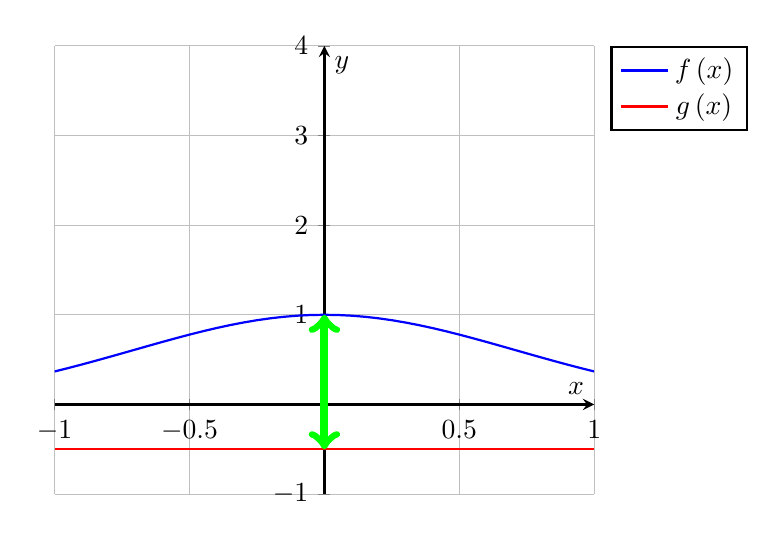
\begin{tikzpicture}[scale=1]
					\begin{axis}[
						xlabel={$x$},ylabel={$y$},
						axis lines=middle,
						samples=41,grid,thick,
						domain=-1:1,
						ymin=-1,ymax=4,
						legend pos=outer north east ]
						\addplot+[no marks] {e^-(abs(x*x))}; \addlegendentry{$f\left( x \right)$}
						\addplot+[no marks] {-0.5}; \addlegendentry{$g\left( x \right)$}
						\draw[<->,line width=1mm, color=green] (axis cs:0,-0.5) -- (axis cs:0,1);
					\end{axis}
				\end{tikzpicture}
			\end{center}
			\begin{enumerate}[label=\arabic*.]
				\item $d(x,y) \geq 0$ per definizione, il valore è sicuramente appartenente a $\realintervalclose{0}{+\infty}$, ma $+\infty$ non è un valore accettabile, in quanto la metrica è definita come funzione a valori in $\R$ e $+\infty \notin \R$. D'alto canto, si nota che $X$ è definito come l'insieme delle funzioni continue definite su un intervallo \textbf{chiuso e limitato} a valori in $\R$ ($\cntclass{0}(\realintervalclose{a}{b},\R)$). Questa definizione permette di applicare il \fullref{teo:weier_analisi_1} ed avere la certezza che esista $\sup$ finito.
				\item $d(x,y) = 0 \iff x = y$ per definizione, $d_\infty(f,g) = 0 \iff \sup\limits_{x\in\realintervalclose{a}{b}}\abs{g(x)-f(x)} = 0$, cioè se e solo se le due funzioni hanno lo stesso dominio e, per ogni punto di esso, la stessa immagine.
				\item $d(x,y)=d(y,x)$ semplicmente $d_{\infty}(f,g) = \sup\limits_{x\in\realintervalclose{a}{b}}\abs{f-g} = \sup\limits_{x\in\realintervalclose{a}{b}}\abs{g-f} = d_{\infty}(g,f)$
				\item $d(x,y) \leq d(x,z) + d(z,y)$ dalla disuguaglianza triangolare per $\abs{\;\cdot\;}$ si ottiene
					$$\abs{g(x)-f(x)}\le\abs{g(x)-h(x)}+\abs{h(x)-f(x)}$$
					Applicando il sup la disuguaglianza resta vera.
			\end{enumerate}
			\begin{note}
				Si sottolinea che queste conclusioni sono valide finché $\realintervalclose{a}{b}$ chiuso e limitato, altrimenti non varrebbe più il \fullref{teo:weier_analisi_1} necessario per il punto 1. % TODO Serve un controesempio
			\end{note}
		\item $X=\R^2$, $d$ distanza Euclidea e $P$ punto arbitrario\newline
			$\quad d_P(x,y)=
			\begin{cases}
				\begin{array}{ll}
					0 & \text{se } x = y\\
					d(x,P) + d(P,y) & \text{se } x \neq y
				\end{array}
			\end{cases}$ \hfill
			{\footnotesize
				\begin{tabular}{c}
					\textbf{Distanza di Parigi}\\
					o\\
					\textbf{Distanza Ferroviaria Francese}
				\end{tabular}
			} \label{ex:dist_parigi}
			\begin{enumerate}[label=\arabic*.]
				\item $d(x,y) \geq 0$ per definizione
				\item $d(x,y) = 0 \iff x = y$ per definizione
				\item $d(x,y)=d(y,x)$ essendo bassata sulla metrica Euclidea
				\item $d(x,y) \leq d(x,z) + d(z,y)$ essendo bassata sulla metrica Euclidea
			\end{enumerate}
		\item $X=\cntclass{0}(\realintervalclose{a}{b},\R)\;a,b\in\R,\;a<b \quad d_2(f,g) = \sqrt{\int_a^b\left[g(x)-f(x)\right]^2 \integrald{x}}$ \hfill {\footnotesize\textbf{Distanza Quadratica}}
		\label{ex:dim_dist_quadratica}
			\begin{note}
				La metrica viene trattata in \fullref{def:dist_quadratica}
			\end{note}
			\begin{enumerate}[label=\arabic*.]
				\item $d(x,y) \geq 0$ per definizione, essendo integrale di un valore positivo (quadrato) tra estremi ordinati ($a<b$ per ipotesi)
				\item $d(x,y) = 0 \iff x = y$ Per definizione della metrica, $d_2(f,g) = 0 \iff \sqrt{\int_a^b\left[g(x)-f(x)\right]^2 \integrald{x}} = 0$, cioè se e solo se le due funzioni hanno lo stesso dominio e, per ogni punto di esso, la stessa immagine.
				\item $d(x,y)=d(y,x)$ semplicmente $d_2(f,g) = \sqrt{\int_a^b\left[g(x)-f(x)\right]^2 \integrald{x}} = \sqrt{\int_a^b\left[f(x)-g(x)\right]^2 \integrald{x}} = d_2(g,f)$
				\item $d(x,y) \leq d(x,z) + d(z,y)$ ... % TODO Spiegare questo punto
			\end{enumerate}
	\end{enumerate}
\end{example}

\begin{definition}[Norma]
	\label{def:norma}
	Dato uno spazio vettoriale $V$ sul campo $\mathbb{K}$, si definisce \textbf{norma} una funzione $\norm{\cdot}:V\mapsto\R$ con le proprietà:
	\begin{enumerate}
		\item $\norm{x} \geq 0 \quad \forall x\in V$
		\item $\norm{x}=0 \iff x = 0 \quad \forall x\in V$
		\item $\norm{x+y} \leq \norm{x}+\norm{y} \quad \forall x,y\in V$
		\item $\norm{\lambda x} = \abs{\lambda} \cdot \norm{x} \quad \forall x\in V,\lambda\in\mathbb{K}$
	\end{enumerate}
	\begin{note}
		La funzione Norma associa dunque ad un vettore di qualsiasi dimensione uno scalare, fornendo (anche) una metrica per ordinare vettori tra loro.
	\end{note}
\end{definition}
\begin{definition}[Spazio Normato]
	Uno spazio normato è uno spazio vettoriale $V$ sul campo $\mathbb{K}$ \textbf{in cui è definita una norma}.
	\begin{note}
		Nel seguito verranno considerati esclusivamente spazi vettoriali su $\R$ o su $\C$, cioè $\mathbb{K} = \R$ o $\mathbb{K} = \C$
	\end{note}
\end{definition}

\begin{example}[Esempi di Spazi Normati]\leavevmode\vspace*{-\baselineskip}
	\begin{enumerate}
		\item $\R$ con $\norm{x} = \abs{x}$
		\item $\C$ con $\norm{x} = \abs{x}$
		\item $\R^n$ con $\norm{x} = \sqrt{\sum\limits_{i=1}^{n}x_i^2}$
		\item $\cntclass{0}(\realintervalclose{0}{1};\R)$ con $\norm{f} = \sup\limits_{x \in \realintervalclose{0}{1}} \abs{f(x)}$
	\end{enumerate}
\end{example}

\begin{proposition}[Metrica Indotta da una Norma]
	\label{prop:dist_sp_norm}
	Sia $V$ uno spazio normato. Allora $(V,d)$ è uno spazio metrico con la distanza
	$$d(x,y) = \norm{y-x}$$
	ed inoltre la distanza così definita è:
	\begin{enumerate}
		\item Invariante per traslazioni:
			$$\forall x,y,z \in V,\; d(x,y) = d(x+z, y+z)$$
		\item Positivamente omogenea:
			$$\forall x,y \in V\: \text{e} \forall \lambda \in \R,\; d(\lambda x, \lambda y) = \abs{\lambda}d(x,y)$$
	\end{enumerate}
	\begin{proof}
		~
		\begin{enumerate}
			\item $d(x,y) = d(x+z, y+z) = \norm{y+z-x-z} = \norm{y-x} = d(x,y)$
			\item Con la proprietà 4 della \fullref{def:norma}
			$$d(\lambda x, \lambda y) = \norm{\lambda y - \lambda x} = \norm{\lambda (y - x)} = \abs{\lambda} \norm{y - x} = \abs{\lambda}d(x,y)$$
		\end{enumerate}
	\end{proof}
	\begin{note}
		Nel caso in cui $V = \R^n$, la metrica indotta è ovviamente la \textbf{Metrica Euclidea} di \hyperref[ex:dist_eucl]{\cref*{ex:metriche} (\nameref*{ex:metriche})}
		% NOTE The \fullref command was not used on purpose to point this link straight to the right part of the aforementioned exercise
		$$d(x,y) = \sqrt{\sum\limits_{i=1}^{n} (y_i-x_i)^2 }$$
	\end{note}
\end{proposition}

\begin{definition}[Metriche Equivalenti]
	\label{def:metr_equiv}
	Siano $d_1$ e $d_2$ due distanze sullo stesso insieme $X$.
	\begin{equation*}
		\begin{gathered}
			d_1 \text{ e } d_2 \text{ sono \textbf{equivalenti}}\\
			\bydef\\
			\exists c,C \in \realintervalopen{0}{+\infty}:\; \forall x,y \in X \quad c \cdot d_1(x,y) \leq d_2 (x,y) \leq C \cdot d_1 (x,y)
		\end{gathered}
	\end{equation*}
	Cioè se è sempre possibile "limitare" una metrica con l'altra (moltiplicata per un opportuno coefficiente). Questo implica che distanze infinite per una metrica devono esserlo anche per l'altra.
	\begin{note}
		Dato uno spazio metrico $(X,d)$, passare dalla distanza $d$ ad un'altra ad essa equivalente è concettualmente analogo ad un cambio di unità di misura. Come esempio si veda \fullref{ex:dist_eqiv}
	\end{note}
\end{definition}
\begin{example}
	La \hyperref[ex:dist_parigi]{Distanza Ferroviaria Francese da \cref*{ex:metriche} (\nameref*{ex:metriche})} e la \hyperref[ex:dist_eucl]{Metrica Euclidea da \cref*{ex:metriche} (\nameref*{ex:metriche})} non sono equivalenti
	% NOTE The \fullref command was not used on purpose to point this link straight to the right part of the aforementioned exercise
	\begin{solution}
		Operando in $\R$ e avendo un $n \in \N$:
		\begin{itemize}
			\item $P = 0$
			\item $x = n$
			\item $y = n+1$
		\end{itemize}
		Ora, per ogni $n$ la $d = 1$, mentre la $d_P = 2n+1$, dunque è impossibile trovare un $C \in \realintervalopen{0}{+\infty}$ (quindi finito) tale per cui
		$$d_P(x,y) \leq C \cdot d(x,y)$$
	\end{solution}
\end{example}
\begin{example}
	\label{ex:metr_equiv_R2}
	In $\R^2$, le distanze:
	\begin{align*}
		d_1(x,y) \;\; &= \;\; \abs{y_1 - x_1} + \abs{y_2 - x_2}\\
		d(x,y) \;\; &= \;\; \sqrt{(y_1 - x_1)^2 + (y_2 - x_2)^2}\\
		d_\infty(x,y) \;\; &= \;\; \max (\abs{y_1 - x_1}, \abs{y_2 - x_2})
	\end{align*}
	sono tutte equivalenti tra di loro.
\end{example}

\definition
\begin{definition}[Sfera]
	Sia $(X,d)$ uno spazio metrico e siano $x_0 \in X$, $r > 0$. Si dice \textbf{Sfera} (o \textbf{Bolla}, o ancora \textbf{Palla}) \textbf{Aperta} di centro $x_0$ e raggio $r$ l'insieme:
	$$B(x_0,r)=\brackets{x\in X : d(x,y)<r}$$
\end{definition}
\begin{observation}
	Se $r=0\Rightarrow B(x_0,r)=\emptyset$\\
	Se $r>0\Rightarrow x_0\in B(x_0,r)$
\end{observation}
\begin{example}[Sfere ed Altri Enti]\leavevmode\vspace*{-\baselineskip}
	\begin{itemize}
		\item In $\R$ con $d$, $B(x_0,r)$ è un intervallo simmetrico centrato in $x_0$
		\item In $\R^2$ con $d$, $B(x_0,r)$ è una un cerchio con centro in $x_0$
		\item In $\R^3$ con $d$, $B(x_0,r)$ è una sfera con centro in $x_0$
	\end{itemize}
\end{example}
\begin{exercise}
	Descrivere le sfere nelle distanze dell'\fullref{ex:metr_equiv_R2}.
	% TODO soluzione
\end{exercise}

\begin{definition}[Intorno]
	Sia $(X,d)$ uno spazio metrico e sia $x \in X$. \textbf{Intorno di} $\boldsymbol{x}$ è un qualunque sottoinsieme di $X$ che contenga una sfera aperta contentente $x$
\end{definition}

\begin{definition}[Punti e Spazi Metrici]
	\label{def:pti_e_spa_metr}
	Siano $(X,d)$ uno Spazio Metrico, $A \subseteq X$ e $x_0 \in X$:
	\begin{itemize}
		\item $x_0$ \textbf{Interno} ad $A$ \quad $\bydef$ \quad $\exists r > 0:\; B(x_0, r) \subseteq A$\newline
			{\footnotesize Cioè è possibile individuare una sfera interamente contenuta in $A$}
		\item $x_0$ \textbf{Esterno} ad $A$ \quad $\bydef$ \quad $\exists r > 0:\; B(x_0, r) \subseteq X \setminus A$\newline
			{\footnotesize Cioè è possibile individuare una sfera interamente contenuta in $X$ e NON in $A$}
		\item $x_0$ \textbf{di Frontiera} per $A$ \quad $\bydef$ \quad $\forall r > 0,\; B(x_0, r) \nsubseteq A \text{ e } B(x_0, r) \nsubseteq X \setminus A$\newline
			{\footnotesize Cioè, per qualsiasi $r$, la sfera non appartiene completamente né ad $A$, né a $X \setminus A$}
		\item $x_0$ \textbf{Isolato} per $A$ \quad $\bydef$ \quad $\exists r > 0:\; B(x_0, r) \cap A = \brackets{x_0}$\newline
			{\footnotesize Cioè è possible trovare un $r$ per cui l'intersezione tra la sfera ed $A$ contiene solo $x_0$ (Esempio: i numeri naturali con $r = 0,5$)}
		\item $x_0$ \textbf{di Accumulazione} per $A$ \quad $\bydef$ \quad $\forall r > 0,\; \bigl( B(x_0, r) \cap A \bigr) \setminus \brackets{x_0} \neq \emptyset$\newline
			{\footnotesize Cioè, per qualsiasi $r$, l'intersezione tra la sfera ed $A$ è sempre non vuota (non considerando $x_0$ stesso)}
	\end{itemize}
\end{definition}
\begin{definition}
	\label{def:topologia_spa_metri}
	Siano $(X,d)$ uno spazio metrico e $A \subseteq X$. Si definisce:
	\begin{itemize}
		\item $\circdot{A} = \brackets{x \in X:\; x \text{ è interno ad } A}$ \hfill \textbf{Parte Interna di} $\boldsymbol{A}$
		\item $\partial A = \brackets{x \in X:\; x \text{ è di frontiera per } A}$ \hfill \textbf{Frontiera di} $\boldsymbol{A}$
		\item $\overline{A} = \brackets{x \in X:\; x \brackets{\text{\small\begin{tabular}{c}appartiene ad $A$\\o\\è di accumulazione per $A$\end{tabular}}}}$ \hfill \textbf{Chiusura di} $\boldsymbol{A}$
	\end{itemize}
	% TODO figura
\end{definition}
\begin{example}
	Siano $X = \R$ con $d(x,y)  = \abs{y-x}$, $A = \brackets{1} \cup \realintervalclop{2}{3}$.\\
	$1$ è un punto isolato per $A$, $5$ è esterno ad $A$.\\
	$\overline{A} = \brackets{1} \cup \realintervalclose{2}{3}$, \quad $\circdot{A} = \realintervalopen{2}{3}$, \quad $\partial A = \brackets{1, 2, 3}$
\end{example}
\begin{example}
	Sia $X = \R$ con $d(x,y)  = \abs{y-x}$\\
	Valgono le uguaglianze $\circdot{\R} = \R$, \quad $\overline{\R} = \R$, \quad $\partial \R = \emptyset$
\end{example}
\begin{proposition}
	\label{prop:chius_sp_metr}
	Siano $(X,d)$ uno spazio metrico, $A \subseteq X$, $A \neq \emptyset$. Allora
	$$\overline{A} = \brackets{x \in A \text{ è \textbf{isolato} per } A} \cup \brackets{x \in A: x \text{ è \textbf{di accumulazione} per } A}$$
	% WARNING Nel secondo elemento dell'unione, sul libro, è riportato x \in X, non x \in A. Non mi sembrava sensato, dunque l'ho cambiato in questo modo.
	\begin{proof}
		Un punto isolato, per definizione, appartiene ad $A$, e rientra quindi automaticamente nella definizione di $\overline{A}$. È dunque necessario dimostrare solo il caso $x_*$ di accumulazione per $A$.\\
		Partiamo dunque dall'ipotesi:
		\begin{align*}
			&x_* \in A \text{ e } x_* \text{ \textbf{non} isolato per } A\\
			\implies &x_* \in A \text{ e \textbf{non} } [ \exists r > 0:\; B(x_*, r) \cap A = \brackets{x_*} ]\\
			\implies &x_* \in A \text{ e } [ \forall r > 0:\; B(x_*, r) \cap A \neq \brackets{x_*} ]
			\intertext{Questo significa che in $B \cap A$ ci son sicuramente altri punti, che poi è come dire}
			\implies &x_* \in A \text{ e } \underbrace{B(x_*, r) \cap A \setminus X \neq \emptyset}_{\mathclap{\text{Definizione di punto di accumulazione}}}
		\end{align*}
	\end{proof}
\end{proposition}
\begin{proposition}
	\label{prop:relaz_sp_metr_1}
	Siano $(X,d)$ uno spazio metrico, $x_0 \in X$ e $A \subseteq X$, $A \neq \emptyset$. Allora valgono le seguenti relazioni
	\begin{enumerate}
		\item $x_0$ \textbf{isolato} per $A \implies x_0 \in A$
		\item $x_0$ \textbf{isolato} per $A \implies \begin{cases} A = \brackets{x_0}\\\qquad \text{o}\\\inf\limits_{A \setminus \brackets{x_0}} d(x,x_0) > 0\end{cases}$
		\item $x_0$ \textbf{interno} ad $A \implies x_0 \in A$
		\item $x_0$ \textbf{esterno} ad $A \iff \inf\limits_A d(x,x_0) > 0$
		\end{enumerate}
\end{proposition}
\begin{proposition}[Condizione Punti Accumulazione]
	\label{prop:condiz_punt_accumulaz}
	Siano $(X,d)$ uno spazio metrico, $x_0 \in X$ e $A \subseteq X$, $A \neq \emptyset$. Allora
	\begin{equation*}
		\begin{gathered}
			x_0 \text{ è di \textbf{accumulazione} per } A\\
			\iff\\
			\inf \brackets{d(x,x_0) : x \in A, x \neq x_0} = 0
		\end{gathered}
	\end{equation*}
	Cioè se la "minima distanza" tra $x_0$ ed un altro punto qualsiasi di $A$ è $0$.
\end{proposition}
\begin{proposition}
	\label{prop:relaz_sp_metr_2}
	Siano $(X,d)$ uno spazio metrico, $x_0 \in X$ e $A \subseteq X$, $A \neq \emptyset$. Valgono le seguenti relazioni:
	\begin{enumerate}
		\item $\overline{A} = \brackets{x_0 \in X:\; \inf\limits_{x \in A} d(x, x_0) = 0}$
		\item $\overline{\emptyset} = \emptyset$
		\item $\partial A = \overline{A} \cap \overline{X \setminus A}$
		\item $\circdot{A} \cap \partial A \neq \emptyset$
		\item $\overline{A} = \circdot{A} \cup \partial A$
	\end{enumerate}
\end{proposition}
\begin{exercise}
	Dimostrare nel dettaglio le proposizioni \fullref{prop:chius_sp_metr}, \fullref{prop:relaz_sp_metr_1}, \fullref{prop:condiz_punt_accumulaz}, \fullref{prop:relaz_sp_metr_2}.
	% TODO proofs
\end{exercise}

\begin{definition}[Insieme Aperto]
	\label{def:aperto}
	Siano $(X,d)$ uno spazio metrico e $A\subseteq X$, $A \neq \emptyset$. Si definisce
	$$A\text{ è \textbf{aperto}}\bydef A=\emptyset\quad\text{oppure}\quad A=\circdot{A}$$
\end{definition}
\begin{definition}[Insieme Chiuso]
	\label{def:chiuso}
	Siano $(X,d)$ uno spazio metrico e $A\subseteq X$, $A \neq \emptyset$. Si definisce
	$$A\text{ è \textbf{chiuso}}\bydef A=\emptyset\quad\text{oppure}\quad A=\bar{A}$$
\end{definition}
\begin{observation}
	$A$ \textbf{non chiuso} $\notimplies$ $A$ aperto\\
	$A$ \textbf{non aperto} $\notimplies$ $A$ chiuso
\end{observation}
\begin{example}
	\label{ex:ins_non_ap_non_chius}
	L'insieme $C = \brackets{(x,y) \in \R^2:\; x^2+y^2 \leq 1} \setminus \brackets{(1,0)}$ è né aperto né chiuso.
	\begin{solution}~\newline
		Non è chiuso in quanto la sua frontiera è $\partial C = \brackets{(x,y) \in \R^2:\; x^2+y^2 = 1}$, dunque $(1,0) \in \partial C$, ma per definizione $(1,0) \notin \partial C$\\
		Non è aperto in quanto, prendendo $(0,1) \in C$, è impossibile trovare un intorno di $(0,1)$ contenuto completamente in $C$
	\end{solution}
\end{example}
\begin{exercise}
	Dimostrare che in uno spazio metrico $(X,d)$:
	\begin{enumerate}
		\item Ogni sfera di raggio strettamente positivo è un aperto
		\item $\overline{B(x_0,r)} \subseteq \brackets{x \in X:\; d(x,x_0) \leq r}$
		\item $X$ è aperto ed anche chiuso
		\item $\emptyset$ è aperto ed anche chiuso
		\item Sia $A \subseteq X$. Se $A$ è aperto, allora il complementare di $A$ in $X$ è chiuso
		\item Sia $A \subseteq X$. Se $A$ è chiuso, allora il complementare di $A$ in $X$ è aperto
		\item Sia $A \subseteq X$. Allora $\overline{A}$ è chiuso e $\circdot{A}$ è aperto
	\end{enumerate}
	% TODO soluzione
\end{exercise}
\begin{proposition}
	Sia $(X,d)$ lo spazio metrico con la Metrica Discreta (da \hyperref[ex:dist_discr]{\cref*{ex:metriche} (\nameref*{ex:metriche})}).\\
	% NOTE The \fullref command was not used on purpose to point this link straight to the right part of the aforementioned exercise
	Allora, preso un $x_0 \in X$ ed un $r > 0$, l'inclusione $\overline{B(x_0,r)} \subseteq \brackets{x \in X:\; d(x,x_0) \leq r}$ è stretta se e soltanto se $r = 1$
\end{proposition}
\begin{exercise}
	Esibire in un opportuno spazio metrico esempi di insiemi né aperti né chiusi.
	% TODO examples
\end{exercise}

\begin{definition}[Diametro Spazio Metrico]
	Siano $(X,d)$ uno spazio metrico e $A\subseteq X$, $A \neq \emptyset$. Si definisce
	$$\boldsymbol{\diam}(A) \quad = \quad \sup\limits_{x,y \in A} d(x,y)$$
	Cioè la "distanza massima" tra due suoi qualsiasi elementi.
\end{definition}
\begin{definition}[Spazio Metrico Limitato]
	Siano $(X,d)$ uno spazio metrico e $A\subseteq X$, $A \neq \emptyset$. Allora
	$$A \text{ è \textbf{Limitato}} \quad \bydef \quad \diam(A) \text{ è finito}$$
	$$A \text{ è \textbf{Illimitato}} \quad \bydef \quad \diam(A) \text{ è infinito}$$
\end{definition}
\begin{note}
	L'insieme vuoto $\emptyset$ ha diametro nullo ed è dunque limitato.
\end{note}
\begin{example}[Diametri e Limitatezza in Spazi Metrici]\leavevmode\vspace*{-\baselineskip}
	\begin{enumerate}
		\item $\R$ con $d(x,y) = \abs{y-x}$ è uno spazio metrico illimitato. Inoltre se $A \subseteq \R$ con $A \neq \emptyset$, allora $\diam(A) = \sup A - \inf A$
		\item $\R$ con $d(x,y) = \frac{\abs{y-x}}{1-\abs{y-x}}$ è uno spazio metrico limitato di diametro $1$ (la distanza massima tra due punti con questa metrica è $1$)
		\item Sia $X$ un insieme con almeno $2$ elementi munito della Metrica Discreta (da \hyperref[ex:dist_discr]{\cref*{ex:metriche} (\nameref*{ex:metriche})}) è uno spazio metrico limitato di diametro $1$ % NOTE The \fullref command was not used on purpose to point this link straight to the right part of the aforementioned exercise
		\item $\cntclass{0}(\realintervalclose{0}{1}; \R)$ con $d(f,g) = \sup\limits_{\realintervalclose{0}{1}} \abs{g(x)-f(x)}$ è uno spazio metrico illimitato utilizzato in \fullref{sect:conv_unif}
	\end{enumerate}
\end{example}
\begin{exercise}
	Siano $(X,d)$ uno spazio metrico e $A,B\subseteq X$. Dimostrare le seguenti implicazioni:
	\begin{enumerate}
		\item $\left.\begin{array}{ll}
			A \subseteq B\\
			A \text{ illimitato}
			\end{array} \quad\right\} \implies B \text{ illimitato}$
		\item $\left.\begin{array}{ll}
			A \subseteq B\\
			B \text{ limitato}
			\end{array} \quad\right\} \implies A \text{ limitato}$
		\item $\left.\begin{array}{ll}
			A \text{ limitato}\\
			B \text{ limitato}
			\end{array} \quad\right\} \implies  A \cup B \text{ limitato}$
	\end{enumerate}
	% TODO soluzione
\end{exercise}
\begin{exercise}
	Dimostrare che in $\R$ le distanze
	$$d(x,y) = \abs{y-x} \quad \text{e} \quad d(x,y) = \frac{\abs{y-x}}{1+\abs{y-x}}$$
	non sono equivalenti.
	\begin{solution}
		Suggerimento: utilizzare la nozione di limitatezza.
		% TODO soluzione
	\end{solution}
\end{exercise}
\begin{exercise}
	Dimostrare che in uno spazio metrico $(X,d)$:
	\begin{enumerate}
		\item Se $x_0 \in X$ e $r > 0$, allora $\diam \bigl( B(x_0, r) \bigr) \leq 2r$ (si veda \fullref{ex:diam_sp_metr})
		\item Se $A \subseteq X$ e $x_0 \in A$, allora $A$ è limitato se e solo se esiste un $r>0:\; A \subseteq B(x_0,r)$
	\end{enumerate}
	% TODO soluzione
\end{exercise}
\begin{exercise}
	Sia $X = \R$ con la distanza $d(x,y) = \abs{y-x}$.\\
	Dimostrare che $\diam \bigl( B(0,1) \bigr) = 2$
	% TODO soluzione
\end{exercise}
\begin{exercise}
	\label{ex:diam_sp_metr}
	Sia $X = \realintervalclose{0}{2}$ con la distanza $d(x,y) = \abs{y-x}$.\\
	Dimostrare che $\diam \bigl( B(0,1) \bigr) = 1$
	% TODO soluzione
\end{exercise}

\begin{proposition}
	Siano $(X,d)$ uno spazio metrico e $A,B\subseteq X$:
	$$A \subseteq B \implies \diam(A) \leq \diam(B)$$
	\begin{proof}
		Immediata % TODO proof
	\end{proof}
\end{proposition}
\begin{exercise}
	Dimostrare con esempi che:
	\begin{enumerate}
		\item $A \subset B \notimplies \diam(A) < \diam(B)$
		\item $\diam(A) < \diam(B) \notimplies A \subset B$
		\item $\diam(A) \leq \diam(B) \notimplies A \subseteq B$
		\item $\diam(A) = 0 \notimplies A = \emptyset$ % Metrica a lunghezza zero?
	\end{enumerate}
	% TODO soluzione
\end{exercise}
\begin{exercise}
	Esibire in $\R$, $\R^2$ ed in $\cntclass{0}(\realintervalclose{0}{1}; \R)$ (con le metriche usuali) esempi di insiemi aperti/chiusi e limitati/illimtati.
\end{exercise}

\begin{definition}[Insieme Finito ed Infinito]
	Un insieme si dice \textbf{Finito} se il numero dei suoi elementi è finito.\\
	Un insieme si dice \textbf{Ininito} se non è finito.
\end{definition}
\begin{observation}
	Con la metrica Euclidea, ogni insieme finito è limitato e ogni insieme illimitato è infinito. Non valgono i viceversa.
\end{observation}

\section{Successioni e Completezza}
\begin{definition}[Successione]
	Sia $X$ un insieme non vuoto. \textbf{Successione} in $X$ è una funzione $x: \N \mapsto X$
	\begin{note}
		Altre possibili notazioni per le successioni sono: $x_n$, $(x_n)_{n \in \N}$ e $\brackets{x_n:\; n \in \N}$.\\
		Con $x_n$ si indica spesso anche \textbf{il valore assunto} dalla successione $x$ al suo $n-esimo$ elemento.
	\end{note}
\end{definition}
\begin{definition}[Successione Limitata e Illimtata]
	Una successione $x: \N \mapsto X$ di elementi di uno spazio metrico $(X,d)$ si dice \textbf{Limitata} se il suo codominio $x(\N)$ è limitato.\\
	Una successione è \textbf{Illimitata} se il suo codominio $x(\N)$ è illimitato.
\end{definition}
\begin{definition}[Limite per Successioni]
	\label{def:lim_succ}
	Data una successione $x: \N \mapsto X$ di elementi di uno spazio metrico $(X,d)$ e dato $x_\infty \in X$
	$$\lim\limits_{n \to +\infty} = x_\infty \quad \bydef \quad \lim\limits_{n \to +\infty} d(x_n,x_\infty) = 0$$
	Se $\lim\limits_{n \to +\infty} = x_\infty$, allora la successione $x_n$ è \textbf{Convergente} a $x_\infty$. Si può scrivere: $x_n \to x_\infty$ per $n \to \infty$.

	Cioè la convergenza della successione $x: \N \mapsto X$ a $x_\infty$ equivale alla convergenza a $0$ della successione di numeri reali $\brackets{d(x_n,x_\infty):\; n \in \N}$
	\begin{note}
		Essendo posto $x_\infty \in X$, $x_\infty$ deve appartenere allo spazio metrico. In caso alternativo il limite non esiste.
	\end{note}
	\begin{note}
		Questa definizione è \textit{implicita}, cioè non porta a nessun metodo \textit{costruttivo} per calcolare il limite di una successione. La definizione di limite permette soltanto di verificare se una nota quantità è limite della successione data o meno.
	\end{note}
\end{definition}
\begin{proposition}
	\label{prop:succ_conv_lim}
	Data la successione $x: \N \mapsto X$ di elementi dello spazio metrico $(X,d)$ e dato $x_\infty\in X$:
	$$\lim\limits_{n\rightarrow+\infty}x_n = x_\infty \quad \iff \quad \forall\varepsilon > 0 \quad \exists\nu\in\N:\; \forall n>\nu \text{ vale } d(x_n,x_\infty)<\varepsilon$$
	\begin{proof}
		% TODO dimostrazione
	\end{proof}
\end{proposition}
\begin{theorem}[Teorema di Unicità del Limite per Successioni]
	Sia $(X,d)$ uno spazio metrico e siano $x_\infty, x^\infty$ elementi di $X$ e $x: \N \mapsto X$ una successione in $X$.
	\begin{equation*}
		\left.
		\begin{array}{l}
			\lim\limits_{n \to +\infty} x_n = x_\infty\\
			\lim\limits_{n \to +\infty} x_n = x^\infty\\
		\end{array}
		\quad\right\}
		\implies x_\infty = x^\infty
	\end{equation*}
	\begin{proof}
		Per ogni $n \in \N$, per la proprietà 4 da \fullref{def:sp_metrico}
		$$d(x_\infty, x^\infty) \leq d(x_\infty, x_n) + d(n, x^\infty)$$
		Passando al $\lim$ per $n \to +\infty$
		$$\underbrace{\lim\limits_{n \to +\infty}d(x_\infty, x^\infty)}_{\begin{tabular}{c}\geq 0\\{\small Per def. distanza}\end{tabular}}
		\leq
		\underbrace{\lim\limits_{n \to +\infty}d(x_\infty, x_n)}_{\begin{tabular}{c}\leq \varepsilon\\{\small Per def. lim succ.}\end{tabular}}
		+
		\underbrace{\lim\limits_{n \to +\infty}d(n, x^\infty)}_{\begin{tabular}{c}\leq \varepsilon\\{\small Per def. lim succ.}\end{tabular}}
		\leq 2 \varepsilon$$
		Dovendo essere questa forma valida $\forall \varepsilon > 0$, si concludere che non può esser altro che
		$$\lim\limits_{n \to +\infty}d(x_\infty, x^\infty) = 0$$
		Che, per la proprietà 2 da \fullref{def:sp_metrico}, significa
		$$x_\infty = x^\infty$$
	\end{proof}
\end{theorem}
\begin{proposition}
	\label{prop:succ_conv_se_comp_conv}
	Sia $p \in \N,\; p \geq 2$. In $\R^p$, con $d(x,y) = \norm{y-x}$, una successione $x: \N \to X$ converge a $x_\infty$ se e solo se le $è$ successioni delle componenti convergono alle rispettive componenti di $x_\infty$.
	\begin{proof}
		Applicare la \fullref{def:lim_succ} ricordando che
		$$\abs{y_i} \leq \norm{y} \leq \abs{\sum\limits_{i = 1}^p \abs{y_i}} \qquad \forall y \in \R^p \text{ e per } i = 1,\:\dotsc\:,p$$
		% TODO actual proof
	\end{proof}
\end{proposition}
\begin{exercise}
	Esibire un esempio di successione in $\R^2$ convergente a $(1,1)$ con le distanze introdotte ai punti 3 e 4 dell'\fullref{ex:metriche}.
	% TODO soluzione
\end{exercise}
\begin{exercise}
	Esibire un esempio di successione in $\C$ convergente a $1+i$ con la distanza $d(z,w) = \abs{w-z}$.
	% TODO soluzione
\end{exercise}
\begin{proposition}[Caratterizzazione dei Punti di Accumulazione]
	\label{prop:caratteriz_pti_accumul}
	Siano $(X,d)$ uno spazio metrico, $A \subseteq X$ e $x_* \in X$. Allora
	$$x_* \text{ di accumulazione per } A \iff
	\begin{cases}
		\begin{tabular}{c} % NOTE This should probably be a box of some kind instead of a tabular
			esiste una successione di elementi di $A$,\\
			diversi da $x_*$, convergente a $x_*$
		\end{tabular}
	\end{cases}$$
	\begin{proof}~
		\begin{itemize}
			\item[$\implies$] Grazie alla \fullref{prop:condiz_punt_accumulaz}
				\begin{align*}
					&x_* \text{ è di accumulazione per } A\\
					\implies &\inf \brackets{d(x,x_*):\; x \in A, x \neq x_0} = 0
					\intertext{Che equivale a scrivere}
					\implies &\forall \varepsilon > 0\: \exists x_\varepsilon \in A:\; x_\varepsilon \neq x_* \text{ e } d(x_\varepsilon, x_*) < \varepsilon
					\intertext{Quindi si può scegliere arbitrariamente un $\varepsilon = \frac{1}{n}$, ponendo $n \neq 0$ ed arrivare a}
					\implies &\forall n \in \N \setminus \brackets{0},\: \exists x_n \in A:\; x_n \neq x_* \text{ e } d(x_n,x_*) < \frac{1}{n}
				\end{align*}
				La successione delle distanze è convergente a $0$ per $n \to +\infty$, quindi con la \fullref{def:lim_succ} si può concludere che la successione $x_n$ converge a $x_*$
			\item[$\impliedby$] Dalla \fullref{def:lim_succ}
				$$\forall\varepsilon > 0 \quad \exists\nu\in\N:\; \forall n>\nu \quad x_n \in A,\: x_n \neq x_*, \quad d(x_n,x_*)<\varepsilon$$
				Ma se $d(x_n,x_*)<\varepsilon$, allora si può anche scrivere $x_n \in B(x_*, \varepsilon)$, quindi sicuramente
				\begin{align*}
					\implies & \forall\varepsilon > 0 \quad B(x_*, \varepsilon) \cap A \setminus \brackets{x_*} \neq \emptyset\\
					\intertext{Dunque stando alla \fullref{def:pti_e_spa_metr}}
					\implies & x_* \text{ è di accumulazione per } A
				\end{align*}
		\end{itemize}
	\end{proof}
\end{proposition}
\begin{corollary}
	\label{coro:succ_conv_sse_x_in_chius_A}
	Siano $(X,d)$ uno Spazio Metrico, $A \subseteq X$ e $x_* \in X$. Allora:
	$$x_* \in \overline{A} \iff
	\begin{cases}
		\begin{tabular}{c} % NOTE This should probably be a box of some kind instead of a tabular
			esiste una successione di elementi di $A$,\\
			diversi da $x_*$, convergente a $x_*$
		\end{tabular}
	\end{cases}$$
	\begin{proof}~
		\begin{itemize}
			\item[$\implies$]
				\begin{itemize}
					\item Se $x_* \in A$\newline
						È sufficiente scegliere $x_n = x_*$, successione costante, dunque
						$$\lim\limits_{n \to +\infty} x_n = \lim\limits_{n \to +\infty} x_* = x_*$$
					\item Se $x_*$ di accumulazione per $A$\newline
						Per \fullref{def:topologia_spa_metri} e grazie alla \fullref{prop:caratteriz_pti_accumul} si giunge direttamente alla tesi.
				\end{itemize}
			\item[$\impliedby$] Per \fullref{def:topologia_spa_metri} e grazie alla \fullref{prop:caratteriz_pti_accumul} si giunge direttamente alla tesi.
		\end{itemize}
	\end{proof}
\end{corollary}

\begin{definition}[Condizione di Cauchy]
	Sia $(X,d)$ uno spazio metrico e $x: \N \mapsto X$ una successione d in $X$.
	\begin{equation}
		\begin{gathered}
			x:\N \mapsto X \text{ è \textbf{di Cauchy}}\\
			\bydef\\
			\forall \varepsilon > 0\quad \exists \nu \in \N:\; \forall n,m > \nu \text{ vale } d(x_n, x_m) < \varepsilon
		\end{gathered}
	\end{equation}
	Cioè se la distanza tra due punti qualsiasi della successione, presi dopo un certo valore $\nu$, è minore di un $\varepsilon$ piccolo a piacere.
	\begin{note}
		Questa definizione, differentemente dalla \fullref{def:lim_succ}, è \textit{esplicita} e \textit{intrinseca}: dipende esclusivamente dalla successione e dalla distanza definita.
	\end{note}
\end{definition}
\begin{proposition}
	\label{prop:se_succ_conv_allora_cau}
	Sia $(X,d)$ uno spazio metrico.
	$$x: \N \mapsto X \text{ è \textbf{convergente} } \implies x:\N \mapsto X \text{ è \textbf{di Cauchy}}$$
	\begin{proof}
		Sia $x: \N \mapsto X$ convergente a $x_\infty$. Allora
		$$\lim\limits_{n \to +\infty} x_n \bydef \forall\varepsilon > 0 \quad \exists\nu\in\N:\; \forall n > \nu \quad d(x_n,x_\infty)<\varepsilon$$
		Prendendo dunque due elementi qualsiasi $n$ e $m$ con $n,m > \nu$, la distanza di ognuno di essi da $x_\infty$ dovrà essere $<\varepsilon$. Applicando la proprietà 4 da \fullref{def:sp_metrico}, otteniamo
		$$d(x_n,x_m) \leq \left[ d(x_n,x_\infty)+d(x_m,x_\infty) \right] < 2\varepsilon$$
		Quindi
		$$\forall\varepsilon > 0 \quad \exists\nu\in\N:\; \forall n,m > \nu \quad d(x_n,x_m) \leq \left[ d(x_n,x_\infty)+d(x_m,x_\infty) \right] < 2\varepsilon$$
		Cioè ci si è ricondotti alla definizione della Condizione di Cauchy
	\end{proof}
\end{proposition}

\begin{definition}[Spazio Metrico Completo]
	\label{def:completo}
	Uno Spazio Metrico $(X,d)$ si dice \textbf{Completo} se e solo se \textbf{ogni successione di Cauchy in $X$ ammette limite in $X$ stesso}.
\end{definition}
\begin{example}[Esempi di Spazi Metrici Completi e non]\leavevmode\vspace*{-\baselineskip}
	\begin{enumerate}
		\item $\R$ con $d(x,y) = \abs{y - x}$ è uno spazio metrico completo
		\item $\mathbb{Q}$ con $d(x,y) = \abs{y - x}$ è uno spazio metrico \textit{non} completo
		\item $\R^n$ con $d(x,y) = \norm{y - x}$ è uno spazio metrico completo.\\
			Altre distanze che rendono $\R^n$ uno spazio metrico completo sono, ad esempio
			\begin{itemize}
				\item $d(x,y) = \max\limits_{i=1,\:\dotsc\:,n} \abs{y_i - x_i}$
				\item $d(x,y) = \left( \sum\limits_{i=1}^{n} \abs{y_i - x_i}^\alpha \right)^{\frac{1}{\alpha}}$ con $\alpha \in \realintervalclop{1}{+\infty}$
			\end{itemize}
		\item $\realintervalopen{0}{1}$ con $d(x,y) = \abs{y - x}$ è uno spazio metrico \textit{non} completo.
			\begin{proof}
				La successione $\brackets{\frac{1}{n}:\; n \in \N, n \neq 0}$ è di Cauchy ma non ammette limite in $\realintervalopen{0}{1}$
			\end{proof}
		\item Sia $X$ un insieme con almeno 2 elementi, munito della metrica discreta
			$$d(x,y)=
			\begin{cases}
				\begin{matrix}
					0&&x=y\\
					1&&x \ne y
				\end{matrix}
			\end{cases}$$
			$X$ è uno spazio metrico completo in cui le uniche successioni convergenti son le successioni \textbf{definitivamente costanti} (cioè costanti da un certo indice in poi).
		\item $\cntclass{0}(\realintervalclose{0}{1}; \R)$ è uno spazio metrico completo con la distanza
			$$d(f,g) = \sup\limits_{\realintervalclose{0}{1}}\abs{g(x) - f(x)}$$
			Vedasi \fullref{prop:dist_unif_sp_metr_compl} per la dimostrazione.
		\item $\cntclass{0}(\realintervalclose{0}{1}; \R)$ è uno spazio metrico \textit{non} completo con la distanza
			$$d(f,g) = \sqrt{\int_0^1 \left[ g(x) - f(x) \right]^2 \integrald{x}}$$
			Vedasi \fullref{prop:dist_quad_sp_metr_non_compl} per la dimostrazione.
		\item L'insieme $\C$ dei numeri complessi è uno spazio metrico completo con la distanza $d(z,w) = \abs{w-z}$
	\end{enumerate}
\end{example}
\begin{exercise}
	Esibire una successione di Cauchy di numeri razionali non convergente in $\mathbb{Q}$.
	\begin{solution}
		La seguente successione
		$$\lim\limits_{n \to +\infty} \left( 1+ \frac{1}{n} \right)^n$$
		è convergente a $e \notin \mathbb{Q}$
	\end{solution}
\end{exercise}
\begin{proposition}
	\label{prop:subset_compl_e_compl}
	Siano $(X,d)$ uno spazio metrico \textbf{completo} e $C \subseteq X$ un sottoinsieme \textbf{chiuso} di $X$. Allora $\boldsymbol{(C,d_{|C})}$ \textbf{è sottospazio metrico completo}, con $d_{|C}$ da \fullref{def:metr_indotta}.
	\begin{proof}
		Essendo $C$ chiuso, per \fullref{def:chiuso}:
		$$C = \overline{C} \implies \forall x_* \in C\; x_* \in \overline{C}$$
		Si può dunque applicare il \fullref{coro:succ_conv_sse_x_in_chius_A} e concludere che
		$$\forall x_* \in C \text{ esiste un successione di elementi di $C$ convergenti a $x_*$}$$
		Questo permette di individuare tante successioni $x_i$ quanti sono gli elementi di $C$ e, grazie alla \fullref{prop:se_succ_conv_allora_cau}, si sa che ognuna di queste successioni è di Cauchy.

		Si giunge dunque alla \fullref{def:completo}
	\end{proof}
	\begin{note}
		La chiusura di $C$ è fondamentale perché diversamente non sarebbe applicabile il \fullref{coro:succ_conv_sse_x_in_chius_A} e dunque non si avrebbe certezza sulla convergenza in $C$ delle successioni.
	\end{note}
\end{proposition}
\begin{proposition}
	\label{prop:se_cau_allora_lim}
	Sia $(X,d)$ uno spazio metrico. Data la successione $x: N \mapsto X$ \textbf{di Cauchy}:
	$$x: N \mapsto X \text{\textbf{ di Cauchy}} \implies x: N \mapsto X \text{\textbf{ limitata}}$$
	\begin{proof}
		\begin{equation*}
			\begin{gathered}
				x: N \mapsto X \text{ di Cauchy}\\
				\bydef\\
				\forall \varepsilon > 0\quad \exists \nu \in \N:\; \forall n,m > \nu \text{ vale } d(x_n, x_m) < \varepsilon
			\end{gathered}
		\end{equation*}
		La dimostrazione prevede di dividere in due "parti" la successione
		\begin{enumerate}
			\item Per la definizione di cui sopra è sicuramente possibile individuare un certo $\overline{\nu}$ per cui
				$$\exists \overline{\nu}:\; \forall n > \overline{\nu} \quad d(x_n, x_{\overline{\nu}}) < 1 \text{ (1 è scelto arbitrariamente)}$$
				In tal modo è stata esplicitata la limitatezza di $x$ \textit{da $\overline{\nu}$ in poi}.
			\item Si ponga invece $K = \max\limits_{n=0,\: \dotsc \:, \overline{\nu}-1} d(x_n, x_{\overline{\nu}})$, cioè $K$ è la massima tra tutte le distanze $d(x_n, x_{\overline{\nu}})$ con $n < \overline{\nu}$.\\
				Essendo $n < \overline{\nu}$, $n$ è sicuramente finito, per cui anche $K$ sarà finito. Infatti, avendo un numero finito $n$ di valori $x_n$ assunti dalla successione, anche il massimo di tali valori (cioè $K$) sarà finito.\\
				In questo modo si è trovato un valore $K$ che limita la $x$ \textit{prima di} $\overline{\nu}$.
		\end{enumerate}
		Quindi, concludendo, sicuramente
		$$\forall n \in \N \quad d(x_n, x_{\overline{\nu}}) < \max \brackets{K, 1}$$
		Cioè la successione è limitata.
	\end{proof}
\end{proposition}
\begin{exercise}
	\label{ex:succ_lim_non_cau}
	Definire in un opportuno spazio metrico una successione limitata non di Cauchy.
	\begin{solution}
		In $(\N,d)$ la successione $x(n) = (-1)^n$.
	\end{solution}
\end{exercise}
\begin{corollary}
	Sia $(X,d)$ uno spazio metrico. Data la successione $x: N \mapsto X$ \textbf{convergente}:
	$$x: N \mapsto X \text{\textbf{ convergente}} \implies x: N \mapsto X \text{\textbf{ limitata}}$$
	\begin{proof}
		Grazie alla \fullref{prop:se_succ_conv_allora_cau} ed alla \fullref{prop:se_cau_allora_lim}
		$$\text{convergente } \implies \text{ di Cauchy } \implies \text{ limitata}$$
	\end{proof}
\end{corollary}
\begin{exercise}
	Definire in un opportuno spazio metrico una successione limitata non convergente.
	\begin{solution}
		Come da \fullref{ex:succ_lim_non_cau} % TODO magari un'altra successione qui
	\end{solution}
\end{exercise}
\begin{exercise}
	Siano $(X,d)$ uno spazio metrico completo, $A \subseteq X$ chiuso e non vuoto. Allora, detta $d_{|A}$ la restrizione di $d$ ad $A$, $(A,d_{|A})$ è uno spazio metrico completo.\\
	È indispensabile l'ipotesi "\textit{$A$ chiuso}"?
	\begin{solution}
		Vedere nota alla \fullref{prop:subset_compl_e_compl}
	\end{solution}
\end{exercise}
\begin{exercise}
	Dimostrare che ogni sottosuccessione di una successione di Cauchy è a sua volta una successione di Cauchy.
	% TODO soluzione
\end{exercise}
\begin{exercise}
	\label{ex:sottsucc_conv_succ_conv}
	Dimostrare che se una successione ammette una sottosuccessione convergente, allora l'intera successione è convergente.
	% TODO soluzione
\end{exercise}

\subsection{Insiemi Connessi}
Concettualmente, un insieme è connesso se è \textit{un pezzo solo}. Per dare una definizione formale conviene prima caratterizzare gli insiemi formati \textit{da più pezzi} e poi definire come connessi quelli \textit{non} formati \textit{da più pezzi}.
\begin{definition}[Insiemi Separati]
	Siano $(X,d)$ uno spazio metrico, $A \subseteq X$ e $B \subseteq X$
	$$A \text{ e } B \text{ sono \textbf{Separati}} \bydef \overline{A} \cap B = \emptyset \text{ e } A \cap \overline{B} = \emptyset$$
\end{definition}
\begin{definition}[Insieme Connesso o Sconnesso]
	Un insieme è \textbf{Sconnesso} se e solo se è \textbf{unione} di due insiemi \textbf{separati}.\\
	Un insieme è \textbf{Connesso} se e solo se \textbf{non è Sconnesso}.
	\begin{note}
		In uno spazio metrico un insieme può essere alternativamente connesso o sconnesso, ma sicuramente deve essere di un tipo o dell'altro. Ciò differisce con la classificazione Aperto/Chiuso secondo la quale potevano esistere insiemi né aperti né chiusi (vedasi \fullref{ex:ins_non_ap_non_chius})
	\end{note}
\end{definition}
\begin{example}
	In $\R$ con l'usuale distanza Euclidea:
	\begin{enumerate}
		\item $\realintervalclose{0}{1}$ e $\realintervalopcl{1}{2}$ non sono separati
		\item $\realintervalclop{0}{1}$ e $\realintervalopcl{1}{2}$ sono separati
		\item $\brackets{0} \cup \realintervalclose{1}{2}$ è sconnesso
		\item $\R$ è connesso
	\end{enumerate}
\end{example}
\begin{exercise}
	Dimostrare che gli insiemi $\N$, $\mathbb{Z}$ e $\mathbb{Q}$ sono sottoinsiemi sconnessi di $\R$ con la distanza Euclidea.
	% TODO soluzione
\end{exercise}
\begin{exercise}
	Dimostrare che se due insiemi sono separati, allora sono disgiunti. Esibire un controesempio all'implicazione inversa.
	% TODO soluzione
\end{exercise}
\begin{exercise}
	Esibire esempi di insiemi:
	\begin{enumerate}
		\item connessi/sconnessi ed aperti/chiusi
		\item connessi/sconnessi e limitati/illimitati
	\end{enumerate}
	% TODO soluzione
\end{exercise}

\begin{proposition}
	In $\R$ con la metrica Euclidea, sia $A \subseteq \R$.
	$$A \text{ è \textbf{Connesso}} \iff A \text{ è un \textbf{Intervallo}}$$
	\begin{proof}
		Omessa.
	\end{proof}
\end{proposition}
\begin{proposition}[Poligonale Congiungente due Punti]
	\label{prop:polig_in_aperto_connesso}
	In $\R^n$ con la distanza Euclidea, sia $A$ un \textbf{aperto connesso}. Allora, comunque scelti $x$ e $y$ in $A$, esiste una \textbf{poligonale} interamente contenuta in $A$ con i lati paralleli agli assi e congiungente $x$ a $y$.
	% TODO disegno
	\begin{proof}
		Omessa.
	\end{proof}
\end{proposition}
\begin{exercise}
	Mostrare con un esempio che nella \fullref{prop:polig_in_aperto_connesso} l'ipotesi "\textit{$A$ aperto}" è essenziale.
	\begin{solution}
		Dato lo spazio metrico $(\R^2,d)$, tutti i punti del sottoinsieme $\brackets{x \in \R^2:\;x^2 + y^2 = 1}$ sono di frontiera, dunque non è un aperto. È impossibile individuare una poligonale che colleghi due qualsiasi punti della circonferenza in quanto, appunto circonferenza.
	\end{solution}
\end{exercise}

\subsection{Insiemi Compatti}
\begin{definition}[Insieme Compatto]
	\label{def:compatto}
	Siano $(X,d)$ uno spazio metrico e $A \subseteq X$. $A$ è \textbf{Compatto} se e solo se \textbf{ogni successione di elementi di $A$ ammette una sottosuccessione avente limite in $A$}.
	\begin{note}
		Questa è la definizione di \textbf{Compattezza per Successioni}, in spazi più generali può essere necessario utilizzare una definizione più debole che, nel caso degli spazi metrici, coincide con la precedente.
	\end{note}
\end{definition}
\begin{proposition}
	\label{prop:compat_chius_lim}
	Siano $(X,d)$ uno spazio metrico e $A \subseteq X$
	$$A \text{ \textbf{compatto}} \implies A \text{ \textbf{chiuso e limitato}}$$
	\begin{proof}
		Per assurdo negando una per una le conclusioni.
		\begin{itemize}
			\item $A$ non è chiuso
				\begin{align*}
					&A \text{ non è chiuso}\\
					\implies &A \neq \overline{A}\\
					\implies &A \subset \overline{A}\\
					\implies &\exists x_0 \in \overline{A},\; x_0 \notin A\\
					\shortintertext{Dunque, per \fullref{def:topologia_spa_metri}, si deve concludere che}
					\implies &\exists x_0 \text{ di accumulazione per } A,\; x_0 \notin A\\
					\shortintertext{Quindi dalla \fullref{prop:caratteriz_pti_accumul}}
					\implies &x:\; \N \mapsto X \text{ con }
						\begin{cases}
							x_n \in A\; \forall n\\
							\lim\limits_{n \to +\infty} x_n = x_0, x_0 \notin A
						\end{cases}\\
					\shortintertext{Cioè abbiamo ottenuto una successione non convergente in $A$, dunque negando l'ipotesi}
					\implies &A \text{ non è compatto - \textit{Assurdo}}
				\end{align*}
			\item $A$ non è limitato
				\begin{align*}
					&A \text{ non è limitato}\\
					\implies &\sup \brackets{d(x,y): x,y \in A} = + \infty\\
					\shortintertext{Fissato dunque un $x_0 \in A$, continuerò ad aver distanza infinita, in quanto $A$ non limitato per ipotesi.}
					\implies &\sup\limits_{x \in A} d(x,x_0) = + \infty\\
					\implies &\forall n \in \N,\; \exists x_n \in A:\; d(x_n, x_0) > n
					\shortintertext{Dunque qualsiasi sottosuccessione di $x:\; \N \mapsto X$ è illimitata}
					\implies &x:\; \N \mapsto X \text{ è una successione in $A$ senza sottosuccessioni convergenti}\\
					\implies &A \text{ non è compatto - \textit{Assurdo}}
				\end{align*}
		\end{itemize}
	\end{proof}
\end{proposition}
\begin{proposition}
	\label{prop:compat_chius_lim_Rn}
	In $\R^n$ con l'usuale metrica Euclidea, sia $A \subseteq \R^n$. Allora:
	$$A \text{ è \textbf{Compatto}} \iff A \text{ è \textbf{Chiuso e Limitato}}$$
	\begin{proof}
		Omessa a lezione.\\
		\color{not_explained_section_color}
		Nel caso $n = 1$, segue dalle (note) proprietà di $\R$. Nel caso $n > 1$, si veda \fullref{ex:compat_chius_lim_Rn}.
		\color{black}
	\end{proof}
\end{proposition}
\begin{note}
	La \fullref{prop:compat_chius_lim} vale in ogni spazio metrico, mentre la \fullref{prop:compat_chius_lim_Rn} solo in $A \subseteq R^n$
\end{note}
\color{not_explained_section_color}
\begin{exercise}
	\label{ex:compat_chius_lim_Rn}
	Completare la dimostrazione della \fullref{prop:compat_chius_lim_Rn}.\\
	Suggerimento: utilizzare il caso $n = 1$ e la e la \fullref{prop:succ_conv_se_comp_conv}
\end{exercise}
\begin{exercise}
	Confrontare la dimostrazione della \fullref{prop:compat_chius_lim_Rn} con \fullref{ex:BBBBBBBBBB}
\end{exercise}
\color{black}
\begin{exercise}
	In uno spazio metrico, esibire esempi di insiemi connessi/sconnessi e compatti/non compatti.
	% TODO solution
\end{exercise}
\begin{exercise}
	In $\R$ con la distanza Euclidea, esibire esempi di insiemi che siano itnervalli/non intervalli compatti/non compatti
	% TODO solution
\end{exercise}
\begin{exercise}
	\label{ex:unione_compatti}
	Sia $(X,d)$ uno spazio metrico. Siano $K_1$ e $K_2$ due sottoinsiemi compatti di $X$. Allora $K_1 \cup K_2$ è compatto
	\begin{solution}
		Posto $K = K_1 \cup K_2$, per definizione di \textbf{unione}, ogni elemento di $K$ è in $K_1$ o $K_2$.\\
		Visto che, per ipotesi, $K_1$ e $K_2$ sono compatti, sappiamo che ogni successione in uno dei due avrà una sottosuccessione convergente nello stesso insieme. A questo punto possiamo concludere che ogni successione in $K$ ammetterà una sottosuccessione convergente ad un elemento $x_\infty \in K_1$ oppure $x_\infty \in K_2 \implies x_\infty \in K$
	\end{solution}
\end{exercise}

\begin{proposition}
	Sia $(X,d)$ uno spazio metrico. Allora
	$$X \text{ è \textbf{Compatto}} \implies X \text{ è \textbf{Completo}}$$
	\begin{proof}
		Sia $x: \N \mapsto X$ una successione di Cauchy di elementi di $X$.\\
		$X$ è compatto quindi, per definizione, esiste una sottosuccessione convergente ad un $x_\infty \in X$. Ciò implica, grazie all'\fullref{ex:sottsucc_conv_succ_conv}, che l'intera successione converga a $x_\infty$, dunque $X$ è completo.
	\end{proof}
\end{proposition}

\begin{observation}
	Sia $X$ un insieme munito di due distanze tra loro equivalenti $d_1$ e $d_2$ (si veda \fullref{def:metr_equiv}). Allora \textit{ciò che vale in $(X, d_1)$, vale in $(X, d_2)$}\\
	Il seguente esercizio rende rigorosa questa affermazione
\end{observation}
\begin{exercise}
	\label{ex:dist_eqiv}
	Sia $X$ un insieme munito delle due distanze $d_1$ e $d_2$ tra loro equivalenti. \textbf{Se un insieme è aperto} (chiuso, compatto, connesso, limitato) \textbf{in} $\boldsymbol{(X,d_1)}$, allora \textbf{lo è anche in} $\boldsymbol{(X,d_2)}$.\\
	Inoltre, \textbf{se} $\boldsymbol{\lim\limits_{n \to +\infty} x_n = x_\infty}$ \textbf{in} $\boldsymbol{(X,d_1)}$, allora $\boldsymbol{\lim\limits_{n \to +\infty} x_n = x_\infty}$ \textbf{anche in in} $\boldsymbol{(X,d_2)}$
	% TODO solution
\end{exercise}
\begin{example}
	Sia $(X,d)$ lo spazio $\R^n$ munito della distanza Euclidea. Sia $d_p$ come in \hyperref[ex:dist_parigi]{\cref*{ex:metriche} (\nameref*{ex:metriche})} con $p \in \R^n$\\
	% NOTE The \fullref command was not used on purpose to point this link straight to the right part of the aforementioned exercise	
	È interessante notare che in $(X,d)$, $d_p$ stessa non è continua e quindi gli insiemi aperti (chiusi) rispetto a $d_p$, possono non essere aperti (chiusi) rispetto alla distanza Euclidea. Di conseguenza son proprietà diverse nei due spazi metrici: convergenza di successioni, continuità di funzioni, connessione, compattezza, essere o meno punto di accumulazione, punto interno, punto esterno\dots
\end{example}
\begin{exercise}
	Siano $(X,d)$ uno spazio metrico e $A \subseteq X$ un \textbf{compatto}. Dimostrare che se $C \subseteq A$ \textbf{è un chiuso}, allora è anche \textbf{compatto}.\\
	L'ipotesi "\textit{$C$ chiuso}" è indispensabile? 
\end{exercise}

\section{Limiti e Continuità}
\begin{definition}[Limite per Funzione]
	\label{def:lim_funz}
	Siano:
	\begin{itemize}
		\item $(X,d_X)$ e $(Y,d_Y)$ spazi metrici
		\item $A \subseteq X$
		\item $x_0$ di accumulazione per $A$
		\item $f:\; A \mapsto Y$ una funzione
		\item $l \in Y$
	\end{itemize}
	Allora si definisce
	\begin{equation*}
		\begin{gathered}
			\lim\limits_{x \to x_0} f(x) = l\\
			\bydef\\
			\forall \varepsilon > 0,\; \exists \delta > 0:\; \forall x \in A \text{ con } d_X(x,x_0) < \delta \text{ e } x \neq x_0 \text{ vale } d_Y(f(x),l)<\varepsilon
		\end{gathered}
	\end{equation*}
	Che si legge \textit{il limite per $x$ tendente a $x_0$ di $f(x)$ converge a $l$ per $x$ tendente a $x_0$}.
\end{definition}
\begin{exercise}
	Sarebbe comodo definire
	\begin{equation*}
		\begin{gathered}
			\lim\limits_{x \to x_0} f(x) = l\\
			\bydef\\
			\lim\limits_{x \to x_0} d(f(x), l) = 0
		\end{gathered}
	\end{equation*}
	Perché non è corretto farlo?
	\begin{solution}
		Non è corretto perché questa definizione implica $l = f(x)$ con $x \to x_0$ per proprietà 2 di \fullref{def:sp_metrico}. Ciò è diverso aalla \fullref{def:lim_funz} ed è inoltre più restrittivo, in quanto, con questa definizione "semplificata", sarebbe richiesto $x_0 \in A$, mentre $x_0$ deve essere solo di accumulazione nell'altro caso. Un punto di accumulazione non è necessariamente incluso nell'insieme a cui è riferito.
	\end{solution}
\end{exercise}

\begin{theorem}[Teorema di Unicità del Limite per Funzioni]
	Siano $(X,d_X)$ e $(Y,d_Y)$ spazi metrici, $A \subseteq X$, $x_0$ di accumulazione per $A$, $f:\; A \mapsto Y$ una funzione e $l', l'' \in Y$
	\begin{equation*}
		\left.
		\begin{array}{c}
			\lim\limits_{x \to x_0} f(x) = l'\\
			\lim\limits_{x \to x_0} f(x) = l''
		\end{array}
		\right\}
		\implies l' = l''
	\end{equation*}
	\begin{proof}
		\begin{equation*}
			\begin{gathered}
				\left.
				\begin{array}{c}
					\lim\limits_{x \to x_0} f(x) = l'\\
					\lim\limits_{x \to x_0} f(x) = l''
				\end{array}
				\right\} \implies\\
				\implies
				\begin{cases}
					\forall \varepsilon > 0,\; \exists \delta' > 0:\; \forall x \in A \text{ con } d_X(x,x_0) < \delta' \text{ e } x \neq x_0 \text{ vale } d_Y(f(x),l')<\varepsilon\\
					\forall \varepsilon > 0,\; \exists \delta'' > 0:\; \forall x \in A \text{ con } d_X(x,x_0) < \delta'' \text{ e } x \neq x_0 \text{ vale } d_Y(f(x),l'')<\varepsilon
				\end{cases}
			\end{gathered}
		\end{equation*}
		Posto $\delta = \min \brackets{\delta', \delta''}$, si può sicuramente concludere
		\begin{equation*}
			\begin{gathered}
				\forall \varepsilon > 0,\; \exists \delta > 0:\; \forall x \in A \text{ con } d_X(x,x_0) < \delta \text{ e } x \neq x_0 \text{ vale } d_Y(f(x),l')<\varepsilon \text{ e vale } d_Y(f(x),l'') <\varepsilon\\
				\implies \forall \varepsilon > 0 \quad d_Y(l', l'') < 2 \varepsilon\\
				\implies d_Y(l', l'') = 0
			\end{gathered}
		\end{equation*}
	\end{proof}
\end{theorem}

\begin{proposition}[Continuità per Successioni]
	\label{prop:funz_cont_per_succ}
	Siano $(X,d_X)$ e $(Y,d_Y)$ spazi metrici, $A \subseteq X$, $x_0$ di accumulazione per $A$, $f:\; A \mapsto Y$ e $l \in Y$
	\begin{equation*}
		\begin{gathered}
			\lim\limits_{x \to x_0} f(x) = l\\
			\iff\\
			\forall \text{ successione } x: \N \mapsto X \text{ tale che } \lim\limits_{x \to +\infty} x_n = x_0 \text{ e } x_n \neq x_0\\
			\text{vale} \lim\limits_{n \to +\infty} f(x_n) = l
		\end{gathered}
	\end{equation*}
	\begin{note}
		Specificare "\textit{$\forall$ successione}" è fondamentale in quanto bisogna considerare tutti i punti $x \in A$, non solo le divisioni discrete degli $n \in \N$
	\end{note}
	\begin{proof}~
		\begin{itemize}
			\item[$\implies$] Dalle \fullref{def:lim_funz} e \fullref{def:lim_succ}
				\begin{align*}
					\lim\limits_{x \to x_0} f(x) = l &\implies
					\begin{cases}
						\forall \varepsilon > 0,\; \exists \delta > 0:\; \forall x \in A\;\\
						d(x,x_0) < \delta,\; x \neq x_0 \quad d(f(x),l)<\varepsilon
					\end{cases}\\
					\lim\limits_{n \to +\infty} x_n = x_0 &\implies
					\begin{cases}
						\forall \delta > 0\; \exists \nu \in \N:\; \forall n \in \N,\; n \geq \nu,\; x_n \in A\\
						x_n \neq x_0 \quad d(x_n, x_0) < \delta
					\end{cases}
				\end{align*}
				Con il secondo limite per la successione $x_n$ convergente a $x_0$ costruita appositamente e sicuramente sempre esistente, grazie alla \fullref{prop:caratteriz_pti_accumul}.\\
				Unendo le due definizioni di cui sopra, si ottiene la
				\begin{equation*}
					\begin{gathered}
						\forall \varepsilon > 0\; \exists \delta > 0\; \exists \nu \in \N:\; \forall n \in \N,\; n \geq \nu,\; x_n \in A\; x_n \neq x_0\\
						d(x_n, x_0) < \delta \quad d\bigl(f(x_n), l\bigr) < \varepsilon
					\end{gathered}
				\end{equation*}
				\begin{note}
					La prima parte si può leggere come $\forall \varepsilon > 0\; \exists \delta > 0$. Il $\delta$ viene poi usato per scegliere un $\nu = \delta$ e per questo $\nu$ vale il resto dell'espressione.
				\end{note}
				Che corrisponde alla definizione di limite per funzione di $f(x_n)$
			\item[$\impliedby$] Per assurdo, negando $\lim\limits_{n \to +\infty} f(x_n) = l$.
				\begin{align*}
					&\text{non } \lim\limits_{n \to +\infty} f(x_n) = l\\
					\implies & \exists \varepsilon > 0:\; \forall \delta > 0\; \exists x_\delta \in A,\; x_\delta \neq x_0, \quad d(x_\delta, x_0) < \delta, \quad d \bigl( f(x_\delta), l \bigr) > \varepsilon\\
					\intertext{Ponendo $\delta = \frac{1}{n+1}$ si passa alla successione convergente a $0$, dunque compatibile con il $\delta$ precedente}
					\implies & \exists \varepsilon > 0:\; \forall n \in \N,\; \exists x_n \in A,\; x_n \neq x_0, \quad d(x_n, x_0) < \frac{1}{n+1}, \quad d \bigl( f(x_n), l \bigr) > \varepsilon\\
					\intertext{Essendo $d \bigl( f(x_n), l \bigr) > \varepsilon$ si sa per certo che non avrò limite ad $l$}
					\implies & \begin{cases}
						\begin{array}{c}
							\text{Esiste una successione } x_n,\; x_n \in A,\; x_n \neq x_0, \quad \lim\limits_{n \to +\infty} x_n = x_0\\
							\text{e}\\
							\lim\limits_{n \to +\infty} f(x_n) \text{ o non esiste, oppure non è } l
						\end{array}
					\end{cases}
				\end{align*}
				Quindi l'ipotesi è contraddetta.
		\end{itemize}
	\end{proof}
\end{proposition}

\begin{definition}[Funzione Continua]
	\label{def:funz_cont}
	Siano $(X,d_X)$ e $(Y,d_Y)$ spazi metrici e sia $f: A \mapsto Y$ con $A \subseteq X$ e $x_0 \in A$
	\begin{equation*}
		\begin{gathered}
			f \text{ è \textbf{continua} in } x_0 \iff\\
			\forall \varepsilon > 0\;\;\exists \delta > 0:\quad \forall x \in A \text{ con } d_X(x,x_0)<\delta \quad \text{vale} \quad d_Y \bigl(f(x),f(x_0)\bigr) < \varepsilon
		\end{gathered}
	\end{equation*}
	Inoltre
	\begin{center}
		$f$ è \textbf{continua} in $A\bydef$ $f$ è continua \textbf{in ogni punto} di $A$
	\end{center}
	\begin{note}
		Non andrebbe detto semplicemente "$f$ \textit{è continua}" perché la continuità dipende in modo essenziale dall'insieme di punti su cui la funzione viene considerata. In assenza di ulteriori specificazioni, spesso si sottointende che l'insieme in esame è l'intero dominio della funzione.
	\end{note}
	\begin{note}
		Ha senso valutare la continuità di una funzione esclusivamente nell'insieme in cui è definita. Quindi una frase come:\\
		\textit{la funzione} $x \mapsto \frac{1}{x}$ \textit{è discontinua in} $0$,\\
		non è (a rigore) sensata. Andrebbe riformulata come:\\
		\textit{la funzione} $x \mapsto \frac{1}{x}$ \textit{non può essere estesa ad una funzione definita e continua anche in} $0$.
	\end{note}
	\begin{note}
		La continuità di una funzione dipende in modo esssenziale anche dalla distanza adottata, tuttavia è prassi sottointendere questa precisazione, soprattutto per funzioni $\R^n \mapsto \R^n$, se la distanza adottata è quella Euclidea.
	\end{note}
\end{definition}
\begin{observation}
	Alcuni testi definiscono la continuità semplicemente attraverso la nozione di limite. Il $\lim\limits_{x \to x_0} f(x)$ è però definito solo se $x_0$ è punto di accumulazione del dominio di $f$, come da \fullref{def:lim_funz}.\\
	Una definizione di continuità basata sul limite non permetterebbe, ad esempio, di valutare la continuità della funzione $x \mapsto \sqrt{x^2(x-1)}$ su tutto il suo insieme di definizione.
\end{observation}
\begin{exercise}
	Data
	$$\funcdef{f}{\R}{\R}{x}{\sqrt{x^2(x-1)}}$$
	determinare l'insieme di definizione e l'insieme dei punti in cui è continua.
	% TODO solution
\end{exercise}
\begin{exercise}[Continuità in Punti Isolati]
	\label{ex:f_cont_in_pto_isol}
	Formulare con precisione e dimostrare: ogni funzione è continua in ogni suo punto isolato del suo insieme di definizione.
	\begin{solution}\hfill\\
		Siano $(X,d_X)$ e $(Y,d_Y)$ spazi metrici e sia $f: A \mapsto Y$ con $A \subseteq X$ e $x_0 \in A$ \textbf{Punto Isolato}. Allora $f$ è \textbf{Continua in} $\boldsymbol{x_0}$
		\begin{proof}\hfill\\
			Per \fullref{def:pti_e_spa_metr}
			$$\exists r > 0:\; B(x_0, r) \cap A = \brackets{x_0}$$
			Quindi esiste una sfera centrata in $x_0$ che non contenga altri punti oltre $x_0$.
			Ricordando la \fullref{def:funz_cont}
			$$\forall \varepsilon > 0\;\;\exists \delta > 0:\quad \forall x \in A \text{ con } d_X(x,x_0)<\delta \quad \text{vale} \quad d_Y \bigl(f(x),f(x_0)\bigr) < \varepsilon$$
			Si vede che questo unico $x_0$ rispetta la condizione $d_X(x,x_0)<\delta$, inoltre è sicuramente valida la condizione $\bigl(f(x),f(x_0)\bigr) < \varepsilon$, verificando la continuità in $x_0$
		\end{proof}
	\end{solution}
\end{exercise}

\begin{proposition}
	Siano $(X,d_X)$ e $(Y,d_Y)$ spazi metrici e sia $f: A \mapsto Y$ con $A \subseteq X$ e $x_0 \in A$
	\begin{equation}
		f \text{ è \textbf{Continua} in } x_0 \iff
		\begin{cases}
			\begin{array}{c}
				x_0 \text{ è \textbf{isolato} per } A\\
				oppure\\
				x_0 \text{ è \textbf{di accumulazione} per } A \text{ e } \lim\limits_{x \to x_0} f(x) = f(x_0)
			\end{array}
		\end{cases}
	\end{equation}
	\begin{proof}~
		\begin{itemize}
			\item $x_0$ di accumulazione: per definizione di $f$ continua
			\item $x_0$ isolato: per \fullref{def:pti_e_spa_metr}
				$$\exists r > 0:\; B(x_0, r) \cap A = \brackets{x_0}$$
				Posto ora $r = \delta$, si ottiene che, per certo, $x = x_0$, che è quanto richiesto per verificare la continuità
		\end{itemize}
	\end{proof}
\end{proposition}
\begin{exercise}
	Siano $(X,d_X)$ e $(Y,d_Y)$ spazi metrici e sia $k \in Y$. Sia $f:X \mapsto Y$ definita da $f(x) = k \; \forall x \in X$.\\
	Dimostrare che $f$ è continua su $X$
	% TODO solution
\end{exercise}

\begin{proposition}[Continuità e Continuità per Successioni]
	\label{prop:cont_e_cont_per_succ}
	Siano $(X,d_X)$ e $(Y,d_Y)$ spazi metrici e sia $f: A \mapsto Y$ con $A \subseteq X$ e $x_0 \in A$
	\begin{equation*}
		\begin{gathered}
			f \text{ è \textbf{Continua} in } x_0\\
			\iff\\
			\underbrace{\forall \text{ successione } x:\N \mapsto A:\; \lim\limits_{n \to +\infty} x_n = x_0}_{\text{cioè per ogni successione convergente a } x_0} \text{ vale } \lim\limits_{n \to +\infty} f(x_n) = f(x_0)
		\end{gathered}
	\end{equation*}
	\begin{note}
		Il primo limite è in $X$, il secondo in $Y$
	\end{note}
	\begin{note}
		Questo enunciato mostra l'equivalenza tra la \fullref{def:funz_cont} e \fullref{prop:funz_cont_per_succ}.
	\end{note}
	\begin{proof}~
		\begin{itemize}
			\item[$\implies$]
			$$f \text{ continua in } x_0 \iff
				\begin{cases}
					\begin{array}{c}
						x_0 \text{ di accumulazione}\\
						oppure\\
						x_0 \text{ isolato}
					\end{array}
				\end{cases}$$
				Dividendo nei due casi:
				\begin{itemize}
					\item $x_0$ di accumulazione:\\
						Sia $x:\; \N \mapsto X$ una successione convergente a $x_0$ con $x_0 \in A$, da cui, per \fullref{def:lim_succ}
						\begin{align*}
							& \lim\limits_{n \to +\infty} x_n = x_0 \implies\\
							\implies & \forall \delta > 0\; \exists \nu \in \N:\; \forall n \in \N,\; n \geq \nu \quad d_X(x_n, x_0) < \delta
						\end{align*}
						Essendo, per ipotesi, $f$ continua in $x_0$
						\begin{equation*}
							\forall \varepsilon > 0\; \exists \delta > 0:\quad \forall x \in A \text{ con } d_X(x,x_0)<\delta \text{ vale } d_Y \bigl(f(x),f(x_0)\bigr) < \varepsilon
						\end{equation*}
						Procedendo come nella prima parte della dimostrazione di \fullref{prop:funz_cont_per_succ}, si ottiene:
						\begin{equation*}
							\forall \varepsilon > 0\; \exists \nu > 0:\quad \forall n \in \N \text{ con } n > \nu \text{ vale } d_Y \bigl(f(x_n),f(x_0)\bigr) < \varepsilon
						\end{equation*}
						Che è la definizione di $\lim\limits_{n \to +\infty} f(x_n) = f(x_0)$
					\item $x_0$ isolato:\\
						L'unica successione di elementi di $A$ convergente a $x_0$ è la successione costante $x_n = x_0$, dunque sicuramente $\lim\limits_{n \to +\infty} f(x_n) = f(x_0)$
				\end{itemize}
			\item[$\impliedby$] Dividendo ancora nei due casi:
				\begin{itemize}
					\item $x_0$ di accumulazione:\\
						Ponendo, per assurdo
						\begin{align*}
							&f \text{ \textit{non} continua in } x_0\\
							\implies & \exists \varepsilon > 0:\; \forall \delta > 0\; \exists x \in A, \quad d_X(x, x_0) < \delta, \quad d_Y \bigl( f(x), f(x_0) \bigr) > \\limvarepsilon
							\intertext{Procedendo di nuovo come nella dimostrazione di \fullref{prop:funz_cont_per_succ}, posto $\delta = \frac{1}{n+1}$ si passa alla successione convergente a $0$, dunque compatibile con il $\delta$ precedente}
							\implies & \exists \varepsilon > 0:\; \forall n \in \N\; \exists x_n \in A, \quad d_X(x_n, x_0) < \frac{1}{n+1}, \quad d_Y \bigl( f(x_n), f(x_0) \bigr) > \varepsilon
							% WARNING La distanza d_Y, sul libro, è misurata tra f(x) e f(x_0), non tra f(x_n) e f(x_0). Non mi sembrava sensato, dunque l'ho cambiato in questo modo.
						\end{align*}
						Quindi si è costruita una successione $x:\; \N \mapsto X$ ($X$ generico) convergente a $x_0$, ma la successione $f \circ x$ (cioè la $\brackets{f(x_n):\; n \in \N}$) non convergerebbe a $f(x_0)$. Questo è contrario all'ipotesi da cui si è partiti, per cui $\lim\limits_{n \to +\infty} f(x_n) = f(x_0)$
					\item $x_0$ isolato:\\
						Immediatamente da \fullref{ex:f_cont_in_pto_isol}
				\end{itemize}
		\end{itemize}
	\end{proof}
\end{proposition}
\begin{corollary}
	Siano $(X,d_X)$ e $(Y,d_Y)$ spazi metrici e sia $f: A \mapsto Y$ con $A \subseteq X$ e $x: \N \in X$ una successione in $A$
	\begin{equation*}
		\left.
		\begin{array}{c}
			f \text{ \textbf{Continua} in } A\\
			e\\
			\exists \lim\limits_{n \to +\infty} x_n \in A
		\end{array}
		\right\} \implies
		\lim\limits_{n \to +\infty} f(x_n) = f\left( \lim\limits_{n \to +\infty} x_n \right)
	\end{equation*}
	\begin{proof}
		Essendo $f$ continua per ipotesi, dalla \fullref{prop:cont_e_cont_per_succ} è noto che
		$$\forall \text{ successione } x:\N \mapsto A:\; \lim\limits_{n \to +\infty} x_n = x_0 \quad \lim\limits_{n \to +\infty} f(x_n) = f(x_0)$$
		Inoltre $\lim\limits_{n \to +\infty} x_n = x_0 \in A$ per ipotesi e, grazie alla continuità di $f$, $\exists f(x_0) \quad \forall x_0 \in A$.\\
		Unendo le due conclusioni si ottiene la tesi
		$$\lim\limits_{n \to +\infty} f(x_n) = f(x_0) = f\left( \lim\limits_{n \to +\infty} x_n \right)$$
	\end{proof}
\end{corollary}

\begin{proposition}[Continuità di $f$ in un Insieme]
	\label{prop:funz_cont_per_succ_in_ins}
	Siano $(X,d_X)$ e $(Y,d_Y)$ spazi metrici e sia $f: A \mapsto Y$ con $A \subseteq X$.
	\begin{equation}
		\begin{gathered}
			f \text{ \textbf{Continua} in } A\\
			\iff\\
			\underbrace{\forall x_0 \in A}_{\mathclap{\text{unica aggiunta}}} \; \forall \varepsilon > 0\;\;\exists \delta > 0:\quad \forall x \in A \text{ con } d_X(x,x_0)<\delta \quad \text{vale} \quad d_Y \bigl(f(x),f(x_0)\bigr) < \varepsilon
		\end{gathered}
	\end{equation}
	\begin{note}
		Questa proposizione espande la \fullref{def:funz_cont} di continuità su un insieme grazie alla stessa definizione di continuità in un punto
	\end{note}
	\begin{proof}
		Segue direttamente dalla \fullref{def:funz_cont}
	\end{proof}
\end{proposition}

\begin{proposition}[Continuità Funzioni Composte]
	Siano $(X,d_X)$, $(Y,d_Y)$ e $(Z,d_Z)$ spazi metrici e siano
	\begin{itemize}
		\item $f: A \mapsto Y$ con $A \subseteq X$
		\item $g: B \mapsto Z$ con $B \subseteq Y$
		\item $x_0 \in A$
		\item $f(x_0) \in B$
	\end{itemize}
	\begin{equation*}
		\left.
		\begin{array}{l}
			f \text{ \textbf{Continua} in } x_0\\
			g \text{ \textbf{Continua} in } f(x_0)
		\end{array}
		\right\} \implies
		(g \circ f) \text{ è \textbf{Continua} in } x_0
	\end{equation*}
	\begin{proof}
		Dalla \fullref{def:funz_cont}
		\begin{align*}
			f \text{ continua in } x_0 &\implies \forall \eta > 0\;\;\exists \delta > 0:\quad \forall x \in A \text{ con } d_X(x,x_0) < \delta \quad \text{vale} \quad d_Y \bigl(f(x),f(x_0)\bigr) < \eta\\
			\shortintertext{Da $d_Y \bigl(f(x),f(x_0)\bigr) < \eta$ sappiamo che la distanza in $Y$ è limitata, dunque possiamo utilizzarla nella seguente definizione}
			g \text{ continua in } f(x_0) &\implies \forall \varepsilon > 0\;\;\exists \eta > 0:\quad \forall y \in B \text{ con } d_Y\bigl(y,f(x_0)\bigr) < \eta \quad \text{vale} \quad d_Z \Bigl( g(y), g \bigl( f(x_0) \bigr) \Bigr) < \varepsilon
		\end{align*}
		\begin{note}
			$\eta$ è la lettera greca Eta
		\end{note}
		Dunque, posto $y = f(x)$
		\begin{equation*}
			\forall \varepsilon > 0\;\;\exists \delta > 0:\quad \forall x \in A \text{ con } d_X(x,x_0) < \delta \quad \text{vale} \quad d_Z \Bigl( g \bigl( f(x) \bigr), g \bigl( f(x_0) \bigr) \Bigr) < \varepsilon
		\end{equation*}
		Oppure, ugualmente, utilizzando il formalismo delle composizioni di funzioni
		\begin{equation*}
			\forall \varepsilon > 0\;\;\exists \delta > 0:\quad \forall x \in A \text{ con } d_X(x,x_0) < \delta \quad \text{vale} \quad d_Z \bigl( (g \circ f)(x), (g \circ f)(x_0) \bigr) < \varepsilon
		\end{equation*}
		Che è, per \fullref{def:funz_cont}, la continuità di $g \circ f$ in $x_0$
	\end{proof}
\end{proposition}

\begin{theorem}[Teorema generale di Weierstrass]
	\label{teo:weier_generale}
	Siano $(X,d_X)$ e $(Y,d_Y)$ spazi metrici e sia $f:K \mapsto Y$ con $K \subseteq X$.
	\begin{equation*}
		\left.
		\begin{array}{l}
		K \text{ \textbf{Compatto}} \\
		f \text{ \textbf{Continua} su } K
		\end{array}
		\right\} \implies
		f(K) \text{ \textbf{Compatto}}
	\end{equation*}
	\begin{proof}
		Siano le successioni
		\begin{itemize}
			\item $y: \N \mapsto Y$ tale che $y_n \in f(K) \;\forall n \in \N$, cioè $\forall n \in \N\;\exists x_n \in K: f(x_n) = y_n$
			\item $x: \N \mapsto X$ tale che $x_n \in K\;\forall n \in \N$
		\end{itemize}
		\begin{note}
			Abbiamo una successione che, attraverso la $f$ (non direttamente: le successioni non sono $X \mapsto Y$!), associa indirettamente valori in $K \subseteq X$ a valori in $f(K) \subseteq Y$
		\end{note}
		La successione $x$ ammettrà sicuramente una sottosuccessione $x_{n_k}$ convergente ad un elemento $\overline{x} \in K$. Questo per \fullref{def:compatto}, avendo $K$ compatto per ipotesi, ed essendo $x$ a valori in $K$.\\
		Data la continuità di $f$ in $K$, abbiamo $y_{n_k} = f(x_{n_k}) \in f(K)$, ma essendo $x_{n_k}$ convergente ad $\overline{x}$, anche $y_{n_k}$ converge, verificando così la \fullref{def:compatto}.
	\end{proof}
	\begin{proof} (Alternativa)\\
		La successione $x$ ammette una sottosuccessione $x_{n_k}$ convergente ad un elemento $\overline{x} \in K$, dunque da \fullref{prop:succ_conv_lim}:
		$$\lim\limits_{n\rightarrow+\infty}x_n=x_*\iff\forall\eta > 0\;\;\exists\nu\in\N:\quad\forall n>\nu\;\;d(x_n,x_*)<\eta$$
		Dalla \fullref{def:funz_cont} e sapendo che $f(x)$ è continua per ipotesi, si ottiene:
		$$\forall\varepsilon > 0\;\;\exists\delta > 0:\quad\forall x \in K\;\;d_X (x,x_*)<\delta\;\;d_Y \bigl(f(x_n),f(x_*)\bigr)<\varepsilon$$
		Unendo ora le due definizioni:
		$$\forall \varepsilon > 0\;\;\exists \nu \in \N:\quad \forall n > \nu\;\;d_Y \bigl(f(x_n),f(x_*)\bigr)<\varepsilon$$
		Che equivale, per come è definita $y_n$, a
		$$\lim\limits_{n\rightarrow +\infty}y_n = y_*$$
		Cioè la definizione di successione convergente. Ho dunque individuato una sottosuccessione convergente per ogni successione in $f(K)$, verificando così la \fullref{def:compatto}.
	\end{proof}
\end{theorem}
\begin{exercise}[Teorema di Weierstrass - Analisi 1]
	\label{teo:weier_analisi_1}
	Cosa c'entra il \fullref{teo:weier_generale} con il "vecchio" Teorema di Weierstrass di Analisi 1?
	\begin{solution}
		Considerando il caso $X = \R$, $Y = \R$ (ma le stesse considerazioni valgono anche per $\R^n$) si ottiene
		\begin{center}
			$f:K \mapsto f(K)$ con $f(K)$ compatto.
		\end{center}
		Il fatto che $f(K)$ sia compatto sia compatto implica, in $\R^n$, che sia \textbf{Chiuso} e \textbf{Limitato} per \fullref{prop:compat_chius_lim}.
		\begin{itemize}
			\item Essendo limitato, per certo $\exists \sup \in \R \neq \infty$ e $\exists \inf \in \R \neq \infty$
			\item Essendo chiuso, sicuramente $\sup = \max$ e $\inf = \min$
		\end{itemize}
		Dunque $f$ ammette $\max$ e $\min \in \R \neq \infty$, che è la conclusione del Teorema di Weierstrass in Analisi 1.
	\end{solution}
\end{exercise}
\begin{proposition}
	Siano $(X,d_X)$ e $(Y,d_Y)$ spazi metrici e sia $f:K \mapsto Y$ con $K \subseteq X$.
	\begin{equation*}
		\left.
		\begin{array}{l}
		K \text{ \textbf{Connesso}} \\
		f \text{ \textbf{Continua} su } K
		\end{array}
		\right\} \implies
		f(K) \text{ \textbf{Connesso}}
	\end{equation*}
	\begin{proof}
		Omessa.
	\end{proof}
\end{proposition}
\begin{exercise}
	Sia $(X,d)$ uno spazio metrico. Dimostrare che, fissato un punto $x_0 \in X$, la funzione:
	$$\funcdef{f}{X}{\R}{x}{d(x,x_0)}$$
	è continua in $X$
	% TODO solution
\end{exercise}

\subsection{Uniforme Continuità}
\begin{definition}[Funzione Uniformemente Continua]
	\label{def:funz_unif_cont}
	Siano $(X,d_X)$ e $(Y,d_Y)$ spazi metrici e sia $f:A \mapsto Y$ con $A \subseteq X$.
	\begin{equation*}
		\begin{gathered}
			f \text{ è \textbf{Uniformemente Continua} in } A\\
			\bydef\\
			\forall \varepsilon > 0 \quad \exists \delta > 0 \text{ tale che } \forall x,x_0 \in A \text{ con } d_X(x,x_0) < \delta \quad \text{vale } d_Y\bigl(f(x),f(x_0)\bigr) < \varepsilon
		\end{gathered}
	\end{equation*}
	Cioè è una funzione continua per la quale piccole variazioni della $x$ implicano piccole variazioni di $f(x)$. Graficamente si può vedere che il grafico "non impenna" e non "oscilla liberamente".
\end{definition}
\begin{exercise}
	\label{ex:cont_unif_cont_comparision}
	Confrontare la \fullref{prop:funz_cont_per_succ_in_ins} con la \fullref{def:funz_unif_cont}
	\begin{solution}
		In \fullref{prop:funz_cont_per_succ_in_ins} si definiva la continuità della funzione sull'insieme applicando la \fullref{def:funz_cont} a ogni $x_0 \in A$, cioè ogni punto di $A$. Questo non ha particolari implicazioni sul comportamento della funzione, informa solamente sulla continuità in ogni punto di $A$.\\
		\fullref{def:funz_unif_cont} invece prevede, per definizione, la possibilità di scegliere un qualsiasi $x_0$ quando $\varepsilon$ è già stato scelto. Ciò implica che $\varepsilon$ debba essere valido per ogni $x_0 \in A$, non scelto \textit{a priori}.
	\end{solution}
\end{exercise}
\begin{proposition}
	\label{prop:if_unif_cont_then_conf}
	Siano $(X,d_X)$ e $(Y,d_Y)$ spazi metrici. Sia $f:A \mapsto Y$ con $A \subseteq X$.\\
	Se $f$ è \textbf{uniformemente continua} in $A$, allora $f$ è \textbf{continua} in $A$.
	\begin{proof}
		Deriva da \fullref{ex:cont_unif_cont_comparision} in quanto, se è possibile scegleire un qualsiasi $x_0$ quando $\varepsilon$ è già stato fissato, sicuramente sarà possibile fare questa scelta anche in ordine inverso (la continuità è condizione condizione meno stringente).
	\end{proof}
\end{proposition}
\begin{exercise}
	Siano $(X,d_X)$ e $(Y,d_Y)$ spazi metrici e $k \in Y$. Data $f:\; X \mapsto Y$ definita da $f(x) = k\;\; \forall x \in X$.\\
	Dimostrare che $f$ è uniformemente continua.
	% TODO solution
\end{exercise}
\begin{exercise}
	Formulare e dimostrare il teorema sulla uniforme continuità della composizione di funzioni uniformemente continue in spazio metrici.
	% TODO solution
\end{exercise}
\begin{example}
	Sia $f:\; \R \mapsto \R$ data da $f(x) = x^2$. $f$ è continua in $\R$, ma \textit{non} è uniformemente continua in $\R$
\end{example}
\begin{exercise}
	Esibire esempi di funzioni $f:\; \R \mapsto \R$ che siano limitate/illimitate ed uniformemente continue.
\end{exercise}
\begin{example}
	Sia $f:\; \realintervalopcl{0}{1} \mapsto \R$ data da $f(x) = \sin(\frac{1}{x})$.\\
	In $\realintervalopcl{0}{1}$, $f$ è continua e limitata, ma non è uniformemente continua.
\end{example}

\begin{proposition}[Teorema di Cantor]
	Siano $(X,d_X)$ e $(Y,d_Y)$ spazi metrici e sia $f:K \mapsto Y$ con $K \subseteq X$.
	\begin{equation*}
		\left.
		\begin{array}{l}
		K \text{ \textbf{Compatto}} \\
		f \text{ \textbf{Continua} su } K
		\end{array}
		\right\} \implies
		f \text{ \textbf{Uniformemente Continua} su } K
	\end{equation*}
	\begin{proof} Per assurdo negando la conclusione.\\
		\begin{align*}
			&f \text{ non è uniformemente continua in } K\\
			\implies & \exists \varepsilon > 0 \text{ tale che } \forall \delta > 0 \quad \exists x', x'' \in K \text{ con } d(x', x'') < \delta \text{ e } d \bigl( f(x'), f(x'') \bigr) > \varepsilon
			\intertext{Ponendo $\delta = \frac{1}{n+1}$ si passa alla successione convergente a $0$, dunque compatibile con il $\delta$ precedente}
			\implies & \exists \varepsilon > 0 \text{ tale che } \forall n \in \N \quad \exists x_n', x_n'' \in K \text{ con } \underbrace{d(x_n', x_n'') < \frac{1}{n+1}}_{\text{(1)}} \text{ e } \underbrace{d \bigl( f(x_n'), f(x_n'') \bigr) > \varepsilon}_{\text{(2)}} \tageq\label{eq:th_cantor}
		\end{align*}
		Essendo $K$ compatto per ipotesi, per le due successioni $x_n'$ e $x_n''$ esistono due sottosuccessioni $x_{n_k}'$ e $x_{n_k}''$ convergenti a $x_\infty', x_\infty'' \in K$.\\
		Da (1) di \cref{eq:th_cantor} si sa che $\lim\limits_{n \to +\infty} d(x_n', x_n'') = 0$, dunque $x_\infty' = x_\infty''$ per $n \to +\infty$\\
		Da (2) di \cref{eq:th_cantor}, d'altro canto, è esplicitato che $d \bigl( f(x_n'), f(x_n'') \bigr)$ rimane sempre $> \varepsilon$ strettamente positivo, dunque è negata la \fullref{def:funz_cont} in $x_\infty' = x_\infty''$. Così è negata l'ipotesi sulla continuità della funzione.
	\end{proof}
\end{proposition}
\begin{proposition}
	Siano $(X,d_X)$ e $(Y,d_Y)$ spazi metrici, $A \subseteq X$ e $f:A \mapsto Y$ \textbf{Uniformemente Continua} su $A$. Allora, per ogni successione $x:\N \mapsto X$ \textbf{di Cauchy} in $X$, la successione $\boldsymbol{f \circ x}$ delle immagini $f(x_n)$ \textbf{è di Cauchy} in $Y$.
	\begin{proof}
		Omessa.
	\end{proof}
\end{proposition}
\begin{proposition}
	Siano $(X,d_X)$ e $(Y,d_Y)$ spazi metrici, $A \subseteq X$ e $f:A \mapsto Y$ \textbf{Uniformemente Continua} su $A$. Allora esiste un'unica funzione
	$$\overline{f}: \overline{A} \mapsto Y$$
	continua su $\overline{A}$ e tale che $f_{|A} = f$ (cioè la $f$ ristretta ad $A$, dove definita, corrisponde a $f$)
	\begin{proof}
		Omessa.
	\end{proof}
\end{proposition}

\subsection{Lipschitzianità}
\begin{definition}[Funzione Lipschitziana]
	\label{def:lips}
	Siano:
	\begin{itemize}
		\item $(X,d_X)$, $(Y,d_Y)$ spazi metrici
		\item $A \subseteq X$
		\item $f:A \mapsto Y$
	\end{itemize}
	Allora
	\begin{center}
		$f$ è \textbf{Lipschitziana}
	\end{center}
	\begin{equation*}\label{eq1}
		\begin{gathered}
			\leftrightharpoons \\
			\exists L > 0:\; \forall x_1,\,x_2 \in X,\;d_Y\bigl(f(x_1),f(x_2)\bigr)\leq L \cdot d_X(x_1,x_2)
		\end{gathered}
	\end{equation*}
\end{definition}

\section{Il Teorema delle Contrazioni}
\begin{definition}[Contrazione]
	\label{def:contrazione}
	Sia $(X, d)$ uno spazio metrico. Si dice contrazione una funzione T: $X \mapsto X$ soddisfacente a:
	\begin{align}
		\label{eq:def_contrazione}
		\exists K \in [0, 1[\;\text{tale che}\;\forall x',x''\in X\;\text{vale}\\
		d_X(T(x''), T(x')) \le K \cdot d_X(x'', x').
	\end{align}


	Una contrazione è quindi una funzione con insieme di partenza e di arrivo coincidenti e
	Lipschitziana con costante di Lipschitz strettamente minore di 1.
	E generalmente inutile considerare contrazioni definite tra spazi diversi. Data una funzione
	$T: X\rightarrow Y$ Lipschitziana, è sempre possibile riscalare la distanza in uno dei due spazi X o Y
	per ottenere una costante di Lipschitz minore di 1.
	\begin{note}
		D'ora in poi si utilizzerà spesso la notazione $Tx$ per intendere $T(x)$
	\end{note}
\end{definition}

ESEMPI:\\
\begin{enumerate}
	\item $f: \R \rightarrow \R$ data da $f(x) = \frac{x}{2}$. $f$ è una contrazione.
	\item $f: [0,2] \rightarrow [0,2]$ data da $f(x) = 1+\frac{x}{2}. f$ è una contrazione
	\item $f: \R^2 \rightarrow \R^2$ data da $f(x,y)=\begin{bmatrix} \frac{1}{3}&&0\\0&&\frac{1}{5}\end{bmatrix}$ è una contrazione
\end{enumerate}

\proposition
Sia $(X, d)$ uno spazio metrico, siano $f,g:X\rightarrow X$ due contrazioni in $X \Rightarrow f\circ g$ è una contrazione
\begin{proof}
	Sappiamo che\\
	$$\forall x',x''\in X, d(fx'', fx')\le K_fd(x'', x').$$
	$$\forall x',x''\in X, d(gx'', gx')\le K_gd(x'', x').$$
	$f\circ g=f(g(x))$, quindi presi $x',x''\in X$ si ha che: $$d(fg(x''), fg(x'))\le K_fd(g(x''), g(x'))\le K_fK_gd(x'',x').$$
\end{proof}

\proposition
Sia $f \in C1(R^n;R^n)$. Se $\exists k \in [0, 1[$ tale che $\forall x \in \R^n$ vale $\norm{Df(x)}  < k$, allora $f$ è una contrazione.

\begin{theorem}[Teorema delle Contrazioni]
	\label{teo:contrazioni}
	Sia $(X, d)$ uno spazio metrico completo in cui è definita una contrazione
	$T: X \rightarrow X$. Allora esiste un unico punto fisso di $T$ in $X$.
	\begin{proof}
		Costruisco una successione di elementi di $X$ nel seguente modo:\\
		scelgo $x_0\in X$,\\
		$x_1 = Tx_0$\\
		$x_2 = Tx_1$\\\\
		...\\
		$x_n = Tx_{n-1}$\\
		La successione ${x_n: n \in N }$ così costruita è una successione di Cauchy. Infatti, presi $n, m \in N$ con $m > n$ si ha:
		$$d(x_{m},x_{n}) = d(Tx_{m-1},x_{n-1}) \le Kd(x_{m-1},x_{n-1})=$$
		$$=Kd(x_{m-1},x_{n-1}) = Kd(Tx_{m-2},x_{n-2}) \le K^2d(x_{m-2},x_{n-2})=$$
		$$=...=$$
		$$=...=K^nd(x_{m-n},x_{0})\le$$
		$$\le K^{n}\sum\limits_0^{m-n+1}(d(x_{m-n-i},x_{m-n-i-1}))=$$
		$$\le \sum\limits_0^{m-n+1}(d(Tx_{m-n-i-1},Tx_{m-n-i-2}))$$
		per ogni termine di questa sommatoria si può applicare lo stesso ragionamento
		$$\le K^{n}\sum\limits_0^{m-n+1}(K^{m-n-2}d(Tx_{0},x_{0}))=$$
		$$\le K^{n}d(Tx_{0},x_{0})\sum\limits_0^{m-n+1}K^{m-n-2}=K^n\frac{1-K^{m-n-1}}{1-K}d(Tx_{0},x_{0}) \le \frac{K^n}{1-K}d(Tx_{0},x_{0})$$
		Ho quindi trovato che $d(x_{m},x_{n})\le\frac{K^n}{1-K}d(Tx_{0},x_{0})$\\
		L’ultima espressione ottenuta può essere resa arbitrariamente piccola (in modulo) pur di
		prendere $n$, e quindi anche $m$, sufficientemente elevato. La completezza di $X$ implica quindi
		che esiste il limite $\lim\limits_{n\rightarrow +\infty}xn$. Sia $x^*$ questo limite. $x^*$ è un punto fisso per $T$. Infatti, grazie
		alla continuità di $T$:
		$$T(x^*)=T{\lim\limits_{n\rightarrow +\infty}xn}$$
	\end{proof}
\end{theorem}

\begin{definition}[Funzione Iterata]
	\label{def:iterata}
	Data $F:X\mapsto X$, si dice funzione iterata $n$ volte di $F$ la $F^n$ che corrisponde all'applicazione $n$ volte di $F$ su sè stessa. Formalmente:
	$$f^{n+1} = f \circ f^n \quad \forall n \in \N\setminus\brackets{0}$$
	Se $n = 0$, per definizione, $f^0 = \mathrm{Id}_X$ con $\mathrm{Id}_X$ funzione identità su $X$
\end{definition}

\begin{theorem}[Teorema dell'Iterata Contrazione]
	\label{teo:iterata_contraz}
	Sia $(X,d_X)$ uno spazio metrico completo e sia $T:X\mapsto X : \exists n \in \N, T^n$ \textbf{iterata} è contrazione.\\
	Allora $T$ ammette un unico punto fisso in $X$
	\begin{note}
		La $n$ non è univocamente definita e non potrebbe esserlo. Se infatti $T^n$ è contrazione, allora anche $T^{2n},\, T^{3n},\, \cdots,\, T^{\alpha n}$ lo sono.
	\end{note}
	\begin{proof}
		Per il \fullref{teo:contrazioni} esiste un unico punto fisso $x_* \in X$ per $T^n$, quindi
		$$T^nx_* = x_*$$
		applicando $T$ ad entrambi i membri
		$$T(T^{n}x_*) = Tx_*$$
		e per la \fullref{def:iterata}
		$$T(T^{n}x_*) = T^n(Tx_*) = Tx_*$$
		Dunque $Tx_*$ è punto fisso della $T^n$. Avevamo però già trovato che $x_*$ era punto fisso della $T^n$ e, per il \fullref{teo:contrazioni}, può esistere un unico punto fisso. Ciò permette di concludere che $Tx_* = x_*$
	\end{proof}
\end{theorem}

\section{Funzioni a Valori in \texorpdfstring{$\protect \R^n$}{Rn}}
%TODO This section is a placeholder
\part{Calcolo Differensiale}

\chapter{Calcolo Differensiale}

\section{Preliminari}
La base canonica di $R^n$ \'e indicata con $(e_1,...,e_i)$, $e_i$ \'e il vettore di $R^n$ con tutte le componenti nulle tranne la i-esima che vale 1.\\
Un generico vettore $x$ si pu\'o quindi scrivere come combinazione lineare dei vettori di base $x=\sum\limits_{j=1}^{i}\alpha_j e_j$.\\
Nel caso n=2 è usata la notazione $(x,y)=xi+yj$\\
Nel caso n=3 è usata la notazione $(x,y,z)=xi+yj+zk$\\
Alcune classi di funzioni $f:A\subseteq{R^n}\rightarrow{R^m}$ hanno nomi particolari:
\begin{itemize}
	\item 
	$n=1$,$m=1$:$f$ \'e una funzione reale di una variabile reale;
	\item 
	$n=1$,$m>1$:$f$ \'e una curva in $R^m$ (purch\'e sia almento continua e definita su un intervallo)
	\item 
	$n>1$,$m=1$:$f$ \'e un campo scalare
	\item
	$n>1$,$m>1$:$f$ \'e un campo vettoriale
\end{itemize}
\section{Derivate Pardiali e Direzionali}
\definition
sia $f:A\subseteq{R^2}\rightarrow{R}$ e $(x_0,y_0)\in\AA$, $h,k\in{R}$
chiamo derivata parziale rispetto a $x$ di $f$ in $(x_0,y_0)$ la quantit\'a (se esiste finita)
$$\partial_xf(x_0,y_0) = \lim\limits_{h\rightarrow{0}}\frac{f(x_0+h,y_0)-f(x_0,y_0)}{h}$$
chiamo derivata parziale rispetto a $y$ di $f$ in $(x_0,y_0)$ la quantit\'a (se esiste finita)
$$\partial_yf(x_0,y_0) = \lim\limits_{h\rightarrow{0}}\frac{f(x_0,y_0+k)-f(x_0,y_0)}{h}$$
\definition
sia $f:A\subseteq{R^n}\rightarrow{R^m}$ e $x_0\in\AA$, $i=1,...,n$
$$\partial_if(x_0) = \lim\limits_{t\rightarrow{0}}\frac{f(x_0+te_i)-f(x_0)}{t}$$
dove $(e_1,...,e_n)$ rappresentano la base canonica di $R^n$\\
\observation nella prima definizione la derivata è un valore reale mentre nella seconda è un vettore di $R^m$\\
\observation le propriet\'a e le regole di derivazione sono le stesse di Analisi 1
\definition
sia $f:A\subseteq{R^2}\rightarrow{R}$ e $(x_0,y_0)\in\AA$, sia $v\in{R^2} con \left\| v\right\|=1 $
ciamo derivata nella direzione $v$ della funzione $f$ nel punto $(x_0,y_0)$ il limite (se esiste finito)\\
$$D_vf(x_0,y_0) = \lim\limits_{t\rightarrow{0}}\frac{f(x_0+tv_1,y_0+tv_2)-f(x_0,y_0)}{t}$$
dove $v_1,v_2$ sono le componenti di $v(v=\begin{bmatrix}v_1\\v_2\end{bmatrix})$
\definition
sia $f:A\subseteq{R^n}\rightarrow{R^m}$ e $x_0\in\AA$, sia $v\in{R^n} con \left\| v\right\|=1 $
ciamo derivata nella direzione $v$ della funzione $f$ nel punto $x_0$ il limite (se esiste finito)\\
$$D_vf(x_0) = \lim\limits_{t\rightarrow{0}}\frac{f(x_0+tv)-f(x_0)}{t}$$
\proposition
(ANALISI 1): sia $f:A\subseteq R\rightarrow{R}$ e $x_0\in\AA$\\
$f$ \'e differenziabile $\Leftrightarrow$ $\exists m\in R $ t.c. $f(x_0+h)=f(x_0)+mh+o(h)$ per $h\rightarrow 0$
...\\
...\\
...\\

\section{Derivata Totale}
\definition
sia $f:A\subseteq R^n\rightarrow R^m$ e $x_0\in\AA$ \\
$f$ \'e differenziabile in $x_0\rightleftharpoons$ $\exists M\in Mat(mxn) : f(x_0+h) = f(x_0)+Mh+o(h)$ per $h\rightarrow 0$ 
\definition
siano $f,g : A\subseteq R^n\rightarrow R^m$ e $x_0$ di accumulazione per A \\
$f=o(g)$ per $x\rightarrow x_0 \rightleftharpoons \lim\limits_{x->x_0}\frac{\left\| f(x)\right\| }{\left\| g(x)\right\| }$
\definition
sia $f:A\subseteq R^2\rightarrow R$ e $(x_0,y_0)\in\AA$ \\
$f$ \'e differenziabile in $(x_0,y_0)\rightleftharpoons$ $f(x_0+h,y_0+k) = f(x_0)+m_1h+m_2k+o(\sqrt{h^2+k^2})$ per $(h,k)\rightarrow (0,0)$
\definition
siano $f,g : :A\subseteq R^2\rightarrow R$ e $(x_0,y_0)$ di accumulazione per $A$ \\
$f=o(g)$ per $(x,y)\rightarrow (x_0,y_0) \rightleftharpoons \lim\limits_{(x,y)->(x_0,y_0)}\frac{\left\| f(x,y)\right\| }{\left\| g(x,y)\right\| }$
\proposition{(Unicit\'a della derivata totale)}
sia $f:A\subseteq R^n\rightarrow R^m$, $x_0\in\AA$, $M_1$,$M_2\in Mat(mxn)$\\
$M1$ derivata totale di $f$ in $x_0$,\\
$M2$ derivata totale di $f$ in $x_0$,\\
allora $M1=M2$\\
\begin{proof}
	poiche $M_1$ e $M_2$ sono derivate totali di $f$ nel punto $x_0$,\\
	$f(x_0+h) = f(x_0)+M_1h+o(h)$ per $h\rightarrow 0$\\
	$f(x_0+h) = f(x_0)+M_2h+o(h)$ per $h\rightarrow 0$\\
	facendo la differenza membro a membro delle precedenti ottengo che $(M_1-M_2)h=o(h)$ per $h\rightarrow 0$\\
	Scelto $h=te_i$, dove $e_i$ è un vettore della base canonica, si ottiene $(M_1-M_2)te_i=o(h)$ quindi\\
	$\lim\limits_{t\rightarrow 0}\frac{(M_1-M_2)te_i}{t\left\| e_i\right\| } = \lim\limits_{t\rightarrow 0}(M_1-M_2)e_i = 0$, poich\'e $e_i$ \'e un vettore non nullo deve essere $(M_1-M_2)=0$ quindi $M_1 = M_2$\\
\end{proof}
\observation
L'ultima riga della dimostrazione dice che le applicazioni lineari $M_1$ e $M_2$ hanno le stesse immagini sui vettori della base canonica, quindi coincidono.

\proposition
sia $f:A\subseteq R^n\rightarrow R^m$, $x_0\in\AA$\\
$f$ \'e differenziabile in $x_0$ $\Rightarrow$ $f$ \'e continua in $x_0$\\
DIMOSTRAZIONE\\

..\\
..\\
..\\
..\\
..\\
..\\


\theorem{Differenziale Totale}
sia $f:A\subseteq R^n\rightarrow R^m$ e $x_0\in\AA$.\\
$\exists \partial_{i}f(x)\;\forall i=1,...,n definite \forall x$ in un intorno di $x_0$\\
$\partial{i}f$ \'e continua in $x_0$\\
$\Rightarrow f$ \'e differenziabile in $x_0$\\

\theorem{Differenziale Totale}
sia $f:A\subseteq R^2\rightarrow R$ e $(x_0,y_0)\in\AA$.\\
$\exists \partial_{x}f(x,y)$ e $\exists \partial_{y}f(x,y)$ definite $\forall x$ in un intorno di $(x_0,y_0)$\\
$\partial_{x}f(x,y)$ e $\exists \partial_{y}f(x,y)$ continue in $x_0$\\
$\Rightarrow f$ \'e differenziabile in $(x_0,y_0)$\\
\begin{proof}
	devo dimostrare che
	$$\lim\limits_{(h,k)\rightarrow (0,0)}\frac{f(x_0+h,y_0+k)-f(x_0,y_0)-\nabla f(x_0,y_0\begin{bmatrix}h\\k\end{bmatrix})}{\sqrt{h^2+k^2}} = 0$$
	dove $\nabla f(x_0,y_0)= \begin{bmatrix}\partial_xf(x_0,y,0) && \partial_yf(x_0,y_0)\end{bmatrix}$\\

	\begin{tikzpicture}
	\pgfmathsetmacro\MAX{8}
	\pgfmathsetmacro\XZ{\MAX / 3 }
	\pgfmathsetmacro\YZ{\MAX / 3 }
	\pgfmathsetmacro\XZh{\MAX / 3 *2}
	\pgfmathsetmacro\YZk{\MAX / 3 *2}
	\coordinate (X0Y0) at (\XZ,\YZ);
	\coordinate (X0hY0) at (\XZh,\YZ);
	\coordinate (X0Y0k) at (\XZ,\YZk);
	\coordinate (X0hY0k) at (\XZh,\YZk);
	
	\draw[->] (0,0) -- (\MAX,0) node[anchor=north west] {x};
	\draw[->] (0,0) -- (0,\MAX) node[anchor=south east] {y};
	\draw[dotted] (\XZ,0) -- (\XZ,\MAX);
	\draw[dotted] (0,\YZ) -- (\MAX,\YZ);
	\draw[dotted] (\XZh,0) -- (\XZh,\MAX);
	\draw[dotted] (0,\YZk) -- (\MAX,\YZk);
	\draw node[anchor=north] at (\XZ,0) {$x_0$};
	\draw node[anchor=north] at (\XZh,0) {$x_0+h$};
	\draw node[anchor=east] at (0,\YZ) {$y_0$};
	\draw node[anchor=east] at (0,\YZk) {$y_0+k$};
	\draw node at (X0Y0) {$\bullet$};
	\draw node at (X0Y0k) {$\bullet$};
	\draw node at (X0hY0) {$\bullet$};
	\draw node at (X0hY0k) {$\bullet$};
	\draw node[anchor=north east] at (X0Y0) {$(x_0,y_0)$};
	\draw node[anchor=south east] at (X0Y0k) {$(x_0,y_0+k)$};
	\draw node[anchor=north west] at (X0hY0) {$(x_0+h,y_0)$};
	\draw node[anchor=south west] at (X0hY0k) {$(x_0+h,y_0+k)$};
	
	\draw[<-] (\XZ,\MAX*4/10) -- (\XZ,\MAX*6/10);
	\draw[<-] (\XZh,\MAX*4/10) -- (\XZh,\MAX*6/10);
	\draw[<-] (\MAX*4/10,\YZ) -- (\MAX*6/10,\YZ);
	\draw[<-] (\MAX*4/10,\YZk) -- (\MAX*6/10,\YZk);
	
	\draw node at (\XZ,\MAX/2) {A};
	\draw node at (\XZh,\MAX/2) {B};
	\draw node at (\MAX/2,\YZ) {C};
	\draw node at (\MAX/2,\YZk) {D};
	\end{tikzpicture}
	devo calcolare lo scarto della funzione tra i punti $(x_0+h,y_0+k)$ e $(x_0,y_0)$. Ho a disposizione le derivate parziali che mi danno informazioni lungo le parallele agli assi quindi non muovo lungo la diagonale ma lungo i percorsi D,A e B,C\\
	Il limite  (<-) fa zero se il numeratore \'e zero, allora guardo solo quello.\\
	$$f(x_0+h,y_0+k) -f(x_0,y_0)- \partial{x}f(x_0,y_0)h - \partial{y}f(x_0,y_0)k$$
	riscrivo tale quantit\'a seguendo il percorso D,A
	$$ [f(x_0+h,y_0+k) - f(x_0+h,y_0)] + [f(x_0+h,y_0) - f(x_0,y_0)] - \partial{x}f(x_0,y_0)h - \partial{y}f(x_0,y_0)k$$
	chiamo $\varphi (x) = f(x,y_0)$ quindi $f(x_0+h,y_0)-f(x_0,y_0) = \varphi (x_0+h)-\varphi (x_0)$\\
	la funzione $\varphi $ \'e una funzione reale di una variabile reale ed in virt\'u del teorema di Lagrange $\varphi (x_0+h)-\varphi (x_0) = \varphi^{'}(x_0 + \beta h)h$ per $\beta\in ]0,1[ $, per come definita $\varphi$ si ha che $\varphi^{'}(x_0 + \beta h)h = \partial_{x}f(x_0+\beta h,y_0)h$\\
	con un rangionamento del tutto analogo si pu\'o definire $\varPsi (x) = f(x_0+h,y)$ e si ha che $\varPsi (y_0+h)-\varPsi (y_0) = \varPsi^{'}(y_0 + \alpha k)k = \partial_{y}f(x_0+h,y_0+\alpha k)k$ per $\alpha\in ]0,1[ $\\
	Quindi
	$$ [f(x_0+h,y_0+k) - f(x_0+h,y_0)] + [f(x_0+h,y_0) - f(x_0,y_0)] - \partial{x}f(x_0,y_0)h - \partial{y}f(x_0,y_0)k = $$
	$$= [\partial_{x}f(x_0+\beta h,y_0)h] + [\partial_{y}f(x_0+h,y_0+\alpha k)k] - \partial{x}f(x_0,y_0)h - \partial{y}f(x_0,y_0)k = $$
	$$= [\partial_{x}f(x_0+\beta h,y_0)h - \partial{x}f(x_0,y_0)h] + [\partial_{y}f(x_0+h,y_0+\alpha k)k  - \partial{y}f(x_0,y_0)k] $$
	Adesso la riscrivo recuperando il denominatore 	'e devo verificare che il limite per $(h,k)\rightarrow (0,0)$ tenda a zero.\\
	
	$$[\partial_{x}f(x_0+\beta h,y_0)-\partial{x}f(x_0,y_0)] \frac{h}{\sqrt{h^2+k^2}} + [\partial_{y}f(x_0+h,y_0+\alpha k) - \partial{y}f(x_0,y_0)]\frac{k}{\sqrt{h^2+k^2}} $$
	Le derivate parziali sono continue quindi per $(h,k)\rightarrow (0,0)$ i numeratori tendono a zero\\
	Inoltre le due franzioni per $(h,k)\rightarrow (0,0)$ sono quantità limitate tra $-1$ e $1$ quindi si pu\'o dire che il limite cercato fa 0.
\end{proof}


\section{Regole di Derivazione}
\proposition
Siano $f,g: A\subseteq R^n \rightarrow R^m$ e $x_0\in\AA$\\
$f$ differenziabile in $x_0$, $g$ differenziabile in $x_0$ allora $f+g$ differenziabile in $x_0$ e $D(f+g)(x_0) = Df(x_0)+Dg(x_0)$
\begin{proof}
	$f$ \'e differenziabile, allora $f(x_0+h)=f(x_0)+Df(x_0)h+o(h)$ per $h\rightarrow 0$\\
	anche $g$ lo \'e, quindi $g(x_0+h)=g(x_0)+Dg(x_0)h+o(h)$ per $h\rightarrow 0$\\
	sommando membro a membro si ottiene  $(f+g)(x_0+h)=(f+g)(x_0)+[Df(x_0)+Dg(x_0)]h+o(h)$ per $h\rightarrow 0$\\
	Questa \'e la definizione di differenziabilit\'a, allora $f+g$ \'e differenziable e $D(f+g)(x_0) = Df(x_0)+Dg(x_0)$
\end{proof}

\proposition
Sia $f: A\subseteq R^n \rightarrow R^m$ e $x_0\in\AA$ e $\lambda\in R$\\
$f$ differenziabile in $x_0$ allora $\lambda f$ differenziabile in $x_0$ e $D(\lambda f)(x_0) = \lambda Df(x_0)$
\begin{proof}
	$f$ \'e differenziabile, allora $f(x_0+h)=f(x_0)+Df(x_0)h+o(h)$ per $h\rightarrow 0$\\
	valuto ora $(\lambda f)(x_0+h)=(\lambda f)(x_0)+\lambda Df(x_0)h+o(h)$ per $h\rightarrow 0$\\
	Questa \'e la definizione di differenziabilit\'a, allora $\lambda f$ \'e differenziable e $D(\lambda f)(x_0) = \lambda Df(x_0)$
\end{proof}

\proposition
Sia $g: A\subseteq R^n \rightarrow R^m$ e $x_0\in\overset{\circ}{A}$\\
Sia $f: B\subseteq R^m \rightarrow R^p$ e $g(x_0)\in\overset{\circ}{B}$\\
$f$ differenziabile in $g(x_0)$, $g$ differenziabile in $x_0$ allora $f\circ g$ differenziabile in $x_0$ e $D(f\circ g)(x_0) = Df(g(x_0))*Dg(x_0)$
\begin{proof}
	$g$ \'e differenziabile in $x_0$, allora $g(x_0+h)=f(x_0)+Dg(x_0)h+o(h)$ per $h\rightarrow 0$\\
	$f$ \'e differenziabile in $g(x_0)$ allora $g(g(x_0)+k)=f(g(x_0))+Df(g(x_0))k+o(k)$ per $k\rightarrow 0$\\
	valuto ora 
	$$(f\circ g)(x_0+h) = f(g(x_0+h)+Dg(x_0)h+o(h)) = $$ 
	$$=f(g(x_0))+Df(g(x_0))(Dg(x_0)h+o(h))+o(Dg(x_0)h+o(h)) = $$
	$$=(f\circ g)(x_0) + Df(g(x_0))Dg(x_0)h+Df(g(x_0))o(h)+Dg(x_0)o(h)+o(h)$$
	
	con $h$ un vettore $n\times 1$\\
	con $Dg$ una matrice $m\times n$\\
	con $Df$ una matrice $p\times m$\\
	
	da rivedere un pochino ....
	
	Questa \'e la definizione di differenziabilit\'a, allora $f\circ g$ \'e differenziable e $D(f\circ g)(x_0) = Df(g(x_0))Dg(x_0)$
\end{proof}
\proposition DERIVATA DEL PRODOTTO

\section{La Formula degli Accrescimenti Finiti}
\definition
Siano $x_0,x_1\in R^n$, si dice segmento di estremi $x_0$ e $x_1$ l'insieme $S={tx_1+(1-t)x_0 : t\in[0,1]}$
\proposition{Formula degli accrescimenti finiti}\\
Sia $f:A\subseteq R^n\rightarrow R^m$, $x_0,x_1\in\overset{\circ}{A}$, $S$ il segmento di estremi $x_0,x_1$, sia $f\in C^1(A,R^m)$ allora $\left\| f(x_1)-f(x_0) \right\|\le \sup\limits_{x\in S}\left\|Df(x)\right\|\left\|x_1-x_0\right\|$
\observation
$\left\| A \right\|$ con $A\in Mat(n\times m)$,  $\left\| A \right\|=\sup\limits_{\left\| x \right\|=1: x\in R^n}\left\| Ax \right\| = \sup\limits_{x\in R^n \textbackslash \{0\}}\frac{\left\| Ax \right\| }{\left\| x \right\| } $ questa è chiamata norma operativa\\
NOTA:\\
$$\left\| Ax \right\| \le \left\| A \right\| \left\| x \right\|  $$
$$\left\| AB \right\| \le \left\| A \right\| \left\| B \right\|  $$
\begin{proof}
	sia $F:[0,1]\rightarrow R$ che $t\rightarrow f(tx_1+(1-t)x_0)$\\
	%moltiplicando per $v\in R^m$ ottengo una funzione in $R^m$\\
	La funzione $F$ \'e una funzione reale di variabile reale , posso quindi applicare il teorema di Lagrange $F(1)-F(0)=F^{'}(\theta)1$ quindi $f(x_1)-f(x_0) = Df(\theta x_1 + (1-\theta)x_0)(x_1-x_0)$\\
	scelto $v\in R^m$ con $v = \frac{f(x_1)-f(x_0)}{\left\| f(x_1)-f(x_0)\right\| }$ moltiplico entrambi i membri per $v$ si ottiene $v(f(x_1)-f(x_0)) = vDf(\theta x_1 + (1-\theta)x_0)(x_1-x_0)$\\
	... da finire per bene
\end{proof}
\definition
Sia $C\in R^n$, $C$ \'e convesso $\rightleftharpoons$ $\forall x_0,x_1\in C$ anche $S_(x_0,x_1) = \{tx_1+(1-t)x_0 : t\in[0,1]\}\subseteq C$ù

\proposition
sia $f:A\subseteq R^n \rightarrow R^m$, $A$ \'e aperto connesso e $f\in C^1(A;R^m)$ e $Df=0$ allora $f$ \'e costante su $A$\\
..... disegnino e bozza di dimostrazione

\proposition
sia $f:A\subseteq R^n \rightarrow R^m$, $A$ \'e aperto convesso e $f\in C^1(A;R^m)$ e $Df=0$ allora $f$ \'e costante su $A$\\
..... disegnino e bozza di dimostrazione

\proposition
sia $f:A\subseteq R^n \rightarrow R^m$, $A$ \'e aperto connesso e $f\in C^1(A;R^m)$ e $Df=0$ allora $f$ \'e costante su $A$\\
..... disegnino e bozza di dimostrazione

\observation vale anche sugli insiemi connessi poiche in questi posso congiungere due qulunque punti con una poligonale interamente contenuta nell'insieme e con i lati paralleli agli assi. Attraverso la formula degli accrescimenti finiti posso calcolare la $f$ nei due estremi passando per tutti gli spigoli della poligonale.(Uno spigolo è un segmento quindi si pu\'oapplicare il teorema precedente)\\

si po dire qulcosa sulle funzioni lineari tipo c1, lips ....\\

\section{Derivate Seconde}
Sia $f:A\subseteq R^n \rightarrow R^m$ sappiamo che $Df(x_0)\in Mat(m\times n)$, allora $Df:A\subseteq R^{n} \rightarrow R^{m\times n}$ cie\'e la derivata \'e una funzione a valori in $Mat(m\times n)$, ne segue che $D(D(F)):A\subseteq R^n \rightarrow R^{m\times n\times n}$
\definition
sia $f:A\subseteq R^n \rightarrow R^m$ derivabile parzialmente in $x_0$ lungo $e_i$. Se la funzione $\frac{\partial{f}}{\partial{x_i}}$ \'e derivabile parzialmente lungo $e_j$ in $x_0$, la quantit\'a $\frac{\partial}{\partial{x_j}}\frac{\partial{f}}{\partial{x_i}}(x_0)$ \'e la derivata seconda di $f$ in $x_0$ rispetto $x_i,x_j$ e si indica $\frac{\partial^2f}{\partial{x_j}\partial{x_i}}(x_0)$
\definition
sia $f:A\subseteq R^n \rightarrow R^m$ e $x_0\in\AA$\\
$f$ differenziabile due volte in $xo \rightleftharpoons f$ \'e differenziabile in un intorno di $x_0$ e $f$ \'e differenziabile in $x_0$
\observation
con la notazione della definizione precedente, $f$ \'e una funzione definita in un intorno di $x_0$ con valori in $Mat(m\times n)$, spazio identificabile con $R^{m\times n}$
\observation
per una funzione scalare $f:A\subseteq R^n \rightarrow R$, la derivara prima \'e un vettore (il gradiente $\nabla$ in $R^{1\times n}$), la derivata seconda \'e una matrice in $R^{1\times n \times n}$, la derivata terza \'e una super matrice ...
\definition
sia $f:A\subseteq R^n \rightarrow R$ e $x_0\in\AA$, $f$ ammette tutte le derivate parziali seconde in $x_0$. La matrice di queste derivate seconde si chaiama Matrice Hessiana di $f$ in $x_0$
$$H_f(x_0)=D^2f(x_0) = \begin{bmatrix}
\frac{\partial^2f}{\partial{x_1}\partial{x_1}} && \frac{\partial^2f}{\partial{x_2}\partial{x_1}} && \dotsb && \frac{\partial^2f}{\partial{x_n}\partial{x_1}} \\
\frac{\partial^2f}{\partial{x_1}\partial{x_2}} && \frac{\partial^2f}{\partial{x_2}\partial{x_2}} && \dotsb && \frac{\partial^2f}{\partial{x_n}\partial{x_2}} \\
\vdots && \vdots && \ddots && \vdots \\
\frac{\partial^2f}{\partial{x_1}\partial{x_n}} && \frac{\partial^2f}{\partial{x_2}\partial{x_n}} && \dotsb && \frac{\partial^2f}{\partial{x_n}\partial{x_n}} \\
\end{bmatrix}$$ 
ESEMPI:\\
...\\
...\\
...\\

\section{Il Lemma di Schwarz}
\proposition
sia $f:A\subseteq R^n\rightarrow R^m$ e $x_0\in \AA$. Fino ...\\
$\exists \partial^2_{ij}f(x)$ e $\exists \partial^2_{ji}f(x)$ in un intorno di $x_0$ e continue in $x_0 \Rightarrow$ ....\\

CASO n=2 m=1
\proposition
sia $f:A\subseteq R^2\rightarrow R^1$ e $(x_0,y_0)\in \AA$. .....\\
$\exists \partial^2_{xy}f(x,y)$ e $\exists \partial^2_{yx}f(x,y)$ in un intorno di $(x_0,Y_0)$ e continue in $(x_0,y_0) \Rightarrow$ ....\\
\begin{proof}
	prendo una quantit\'a $q=f(x_0+h,y_0+k)-f(x_0+h,y_0)-f(x_0,y_0+k)+f(x_0,y_0)$\\
	\begin{tikzpicture}
	\pgfmathsetmacro\MAX{8}
	\pgfmathsetmacro\XZ{\MAX / 3 }
	\pgfmathsetmacro\YZ{\MAX / 3 }
	\pgfmathsetmacro\XZh{\MAX / 3 *2}
	\pgfmathsetmacro\YZk{\MAX / 3 *2}
	\coordinate (X0Y0) at (\XZ,\YZ);
	\coordinate (X0hY0) at (\XZh,\YZ);
	\coordinate (X0Y0k) at (\XZ,\YZk);
	\coordinate (X0hY0k) at (\XZh,\YZk);
	
	\draw[->] (0,0) -- (\MAX,0) node[anchor=north west] {x};
	\draw[->] (0,0) -- (0,\MAX) node[anchor=south east] {y};
	\draw[dotted] (\XZ,0) -- (\XZ,\MAX);
	\draw[dotted] (0,\YZ) -- (\MAX,\YZ);
	\draw[dotted] (\XZh,0) -- (\XZh,\MAX);
	\draw[dotted] (0,\YZk) -- (\MAX,\YZk);
	\draw node[anchor=north] at (\XZ,0) {$x_0$};
	\draw node[anchor=north] at (\XZh,0) {$x_0+h$};
	\draw node[anchor=east] at (0,\YZ) {$y_0$};
	\draw node[anchor=east] at (0,\YZk) {$y_0+k$};
	\draw node at (X0Y0) {$\bullet$};
	\draw node at (X0Y0k) {$\bullet$};
	\draw node at (X0hY0) {$\bullet$};
	\draw node at (X0hY0k) {$\bullet$};
	
	%\draw node[anchor=north east] at (X0Y0) {$(x_0,y_0)$};
	%\draw node[anchor=south east] at (X0Y0k) {$(x_0,y_0+k)$};
	%\draw node[anchor=north west] at (X0hY0) {$(x_0+h,y_0)$};
	%\draw node[anchor=south west] at (X0hY0k) {$(x_0+h,y_0+k)$};
	\end{tikzpicture}\\
	L'idea è quella di calcolare $q$ in due modi diversi e osservare che le due scritture rappresentano la stessa quntit\'a quindi sono uguali.\\
	$$q=[f(x_0+h,y_0+k)-f(x_0+h,y_0)]-[f(x_0,y_0+k)-f(x_0,y_0)]$$
	scelgo una funzione $\varphi(h)=f(x_0+h,y_0+k)-f(x_0+h,y_0)$
	$$q=\varphi(h)-\varphi(0) = \varphi^{'}(\alpha^{'} h)h$$
	valida per $\alpha^{'}\in ]0,1[$ e $\varphi^{'}(h)=\partial_{x}f(x_0+h,y_0+k)-\partial_{x}f(x_0+h,y_0)$
	$$q = [\partial_{x}f(x_0+\alpha^{'}h,y_0+k)-\partial_{x}f(x_0\alpha^{'}h+,y_0)]h$$
	scelgo una funzione $\varPhi(k)=\partial{x}f(x_0+h,y_0+k)$
	$$q=[\varPhi(k)-\varPhi(0)]h=\varPhi^{'}(\beta^{'}k)hk$$
	valida per $\beta^{'}\in ]0,1[$ e $\varPhi^{'}(k)=\partial_{y}\partial_{x}f(x_0+\alpha^{'}h,y_0+k)$
	$$q = \partial^2_{xy}f(x_0+\alpha^{'}h,y_0+\beta^{'}k)hk$$
	Ma $q$ pu\'o anche essere calcolata in un secondo modo
	$$q=[f(x_0+h,y_0+k)-f(x_0,y_0+k)]-[f(x_0+h,y_0)-f(x_0,y_0)]$$
	scelgo una funzione $\psi(k)=f(x_0+h,y_0+k)-f(x_0,y_0+k)$
	$$q=\psi(k)-\varphi(0) = \psi^{'}(\alpha^{''}k)k$$
	valida per $\alpha^{''}\in ]0,1[$ e $\psi^{'}(k)=\partial_{y}f(x_0+h,y_0+k)-\partial_{y}f(x_0,y_0+k)$
	$$q = [\partial_{y}f(x_0+h,y_0+\alpha^{''}k)-\partial_{y}f(x_0,y_0+\alpha^{''}k)]k$$
	scelgo una funzione $\Psi(h)=\partial{y}f(x_0+h,y_0+\alpha^{''}k)$
	$$q=[\Psi(h)-\varPhi(0)]k=\Psi^{'}(\beta^{''}k)hk$$
	valida per $\beta^{''}\in ]0,1[$ e $\Psi^{'}(h)=\partial_{x}\partial_{y}f(x_0+h,y_0+\beta^{''}k)$
	$$q = \partial^2_{xy}f(x_0+\alpha^{''}h,y_0+\beta^{''}k)hk$$
	Abbiamo quindi trovato che 
	$$ \partial^2_{xy}f(x_0+\alpha^{'}h,y_0+\beta^{'}k)hk = \partial^2_{xy}f(x_0+\alpha^{''}h,y_0+\beta^{''}k)hk$$
	Ci sarebbe un disegno ...\\
	...\\
	Abbiamo trovato che le derivate parziali seconde miste coincidono in due punti ad esempio quelli segnati con il cerchio, poich\'e $\alpha^{'},\alpha^{''},\beta{'},\beta^{''}$ li abbiamo scelti in $]0,1[$\\
	poich\'e $h,k$ li abbiamo scelti del tutto arbitrari allora facciamo il limite e poich\'e le due quantit\'a sono uguali allora sono uguali anche i limiti.\\
	allora per $(h,k)\rightarrow (0,0)$ anche $\alpha^{'},\alpha^{''},\beta{'},\beta^{''}$ cambiano ma essendo limitati tra $]0,1[$ moltiplicandoli oer una quantità che tende a zero fa tutto zero.\\
	Usando la continuit\'a, per $(h,k)\rightarrow (0,0)$ ottengo $\partial^2_{xy}f(x_0,y_0)=\partial^2_{yx}f(x_0,y_0)$
\end{proof}
\observation
$f:A\subseteq R^n\rightarrow R$\\
$Df(x_0)=\nabla f(x_0) \in Mat(1\times n)$\\
$H_f(x_0)\in Mat(n\times n)$\\
Il lemma di Schwarz dice che sotto opportune ipotesi la $H_f(x_0)$ \'e una matrice simmetrica, in questo caso non dobbiamo calcolare $n\times n$ termini, ma solo $\frac{n(n+1)}{2}$

\section{Sviluppo in Serie di Taylor al II Ordine}
sacbnijldasbndfcbuhsadebuhjdewsafbnmweasdbuijeasdhl...\\
sdadsadsfsdasdfasdfasdfafewrgvregrgbreqeragerwawfer...\\

\section{Il Teorema della funzione Implicita}
\definition
sia $X\in R^n$ e $Y\in R^m$, $f:X\times Y\to \mathbb{R}^l$, $x_0\in \overset{\circ}{X}$, $y_0\in \overset{\circ}{Y}$.\\
L'equazone $f(x,y)=0$ definisce implicitamente una funzione $y=\varphi(x)$ in un intorno di $(x_0,y_0) \rightleftharpoons$
\begin{enumerate}
	\item $f(x_0,y_0)=0$, rappresenta un punto di partenza 
	\item $\exists \mathcal{X}$ intorno di $x_0$ e $\exists \mathcal{Y}$ intorno di $y_0$, in questo modo due intorno uno per punto, uno \'e l'insieme di partenza, l'altro l'insieme di arrivo
	\item $\exists\varphi:\mathcal{X}\rightarrow\mathcal{Y}$ t.c.: $f(x,y)=0$ con $x\in\mathcal{X}$ e $y\in\mathcal{Y} \Leftrightarrow y=\varphi(x)$
\end{enumerate}
ESEMPIO:\\
$m=n=l=1$, $f(x,y)=x^2+y^2+1$, questa equazione non definisce mai una funzione implicita poiche non è mai nulla\\
\\
ESEMPIO:\\
$m=n=l=1$, $f(x,y)=x^2+y^2-1$\\
	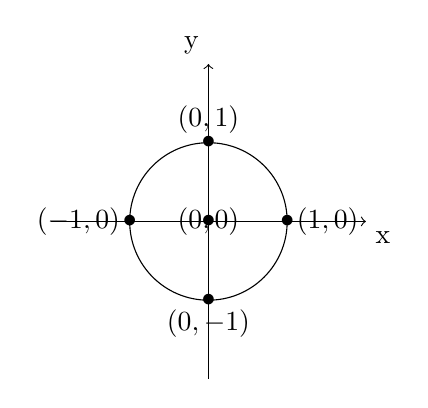
\begin{tikzpicture}
	\pgfmathsetmacro\MAX{2}
	\draw[->] (-\MAX,0) -- (\MAX,0) node[anchor=north west] {x};
	\draw[->] (0,-\MAX) -- (0,\MAX) node[anchor=south east] {y};
	\draw node at (0,0) {$(0,0)$};
	\draw node at (0,0) {$\bullet$};
	\draw node at (0,1) {$\bullet$};
	\draw node at (0,1) [anchor=south]{$(0,1)$};
	\draw node at (1,0) {$\bullet$};
	\draw node at (1,0) [anchor=west] {$(1,0)$};
	\draw node at (-1,0) {$\bullet$};
	\draw node at (-1,0) [anchor=east] {$(-1,0)$};
	\draw node at (0,-1) {$\bullet$};
	\draw node at (0,-1) [anchor=north]{$(0,-1)$};
	\draw (0,0) circle (1);
	\end{tikzpicture}\\
	Per prima cosa osservo che s possono trovare dei punti che rendono vera $f(x,y)=x^2+y^2-1=0$ e sono tutti i punti della circonferenza di centro l'origine degli assi e raggio unitario.\\
	il punto $(x_0,y_0)=(0,1)$ definisce implicitamente una funzione $y=\varphi(x)=\sqrt{1-x^2}$ con $\mathcal{X}=[-1,1]$ e $\mathcal{Y}=[0,1]$\\
	un primo problema \'e dovuto alla scelta degli intervalli $\mathcal{X},\mathcal{Y}$, per esempio posso scegliere $\mathcal{X}=[-\frac{1}{2},\frac{1}{2}]$ e $\mathcal{Y}=R^+$\\
	un secondo problema \'e la scelta del punto $(x_0,y_0)$, potrei scegliere il punto $(\frac{1}{\sqrt{2}},\frac{1}{\sqrt{2}})$\\
\observation
La stessa definizione pu\'o essere riscritta con la $x$ funzione della $y$ poich\'e a priori non c'\'e distinzione tra le variabili.
\proposition (caso lineare)\\
sia $f:R^n\times R^m\rightarrow R^p$ che $(x,y)\rightarrow Ax+By-C$ con $A\in Mat(p \times n), B\in (p \times m), B\in (p \times 1)$. Se $p=m$ cie\'e $B$ \'e un matrice quadrata, e $det(B)\ne 0$ cie\'e invertibile, allora\\
$\exists !\varphi : R^n\rightarrow R^m$ t.c.: $f(x,y)=0 \Leftrightarrow y=\varphi(x)$
\begin{proof}
	$f(x,y)=0\Leftrightarrow Ax+By=-C\Leftrightarrow By=-Ax+C\Leftrightarrow y=-B^{-1}Ax+B^{-1}C = \varphi(x)$
\end{proof}
\proposition
Sia $f:X\times Y\rightarrow R^m$ con $X\in R^n, Y\in R^m$\\
Preso un punto $(x_0,y_0)$ con $x_0\in \overset{\circ}{X}$,$y_0\in \overset{\circ}{Y}$\\
se:
\begin{enumerate}
	\item $f$ continua in $X\times Y$
	\item $f(x_0,y_0)=0$
	\item $f$ differenziabile rispetto a $y \forall (x,y)\in X\times Y$ e $D_yf(x,y)$ continua.
	\item $D_yf(x_0,y_0)$ invertibile .
\end{enumerate}
$\Rightarrow $ si ha:\\
esistenza della funzione implicita\\
$\exists \mathcal{X}\subseteq X$ intorno di $x_0$(xstrano aperto)\\
$\exists \mathcal{Y}\subseteq Y$ intorno di $y_0$(ystrano aperto)\\
$\exists\varphi$ continua con $\varphi:\mathcal{X}\rightarrow\mathcal{Y}$ t.c. $[\varphi (x_0)=y_0 e] f(x,y)=0, x\in\mathcal{X},y\in\mathcal{Y} \Leftrightarrow y=\varphi(x)$
unicit\'a di sostanza cio\'e a meno del dominio:\\
se $\varphi_i:\mathcal{X}_i\rightarrow\mathcal{Y}_i$ e $x_0\in\mathcal{X}_i,y_0\in\mathcal{Y}_i$\\
$f(x_0,y_0)=0 \forall x\in\mathcal{X}_i, y\in \mathcal{Y}\Leftrightarrow y=\varphi_i(x)$ con $i=1,2$\\
Allora $\forall\in\mathcal{X}\cap\mathcal{X}_1\cap\mathcal{X}_2$ vale $\varphi_1(x)=\varphi_2(x)$

\observation
Le ipotesi 3 e 4 garantiscono che esiste una approssimazione lineare, l'ipotesi 4 \'e sensata poiche $y$ e $f$ hanno lo stesso numero di componenti quindi $Dyf$ \'e un matrice qudrata.\\
la funzione $f:X\times Y\rightarrow R^m$ che $(x,y)\rightarrow f(x,y)$ ??????\\
cio\'e $\forall x\in X$ (sto fissando una x) $f^x:Y\rightarrow R^m$ che $y\rightarrow f(x,y)$(sto variando la y), $Df^x\in Mat(m\times m)$

\observation Metodo degli zeri di Newton per troare gli zeri di una funzione o metofo delle tangenti.\\
\resizebox {\columnwidth} {!} {
\begin{tikzpicture}
\draw[->] (-1,0) -- (5,0) node[anchor=north west] {y};
\draw[->] (0,-1) -- (0,4) node[anchor=south east] {z};
\draw[domain=-1:4,smooth,variable=\x,blue] plot ({\x},{(1/8)*(\x*\x)-(\x)+1.9});
\end{tikzpicture}
}\\
Scelgo un punto $y_0$ ne prendo il valore sulla curva, disegno la tangente e chiamo $y_1$ l'intersezione con l'asse $y$. Itero il processo $y_n+1=y_n\frac{f(y_n)}{f^{'}(y_n)}$\\
discorso al momento difficile per me....\\
\begin{proof}
	Dobbiamo partire da $f(x,y)=0$ arrivare a $y=\varphi(x)$,vogliamo applicare un raginamento simile a quello della Metodo di Newton, passando per\'o per il concetto di punto fisso, il teorema delle Contrazioni ci assicura che esiste unico.\\
	cerchiamo quindi una contrazione $T$ il cui punto fisso sia soluzione di $f(x,y)=0$. $T$ \'e del tipo:\\
	$T:?\times ?\rightarrow ?$\\
	$(x,y)\rightarrow y-[D_yf(X_0,y_0)]^{-1}f(x,y)$, nota che non avere nella derivata lo stesso punto in cui si calcola la funzione (come \'e nel metodo di Newton) ha effetti "tragici" sulla velocit\'a di convergenza, ma a noi interessa l'esistenza.\\
	bisgna capire quali insiemi usare come insiemi di partenza e arrivo, devo essere scelti in modo da poter applicare il teoremma delle contrazioni. Bisogna scegliere sottoinsiemi di $R^n$ e $R^m$, scegliamo quindi delle sfere\\
	$T:\overline{B(x_0,r_x)}\times\overline{B(y_0,r_y)}\rightarrow\overline{B(y_0,r_y)}$, scegliendo la chiusura delle sfere si è sicuri di lavorare in uno spazio metrico completo, poich\'e in $R^l$ completo $\Leftrightarrow$ chiuso e limitato.\\
	come vengono invece scelti i raggi? sono scelti in modo che:\\
	\begin{enumerate}
		\item $T$ \'e ben definita
		\item $\forall x \in \overline{B(x_0,r_x)} Tx: \overline{B(x_0,r_x)}\rightarrow\overline{B(y_0,r_y)}$ che $y\rightarrow T(x,y)$,\\
	\end{enumerate}
	cio\'e $T$ \'e una contrazione tale che $\forall x$ esiste un punto fisso, $\forall x$ associo a $y$ una x, e quindi na funzione.\\
	$r_x,r_y$ devono essere sufficientemene piccoli per avere tali propriet\'a e per poterci lavorare sopra.\\
	Abbiamo che $f(x,y)=0 \Leftrightarrow T(x,y)=y$\\
	$T(x,y)=y\Leftrightarrow y=y-[D_yF(x_0,y_0)]^{-1}f(x,y)$\\
	$[D_yF(x_0,y_0)]^{-1}f(x,y)\Leftrightarrow f(x,y)=0$\\
	Per verificare che $T$ \'e una contrazione ne stimo la norma\\
	$\left\| T(x,y_2)-T(x,y_1) \right\| \le \sup\limits_{\widetilde{y}\in segmento}\left\| D_yT(x,\widetilde{y})\right\|\left\| y_2-y_1 \right\| $  accrescimenti finiti.\\
	Poichè le sfere sono insiemi convessi \'e stato possibile applicare il Teorema degli accresscimenti finiti.\\
	Presa $T(x,y) = y-[D_yf(x_0,y_0)]^{-1}f(x,y)$, la derivo rispetto a $y$:
	$$D_yT(x,y)= I_{R^m}-[D_yf(x_0,y_0)]^{-1}D_yf(x,y) = $$
	$$=[D_yf(x_0,y_0)]^{-1}][D_yf(x_0,y_0)-D_yf(x,y)]$$
	Osserviamo che abbiamo ottenuto una matrice come costante moltiplicativa, al secondo membro abbiamo la differenza di due valori di una funzione, che per ipotesi \'e una funzione continua ($D_yf(x,y)$ continua), allora per $r_x$ e $r_y$ sufficientemente piccoli ho che:\\
	$\left\| D_yT(x,y) \right\| \le \frac{1}{2}$, \'e scelto questo valore poich\'e \'e comodo al fine di dimostrare la contrazione...\\
	$$\left\| D_yT(x,y)\right\| \le \left\| D_yf(x_0,y_0)]^{-1}\right\| \left\| D_yf(x_0,y_0)-D_yf(x,y)\right\|\le\frac{1}{2} $$  
	$$\left\| T(x,y_2)-T(x,y_1)\right\|\le\frac{1}{2}\left\|y_2-y_1\right\| $$
	Se dimostriamo che $T$ \'e ben definita abbiamo dimostrato che $T$ \'e una contrazione.\\
	Per verificare che $T$ \'e en definita bisogna mostrare che $T(x,y)\subseteq\overline{B(y_0,r_y)}$ quindi si mostra che la distanza tra $T(x,y)$ e il centro \'e minore di $r_y$
	$$\left\| T(x,y) - y_0\right\|\le\left\| T(x,y)-T(x,y_0)\right\|+\left\|T(x,y_0)-y_0\right\| \le$$
	$$\le\frac{1}{2}\left\|y-y_0\right\|+\left\|y_0-[D_yf(x_0,y_0)]^{-1}f(x,y_0)-y_0\right\|\le$$
	$$\le\frac{1}{2}\left\|y-y_0\right\|+\left\|[D_yf(x_0,y_0)]^{-1}\right\| \left\|f(x,y_0)-0\right\|\le$$
	$$\le\frac{1}{2}\left\|y-y_0\right\|+\left\|[D_yf(x_0,y_0)]^{-1}\right\| \left\|f(x,y_0)-f(x_0,y_0)\right\|\le$$
	$$\le\frac{1}{2}r_y+\frac{1}{2}r_y\le r_y$$
	Allora $T$ \'e ben definita perch\'e $T(x,y)\in\overline{B(y_0,r_y)}$.\\
	In conclusione con $\mathcal{X}=\overline{B(x_0,r_x)}$ e $\mathcal{Y}=\overline{B(y_0,r_y)}$ ho che $T:\mathcal{X}\times\mathcal{Y}\rightarrow\mathcal{Y}$ \'e tale che $\forall x\in\mathcal{X}$ la funzione $y\rightarrow T(x,y)$ \'e una contrazione e $\overline{B(y_0,r_y)}$ \'e completo.\\
	quaolcosa sui completi.........\\
	................................\\
	..........................\\
	A questo punto pu\'o essere applicato il teorema delle contrazioni:\\
	$\forall x \in \mathcal{X}, \exists y \in\mathcal{Y}: f(x,y)=0$ allora chiamo $\varphi:\mathcal{X}\rightarrow\mathcal{Y}$ che $x\rightarrow y$ \'e unica quindi $\varphi$ \'e una funzione.\\
	Allora la funzione implicita esiste. La continuit\'a direva direttamente dal teorema delle contrazioni: l'applicazione che al parametro associa il punto fisso \'e continua.\\
	Per l'unicit\'a si osservano le ipotesi 1 e 2, dove \'e scritto $\forall x$ ovvero scelta una qualunque $x$ la $y$ \'e unica quindi $\varphi$ \'e univocamente definita.
	  
\end{proof}
\proposition
Sia $f:X\times Y\rightarrow R^m$ con $X\in R^n, Y\in R^m$\\
Preso un punto $(x_0,y_0)$ con $x_0\in \overset{\circ}{X}$,$y_0\in \overset{\circ}{Y}$\\
se:
\begin{enumerate}
	\item $f(x_0,y_0)=0$
	\item $f\in C^1(X\times Y,R^m)$.
	\item $D_yf(x_0,y_0)$ invertibile .
\end{enumerate}
$\Rightarrow $ si ha:\\
\begin{enumerate}
	\item $\exists \varphi: \mathcal{X}\rightarrow\mathcal{Y}$ definita implicitamente da $f(x_0,y_0)=0$
	\item $\varphi$ continua su $\mathcal{X}$
	\item $\varphi$ \'e differenziabile e $D\varphi(x)=-[D_yf(x,\varphi(x))]^{-1}D_xf(x,\varphi(x))$
\end{enumerate}
\begin{proof}
	I punti 1 e 2 sono gli stessi del teorema della funzione implicita e si dimostrano allo stesso modo.\\
	Per il punto 3 abbiamo che $f(x,y)=0\Leftrightarrow y=\varphi(x)$ e quindi $\forall x\in \mathcal{X}$ $f(x,\varphi(x))=0$\\
	.........\\
	.........\\
	
\end{proof}

\proposition CASO N=1, M=1\\
Sia $f:X\times Y\rightarrow R$ con $X\in R, Y\in R$\\
Preso un punto $(x_0,y_0)$ con $x_0\in \overset{\circ}{X}$,$y_0\in \overset{\circ}{Y}$\\
se:
\begin{enumerate}
	\item $f(x_0,y_0)=0$
	\item $f\in C^1(X\times Y,R)$.
	\item $\partial_yf(x_0,y_0)\ne 0$.
\end{enumerate}
$\Rightarrow $ si ha:\\
\begin{enumerate}
	\item $\exists \varphi: \mathcal{X}\rightarrow\mathcal{Y}$ definita implicitamente da $f(x_0,y_0)=0$
	\item $\varphi\in C^0(\mathcal{X},\mathcal{Y})$
	\item $\varphi$ \'e derivabile e $\varphi^{'}(x)=-[\partial_yf(x,\varphi(x))]^{-1}\partial_xf(x,\varphi(x))$
\end{enumerate}
\begin{proof}
	$f(x,y)=0\Leftrightarrow y=\varphi(x)$, derivando $D(f(x,\varphi(x)))=0$\\
	$\partial_xf(x,\varphi(x))+\partial_yf(x,\varphi(x))\varphi^{'}(x)=0$\\
	allora $\varphi^{'}(x) = -\frac{\partial_xf(x,\varphi(x))}{\partial_yf(x,\varphi(x))}$
\end{proof}
\observation Non essendoci motivo per preferire la $x$ alla $y$ o viceversa, esiste anche una versione di questo teorema  in  cui le ipotesi sono le stesse eccetto l'ultima che diventa $\partial_xf(x_0,y_0)\ne 0$
\begin{enumerate}
	\item $\exists \psi: \mathcal{Y}\rightarrow\mathcal{X}$ definita implicitamente da $f(x,y)=0$
	\item $\psi\in C^0(\mathcal{Y},\mathcal{X})$
	\item $\psi$ \'e derivabile e $\psi^{'}(y)=-[\partial_xf(\psi(y),y)]^{-1}\partial_yf(\psi(y),y)$
\end{enumerate}
Qualche esempio qui\\
\section{Il Teorema della funzione Inversa}
Data una funzione f, poterla invertire  ...... unico modo l'equazione (o sistema ....)... l'incognita $x$ in funzione del parametro .....\\
\proposition(Teorema della funzione inversa caso lineare)\\
Sia $f:R^n\in R^m$ data da $f(x)=Mx$ e $M\in Mat(m\times n)$, $f$ \'e invertibile $\Leftrightarrow n=m$ e $detM\ne 0$
\proposition(caso generale)\\
sia $f:A\rightarrow R^n$ con $A\in R^n$, $f\in C^1(A,R^n)$, $x_0\in \overset{\circ}A$ e $Df(x_0)$ invertibile.\\
Allora $\exists\mathcal{X}\in A,\exists\mathcal{Y}\in R^n$, $\exists\varphi\mathcal{Y}\rightarrow\mathcal{X}$ con la propriet\'a $f(x)=y\Leftrightarrow x=\varphi(y)$ con $x\in\overset{\circ}{\mathcal{X}}$ e $y\in\overset{\circ}{\mathcal{Y}}$ e $\varphi\in C^1(\mathcal{Y},\mathcal{X})$ e $D\varphi(y)=[Df(x)]^{-1}$\\
\begin{proof}
	$f(x)=y\Leftrightarrow f(x)-y=0$. Allora introduco $F:A\times R^n\rightarrow R^n$ data da $F(x,y)=f(x)-y$.\\
	Studio $F(x,y)=0$ per ottenere $x=\varphi(y)$.\\
	Per poter applicare il teorema della funzione implicita serve $D_xF(x_0,y_0)$ invertibile, ma $D_xF(x_0,y_0)=Df(x_0)$ che \'e invertibile per ipotesi.\\
	Applico allora il teorema della funzione implicita , quindi gli intorni esistono e $x=\varphi(y)$.\\
	resta da trovare la derivata totale di $\varphi$. Sappiamo che $f\in C^1$ quindi $\varphi \in C^1$.\\
	Sappiamo che $\varphi(f(x))=x$, applicando la derivata della funzione composta abbiamo che:\\
	$D\varphi(f(x))Df(x)=I$\\
	$D\varphi=[Df(x)]^{-1}$ quando $\varphi(y)=x$\\
	si puo anche scrivere come $(Df^{-1})(f(x))=[Df(x)]^{-1}$
\end{proof}
\section{Massimi e Minimi Liberi}
\definition
Siano $(X,d)$s.m., $A\subseteq X$ e $f:A\rightarrow R$, siano $x_0\in A, B\in A$ e $m,M\in R$ ( L'insieme immagini deve essere $R$ per poter parlare di massimi e minimi, $R$ \'e un campo ordinato a differenza di $R^n$).\\
$M$ \'e massimo di $f$ su $B \rightleftharpoons M=\max f(B)\Leftrightarrow\forall x \in B f(x_0)\ge f(x)$\\
$M$ \'e minimo di $f$ su $B \rightleftharpoons m=\min f(B)\Leftrightarrow\forall x \in B f(x_0)\le f(x)$\\
$x_0$ \'e punto di massimo assoluto per $f \rightleftharpoons f(x_0)=\max\limits_{A}f(x)$\\
$x_0$ \'e punto di minimo assoluto per $f \rightleftharpoons f(x_0)=\min\limits_{A}f(x)$\\
$x_0$ \'e punto di massimo locale relativo per $f \rightleftharpoons \exists r>0: f(x_0)=\max\limits_{x\in B(x_0,r)}f(x)$ con $B(x_0,r)\subseteq A$\\
$x_0$ \'e punto di minimo locale relativo per $f \rightleftharpoons \exists r>0: f(x_0)=\min\limits_{x\in B(x_0,r)}f(x)$ con $B(x_0,r)\subseteq A$\\
\subsection{Condizioni Necessarie}
\proposition{Teorema di Fermat}\\
sia $f:A\subseteq R^n\rightarrow R$ e $x_0\in\overset{\circ}A$. Se $x_0$ \'e punto di massimo(0 minimo) locale per $f$ su $A$ e $f$ \'e differenziabile in $x_0$ allora $\nabla f(x_0)=0$.
\begin{proof}
	Sia $v\in R^n$ con $\left\| v\right\| =1$, la funzione $F(t)= f(x_0+tv)$ che a $t\rightarrow x_0+tv$ \'e il moto rettilineo uniforme che passa da $x_0$ all'istante $0$ e si muove con velocit\'a vettore costante $v$. Cio\'e per tempi negativi mi avvicino a $x_0$ al tempo zero si \'e in $x_0$ e per tempi positivi si allontana da $x_0$. quindi $t=0$ \'e punto di massimo per $F$, allora $F^{'}(0) = 0$ per il teorema di Fermat di A1.\\
	Ora abbiamo che $F^{'}(t)=\nabla f(x_0+tv)v$ quindi $F^{'}(0)=\nabla f(x_0)v$ cio\'e $\nabla f(x_0)v=0$.\\
	Quindi $\forall v :\left\| v\right\| =1$ vale $\nabla f(x_0)=0$\\
	OSS:: Vale anche che $D_vf(x_0)=0$
\end{proof}
\definition
sia $f:A\subseteq r^n\rightarrow R$, $x_0\in\overset{\circ}{A}$\\
$x_0$ \'e punto stazionario .... $\rightleftharpoons$ $f$ \'e differenziabile in $x_0$ e $\nabla f($ ......
\observation
nel caso $n=2, m=1, \nabla f(x_0,y_0)=[\partial_xf(x_0,y_0), \partial_yf(x_0,y_0)]$ ..... i punti stazionari sono quelli che ......parziali.
\observation
Prima di continuare un paio di osservazioni sulle forme quadratiche.\\
\definition
forma quadratica su $R^n \rightleftharpoons q:R^n\rightarrow R$ che $x\rightarrow x^TQx$ con $Q\in Mat(n\times n)$ simmetrica\\
ESEMPI:n=2\\
$$
Q=\begin{bmatrix}1&&0\\0&&1\end{bmatrix}\quad
Q=\begin{bmatrix}-1&&0\\0&&-1\end{bmatrix}\quad
Q=\begin{bmatrix}-1&&0\\0&&1\end{bmatrix}\quad 
$$
SEMPRE POSITIVA SEMPRE NEGATIVA CAMBIA SEGNO\\
SEMPRE POSITIVA SEMPRE NEGATIVA CAMBIA SEGNO\\
SEMPRE POSITIVA SEMPRE NEGATIVA CAMBIA SEGNO\\
\proposition
se $Q$ \'e una forma quadratica, allora\\
\begin{itemize}
	\item $\forall\lambda\in R, \forall x\in R^n$ $q(\lambda x)=\lambda^2q(x)$
	\item $q(0)=0$
	\item se $q$ \'e limitata $\Rightarrow q\equiv 0$ 
\end{itemize}
\begin{proof}
	\begin{itemize}
		\item $q(\lambda x)=(\lambda x)^TQ(\lambda x)=\lambda^2x^TQx=\lambda^2q(x)$
		\item $q(0)=q(0x)=0q(x)=0$
		\item (contronominale $q\ne 0 \Rightarrow q$ non \'e limitata).\\
		se $q$ \'e non nulla $\Rightarrow \exists x \in R^n$ $q(x)\ne 0$\\
		allora $q(\lambda x)=\lambda^2q(x)$ illimitata.
		\item ???????????????????????????????????????????????
	\end{itemize}
\end{proof}
\proposition
se $q$ \'e una forma quadratica $\Rightarrow\exists M\ge 0: |q(x)|\le M\left\| x \right\|^2$ $\forall x\in R^n$
\begin{proof}
	per $x\ne 0$ $\left| q(x)\right| =\left| q\left(\left\| x\right\| \frac{1}{\left\| x\right\| }x\right) \right| = \left\|x\right\|^2\left|q\left(\frac{1}{\left\|x\right\|}x\right)\right|\le$\\
	$\le\left(\sup\limits_{\left\|x\right\|=1}\left|q(x)\right|\right)\left\|x\right\|^2=\le\left(\max\limits_{\left\|x\right\|=1}\left|q(x)\right|\right)\left\|x\right\|^2=M\left\|x\right\|^2$
\end{proof}
\proposition
Sia $q$ una forma quadratica, se $q(x)=o(\left\|x\right\|^2)$ per $x\rightarrow 0 \Rightarrow q\equiv 0$
\begin{proof}
	sia $x\in R^n$ con $\left\|x\right\|=1$ e $t>0$.\\
	$q(x)=\frac{1}{t^2}$, $q(tx)=\frac{q(tx)}{\left\|tx\right\|^2}\rightarrow 0$ per $t\rightarrow 0$ per ipotesi.\\
	Allora $\forall x$ con $\left\|x\right\|$ vale $q(x)=0$ e allora $\forall x\ne 0, q(x)=q\left(\frac{1}{\left\|x\right\|}x\right)\left\|x\right\|^2$
\end{proof}
\definition
Sia $q:R^n\rightarrow R$ una forma quadratica\\
\begin{itemize}
	\item $q$ \'e definita positiva $\rightleftharpoons \forall x\in R^n, x\ne 0$ $q(x)>0 [Q>0]$
	\item $q$ \'e semidefinita positiva $\rightleftharpoons \forall x\in R^n$ $q(x)\ge0 [Q\ge0]$
	\item $q$ \'e definita negativa $\rightleftharpoons \forall x\in R^n, x\ne 0$ $q(x)<0 [Q><0]$
	\item $q$ \'e semidefinita negativa $\rightleftharpoons \forall x\in R^n$ $q(x)\le0 [Q\le0]$
\end{itemize}
\proposition
Sia $q:R^n\rightarrow R$ una forma quadratica, se $q$ \'e definita positiva $\Rightarrow \exists m>0: \forall x \in R^n, q(x)\ge m\left\|x\right\|^2$
\begin{proof}
	Noto che $q(\lambda x)=\lambda^2q(x)$\\
	$q(x)=q\left(\frac{1}{\left\|x\right\|}x\left\|x\right\|^2\right)\ge\min\limits_{\left\|x\right\|=1}q(\lambda)\left\|x\right\|^2$
\end{proof}
Ora dobbiamo cercare di capire se $q$ \'e definita positiva\\
Ad esempio: $Q=\begin{bmatrix}1&&0&&0\\0&&-1&&0\\0&&0&&0\end{bmatrix}$ \'e facile capire che \'e semodefinita positiva poich\'e \'e in diagonale, quindi la prima cosa da fare \'e trovare una forma diagonale per $Q$\\
un procedimento pratico e veloce \'e il seguente:\\
$$Q=\begin{bmatrix}q_{11}&&q_{12}&&q_{13}&&\ldots\\q_{21}&&q_{22}&&q_{23}&&\ldots\\q_{31}&&q_{32}&&q_{33}&&\ldots\\\vdots&&\vdots&&\vdots&&\ddots\end{bmatrix}\rightarrow\begin{bmatrix}\lambda_{1}&&0&&0&&\ldots\\0&&\lambda_{2}&&0&&\ldots\\0&&0&&\lambda_{3}&&\ldots\\\vdots&&\vdots&&\vdots&&\ddots\end{bmatrix}$$
$$\lambda=q_{11},\quad\lambda_{2}=\frac{detQ_2}{q_11}\quad\lambda_{3}=\frac{detQ_3}{detQ_2}\quad ...\quad \lambda_{i}=\frac{detQ_i}{detQ_{i-1}}$$
Questo perch\'e se dobbiamo valutare il segno dell'incremento della f ci servono le variazioni sulle quadriche. Se $f$ \'e $C^2$ scrivo lo sviluppo di Taylor al secondo ordine:\\
$$f(x)-f(x_0)=\nabla f(x_0)(x-x_0)+\frac{1}{2}(x-x_0)^TH_f(x_0)(x-x_0)+o(\left\|x-x_0\right\|^2)$$
max e min dove $\nabla f(x_0)=0$ per Fermat, l'o piccolo \'e trascurabile, allora il segno della derivata dipende dalla forma quadratica al secondo membro.
\proposition
sia $f:A\subseteq R^n\rightarrow R$ e $x_0\in\overset{\circ}{A}$.\\
$f\in C^2(A;R)$ e $x_0$ punto di massimo locale per $f$ su $A\Rightarrow\nabla f(x_0)=0$ e $H_f(x_0)$ \'e semidefinita negativa.
\begin{proof}
	$f(x)-f(x_0)=\frac{1}{2}(x-x_0)^TH_f(x_0)(x-x_0)+o(\left\|x-x_0\right\|^2)$ poich\'e $f\in C^2$\\
	il primo termine \'e negativo poich\'e per ipotesi $x_0$ \'e punto di massimo locale, ne segue che il termine $(x-x_0)^TH_f(x_0)(x-x_0)$ non pu\'o essere positivo. 
\end{proof} 
\proposition
sia $f:A\subseteq R^n\rightarrow R$ e $x_0\in\overset{\circ}{A}$.\\
$f\in C^2(A;R)$ e $x_0$ punto di minimo locale per $f$ su $A\Rightarrow\nabla f(x_0)=0$ e $H_f(x_0)$ \'e semidefinita positiva.
\begin{proof}
	$f(x)-f(x_0)=\frac{1}{2}(x-x_0)^TH_f(x-x_0)+o(\left\|x-x_0\right\|^2)$ poich\'e $f\in C^2$\\
	il primo termine \'e positivo poich\'e per ipotesi $x_0$ \'e punto di minimo locale, ne segue che il termine $(x-x_0)^TH_f(x-x_0)$ non pu\'o essere negativo. 
\end{proof} 


\subsection{Condizioni Sufficienti}
\proposition
sia $f:A\subseteq R^n\rightarrow R$ e $x_0\in\overset{\circ}{A}$.\\
$f\in C^2(A;R)$, $\nabla f(x_0)=0$,$H_f(X_0)$ \'e definita negativa $\Rightarrow x_0$ \'e un punto di massimo locale per $f$
\begin{proof}
	$f\in C^2$ quindi possiamo scrivere:\\
	$f(x_+h)-f(x_0)=\nabla f(x_0)h+\frac{1}{2}(h)^TH_f(x_0)+o(\left\|h\right\|^2)$ per $h\rightarrow 0$\\
	$f(x_+h)-f(x_0)=\frac{1}{2}(h)^TH_f(x_0)+o(\left\|h\right\|^2)$ per $h\rightarrow 0$\\
	Sappiamo che $H_f$ \'e definita negativa per ipotesi, allora $h^TH_f(x_0)h\le -m\left\|x_0\right\|$ allora $f(x_0+h)-f(x_0)<0$ e quindi $x_0$ \'e punto di massimo locale per $f$.
\end{proof} 
\proposition
sia $f:A\subseteq R^n\rightarrow R$ e $x_0\in\overset{\circ}{A}$.\\
$f\in C^2(A;R)$, $\nabla f(x_0)=0$,$H_f(X_0)$ \'e definita positiva $\Rightarrow x_0$ \'e un punto di minimo locale per $f$
\begin{proof}
	$f\in C^2$ quindi possiamo scrivere:\\
	$f(x_+h)-f(x_0)=\nabla f(x_0)h+\frac{1}{2}(h)^TH_f(x_0)+o(\left\|h\right\|^2)$ per $h\rightarrow 0$\\
	...........\\
	...........\\
\end{proof} 
QUALCHE DISEGNO E SPIEGAZIONE.....
\subsection{Il Significato Geometrico del Gradiente n=2 m=1}
\definition
Sia $A\subseteq R^2$ e $f:A\rightarrow R$\\
La suferficie $z=f(x,y)$ \'e il grafico di $f$, \'e unsottoinsieme di $R^3$\\
Se $c\in R$, la curva di livello $c$ di $f$ \'e l'insieme $f^{-1}(c)\{(x,y)\in A: f(x,y)=c\}$\\
Se $f$ 	'e differenziabile in $(x_0,y_0)\in\overset{\circ}{A}$ il piano tangente alla superficie $z=f(x,y)$ in $(x_0,y_0)$ ha equazione:\\
$$z=f(x_0,y_0)+\nabla f(x_0,y_0)\begin{bmatrix}(x-x0)\\(y-y_0)\end{bmatrix}$$ 
$$z=f(x_0,y_0)+\partial_xf(x_0,y_0)(x-x_0)+\partial_yf(x_0,y_0)(y-y_0)$$
\observation
geometricamente, il gradiente di una funzione indica la direzione di $R^n$ in cui si ha la massima variazione del valore di f, nel verso di incremento positivo di $f$,
\observation 
osservazione col grafico che al momento non faccio.
\proposition
Siano $A\subseteq R^n, f:A\rightarrow R$ differenziabile in $(x_0,y_0)\in \overset{\circ}{A}$, l'incremento di $f(x_0+h,y_0+k)-f(x_0,y_0)$ \'e massimo quando $[h k]=\lambda\nabla f(x_0,y_0)$ con $\lambda >0$ ed \'e minimo con $[h k]=\lambda\nabla f(x_0,y_0)$ con $\lambda <0$
\begin{proof}
	so che posso approssimare la funzione quindi posso scrivere:\\
	$f(x_0+h,y_0+k)-f(x_0,y_0)=\nabla f(x_0,y_0)\begin{bmatrix}h\\k\end{bmatrix}+o(\sqrt{h^2+k^2})$=
	$=\left\| \nabla f(x_0,y_0) \right\|\left\|\begin{bmatrix}h k\end{bmatrix}\right\|cos(\theta)+o(\sqrt{h^2+k^2})$\\
	dove $\theta$ \'e l'angolo tra $\nabla f(x_0,y_0)$ e $[h k]$ per $||[h k]||$ sufficientemente piccola, l'incremento $f(x_0+h,y_0+k)-f(x_0,y_0)$ \'e massimo se $cos( \theta )=1$ ed \'e minimo se $cos(\theta )=-1$, da cui la tesi.\\ 
\end{proof}
\proposition
siano $f\in C^1(A;R)$ con $A\subseteq R^2$ e $(x_0,y_0)\in\overset{\circ}{A}$ e $\nabla f(x_0,y_0)\ne 0$[cie\'e stazionario]. Allora $nabla f(x_0,y_0)$ \'e perpendicolare alla curva di livello passante per .....
\observation
un vettore 1'e perpendicolare a una curva se \'e perpendicolare alla retta o al vettore tangente alla curva in quel punto.
\begin{proof}
	La curva di livello \'e $f(x,y)=f(x_0,y_0)$ cio\'e $f(x,y)-f(x_0,y_0)=0$, per trovare la tangente a questa curva \'e piu facile se si ha $y=\varphi(x)$\\
	Usiamo quindi il teorema della funzione implicita, mi serve che $\partial_yf(x_0,y_0)\ne 0$, questa condizione non \'e assicurata dalle ipotesi, per ipotesi il gradiente \'e non nulla quindi almeno una delle due componenti \'e non nulla.\\
	Inizio con il caso $\partial_yf(x_0,y_0)\ne 0$.\\
	Il T.F.IMPL. assicura che :\\
	$\exists\mathcal{X},\mathcal{Y}$ con $x_0\in\overset{\circ}{\mathcal{X}}, y_0\in\overset{\circ}{\mathcal{Y}}$, $\exists\varphi:\mathcal{X}\rightarrow\mathcal{Y}$ t.c.:\\
	$f(x,y)=f(x_0,y_0), x\in\mathcal{X}, y\in\mathcal{Y} \Leftrightarrow y=\varphi(x)$\\
	La retta tangente in $x_0$ a $y=\varphi(x)$ \'e $y=y_0+\varphi^{'}(x_0)(x-x_0)$\\
	questo vuole dire che un vettore tangente a $y=\varphi(x)$ in $(x_0,y_0)$ \'e $\begin{bmatrix}1\\\varphi^{'}(x_0)\end{bmatrix}$.\\
	... calcolo il prodotto scalare\\
	$$\nabla f(x_0,y_0)\begin{bmatrix}1\\\varphi^{'}(x_0)\end{bmatrix} = \begin{bmatrix}\partial_x f(x_0,y_0)&&\partial_y f(x_0,y_0)\end{bmatrix}\begin{bmatrix}1\\-\frac{\partial_x f(x_0,y_0)}{\partial_y f(x_0,y_0)}\end{bmatrix} =$$ 
	$$=\partial_x f(x_0,y_0) -\partial_y f(x_0,y_0)\frac{\partial_x f(x_0,y_0)}{\partial_y f(x_0,y_0)}=0$$
	Allora il graadiente \'e perpendicolare alla curva di livello.\\
	Guardiamo ora al caso in cui $\partial_yf(x_0,y_0)= 0$ e $\partial_xf(x_0,y_0)\ne 0$ quindi il gradiente \'e non nullo.\\
	Applicando lo stesso ragionamento id sopra, solo esplicitando la $x$ in funzione della $y$. Quindi $x=\psi(x)$ e $\psi{'}(y_0)=-\frac{\partial_y f(x_0,y_0)}{\partial_x f(x_0,y_0)}$
\end{proof}

\section{Massimi e Minimi Vincolati}
Spesso la ricerca di punti di massimo o minimo di una funzione $f:A\rightarrow R, A\subseteq R^n$ deve essere ristrettaad un sottoinsieme $B\subseteq A$ a causa di eventuali vincoli a cui le variabili indipendenti devono soddisfare. L0insieme $B$ pu\'o essere generalmente descritto da una funzione $\varphi :A\rightarrow R^p$, nel senso che $B=\{x\in A:\varphi (x)\le 0\}$\\
NOTA::: direi n>1 poiche se ho una sola variabile e la vincolo ...??????? booooo .\\
Questo problema \'e usualmente abbreviato in:
$$\max\limits_{\varphi \le 0}\quad o \quad\min\limits_{\varphi \le 0}$$
pu\'o essere affrontato in due passi:\\
\begin{enumerate}
	\item ricerca dei punti di estremo di $f$ interni a $B$, problema gia affrontato.
	\item ricerca dei punti di estremo di $f$ sul bordo di $B$, affrontiamo ora.
\end{enumerate}
Sotto opportune condizioni su $\varphi$, infatti, $\overset{\circ}{B} = \{x\in A:\varphi(x)<0\}$ e $\partial B\{x\in A:\varphi(x)=0\}$
\proposition{Teorema dei Moltiplicatori di Lagrange}
Siano $f,g:A\subseteq R^2\rightarrow R, (x_0,y_0)\in\overset{\circ}{A}, g(x_0,y_0)=0, f,g\in C^1(A;R)$, $\nabla g (x_0,y_0)\ne 0$\\
Se $(x_0,y_0)$ \'e di max(o min) locale per $f$ su $g=0\Rightarrow\exists \lambda in R$ t.c: $\nabla f(x_0,y_0) = \lambda g(x_0,y_0)$ (all fin fine posso dire che sono paralleli).\\
\observation
$\lambda$ si chiama "moltiplicatore di lagrange"
\observation
Se abbiamo un problema del tipo $\max\limits_{g(x,y)=0}f$ cio\'e il massimo di $f$ sul vincolo $g(x,y)=0$, ci dobbiamo ricondurre ad un sistema del tipo
$\begin{cases} \nabla f(x_0,y_0)=\lambda \nabla g(x_0,y_0)\\ g(x_0,y_0)=0 \end{cases}=\begin{cases} \partial_xf(x_0,y_0)=\lambda \partial_xg(x_0,y_0)\\\partial_yf(x_0,y_0)=\lambda \partial_yg(x_0,y_0)\\ g(x_0,y_0)=0 \end{cases}$\\
3 equazioni in 3 incognite($x,y,\lambda$)\\
In certi casi si introduce una funzione $\mathcal{L}(x,y,\lambda) = f(x,y)-\lambda g(x,y)$ detta Lagrangiana, i punti stazionari vincolati di $f$ sono punti stazonari liberi della Lagrangiana.\\
\begin{proof}
	Sappiamo che $\nabla g(x_0,y_0)\ne$ quindi $\begin{bmatrix}\partial_xg(x_0,y_0) &&\partial_yg(x_0,y_0)\end{bmatrix}\ne\begin{bmatrix}0&&0\end{bmatrix}$ quindi o $\partial_xg(x_0,y_0)\ne 0$ o $\partial_yg(x_0,y_0)\ne 0$.
	Mettiamoci nel caso in cui $\partial_yg(x_0,y_0)\ne 0$,\\
    Per il teorema della funzione implicita ho che :\\
	$\exists\mathcal{X},\mathcal{Y}$ con $x_0\in\overset{\circ}{\mathcal{X}}, y_0\in\overset{\circ}{\mathcal{Y}}$, $\exists\varphi:\mathcal{X}\rightarrow\mathcal{Y}$ t.c.:\\
	$g(x,y)=f(x_0,y_0), x\in\mathcal{X}, y\in\mathcal{Y} \Leftrightarrow y=\varphi(x)$\\
	Osserviamo che dire $(x_0,y_0)$ di massimo o minimo per $f$ ristretta a $g(x,y)=0\Leftrightarrow x_0$ \'e di massimo o di minimo per la funzione $x\rightarrow f(x,\varphi(x))$.\\
	Per il teorema di Fermat $\left.\frac{d}{dx}(f(x,\varphi(x)))\right\|_{x=x_0}=0$, punto stazionario ha derivata nulla, e la derivata di quella funzione in $x_0$ \'e:
	$$\partial_xf(x_0,\varphi(x_0))+\partial_yf(x_0,\varphi(x_0))\cdot\varphi^{'}(x_0)$$ 
	allora
	$$0=\partial_xf(x_0,\varphi(x_0))+\partial_yf(x_0,\varphi(x_0))\cdot\varphi^{'}(x_0)=$$
	$$=\partial_xf(x_0,\varphi(x_0))-\partial_yf(x_0,\varphi(x_0))\frac{\partial_xg(x_0,\varphi(x_0))}{\partial_yg(x_0,\varphi(x_0))}=$$\\
	$$=\partial_xf(x_0,\varphi(x_0))\partial_yg(x_0,\varphi(x_0))-\partial_yf(x_0,\varphi(x_0))\partial_xg(x_0,\varphi(x_0))=det\left(\begin{matrix}\partial_xf(x_0,y_0)&&\partial_yf(x_0,y_0)\\\partial_xg(x_0,y_0)&&\partial_yg(x_0,y_0)\end{matrix}\right)=0$$\\
	questo equivale a dire che i vettori riga della matrice sono paralleli quindi $\exists\alpha\in R : \nabla f(x_0,y_0)=\lambda\nabla g(x_0,y_0)$.\\
	Non \'e uguale scrivere $\exists\alpha\in R : \nabla g(x_0,y_0)=\lambda\nabla f(x_0,y_0)$ poiche non c'\'e certezza sul valore di $\nabla f(x_0,y_0)$ che se nullo negherebbe l'ipotesi di $\nabla g(x_0,y_0)\ne 0$\\
	Se guardiamo ora il caso in cui $\partial_yg(x_0,y_0)=0$ e $\partial_xg(x_0,y_0)\ne 0$.\\
	Seguendo un ragionamento analogo si esplicita $x=\psi(y)$ cos\'i che cercare max(o min) di $f$ ristretta a $g(x,y)=0$ porti a $y\rightarrow f(\psi(y),y)$ 
\end{proof}
\proposition{Teorema dei Moltiplicatori di Lagrange caso generale}
Sia $A\in R^n$, $f\in C^1(A;R)$, $g\in C^1(A;R^p)$ con $p<n$(n.vincoli<n.variabili), sia poi $x_0\in\overset{\circ}{A}, g(x_0)=0, Dg (x_0,y_0)$ di rango $p$.\\
Se $x_0$ \'e di max(o min) locale per $f$ su $g=0\Rightarrow\exists \lambda_1,\ldots,\lambda_p in R$ t.c: $\nabla f(x_0,y_0) = \sum\limits_{i=1}^{p}\lambda_i\nabla g(x_0,y_0)$\\
\section{Derivate e Integrali}
\proposition{Teorema Fondamentale del Calcolo Integrale}
Sia $I\subseteq R$ un intervallo e sia $x_0\in I$. Data $f\in c^0(I;R)$ la funzione:\\
$\begin{array}{rcl} F: I & \to & R \\ x & \to & \int_{x_0}^{x}f(t)dt \end{array}$\\
Si ha $F\in C^1(I;R)$ e $F^{'}(x)=f(x)$ $\forall x \in I$
\proposition
Sia $A\subseteq R^n$ un aperto, data $f\in C^0(A\times R;R)$ la funzione \\
$\begin{array}{rcl} F: R\times R\times A & \to & R \\ (\alpha,\beta,x) & \to & \int_{\alpha}^{\beta}f(x,t)dt \end{array}$\\
\'e di classe $C^0(R\times R\times A;R)$
\proposition
Sia $A\subseteq R^n$ un aperto, data $f\in C^1(A\times R;R)$ la funzione \\
$\begin{array}{rcl} F: R\times R\times A & \to & R \\ (\alpha,\beta,x) & \to & \int_{\alpha}^{\beta}f(x,t)dt \end{array}$\\
\'e di classe $C^1(R\times R\times A;R)$ ed inoltre, $\forall (\alpha,\beta,x)\in R\times R\times A$ e $\forall i=1,\ldots,n$\\
$$\frac{\partial F}{\partial \alpha}=-f(x,\alpha)$$
$$\frac{\partial F}{\partial \beta}=f(x,\beta)$$
$$\frac{\partial F}{\partial x_i}=\int_{\alpha}^{\beta}\frac{\partial F}{\partial x_i}(x,t)dt$$
$$\nabla F=\int_{\alpha}^{\beta}\nabla f(x,t)dt$$
\corollary
Sia $A\subseteq R^n$ un aperto, date le funzioni $\alpha:x\rightarrow R, \beta:x\rightarrow R, f:x\rightarrow R, $ di classe $C^1$ , la funzione \\
$\begin{array}{rcl} F: A & \to & R \\ (x) & \to & \int_{\alpha(x)}^{\beta(x)}f(x,t)dt \end{array}$\\
\'e di classe $C^1(R\times R\times A;R)$ ed inoltre, $\forall x_0 \in A$:
$$\nabla F(x_0,y_0)=f(x_0,\beta)\nabla\beta(x_0)-f(x_0,\alpha)\nabla\alpha(x_0)+\int_{\alpha(x_0)}^{\beta(x_0)}\nabla f(x,t)dt$$



\part{Integrali Doppi}
\chapter{Integrali Doppi}
\section{Preliminari}
Questo capitolo non è trattato in maniera approfondita poiché:
\begin{description}
	\item[a] tanti e lunghi teoremi fuori contesto per poter introdurre rigorosamente la teoria di Riemann
	\item[b] tale teoria è "superata" da tempo
\end{description}
Il primo è più grosso problema di tale teoria è che non permette il passaggio del limite sotto il segno di integrale, cioè per poter scrivere 
$$ \int\lim\limits_{n\to\infty}f_n(x) = \lim\limits_{n\to\infty}\int f_n(x)$$ sono necessarie tante ipotesi molto restrittive.\\
Si è passati così alla teoria dell'integrale secondo Lebesgue, molto diversa e piuttosto complicata.\\
ESEMPIO...............\\
disegni...........\\
................\\
Il concetto di integrale è quindi molto legato al concetto di area e anche di volume. La teoria di Lebesgue riparte da assiomi come questi definendoli e caratterizzandoli in modo da definire una volta per tutte in maniera sistematica e rigorosa cosa si può e cosa non si può integrare, e dove ha senso parlare di superfici. volumi, ipervolumi, ... 
\section{Regole di Calcolo}
Queste formule permettono di ricondurre il calcolo di integrali doppi a quello di integrali semplici.\\
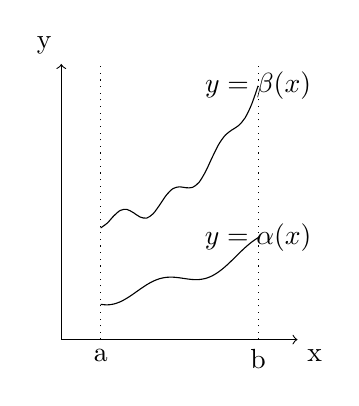
\begin{tikzpicture}
\draw[->] (0,0) -- (3,0) node[anchor=north west] {x};
\draw[->] (0,0) -- (0,3.5) node[anchor=south east] {y};
\draw[dotted] (.5,0) -- (.5,3.5);
\draw[dotted] (2.5,0) -- (2.5,3.5);
\draw (.5,0)  node[anchor=north] {a};
\draw (2.5,0) node[anchor=north] {b};
\draw[domain=.5:2.5,smooth,variable=\x] plot ({\x},{(1/9)*\x*\x*\x+1.5+0.1*sin(10*\x r)}) node {$y=\beta(x)$};
\draw[domain=.5:2.5,smooth,variable=\x] plot ({\x},{(1/9)*\x*\x+0.5+0.1*cos(5*\x r)}) node {$y=\alpha(x)$};
\end{tikzpicture}\\
Se:\\
$a,b\in \R$ con $a<b$\\
$\alpha,\beta\in C^0([a,b];R), \forall x\in[a,b] \alpha(x)\le\beta(x)$\\
$A=\{(x,y)\in \R^2: x\in [a,b] $e$ y\in [\alpha(x),\beta(x)] \}$\\
$f\in C^0(A;R)$\\
Allora\\
$\iint_Af(x,y)dxdy=\int_a^b\left(\int_{\alpha(x)}^{\beta{x}}f(x,y)dy\right)dx$\\
Analogamente.\\
ALTRO GRAFICO....\\
Se:\\
$c,d\in \R$ con $c<d$\\
$\gamma,\delta\in C^0([a,b];R), \forall y\in[c,d] \gamma(y)\le\delta(y)$\\
$A=\{(x,y)\in \R^2: x\in [c,d] $e$ x\in [\gamma(y),\delta(y)] \}$\\
$f\in C^0(A;R)$\\
Allora\\
$\iint_Af(x,y)dxdy=\int_c^d\left(\int_{\gamma(y)}^{\delta{y}}f(x,y)dx\right)dy$
\section{Cambiamento di Variabili}
Se:\\
$A\subseteq \R^2$\\
$\varPhi\in C^1(A;R^2)$
$\varPhi$ è invertibile
$\varPhi^{-1}\in C^1(\varPhi(A);R^2)$\\
$det(D\varPhi)\ne 0$ su $A$\\
$f\in C^0(\varPhi(A);R^2)$\\
Allora:\\
$$ \iint_{\varPhi(A)}f(x,y)dxdy=\iint_A((f\circ g)(u,v))|det(D\varPhi(u,v))|dudv$$
La quantità $det(D\varPhi)$ è spesso chiamato DETERMINANTE JACOBIANO (o semplicemente JACOBIANO) della trasformazione $\varPhi$\\
Adesso spieghiamo perché il determinante JACOBIANO, ricordando A1:
$$ \int_g(A)f(x)dx = \int_Af(g(t))dt$$\\
vari casi\\
...\\
...\\
...\\




\chapter{Successioni e Serie di Funzioni}
In questo capitolo verranno trattate Successioni e Serie di Funzioni di una sola variabile (in $\R$ o $\C$) a valori in $\R$ o $\C$. Molti dei risultati esposti (in particolare quelli di \fullref{sect:conv_punt}, \fullref{sect:conv_unif} e \fullref{sect:conv_quadr}) valgono anche in ambiti più generali.

La \fullref{sect:ser_funz_particol} invece non può essere facilmente estesa al caso di funzioni di più variabili, si veda \fullref{ex:conv_ser_piu_var}.

\vspace*{\baselineskip}
Questo capitolo si allontana dal corrispettivo nella dispensa ufficiale del corso al fine di fornire una spiegazione più discorsiva dell'argomento. Non è stato tralasciata alcuna delle definizioni, proposizioni o esercizi presenti nella dispensa, ma è stato aggiunto materiale.

Grazie alla dispensa di Sergio Rolando per la spiegazione chiara e dettagliata a cui si ispira la presente trattazione
\begin{center}
	\url{http://calvino.polito.it/~rolando/An2s_04_Successioni.Funzioni.pdf}
\end{center}

\section{Preliminari}\label{sect:prelim_serie_succ_funz}
Innanzitutto si ricorda la \fullref{def:succ}, cioè, dato un insieme $X \neq \emptyset$, una \textbf{Successione} è una funzione $x: \N \to X$ che associa ad ogni valore di $\N$ un elemento di $X$.

Si consideri ora la successione $x_n = x^n$, i cui termini sono
\[1 \qquad x^1 \qquad x^2  \qquad \dots \qquad x^n\]
Si tratta della \textbf{Successione Geometrica} di \textit{termine iniziale} $1$ e \textit{ragione} (la base) $x$. Questa successione può essere studiata con le conoscenze ottenute in \fullref{sect:succ_compl} fissando $x$ e facendo tendere $n$ ad $+\infty$.
\begin{example}
	\label{ex:conv_succ_xn}
	Studiare la convergenza della successione $x^n$, cioè il $\lim\limits_{n \to +\infty} x^n$
	\begin{solution}
		Fissando $x \in \R$ a diversi valori, studiando la successione numerica $x^n$ per $n \to \infty$ si ottiene
		\[
			\lim\limits_{n \to +\infty} x^n =
			\begin{cases}
				\begin{array}{ll}
					\nexists & \text{se } x \leq -1\\
					0 & \text{se } x \in \intervalopen{-1}{1}\\
					1 & \text{se } x = 1\\
					+\infty & \text{se } x > 1
				\end{array}
			\end{cases}
		\]
	\end{solution}
\end{example}

Cambiando però, dal punto di vista concettuale, i ruoli di $x$ ed $n$, cioè fissando $n$ e considerando $x$ come una variabile reale, si vede che ogni termine della successione è una \textbf{funzione} e che quindi la successione è \textbf{Successione di Funzioni}
\[f_0(x) = 1 \qquad f_1(x) = x^1 \qquad f_2(x) = x^2  \qquad \dots \qquad f_n(x) = x^n\]
\vspace*{-\baselineskip}
\begin{note}
	Le funzioni della successione, a rigore, si chiamano $f_0, f_1, f_2 ,\:\dotsc\:, f_n$ mentre i vari $f_\alpha(x) = x^\alpha$ sono i valori assunti da esse nel punto $x$
\end{note}
Si giunge dunque alla seguente definizione, tutt'altro che formale
\begin{definition}[Successione di Funzioni]
	\label{def:succ_funz}
	Si definisce \textbf{Successione di Funzioni} l'insieme
	\[\brackets{f_n:\; n \in \N} \text{ di funzioni } f_n:\; A \to \R\]
	dipendenti da un indice naturale $n$ (oltre cheda una variabile reale $x$) e definite su un \textbf{dominio comune} $A$.
\end{definition}

\begin{definition}[Successione delle Somme Parziali]
	\label{def:succ_somm_parz}
	Sia $X$ uno \textbf{Spazio Vettoriale} su $\R$ o su $\C$. Data una \textbf{Successione} $\brackets{x_n:\; n \in \N}$ di elementi di $X$, per ogni indice $k$ della successione si definisce una \textbf{Successione delle Somme Parziali}. Cioè il $k$\textit{-esimo} termine di $s$ è la somma dei termini da $0$ a $k$ della successione $x_n$:
	\[s_k = \sum\limits_{n = 0}^{k} x_n\]
	Quindi
	\begin{align*}
		s_0 &= x_0\\
		s_1 &= x_0 + x_1\\
		&\;\;\vdots\\
		s_k &= x_0 + x_1 + \dots + x_k
	\end{align*}
\end{definition}

\begin{definition}[Serie]
	\label{def:serie}
	Sia $X$ uno \textbf{Spazio Vettoriale} su $\R$ o su $\C$. Data una \textbf{Successione} $\brackets{x_n:\; n \in \N}$ di elementi di $X$, si definisce \textbf{Serie associata alla Successione} $x_n$ la somma di tutti i termini della successione:
	\[s = \sum\limits_{n = 0}^{+\infty} x_n = x_0 + x_1 + \dots\]
	Quindi si può definire la Serie usando la \fullref{def:succ_somm_parz} con $k \to +\infty$
	\[s = \lim\limits_{k \to +\infty} \sum\limits_{n = 0}^{k} x_n = \sum\limits_{n = 0}^{+\infty} x_n\]
\end{definition}
\begin{observation}
	Le \fullref{def:succ_somm_parz} e \fullref{def:serie} non fanno esplicitamente riferimento a successioni del tipo di \fullref{def:succ_funz}, ma ovviamente valgono anche quando $x_n$ è Successione di Funzioni.
\end{observation}
\begin{observation}
	La \fullref{def:serie} è intimamente legata alla \fullref{def:succ_somm_parz}, infatti per studiare il comportamento della Serie basta studiare la Successione delle Somme Parziali per $k \to +\infty$. Di conseguenza:
	\begin{align*}
		\text{La Serie è \textbf{Limitata}} \quad &\bydef \quad \text{La Successione delle Somme Parziali è \textbf{Limitata}}\\
		\text{La Serie è \textbf{Illimitata}} \quad &\bydef \quad \text{La Successione delle Somme Parziali è \textbf{Illimitata}}\\
		\text{La Serie è \textbf{Convergente}} \quad &\bydef \quad \text{La Successione delle Somme Parziali è \textbf{Convergente}}
	\end{align*}
\end{observation}
\begin{observation}
	Data una qualsiasi \textbf{Successione} $s_n$, questa può essere vista come una \textbf{Successione delle Somme Parziali} di una Serie $x_n$ i cui termini sono così definiti induttivamente:
	\begin{align*}
		x_0 &= s_0 = x_0\\
		x_1 &= s_1 - s_0 = (x_0 + x_1) - x_0 = x_1\\
		x_2 &= s_2 - s_1 = (x_0 + x_1 + x_2) - (x_0 + x_1) = x_2\\
		&\;\;\vdots\\
		x_n &= s_n - s_{n - 1}
	\end{align*}
	Quindi ogni definizione o proposizione enunciata in relazione alle successioni ha un \textit{alter ego} relativa alle serie e viceversa. Non sempre per entrambe le versioni di una definizione o proposizione sono equivalentemente interessanti. Vedasi \fullref{def:serie_totalm_conv}.
\end{observation}
\begin{observation}
	Successioni e Serie di Funzioni possono essere viste come:
	\begin{enumerate}
		\item Successioni e Serie numeriche dipendenti da un parametro
		\item un mezzo per approssimare funzioni
		\item un primo passo verso lo studio di funzioni che a funzioni associano numeri o altre funzioni (questo tipo di funzioni è detto \textit{operatori} o \textit{funzionali})
	\end{enumerate}
\end{observation}

\newpage
\section{Tipi Di Convergenza}
\subsection{Convergenza Puntuale}\label{sect:conv_punt}
Tornando a \fullref{ex:conv_succ_xn}, lo stesso procedimento logico può essere applicato a qualsiasi successione di funzioni $f_n$: si può immaginare di stabilire un valore $\in \R$ per la $x$ e studiare il comportamento della successione numerica dei valori $f_n(x)$ assunti dalle varie $f_n$ in quel punto.\\
Se la successione numerica della $f_n$ converge, allora si dirà che \textbf{la successione di funzioni $f_n$ converge nel punto $x$}.

Ancora dai risultati di \fullref{ex:conv_succ_xn}, si vede che $f_n$ converge solo per valori $x \in \intervalopcl{-1}{1}$, dunque risulta:
\[
	\lim\limits_{n \to +\infty} x^n =
	\begin{cases}
		\begin{array}{ll}
			0 & \text{se } x \in \intervalopen{-1}{1}\\
			1 & \text{se } x = 1
		\end{array}
	\end{cases}
\]
Da questa formula si vede che, nei punti in cui $\lim\limits_{n \to +\infty} x^n$ esiste finito, il limite di $x^n$ è \textbf{rappresentato} da una \textbf{funzione limite puntuale} $f$ del tipo
\[
	f(x) =
	\begin{cases}
		\begin{array}{ll}
			0 & \text{se } x \in \intervalopen{-1}{1}\\
			1 & \text{se } x = 1
		\end{array}
	\end{cases}
\]

\begin{definition}[Successione Puntualmente Convergente]
	\label{def:succ_punt_conv}
	Siano $B \subseteq A \subseteq \R$, $\brackets{f_n:\; n \in \N}$ una \textbf{Successione di Funzioni} e $f_n:\; A \to \R$.\\
	La Successione $f_n$ è \textbf{Puntualmente Convergente} su $B$ se:
	\[\forall x \in B \qquad \lim\limits_{n \to +\infty} f_n(x) \;\; \exists \text{ finito}\]
	Se $f_n$ è Puntualmente Convergente, allora esiste una \textbf{Funzione Limite Puntuale} definita come
	\[\funcdef{f}{B}{\R}{x}{\lim\limits_{n \to +\infty} f_n(x)}\]
	Cioè la funzione $f$ associa ad ogni punto di $B$ il valore a cui converge la $f_n$ in quel punto.

	\vspace*{\baselineskip}
	La convergenza puntuale su $B$ della successione $f_n$ verso $f$ è indicata con
	\[f_n \pconvarrow f \text{ su } B\]
\end{definition}
\begin{definition}[Serie Puntualmente Convergente]
	Siano $B \subseteq A \subseteq \R$, $\brackets{f_n:\; n \in \N}$ una \textbf{Successione di Funzioni} e $f_n:\; A \to \R$.\\
	La \textbf{Serie} $s = \sum\limits_{n = 0}^{+\infty} f_n(x)$ associata alla Successione $f_n$ è \textbf{Puntualmente Convergente} su $B$ se:
	\[\forall x \in B \qquad \sum\limits_{n = 0}^{+\infty} f_n(x) \;\; \exists \text{ finita}\]
	Se $f_n$ è Puntualmente Convergente, allora esiste una \textbf{Funzione Limite Puntuale} definita come
	\[\funcdef{F}{B}{\R}{x}{\sum\limits_{n = 0}^{+\infty}}\]
	Cioè la funzione $F$ associa ad ogni punto di $B$ il valore della serie $s$ in quel punto (che poi è la somma di tutti gli $f_n$ della successione, per \fullref{def:serie}).
\end{definition}
\begin{observation}
	Graficamente, si può vedere che $f_n \pconvarrow f$ se, fissato un $x_0 \in A$, per $n \to +\infty$ si ha $f_n(x_0) \to f(x_0)$
	\begin{figure}[H]
		\begin{subfigure}{.33\textwidth}
			\centering
			\resizebox{\linewidth}{!}{
				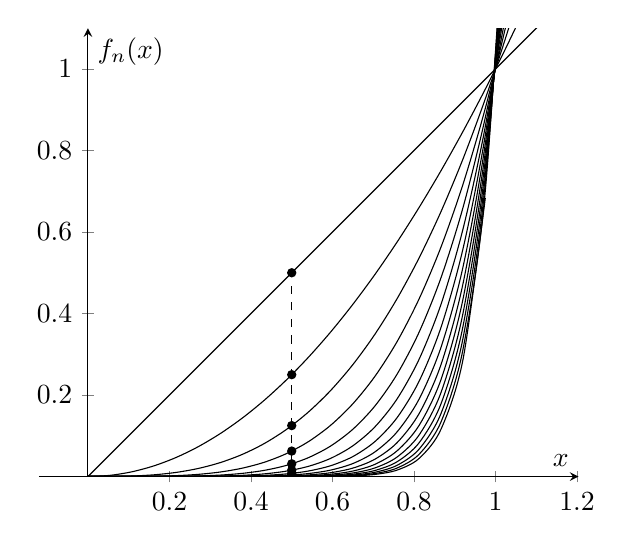
\begin{tikzpicture}
					\pgfmathsetmacro{\xzero}{.5}
					\begin{axis} [
						xlabel={$x$},ylabel={$f_n(x)$},
						axis lines=middle,
						axis equal,
						ymax = 1.1,
						legend pos = outer north east
					]
						\pgfplotsinvokeforeach{1,2,...,15} {
							% Restricting y fixes spurious lines being generated by Adobe Acrobat when printing the graph
							% Also, y domain is a bit bigger than the displayed graph since otherwise the functions wouldn't be properly plotted
							\addplot [smooth, domain=0:1.3, restrict y to domain=0:1.5] {pow(x, #1)};
							% This time around nodes are used instead of \addplot with the * mark
							% in order to control dots size, since bigger dots clutter the image
							\node[circle, fill=black, inner sep=1.2pt] at (\xzero, {pow(\xzero, #1)}) {};
						}

						\draw[dashed] (\xzero, 0) -- (\xzero, \xzero);
					\end{axis}
				\end{tikzpicture}
			}
			\caption{$x_0 = \frac{1}{2}$}
			\label{fig:conv_punt_grap_05}
		\end{subfigure}
		\begin{subfigure}{.33\textwidth}
			\centering
			\resizebox{\linewidth}{!}{
				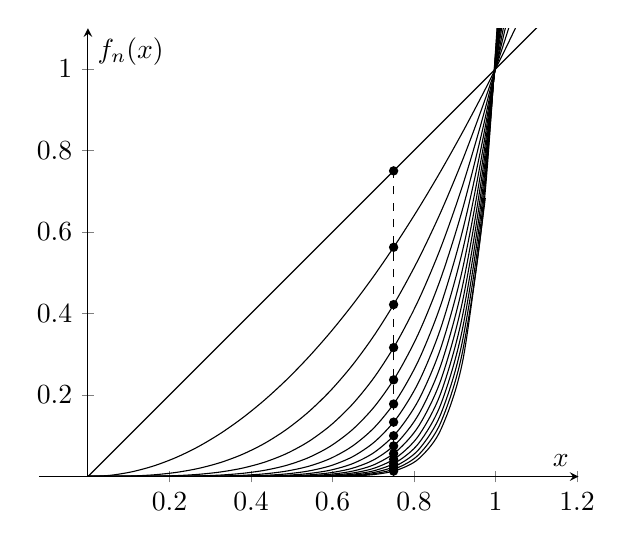
\begin{tikzpicture}
					\pgfmathsetmacro{\xzero}{.75}
					\begin{axis} [
						xlabel={$x$},ylabel={$f_n(x)$},
						axis lines=middle,
						axis equal,
						ymax = 1.1,
						legend pos = outer north east
					]
						\pgfplotsinvokeforeach{1,2,...,15} {
							% Restricting y fixes spurious lines being generated by Adobe Acrobat when printing the graph
							% Also, y domain is a bit bigger than the displayed graph since otherwise the functions wouldn't be properly plotted
							\addplot [smooth, domain=0:1.3, restrict y to domain=0:1.5] {pow(x, #1)};
							% This time around nodes are used instead of \addplot with the * mark
							% in order to control dots size, since bigger dots clutter the image
							\node[circle, fill=black, inner sep=1.2pt] at (\xzero, {pow(\xzero, #1)}) {};
						}

						\draw[dashed] (\xzero, 0) -- (\xzero, \xzero);
					\end{axis}
				\end{tikzpicture}
			}
			\caption{$x_0 = \frac{3}{4}$}
			\label{fig:conv_punt_grap_075}
		\end{subfigure}
		\begin{subfigure}{.33\textwidth}
			\centering
			\resizebox{\linewidth}{!}{
				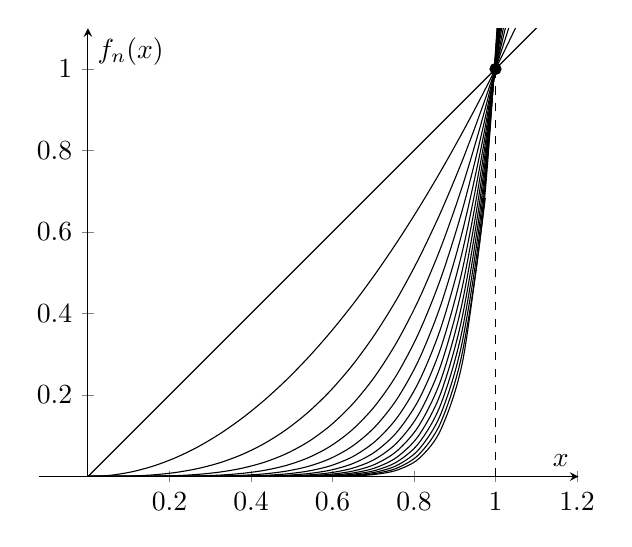
\begin{tikzpicture}
					\pgfmathsetmacro{\xzero}{1}
					\begin{axis} [
						xlabel={$x$},ylabel={$f_n(x)$},
						axis lines=middle,
						axis equal,
						ymax = 1.1,
						legend pos = outer north east
					]
						\pgfplotsinvokeforeach{1,2,...,15} {
							% Restricting y fixes spurious lines being generated by Adobe Acrobat when printing the graph
							% Also, y domain is a bit bigger than the displayed graph since otherwise the functions wouldn't be properly plotted
							\addplot [smooth, domain=0:1.3, restrict y to domain=0:1.5] {pow(x, #1)};
						}

						\addplot [color=black, only marks, mark=*] coordinates {(\xzero, \xzero)};
						\draw[dashed] (\xzero, 0) -- (\xzero, \xzero);
					\end{axis}
				\end{tikzpicture}
			}
			\caption{$x_0 = 1$}
			\label{fig:conv_punt_grap_1}
		\end{subfigure}
		\caption{Si vede che, al crescere di $n$, le $f(x_0)$ convergono a $0$ (in \ref{fig:conv_punt_grap_05} e \ref{fig:conv_punt_grap_075}) o $1$ (in \ref{fig:conv_punt_grap_1})}
	\end{figure}
\end{observation}

\begin{example}
	\label{ex:1_over_n_sin_x_punt_conv}
	La successione di Funzioni con $x \in A \equiv \R$
	\[f_n(x)=\frac{1}{n} \sin(x)\]
	è puntualmente convergente a $0$ su tutto il dominio delle $f_n$, cioè $f_n \pconvarrow 0$ su $B = A = \R$, infatti:
	\[
		\lim\limits_{n \to \infty} f_n(x) = \lim\limits_{n \to \infty} \frac{1}{n} \sin(x) = 0 \quad \forall x \in A
	\]
\end{example}
\begin{example}
	La successione
	\[f_n(x)=e^{nx}\]
	\begin{center}
		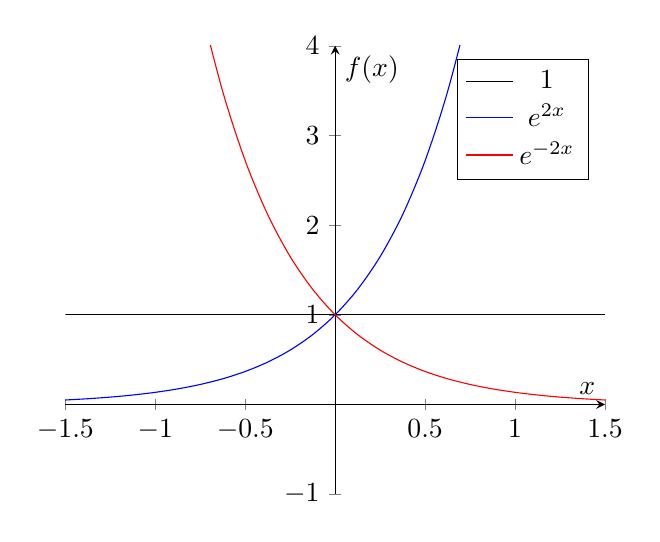
\begin{tikzpicture}
			\begin{axis}[
					xlabel={$x$},ylabel={$f(x)$},
					axis lines=middle,
					domain=-1.5:1.5,
					ymin=-1,ymax=4,
					legend pos = north east
				]
				\addplot[smooth] {1};
				\addlegendentry{$1$}
				\addplot[blue, smooth] {e^(2*x)};
				\addlegendentry{$e^{2x}$}
				\addplot[red, smooth] {e^(-2*x)};
				\addlegendentry{$e^{-2x}$}
			\end{axis}
		\end{tikzpicture}
	\end{center}
	Ha questo comportamento
	\[
		\lim\limits_{n \to \infty} e^{nx} =
		\begin{cases}
			\begin{array}{ll}
				0 & x<0\\
				1 & x=0\\
				\infty & x>0
			\end{array}
		\end{cases}
	\]
	Dunque
	\[f_n \pconvarrow f\quad \text{ su } B = \intervalopcl{-\infty}{0}\]
\end{example}

\begin{proposition}
	\label{prop:conv_punt_lim_succ}
	Siano $B \subseteq A \subseteq \R$, $\brackets{f_n:\; n \in \N}$ una \textbf{Successione di Funzioni} con $f_n:\; A \to \R$ e $f:\; B \to \R$. Allora
	\[
		f_n \pconvarrow f \text{ su } B \text{ per } n \to +\infty
		\quad \iff \quad
		\begin{cases}
			\forall \varepsilon > 0 \quad \forall x \in B\\
			\exists \nu \in \N:\; \forall n > \nu \quad \abs{f_n(x) - f(x)} \leq \varepsilon
		\end{cases}
	\]
	\begin{proof}
		Da \fullref{def:succ_punt_conv} si sa che
		\[f(x) = \lim\limits_{n \to +\infty} f_n(x) \qquad \forall x \in B\]
		Dunque, applicando la \fullref{def:lim_succ}
		\[
			\forall \varepsilon > 0 \quad \exists\nu\in\N:\; \forall n > \nu \quad d \bigl( f_n(x), f(x) \bigr) < \varepsilon  \qquad \forall x \in B
		\]
		Essendo in $f_n$ e $f$ a valori in $\R$, la $d$ è Metrica Euclidea, dunque
		\[
			\forall \varepsilon > 0 \quad \forall x \in B \quad \exists\nu\in\N:\; \forall n > \nu \quad \abs{f_n(x) - f(x)} < \varepsilon
		\]
		\vspace*{-\baselineskip}
		\begin{note}
			È possibile spostare $\forall x \in B$ "a sinistra dei $:$", in quanto, per definizione di $f$ dalla \fullref{def:succ_punt_conv}, $\forall x \in B \quad f(x) = \lim$, quindi la relazione è sempre valida, a prescindere dalla scelta di $x$.
		\end{note}
	\end{proof}
\end{proposition}
\begin{proposition}
	Siano $B \subseteq A \subseteq \R$, $\brackets{f_n:\; n \in \N}$ una \textbf{Successione di Funzioni} con $f_n:\; A \to \R$ e $F:\; B \to \R$. Allora
	\[
		\sum\limits_{n = 0}^{+\infty} f_n \pconvarrow F \text{ su } B
		\quad \iff \quad
		\begin{cases}
			\forall \varepsilon > 0 \quad \forall x \in B\\
			\exists \nu \in \N:\; \forall n > \nu \quad \abs{\sum\limits_{n = 0}^{k} f_n(x) - F(x)} \leq \varepsilon
		\end{cases}
	\]
	\begin{proof}
		Analoga alla \fullref{prop:conv_punt_lim_succ} ricordando la definizione di $F$ in \fullref{def:serie}.
	\end{proof}
\end{proposition}

\begin{proposition}[Metaproposizione sulle Proprietà delle Successioni]
	Sia $f_n:\; A \to \R$, $B \subseteq A \subseteq \R$, $f:\; B \to \R$\\
	Se $f_n \pconvarrow f$ su $B$ e se $f_n$ ha la proprietà $P$, allora la funzione limite puntuale $f$ ha a sua volta la proprietà $P$.
	\begin{note}
		La continuità (e quindi anche la derivabilità) non è una proprietà che passa alla funzione limite, come visto in \fullref{ex:conv_succ_xn}, dove la $f$ ha un punto di discontinuità in $x = 1$.
	\end{note}
	\begin{proof}
		Verrà svolta per le singole proprietà.
	\end{proof}
\end{proposition}
\begin{exercise}
	\label{ex:dim_prop_lim_conv_punt}
	Enunciare rigorosamente e dimostrare:
	\begin{enumerate}
		\item Il limite puntuale della somma (prodotto, combinazione lineare) di due successioni di funzioni è la somma (prodotto, combinazione lineare) delle funzioni limiti puntuali
		\item \label{itm:prop_lim_punt_non_neg} Il limite puntuale di una successione di funzioni non negative è una funzione non negativa
		\item \label{itm:prop_lim_punt_monotonia} Il limite puntuale di una successione di funzioni debolmente/strettamente crescenti/decrescenti è una funzione debolmente crescente/decrescente
		\item Il Criterio di Cauchy (da \fullref{def:succ_cau}) per la convergenza puntuale di serie e successioni
		\item Se la serie $\sum\limits_{n = 0}^{+\infty} f_n(x)$ converge puntualmente in un insieme $B$, allora $f_n \pconvarrow 0$ su $B$
	\end{enumerate}
	\begin{solution}~
		\renewcommand\qedsymbol{$\square$} % To restore the default empty square for the proof environments below
		\begin{enumerate}
			\item[\ref{itm:prop_lim_punt_non_neg}.]
				Sia $f_n:\; A \to \R$, $B \subseteq A \subseteq \R$ e $f:\; B \to A$\\
				Se $f_n \pconvarrow f$ su $B$ e se $f_n$ è non negativa su $B$, cioè $f_n \geq 0$, allora il limite puntuale $f$ è non negativo, $f \geq 0$, su $B$.
				\begin{proof}
					Da \fullref{def:succ_punt_conv}, si sa che
					\[f(x) = \lim\limits_{n \to \infty} f_n(x) \quad \forall x \in B\]
					Ma $f_n$ è, per ipotesi, una successione di valori non negativi, quindi il limite esiste ed è non negativo.

					La dimostrazione è analoga per funzioni non positive.
				\end{proof}
			\item[\ref{itm:prop_lim_punt_monotonia}.]
				Sia $f_n:\; A \to \R$, $B \subseteq A \subseteq \R$ e $f:\; B \to A$\\
				Se $f_n \pconvarrow f$ su $B$ e se $f_n$ è debolmente crescente su $B$, allora il limite puntuale $f$ è debolmente crescente su $B$.
				\begin{proof}
					Il fatto che $f_n$ sia debolmente crescente su $B$ implica che
					\[\forall x_1, x_2 \in B \quad x_1 \leq x_2 \implies f_n(x_1) \leq f_n(x_2)\]
					Con $n \to \infty$, essendo nell'insieme $B$, si ha che $f(x_1) \leq f(x_2)$ per definizione di $f$ da \fullref{def:succ_punt_conv}.

					La dimostrazione è analoga per funzioni debolmente decrescenti e strettamente/debolmente crescenti.
					\let\qed\relax % In order to avoid having two squares, hide the innermost one
				\end{proof}
			% TODO remaining points
			\vspace*{-2\baselineskip} % To remove the whitespace due to enumerate environment
		\end{enumerate}
	\end{solution}
\end{exercise}
\begin{observation}
	In riferimento al punto \ref{itm:prop_lim_punt_non_neg} dell'\fullref{ex:dim_prop_lim_conv_punt}, è necessario sottolineare come non sia invece possibie avere certezze sulla \textbf{stretta} positività/negatività del limite puntuale di una successione di funzioni strettamente positive/negative.\\
	Ad esempio, $-\frac{e^x}{n}$ con $x \in \intervalclop{0}{1}$ è strettamente negativa, ma il limite puntuale è costante $0$.
\end{observation}
\begin{observation}
	In riferimento al punto \ref{itm:prop_lim_punt_monotonia} dell'\fullref{ex:dim_prop_lim_conv_punt}, è necessario sottolineare come non sia invece possibie avere certezze sulla \textbf{stretta} crescenza/decrescenza del limite puntuale.\\
	Come esempio, vedasi \fullref{ex:conv_succ_xn} in cui si studia la successione strettamente crescente $x^n$, il cui limite puntuale è però costante (dunque non \textbf{strettamente} crescente) in $B = \intervalclop{0}{1}$.
\end{observation}
\begin{exercise}
	Verificare che il limite puntuale di funzoni \textbf{Continue} e \textbf{Derivabili}, quando esiste, può essere una funzione \textbf{Continua} e \textbf{non Derivabile}.\\
	Considerare ad esempio $f_n:\; \R \to \R$ data da $f_n(x) = \sqrt{x^2 + \frac{1}{n}}$ visibile in \cref{fig:fn_sqrt_x2_1_over_n}.
	% TODO solution
\end{exercise}
\begin{exercise}
	Verificare che il limite puntuale di funzoni \textbf{Continue} e \textbf{Derivabili}, quando esiste, può essere una funzione \textbf{non Continua}.\\
	Considerare ad esempio $f_n:\; \R \to \R$ data da $f_n(x) = \arctan(nx)$ visibile in \cref{fig:fn_sqrt_x2_1_over_n}.
	% TODO solution
\end{exercise}
\begin{exercise}
	Determinare, se possibile, sotto quali ipotesi sulla funzione $f:\; \R \to \R$ le seguenti successioni di funzioni risultano Puntualmente Convergenti:
	\begin{alignat*}{2}
		f_n(x) &= f(x) + n \hspace*{.35\linewidth} & f_n(x) &= f(x + n)\\
		f_n(x) &= f(x) + \frac{1}{n} & f_n(x) &= f(x + \frac{1}{n})\\
		f_n(x) &= nf(x) & f_n(x) &= \frac{f(x)}{n}\\
		f_n(x) &= f(nx) & f_n(x) &= f(\frac{x}{n})
	\end{alignat*}
\end{exercise}

\cbstart
\begingroup
% This group is used to alter equation numbering, since there are equations outside environments
\renewcommand\theequation{\arabic{section}.\arabic{equation}}
\setcounter{equation}{0} % Reset counter to fix numbering for equation outside theorem envs
\subsection{L'Insufficienza della Convergenza Puntuale}\label{sect:insuff_conv_punt}
La Convergenza Puntuale si può rivelare insufficiente per diverse ragioni, tra cui:
\begin{itemize}
	\item
		Può spesso esser comodo utilizzare una successione $f_n$ convergente puntualmente a $f$ nel caso in cui $f$ non sia ottenibile in modo esplicito (ad esempio nella soluzione di un'equazione differenziale). Però, come visto in \fullref{ex:conv_succ_xn}, la convergenza puntuale non trasferisce necessariamente proprietà come Continuità, Limitatezza o Derivabilità alla funzione limite puntuale.
		La successione $f_n = x^n$ di \fullref{ex:conv_succ_xn}, ad esempio, è formata da funzioni $\in \cntclass{\infty}(\intervalclose{0}{1}; \R)$, però la funzione limite puntuale
		\[
			f =
			\begin{cases}
				\begin{array}{ll}
					0 & \text{se } x \in \intervalopen{-1}{1}\\
					1 & \text{se } x = 1
				\end{array}
			\end{cases}
		\]
		non è né continua né, dunque, derivabile nello stesso intervallo.
		\begin{figure}[H]
			\begin{subfigure}{.49\textwidth}
				\centering
				\resizebox{\linewidth}{!}{
					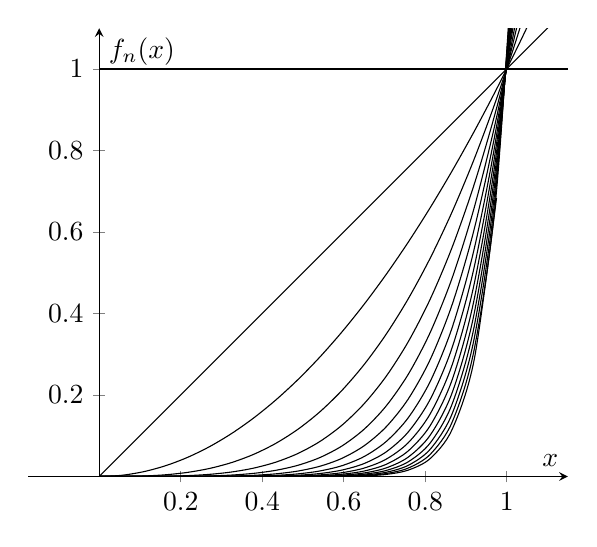
\begin{tikzpicture}
						\begin{axis} [
							xlabel={$x$},ylabel={$f_n(x)$},
							axis lines=middle,
							axis equal,
							% xmax is used only to force same width to both graphs, thus having same height when resized
							ymax = 1.1, xmax = 1.15,
							legend pos = outer north east
						]
							\pgfplotsinvokeforeach{0,1,...,15} {
								% Restricting y fixes spurious lines being generated by Adobe Acrobat when printing the graph
								% Also, y domain is a bit bigger than the displayed graph since otherwise the functions wouldn't be properly plotted
								\addplot [smooth, domain=0:1.3, restrict y to domain=0:1.5] {pow(x, #1)};
							}
						\end{axis}
					\end{tikzpicture}
				}
				\caption{$f_n(x) = x^n \quad 0 \leq n \leq 15$}
			\end{subfigure}
			\begin{subfigure}{.49\textwidth}
				\centering
				\resizebox{\linewidth}{!}{
					\begin{tikzpicture}
						\begin{axis} [
							xlabel={$x$},ylabel={$f(x)$},
							axis lines=middle,
							axis equal,
							% xmax is used only to force same width to both graphs, thus having same height when resized
							ymax = 1.1, xmax = 1.15,
							legend pos = outer north east
						]
							\addplot [smooth, line width=2pt, domain=0:1] {0};
							\addplot [color=black, fill=white, only marks, mark=*] coordinates {(1,0)};
							\addplot [color=black, only marks, mark=*] coordinates {(1,1)};
						\end{axis}
					\end{tikzpicture}
				}
				\caption{$f(x) \quad x \in \intervalclose{0}{1}$}
			\end{subfigure}
			\caption{$f_n(x) \in \cntclass{\infty}(\intervalclose{0}{1}; \R)$, mentre la funzione limite puntuale $f$ è discontinua.}
			\label{fig:cont_fn_non_passa_a_f}
		\end{figure}
	\item
		Supponendo di voler calcolare l'integrale
		\begin{equation}
			\label{eq:insuf_conv_punt_int_f}
			\int_a^b f(x) \integrald{x}
		\end{equation}
		Ma con $f$ non integrabile (o magari anche solo $f$ non integrabile in modo elementare). Si cercherebbe dunque di approssimarlo con una successione di integrali tipo
		\begin{equation}
			\label{eq:insuf_conv_punt_int_fn}
			\int_a^b f_n(x) \integrald{x}
		\end{equation}
		Potrebbe venire naturale di prendere una successione $f_n$ Puntualmente Convergente a $f$ e quindi considerare gli integrali delle $f_n$ della \cref{eq:insuf_conv_punt_int_fn} come approssimazioni dell'integrale \cref{eq:insuf_conv_punt_int_f}. Questo ragionamento è però valido solo nel caso in cui valga
		\begin{equation}
			\label{eq:conv_punt_pass_lim_integrale}
			\lim\limits_{n \to +\infty} \int_a^b f_n(x) \integrald{x} = \int_a^b \lim\limits_{n \to +\infty} f_n(x) \integrald{x} = \int_a^b f(x) \integrald{x}
		\end{equation}
		Cioè eseguendo il \textit{passaggio al limite sotto il segno di integrale}, operazione di cui si è già parlato nell'introduzione al \fullref{chap:int_doppi} specificando che, con gli integrali di Riemann, non è affatto scontato sia possibile.\\
		Nel caso della convergenza puntuale non son garantite le iptesi necessarie, dunque non è possibile passare al limite sotto l'integrale, come si vede nel successivo \fullref{ex:conv_punt_no_pass_lim_integrale}.
\end{itemize}
La Convergenza Puntuale presenta le problematiche evidenziate in quanto non si basa su alcun tipo di concetto di \textbf{distanza tra funzioni}. Infatti, ricordando \fullref{def:succ_punt_conv}, avere convergenza puntuale $f_n \pconvarrow f$ su un certo insieme $A$ significa che, fissato un qualsiasi $x_0 \in A$, si ha
\[\lim\limits_{n \to +\infty} d \bigl( f_n(x_0), f(x_0) \bigr) = 0\]
Con $d$ Metrica Euclidea, distanza tra i valori di $f_n$ ed $f$ nel punto $x_0$ precedentemente fissato. In pratica, i valori di $f_n$ e $f$ vengono considerati \textbf{punto per punto} separatamente e la convergenza puntuale non è influenzata da tutti gli altri valori che le funzioni possono assumere in un intorno di $x_0$.
\begin{example}
	\label{ex:conv_punt_no_pass_lim_integrale}
	La successione
	\[
		\funcdef{f_n}{\intervalclose{0}{1}}{\R}{x}{
			\begin{cases}
				\begin{array}{ll}
					0 & \text{se } x \in \brackets{0} \cup \intervalopcl{\frac{1}{n}}{1}\\
					-n^2x + n & \text{se } x \in \intervalopcl{0}{\frac{1}{n}}
				\end{array}
			\end{cases}
		}
	\]
	converge puntualmente alla funzione $f(x) = 0$ su $\intervalclose{0}{1}$. Infatti, essendo $\frac{1}{n} \to 0$ per $n \to +\infty$, un qualsiasi $x \in \intervalclose{0}{1}$ cadrà nell'intervallo $\intervalopcl{\frac{1}{n}}{1}$ in cui $f_n$ è definita essere $0$. Quindi $\lim\limits_{n \to +\infty} f_n(x) = 0$.
	\begin{center}
		\begin{tikzpicture}
			\begin{axis} [
				clip mode = individual,
				xlabel={$x$},ylabel={$f_n(x)$},
				axis lines=middle,
				xmax=1.2, ymax=5.5,
				xtick = {1/2, 1},
				xticklabels = {$\frac{1}{n}$, $1$},
				ytick = {2},
				yticklabels = {$n$}
			]
				\addplot [color=black, only marks, mark=*] coordinates {(0,0)};
				\pgfplotsinvokeforeach{2, 3, 5} {
					\addplot [thick, domain=0:(1/#1)] {-pow(#1, 2)*x + #1};
					\addplot [color=black, fill=white, only marks, mark=*] coordinates {(0,#1)};
				}
				\addplot [line width=2pt, domain=(1/5):1] {0}; % We need only a single line on x axis, the one starting at the smallest 1/n
			\end{axis}
		\end{tikzpicture}
	\end{center}
	Gli integrali delle $f_n$ sono:
	\begin{align*}
		&\int_0^1 f_n(x) \integrald{x} =\\
		&= \int_0^{\frac{1}{n}} \left( -n^2x + n \right)\integrald{x} + \int_{\frac{1}{n}}^1 0 \integrald{x}\\
		&= \left[ -\frac{n^2}{2}x^2 + nx \right]_0^{\frac{1}{n}}\\
		&= -\frac{n^2}{2}\frac{1}{n^2} + n \frac{1}{n}\\
		&= \frac{1}{2}
	\end{align*}
	L'integrale della funzione limite puntuale $f$ sarebbe, ovviamente, $0$, essendo stato dimostrato prima che $f_n \pconvarrow 0$, dunque l'uguaglianza di \cref{eq:conv_punt_pass_lim_integrale} non vale.
\end{example}

\subsection{Distanze tra Funzioni}\label{sect:dist_funz}
La nozione di distanza si basa, generalmente, su una preesistente nozione di "grandezza": stabilito il modo per valutare la grandezza di un ente, è ragionevole ritenere che due oggetti siano tanto più vicini quanto più è "piccola" la differenza tra essi. Cioè la distanza può essere vista come la "grandezza" della differenza (ovviamente, quando è ammessa la differenza tra gli oggetti). Si è vista l'applicazione di questo criterio in molti esempi di \fullref{ex:metriche}.

Dovendo valutare la distanza tra funzioni, è dunque necessario prima stabilire come valutare la "grandezza" delle funzioni stesse.

Quale delle seguenti funzioni ha senso definire "più grande"?
\begin{figure}[H]
	\begin{subfigure}{.49\textwidth}
		\centering
		\resizebox{\linewidth}{!}{
			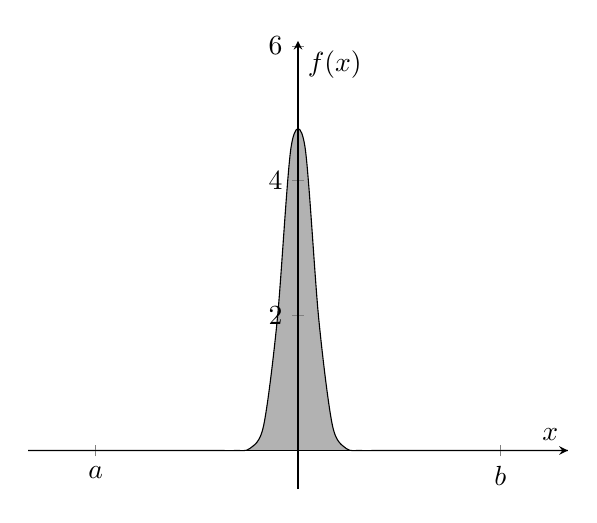
\begin{tikzpicture}
				\begin{axis} [
					xlabel={$x$},ylabel={$f(x)$},
					axis lines=center,
					axis on top = true,
					axis equal,
					xmin = -4, xmax = 4,
					ymin = -.5, ymax = 6,
					xtick = {-3, 3},
					xticklabels = {$a$, $b$}
				]
					\addplot [name path=f, smooth, domain=-5:5, samples=50] {exp(-10*x^2)*5};
					\path[name path=axis] (\pgfkeysvalueof{/pgfplots/xmin},0) -- (\pgfkeysvalueof{/pgfplots/xmax},0);
					\addplot[black!30] fill between[of=f and axis, soft clip={domain=-3:3}];
				\end{axis}
			\end{tikzpicture}
		}
		\caption{Curva gaussiana}
		\label{pic:grand_funz_gauss}
	\end{subfigure}
	\begin{subfigure}{.49\textwidth}
		\centering
		\resizebox{\linewidth}{!}{
			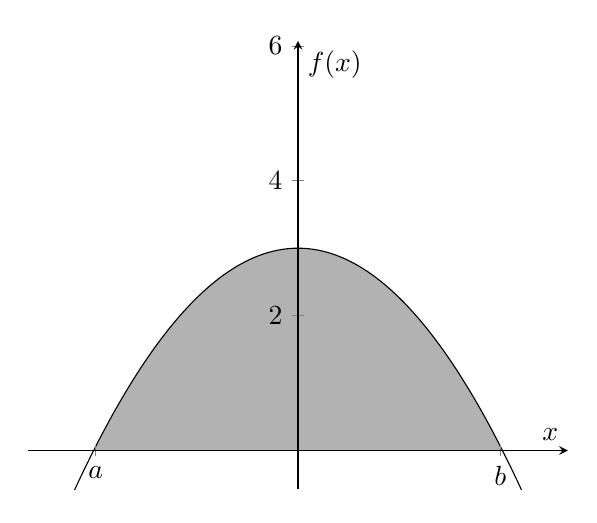
\begin{tikzpicture}
				\begin{axis} [
					xlabel = $x$, ylabel = {$f(x)$},
					axis lines = center,
					axis on top = true,
					axis equal,
					xmin = -4, xmax = 4,
					ymin = -.5, ymax = 6,
					xtick = {-3, 3},
					xticklabels = {$a$, $b$}
				]
					\addplot [name path=f, smooth, domain=-5:5, samples=50] {-(4/7*x)^2+3};
					\path[name path=axis] (\pgfkeysvalueof{/pgfplots/xmin},0) -- (\pgfkeysvalueof{/pgfplots/xmax},0);
					\addplot[black!30] fill between[of=f and axis, soft clip={domain=-3:3}];
				\end{axis}
			\end{tikzpicture}
		}
		\caption{Parabola rovesciata}
		\label{pic:grand_funz_parab}
	\end{subfigure}
	\caption{Diversi parametri per valutare la "grandezza" di una funzione}
\end{figure}

Ovviamente dipende dall'aspetto che si intende considerare. La \ref{pic:grand_funz_gauss} potrebbe essere "più grande" perché ha massimo maggiore rispetto a \ref{pic:grand_funz_parab}, che però d'altro canto ha una maggiore area sottesa.

Questi erano solo due esempi di "grandezza" di una funzione, definiti con le seguenti metriche
\[
	\norm{f}_{\cntclass{0}} = \sup\limits_{x \in \intervalclose{a}{b}} \abs{f(x)}
	\qquad\qquad\qquad\qquad\qquad
	\norm{f}_1 = \int_a^b \abs{f(x)} \integrald{x}
\]
Quella di sinistra è la \textbf{Norma Infinito} o \textbf{Norma del} $\boldsymbol{\sup}$, mentre a destra \textbf{Norma Indice} $\boldsymbol{1}$. In aggiunta, si definisce anche la \textbf{Norma Indice} $\boldsymbol{2}$, che sarà usata in \fullref{sect:conv_quadr}:
\[\norm{f}_2 = \sqrt{ \int_a^b \left[f(x)\right]^2 \integrald{x} }\]

Le distanze indotte dalle seguenti norme saranno dunque
\[
	d_{\cntclass{0}} (f, g) = \norm{f - g}_{\cntclass{0}}
	\qquad\qquad\qquad
	d_1 = \norm{f - g}_1
	\qquad\qquad\qquad
	d_2 = \norm{f - g}_2
\]
E si parla di \textbf{Distanza Infinito} (o \textbf{Distanza del} $\boldsymbol{\sup}$), \textbf{Distanza Indice} $\boldsymbol{1}$ e \textbf{Distanza Indice} $\boldsymbol{2}$.

\begin{figure}[H]
	\begin{subfigure}{.49\textwidth}
		\centering
		\resizebox{\linewidth}{!}{
			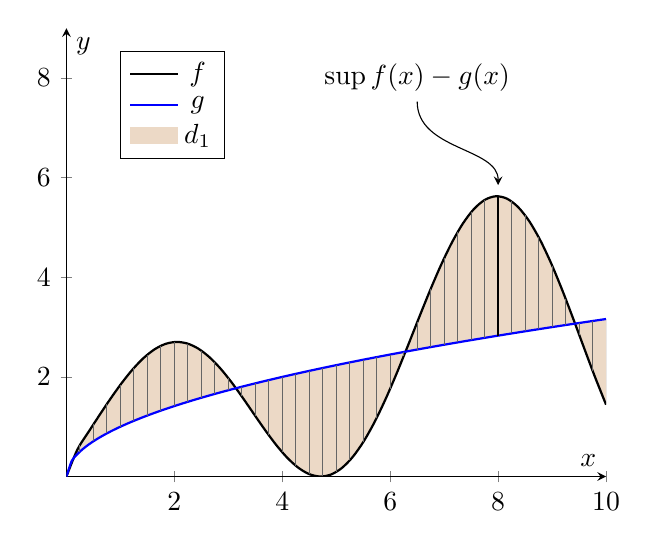
\begin{tikzpicture}[
				declare function = {
					f(\x) = sqrt(\x)*(sin(deg(\x))+1);
					g(\x) = sqrt(\x);
				},
				> = stealth
			]
			\begin{axis} [
				xlabel={$x$},ylabel={$y$},
				axis lines=middle,
				ymax=9,
				legend style = {at={(.1,.95)}, anchor = north west}
			]
				\addplot [thick, name path=f, smooth, domain=0:10, samples=50] {f(x)};
				\addlegendentry{$f$};
				\addplot [color=blue, thick, name path=g, smooth, domain=0:10, samples=100] {g(x)};
				\addlegendentry{$g$};
				\pgfplotsinvokeforeach{.25,.5,...,10} {
					\draw[thin, black!60] (#1, {f(#1)}) -- (#1, {g(#1)});
				}
				% Mark thicker the sup
				\draw[thick] (8, {g(8)}) -- (8,{f(8)});
				\node (text_sup_dist) [align=center] at (6.5,8) {$\sup \abs{f(x) - g(x)}$};
				\draw[thin, ->, shorten >=4pt] (text_sup_dist.south) to [out=-90, in=90](8,{f(8)});

				\addplot[brown!30] fill between[of=f and g];
				\addlegendentry{$d_1$};
			\end{axis}
		\end{tikzpicture}
		}
		\caption{Significato grafico di\\Distanza Infinito e Distanza Indice $1$}
	\end{subfigure}
	\begin{subfigure}{.49\textwidth}
		\centering
		\resizebox{\linewidth}{!}{
			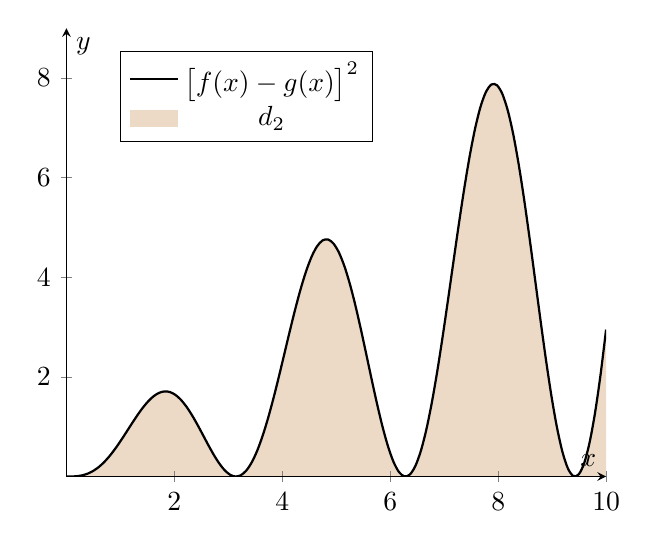
\begin{tikzpicture}[
				declare function = {
					f(\x) = sqrt(\x)*(sin(deg(\x))+1);
					g(\x) = sqrt(\x);
				},
				> = stealth
			]
				\begin{axis} [
					xlabel={$x$},ylabel={$y$},
					axis lines=middle,
					axis on top = true,
					ymax=9,
					legend style = {at={(.1,.95)}, anchor = north west}
				]
					\addplot [thick, name path=f, smooth, domain=0:10, samples=100] {(f(x)-g(x))^2};
					\addlegendentry{$\bigl[ f(x) - g(x) \bigr]^2$};
					\path[name path=axis] (\pgfkeysvalueof{/pgfplots/xmin},0) -- (\pgfkeysvalueof{/pgfplots/xmax},0);
					\addplot[brown!30] fill between[of=f and axis];
					\addlegendentry{$d_2$};
				\end{axis}
			\end{tikzpicture}
		}
		\caption{Significato grafico (a meno della radice) di\\Distanza Indice $2$}
	\end{subfigure}
\end{figure}
\cbend
\endgroup

\subsection{Convergenza Uniforme}\label{sect:conv_unif}
Si chiama convergenza uniforme la convergenza di una Successione rispetto alla distanza $d_{\cntclass{0}}$.

\begin{definition}[Successione Uniformemente Convergente]
	\label{def:succ_unif_conv}
	Siano $B \subseteq A \subseteq \R$, $\brackets{f_n:\; n \in \N}$ una \textbf{Successione di Funzioni} e $f_n:\; A \to \R$.\\
	La Successione $f_n$ è \textbf{Uniformemente Convergente} su $B$ se esiste la \textbf{Funzione Limite Uniforme} $f:\; B \to \R$ tale che:
	\[\lim\limits_{n \to +\infty} \sup\limits_{B} \abs{f_n(x) - f(x)} = 0\]
	\begin{note}
		Nella \fullref{def:succ_punt_conv} la $f$ associava ogni punto al valore a cui convergeva la successione in quel punto.\\
		In questo caso invece la $f$ è una funzione \textit{tale per cui} la distanza massima (per via del $\sup$ di $d_{\cntclass{0}}$) tra $f_n$ e $f$ è $0$. Questo vuol dire che la funzione "coincide con la $f_n$ su tutto $B$", in quel senso \textit{Uniformemente}. Vedasi \fullref{obs:diff_conv_unif_e_conv_punt}.
	\end{note}
	La convergenza uniforme su $B$ della successione $f_n$ verso $f$ è indicata con
	\[f_n \uconvarrow f \text{ su } B\]
\end{definition}
\begin{definition}[Serie Uniformemente Convergente]
	Siano $B \subseteq A \subseteq \R$, $\brackets{f_n:\; n \in \N}$ una \textbf{Successione di Funzioni} e $f_n:\; A \to \R$.\\
	La \textbf{Serie} $s = \sum\limits_{n = 0}^{+\infty} f_n(x)$ associata alla Successione $f_n$ è \textbf{Uniformemente Convergente} su $B$ se esiste la \textbf{Funzione Limite Uniforme} $F:\; B \to \R$ tale che:
	\[\lim\limits_{n \to +\infty} \sup\limits_{B} \abs{\sum\limits_{n = 0}^{+\infty} f_n(x) - F(x)} = 0\]
\end{definition}

\begin{example}~
	\begin{figure}[H]
		\centering
		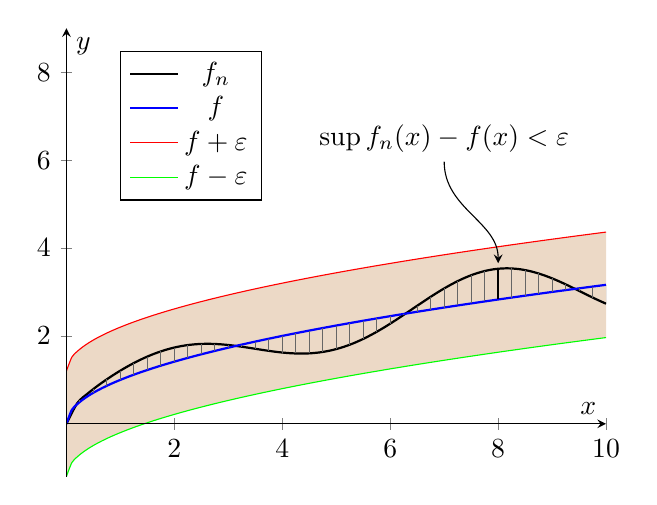
\begin{tikzpicture}[
			declare function = {
				f_n(\x) = sqrt(\x)*(1/4*(sin(deg(\x))+4));
				f(\x) = sqrt(\x);
			},
			> = stealth
		]
			\begin{axis} [
				xlabel={$x$},ylabel={$y$},
				axis lines=middle,
				axis on top = true,
				ymax=9,
				legend style = {at={(.1,.95)}, anchor = north west}
			]
				\addplot [thick, name path=f_n, smooth, domain=0:10, samples=50] {f_n(x)};
				\addlegendentry{$f_n$};
				\addplot [color=blue, thick, smooth, domain=0:10, samples=100] {f(x)};
				\addlegendentry{$f$};
				\addplot [color=red, name path=f_plus, smooth, domain=0:10, samples=100] {f(x) + 1.2};
				\addlegendentry{$f + \varepsilon$};
				\addplot [color=green, name path=f_minus, smooth, domain=0:10, samples=100] {f(x) - 1.2};
				\addlegendentry{$f - \varepsilon$};
				\pgfplotsinvokeforeach{.25,.5,...,10} {
					\draw[thin, black!60] (#1, {f_n(#1)}) -- (#1, {f(#1)});
				}
				% Mark thicker the sup
				\draw[thick] (8, {f(8)}) -- (8,{f_n(8)});
				\node (text_sup_dist) [align=center] at (7,6.5) {$\sup \abs{f_n(x) - f(x)} < \varepsilon$};
				\draw[thin, ->, shorten >=2pt] (text_sup_dist.south) to [out=-90, in=90](8,{f_n(8)});

				\addplot[brown!30, forget plot] fill between[of=f_plus and f_minus];
			\end{axis}
		\end{tikzpicture}
		\caption{Significato grafico della Convergenza Uniforme\\Come si vedrà in {\protect\fullref{prop:conv_unif_lim_succ}}}
	\end{figure}
\end{example}

\begin{observation}
	\label{obs:dist_conv_unif}
	La convergenza uniforme equivale alla convergenza rispetto alla distanza $d_{\cntclass{0}}(f,g)=\sup\limits_{x\in A}\abs{g(x)-f(x)}$ ogniqualvolta questa distanza sia definita. La definizione di $d_{\cntclass{0}}(f,g)$ come \textit{distanza} è dimostrata in \hyperref[ex:dim_dist_conv_unif]{\fullref*{ex:metriche}}\\
	% NOTE The \fullref command was not used on purpose to point this link straight to the right part of the aforementioned exercise
	La $d_{\cntclass{0}}(f,g)$ può anche essere definita attraverso la \textbf{norma} $\norm{k}_{\cntclass{0}}=\sup\limits_{x\in A}\abs{k}$ con $k = f-g$ in quanto, in $\R$ norma e valore assoluto coincidono.
\end{observation}
\begin{example}
	Come già visto in \fullref{ex:1_over_n_sin_x_punt_conv}, la Successione di Funzioni con $x \in A \equiv \R$
	\[f_n(x) = \frac{1}{n} \sin(x)\]
	è $f_n \pconvarrow 0$ su $A$. Questa stessa Successionione è anche Uniformemente Convergente su $A$, infatti:
	\[
		\lim\limits_{n \to +\infty} \sup\limits_{A} \abs{f_n(x) - 0} =
		\lim\limits_{n \to +\infty} \sup\limits_{A} \abs{\frac{1}{n} \sin(x)}
	\]
	Osservando che $\abs{a \cdot \sin(x)} \leq \abs{a}$, si può conclduere
	\[
		\lim\limits_{n \to +\infty} \sup\limits_{\R} \abs{\frac{1}{n} \sin(x)} \leq
		\lim\limits_{n \to +\infty} \frac{1}{n}=0
	\]
	Allora $f_n \uconvarrow f$ su $A$
\end{example}

\begin{exercise}
	\label{ex:dim_dist_inf}
	Sia $K \in \R$ un \textbf{Compatto}. Verificare che:
	\begin{enumerate}
		\item $\norm{\;\cdot\;}_{\cntclass{0}}$ è una norma su $\cntclass{0}(K; \R)$
		\item \label{itm:dim_dist_inf_dist} $d_{\cntclass{0}}$ è una distanza su $\cntclass{0}(K; \R)$
		\item La convergenza rispetto alla distanza $d_{\cntclass{0}}$ equivale alla convergenza uniforme su $K$
	\end{enumerate}
	\begin{solution}~
		\begin{enumerate}
			\item[\ref{itm:dim_dist_inf_dist}.] Dimostrata in \hyperref[ex:dim_dist_conv_unif]{\fullref*{ex:metriche}}
			% NOTE The \fullref command was not used on purpose to point this link straight to the right part of the aforementioned exercise
		\end{enumerate}
		% TODO remaining points proof
	\end{solution}
\end{exercise}
\begin{proposition}
	\label{prop:conv_unif_lim_succ}
	Siano $B \subseteq A \subseteq \R$, $\brackets{f_n:\; n \in \N}$ una \textbf{Successione di Funzioni} e $f_n:\; A \to \R$. Sia $f:\; B \to \R$ una funzione:
	\[
		f_n \uconvarrow f \text{ su } B \text{ per } n \to +\infty
		\quad \iff \quad
		\begin{cases}
			\forall \varepsilon > 0 \quad \exists \nu \in \N:\\
			\forall n > \nu \quad \forall x \in B \quad \abs{f_n(x) - f(x)} \leq \varepsilon
		\end{cases}
	\]
	\begin{solution}
		Da \fullref{def:succ_unif_conv} si sa che
		\[\lim\limits_{n \to +\infty} \sup\limits_{B} \abs{f_n(x) - f(x)} = 0\]
		Dunque, applicando la \fullref{def:lim_succ}
		\[
			\forall \varepsilon > 0 \quad \exists\nu\in\N:\; \forall n > \nu \quad d \bigl( \abs{f_n(x) - f(x)}, 0 \bigr) < \varepsilon  \qquad \forall x \in B
		\]
		Essendo in $f_n$ e $f$ a valori in $\R$, la $d$ è Metrica Euclidea, dunque
		\[
			\forall \varepsilon > 0 \quad \exists\nu\in\N:\; \forall n > \nu \quad \forall x \in B \quad \bigl| \abs{f_n(x) - f(x)} - 0 \bigr| < \varepsilon
		\]
		\begin{note}
			A differenza di quanto fatto in \fullref{prop:conv_punt_lim_succ}, non è possibile spostare $\forall x \in B$ "a sinistra dei $:$". La scelta di $x$ non è \textit{"a prescindere"}, ma subordinata alla scelta di $\varepsilon$ e $\nu$. Dato dunque un certo $\nu$, allora, per ogni $n$ e $x$, vale il limite. Vedasi \fullref{obs:diff_conv_unif_e_conv_punt}.
		\end{note}
	\end{solution}
\end{proposition}
\begin{proposition}
	Siano $B \subseteq A \subseteq \R$, $\brackets{f_n:\; n \in \N}$ una \textbf{Successione di Funzioni} con $f_n:\; A \to \R$ e $F:\; B \to \R$. Allora
	\[
		\sum\limits_{n = 0}^{+\infty} f_n \uconvarrow F \text{ su } B
		\quad \iff \quad
		\begin{cases}
			\forall \varepsilon > 0 \quad \exists \nu \in \N:\\
			\forall n > \nu \quad \forall x \in B \quad \abs{\sum\limits_{n = 0}^{k} f_n(x) - F(x)} \leq \varepsilon
		\end{cases}
	\]
	\begin{proof}
		Analoga alla \fullref{prop:conv_unif_lim_succ} ricordando la definizione di $F$ in \fullref{def:serie}.
	\end{proof}
\end{proposition}
\begin{observation}
	\label{obs:diff_conv_unif_e_conv_punt}
	La differenza tra \fullref{prop:conv_unif_lim_succ} e \fullref{prop:conv_punt_lim_succ} (e rispettive proposizioni sulle Serie) giustifica il fatto che la continuità non passi alla Funzione Limite Puntuale, come spiegato in \fullref{sect:insuff_conv_punt}.

	Infatti qui $\nu$ dipende solo dalla scelta di $\varepsilon$ e le $x$ "si guardano tutte insieme", nella Convergenza Puntuale invece $\nu$ dipendeva, oltre che dalla $\varepsilon$, anche dalla $x$. Questo portava ad osservare le $x$ una alla volta.
\end{observation}
\begin{corollary}[Relazione tra Convergenza Uniforme e Puntuale]
	\label{coro:if_unif_conv_then_punt_conv}
	Siano $B \subseteq A \subseteq \R$ e $\brackets{f_n:\; n \in \N}$ una \textbf{Successione di Funzioni} e $f_n:\; A \to \R$. Sia $f:\; B \to \R$ una funzione
	\[f_n \uconvarrow f \text{ su } B \quad \implies \quad  f_n \pconvarrow f \text{ su } B\]
	\vspace*{-\baselineskip}
	\begin{note}
		Questo significa che la Convergenza Uniforme ha tutte le proprietà della Convergenza Puntuale.
	\end{note}
	\begin{note}
		L'implicazione inversa non è possibile, come si vede in \fullref{ex:conv_punt_nimplies_conv_unif}.
	\end{note}
	\begin{proof}
		Da \fullref{prop:conv_unif_lim_succ}  si sa che valgono condizioni analoghe, ma più restrittive, rispetto a quelle di \fullref{prop:conv_punt_lim_succ} (vedere note alle due Proposizioni), dunque sicuramente è valida l'implicazione $\impliedby$ di \fullref{prop:conv_punt_lim_succ}.
	\end{proof}
\end{corollary}
\begin{example}[La Convergenza Puntuale non implica Convergenza Uniforme]
	\label{ex:conv_punt_nimplies_conv_unif}
	Sia $f_n:\; \R \to \R$ data da $f_n(x) = x^n$, allora:
	\[
		f_n \pconvarrow f \text{ su } \intervalopcl{-1}{1}
		\qquad \text{dove} \qquad
		f(x) = \begin{cases}
			\begin{array}{ll}
				0 & \text{per } x \in \intervalopen{-1}{1}\\
				1 & \text{per } x = 1
			\end{array}
		\end{cases}
	\]
	Ma su $\intervalopcl{-1}{1}$ non c'è convergenza uniforme e nemmeno su $\intervalopen{-1}{1}$.
\end{example}
\begin{exercise}
	È possibile costruire una successione di funzioni $f_n$ uniformemente convergenti ad una successione $f$ non limitata?
	\begin{solution}
		No, perché, come visto in \fullref{coro:if_unif_conv_then_punt_conv} $f_n \uconvarrow f \implies f_n \pconvarrow f$, ma per \fullref{def:succ_punt_conv} $\nexists$ successione puntualmente convergente a $f$ non limitata.
		% TODO controllare soluzione
	\end{solution}
\end{exercise}
\begin{exercise}
	Determinare, se possibile, sotto quali ipotesi sulla funzione $f:\; \R \to \R$ le seguenti successioni di funzioni sono Uniformemente Convergenti:
	\begin{alignat*}{2}
		f_n(x) &= f(x) + n \hspace*{.35\linewidth} & f_n(x) &= f(x + n)\\
		f_n(x) &= f(x) + \frac{1}{n} & f_n(x) &= f(x + \frac{1}{n})\\
		f_n(x) &= nf(x) & f_n(x) &= \frac{f(x)}{n}\\
		f_n(x) &= f(nx) & f_n(x) &= f(\frac{x}{n})
	\end{alignat*}
\end{exercise}
\begin{definition}[Successione di Funzioni di Cauchy per la Convergenza Uniforme]
	\label{def:succ_funz_cau}
	Siano $B \subseteq A \subseteq \R$, $\brackets{f_n:\; n \in \N}$ una \textbf{Successione di Funzioni} e $f_n:\; A \to \R$
	\begin{center}
		La Successione $\brackets{f_n:\; n \in \N}$ soddisfa alla \textbf{Condizione di Cauchy}\\
		per la \textbf{Convergenza Uniforme} su $B$\\
		$\bydef$\\
		$
			\forall \varepsilon > 0 \quad \exists \nu \in \N: \quad \forall n, m > \nu \quad \forall x \in B %
			\qquad \text{vale} \qquad \abs{f_n(x) - f(x)} < \varepsilon
		$
	\end{center}
\end{definition}
\begin{proposition}
	\label{prop:in_compat_succ_funz_cau_corrisp_a_succ_cau}
	Nel caso in cui $B$ sia \textbf{Compatto}, la \fullref{def:succ_funz_cau} coincide alla \fullref{def:succ_cau}.
	\begin{proof}
		Dalla \fullref{def:compatto}, si sa che ogni successione ammette una sottosuccessione avente limite in $B$, dunque si arriva ad avere la distanza $d \left( \lim\limits_{n \to +\infty}f_n(x), f(x) \right)$ tra due elementi di $K$.
	\end{proof}
\end{proposition}
\begin{definition}[Serie di Funzioni di Cauchy per la Convergenza Uniforme]
	Siano $B \subseteq A \subseteq \R$, $\brackets{f_n:\; n \in \N}$ una \textbf{Successione di Funzioni} e $f_n:\; A \to \R$
	\begin{center}
		La Serie $\sum\limits_{n = 0}^{+\infty}$ associata alla Successione $f_n$ soddisfa alla \textbf{Condizione di Cauchy}\\
		per la \textbf{Convergenza Uniforme} di serie su $B$\\
		$\bydef$\\
		$
			\forall \varepsilon > 0 \quad \exists \nu \in \N:\; \forall n, m > \nu \quad \forall x \in B %
			\qquad \text{vale} \qquad \abs{ \sum\limits_{k = n}^{m} f_k(x) } < \varepsilon
		$
	\end{center}
\end{definition}

\begin{proposition}
	\label{prop:succ_funz_cau_allora_esiste_f_conv_unif}
	Siano $B \subseteq A \subseteq \R$, $\brackets{f_n:\; n \in \N}$ una \textbf{Successione di Funzioni} e $f_n:\; A \to \R$
	\[
		\left.
			\begin{array}{c}
				\text{La Successione } f_n \text{ soddisfa}\\
				\text{alla \textbf{Condizione di Cauchy}}\\
				\text{per la \textbf{Convergenza Uniforme} su } B
			\end{array}
		\right\}
		\implies
		\begin{cases}
			\begin{array}{c}
				\text{Esiste una funzione}\\
				f:\; B \to \R\\
				\text{tale che } f_n \uconvarrow f \text{ su } B
			\end{array}
		\end{cases}
	\]
	\begin{proof}
		Se la successione $\brackets{f_n:\; n \in \N}$ soddisfa la \fullref{def:succ_funz_cau} su $B$\\
		$\implies$ ogni successione $\brackets{f_n(x):\; n \in \N},\; \forall x \in B$, è di Cauchy in $\R$\\
		$\implies$ essendo $\R$ Completo, per \fullref{def:completo} ogni successione
		\[\brackets{f_n(x):\; n \in \N},\; \forall x \in B\]
		avrà limite in $\R$. Sia posta ora $f(x)$ la funzione che associa ad ogni $x$ il limite della $f_n(x)$.

		Si verifica che $f$ è la Funzione Limite Uniforme della successione $\brackets{f_n(x):\; n \in \N}$ su $B$. Infatti, posto $\varepsilon > 0$, sia $\nu \in \N$ tale che $\sup\limits_{B} \abs{f_h - f_k} < \varepsilon$ per ogni $h, k \in B$. Allora si ha:
		\begin{align*}
			&\sup\limits_{B} \abs{f_h - f_k} < \varepsilon \quad \forall h, k > \nu
			\shortintertext{Essendo $\sup\limits_{B} < \varepsilon$, sicuramente si può concludere che $\forall x \in B$}
			\implies &\forall x \in B \quad \abs{f_h(x) - f_k(x)} < \varepsilon \quad \forall h, k > \nu
			\shortintertext{Essendo questa forma valida $\forall h, k > \nu$, è possibile andare al $\lim$ per $k \to +\infty$}
			\implies &\forall x \in B \quad \lim\limits_{k \to +\infty} \abs{f_h(x) - f_k(x)} < \varepsilon \quad \forall h > \nu
			\shortintertext{Per come è stata definita prima $f$, $\lim\limits_{k \to +\infty} f_k(x) = f(x)$}
			\implies &\forall x \in B \quad \abs{f_h(x) - f(x)} < \varepsilon \quad \forall h > \nu
			\shortintertext{Tornando ora al $\sup$}
			\implies &\sup\limits_{B} \abs{f_h(x) - f(x)} < \varepsilon \quad \forall h > \nu
			\shortintertext{Che poi è la \fullref{def:succ_unif_conv}, dunque}
			\implies &f_n \uconvarrow f \text{ su } B
		\end{align*}
	\end{proof}
\end{proposition}
\begin{proposition}[Mantenimento della Continuità per la Funzione Limite Uniforme]
	\label{prop:cont_f_di_succ_unif_conv}
	Siano $A \subseteq \R$, $\brackets{f_n:\; n \in \N}$ una \textbf{Successione di Funzioni}, $f_n:\; A \to \R$ e $f:\; A \to \R$
	\[
		\left.
			\begin{array}{c}
				f_n \in \cntclass{0}(A; \R) \quad \forall n \in \N\\
				f_n \uconvarrow f \text{ su } A
			\end{array}
		\right\}
		\implies
		f \in \cntclass{0}(A; \R)
	\]
	\begin{proof}
		Partendo dalla \fullref{def:succ_unif_conv}, fissato $x_0 \in A$ ed $\varepsilon > 0$, sia $\nu \in \N$ tale che
		\[\sup\limits_{A} \abs{f_n - f} < \varepsilon \quad \forall n > \nu\]
		Essendo, per ipotesi, $f_n \in \cntclass{0} \quad \forall n \in \N$, dato un $k > \nu$, anche la funzione $f_k$ sarà continua. A questo punto, fissato un $k$, in $x_0$ la $f_k$ avrà un certo $\delta$ come suo Modulo di Continuità (definito in \fullref{def:funz_cont}). Allora per $d(x, x_0) < \delta$
		\begin{align*}
			&\abs{f(x) - f(x_0)}
			\shortintertext{Sommando e sottraendo}
			= &\abs{f(x) - f_k(x) + f_k(x) - f_k(x_0) + f_k(x_0) - f(x_0)}
			\shortintertext{Applicando ora la Disuguaglianza Triangolare}
			\leq &
				\underbrace{\abs{f(x) - f_k(x)}}_{\text{(1)}} +
				\underbrace{\abs{f_k(x) - f_k(x_0)}}_{\text{(2)}} +
				\underbrace{\abs{f_k(x_0) - f(x_0)}}_{\text{(3)}}
			\shortintertext{Si ha ora che (1) e (2) sono $< \varepsilon$ per \fullref{def:succ_unif_conv}, mentre (2) è $< \varepsilon$, direttamente da \fullref{def:funz_cont}, essendo stato posto $d(x, x_0) < \delta$}
			\leq & 3 \varepsilon
		\end{align*}
		Dunque la $f$ è continua da \fullref{def:funz_cont}.
	\end{proof}
\end{proposition}
\begin{observation}
	La \fullref{prop:cont_f_di_succ_unif_conv} è il motivo per cui in \fullref{sect:insuff_conv_punt} si è sottolineata l'insufficienza della Convergenza Puntuale. Grazie a questa proprietà della Funzione Limite Uniforme si possono ottenere risultati molto più interessanti.
\end{observation}
\begin{corollary}
	Siano $A \subseteq \R$, $\brackets{f_n:\; n \in \N}$ una \textbf{Successione di Funzioni}, $f_n:\; A \to \R$ e $F:\; A \to \R$
	\[
		\left.
			\begin{array}{c}
				f_n \in \cntclass{0}(A; \R) \quad \forall n \in \N\\
				\sum\limits_{n = 0}^{+\infty} f_n \uconvarrow f \text{ su } A
			\end{array}
		\right\}
		\implies
		F \in \cntclass{0}(A; \R)
	\]
	\begin{proof}
		$F$ è somma di funzioni che son continue per \fullref{prop:cont_f_di_succ_unif_conv}, dunque è continua.
	\end{proof}
\end{corollary}
\begin{proposition}
	\label{prop:compat_allora_C0_dC0_sp_metr_compl}
	Sia $K \subseteq \R$ un \textbf{Compatto}. Si prenda ora l'insieme di funzioni $\cntclass{0}(K; \R)$ e la distanza $d_{\cntclass{0}} = \sup\limits_{K} \abs{g(x) - f(x)}$.\\
	Allora $\bigl( \cntclass{0}(K; \R), d_{\cntclass{0}} \bigr)$ è uno Spazio Metrico \textbf{Completo}.
	\begin{note}
		Da \fullref{ex:compat_chius_lim_Rn}, $K$ deve essere Chiuso e Limitato essendo $K \subseteq \R$
	\end{note}
	\begin{note}
		$d_{\cntclass{0}}$ è la la Distanza della Convergenza Uniforme introdotta in \fullref{sect:dist_funz}.
	\end{note}
	\begin{proof}~
		\begin{note}
			La dimostrazione è analoga a quella di \fullref{prop:X_compat_allora_X_compl}.
		\end{note}
		È già stato dimostrato che $d_{\cntclass{0}}$ è una distanza in \hyperref[ex:dim_dist_conv_unif]{\fullref*{ex:metriche}}.
		% NOTE The \fullref command was not used on purpose to point this link straight to the right part of the aforementioned exercise

		Presa una successione $f_n$ di Cauchy in $\cntclass{0}(K; \R)$, allora questa successione soddisfa anche la \fullref{def:succ_funz_cau}, come osservato in \fullref{prop:in_compat_succ_funz_cau_corrisp_a_succ_cau}.
		A questo punto, grazie a \fullref{prop:succ_funz_cau_allora_esiste_f_conv_unif}, deve esistere una funzione $f:\; K \to \R$ tale che $f_n \uconvarrow f$ su $K$.

		Infine, avendo scelto per ipotesi $f_n$ nell'insieme $\cntclass{0}$, per \fullref{prop:cont_f_di_succ_unif_conv}, $f$ è a sua volta Continua.
	\end{proof}
\end{proposition}
\begin{exercise}
	Nella \fullref{prop:compat_allora_C0_dC0_sp_metr_compl}, dove è stata usata l'ipotesi di compatteza di $K$?
	\begin{solution}
		L'ipotesi è richiesta per poter applicare \fullref{prop:in_compat_succ_funz_cau_corrisp_a_succ_cau}. Vedasi la dimostrazione di questa proposizione per una spiegazione più dettagliata.
	\end{solution}
\end{exercise}
\begin{observation}
	Nella \fullref{prop:compat_allora_C0_dC0_sp_metr_compl}, la \textbf{Compattezza} di $K$ assicura anche che tutte le funzioni in $\cntclass{0}(K; \R)$ siano \fullref{def:funz_unif_cont}, come da \fullref{teo:cantor}.
\end{observation}
\begin{corollary}
	La \textbf{Funzione Limite Uniforme} $f$ di una \textbf{Successione} di funzioni \textbf{continue} definite su un \textbf{Compatto} è una funzione \textbf{Uniformemente Continua}.
	\begin{proof}
		Grazie alla \fullref{prop:cont_f_di_succ_unif_conv} si sa che $f$ è continua. Essendo funzione continua in un compatto, allora per \fullref{teo:cantor} è uniformemente continua.
	\end{proof}
\end{corollary}
\begin{corollary}
	\label{prop:compl_dist_spm_compl}
	Siano $K \subseteq \R^n$ un \textbf{Compatto} e $C \subseteq \R$ un \textbf{Chiuso}.\\
	Allora l'insieme delle funzioni di classe $\cntclass{0}(K; C)$ che assumono valori in $C$ è uno spazio metrico \textbf{Completo} con la distanza $d_{\cntclass{0}} = \sup\limits_{K} \abs{g(x) - f(x)}$.
	\begin{proof}
		$\bigl( \cntclass{0}(K; \R), d_{\cntclass{0}} \bigr)$ è uno Spazio Metrico perché, come dimostrato in \hyperref[ex:dim_dist_conv_unif]{\fullref*{ex:metriche}}, $d_{\cntclass{0}}$ è una distanza su $\cntclass{0}(K; \R)$.
		% NOTE The \fullref command was not used on purpose to point this link straight to the right part of the aforementioned exercise

		Grazie alla chiusura di $C$, si può applicare la \fullref{prop:compat_allora_C0_dC0_sp_metr_compl} ed ottenere la completezza di $\bigl( \cntclass{0}(K; \R), d_{\cntclass{0}} \bigr)$. La chiusura è necessaria per utilizzare \fullref{prop:subset_compl_e_compl}.
	\end{proof}
\end{corollary}

\begin{definition}[Operatore]
	Una funzione che agisce su fuzioni è chiamata \textbf{Operatore} o \textbf{Funzionale}.
\end{definition}

\begin{proposition}
	\label{prop:operat_I_linear_lips}
	Fissati $a, b \in \R$ con $a < b$, si consideri $\cntclass{0}\bigl( \intervalclose{a}{b}; \R \bigr)$ con la distanza $d_{\cntclass{0}} = \sup\limits_{\intervalclose{a}{b}} \abs{g(x) - f(x)}$. Definito l'Operatore
	\[
		\funcdef{I}{
			\cntclass{0}\bigl( \intervalclose{a}{b}; \R \bigr)
		}{\R}{f}{
			\int_{a}^{b} f(x) \integrald{x}
		}
	\]
	Si verifichi che $I$ è \textbf{Lineare} e \textbf{Lipschitziana} con costante $L = b - a$.
	\begin{proof}
		La linearità di $I$ segue dalle regole d'integrazione studiate nel corso di Analisi 1 che garantiscono la linearità dell'integrale.

		Scelte due funzioni $f, g \in \cntclass{0}\bigl( \intervalclose{a}{b}; \R \bigr)$, allora:
		\begin{align*}
			\abs{I(f) - I(g)} &= \abs{\int_{a}^{b} f(x) \integrald{x} - \int_{a}^{b} g(x) \integrald{x}}\\
			&= \abs{\int_{a}^{b} f(x) - g(x) \integrald{x}}
			\shortintertext{Come si vede in \fullref{ex:cau_loc_abs_of_norm}, è ora possibile minorare}
			&\leq \int_{a}^{b} \abs{f(x) - g(x)} \integrald{x}
			\shortintertext{Passando alla $d_{\cntclass{0}}$, cioè il  $\sup$ di $\abs{f(x) - g(x)}$, si ha la certezza di poter minorare nuovamente}
			&\leq \int_{a}^{b} d_{\cntclass{0}}(f, g) \integrald{x}
			\shortintertext{Non avendo più dipendenza diretta da $x$, è possibile estrarre la distanza}
			&= d_{\cntclass{0}}(f, g) \; \int_{a}^{b} \integrald{x}\\
			&= d_{\cntclass{0}}(f, g) \; (b - a)
		\end{align*}
		Dunque $L = b - a$
	\end{proof}
\end{proposition}
\begin{corollary}
	\label{coro:succ_integ_conv_ad_integ}
	Fissati $a, b \in \R$ con $a < b$, se la successione
	\[f_n \text{ \textbf{Converge Uniformemente} a } f \text{ in } \cntclass{0}\bigl( \intervalclose{a}{b}; \R \bigr)\]
	allora la successione
	\[\int_{a}^{b} f_n(x) \integrald{x} \text{ \textbf{Converge} a } \int_{a}^{b} f(x) \integrald{x}\]
	Cioè se una successione di funzioni $f_n$ converge a $f$, allora la successione delle funzioni integrali $\int_{a}^{b} f_n$ convergerà a $\int_{a}^{b} f$.
	\begin{note}
		Esprimendo in altro modo lo stesso concetto
		\[
			\int_{a}^{b} \left( \lim\limits_{n \to +\infty} f_n \right) (x) \integrald{x} =
			\lim\limits_{n \to +\infty} \int_{a}^{b} f_n(x) \integrald{x}
		\]
		Intendendo il membro di sinistra come Convergenza Uniforme
	\end{note}
	\begin{proof}
		Essendo le $f_n \in \cntclass{0}$ per iptesi, è possibie applicare la \fullref{prop:cont_e_cont_per_succ} e passare il limite fuori dal segno di integrale. Cio è consentito solo perché l'operatore $I$ è stato dimostrato Lineare in \fullref{prop:operat_I_linear_lips}.
	\end{proof}
\end{corollary}
\begin{corollary}
	Fissati $a, b \in \R$ con $a < b$, se la serie
	\[\sum\limits_{n = 0}^{+\infty} f_n \text{ \textbf{Converge Uniformemente} a } F \text{ su } \intervalclose{a}{b} \text{ ed inoltre } f_n \in \cntclass{0}\bigl( \intervalclose{a}{b}; \R \bigr)\]
	allora
	\[\lim\limits_{N \to +\infty} \int_{a}^{b} \sum\limits_{n = 0}^{N} f_n(x) \integrald{x} = \int_{a}^{b} F(x) \integrald{x}\]
	\begin{note}
		Esprimendo in altro modo lo stesso concetto
		\[
			\int_{a}^{b} \sum\limits_{n = 0}^{+\infty} f_n(x) \integrald{x} =
			\sum\limits_{n = 0}^{+\infty} \int_{a}^{b} f_n(x) \integrald{x}
		\]
		(sotto opportune ipotesi)
	\end{note}
	\begin{proof}
		Immediata da \fullref{coro:succ_integ_conv_ad_integ} per \fullref{def:serie}.
	\end{proof}
\end{corollary}
\begin{exercise}
	\label{ex:verif_imporanz_limit_dom_integr}
	Verificare che la limitatezza del dominio delle funzione $f_n$ è essenziale nel \fullref{coro:succ_integ_conv_ad_integ} e dunque anche nella \fullref{prop:operat_I_linear_lips}.\\
	Considerare ad esempio la successione di funzioni $f_n:\; \intervalclop{0}{+\infty} \to \R$ date da $\displaystyle f_n = \frac{1}{n}\chi_{\intervalclose{0}{n^2}}$.
	\begin{solution}
		La necessità di limitatezza del dominio è intimamente legata all'uso degli integrali. La convergenza su intervalli illimitati presenta sostanziali differenze.
		% TODO improve this solution
	\end{solution}
\end{exercise}
\begin{exercise}
	Esibire un esempio di una successione di funzioni $f_n \in \cntclass{0} \bigl( \intervalclop{0}{+\infty}; \R \bigr)$ tali che per $n \to +\infty$ valgano
	\[f_n \uconvarrow 0 \qquad \text{e} \qquad \int_{0}^{+\infty} f_n \to +\infty\]
	\begin{solution}
		Suggerimento: Modificare \fullref{ex:verif_imporanz_limit_dom_integr}.
		% TODO actual solution
	\end{solution}
\end{exercise}
\begin{exercise}
	Data per $n \geq 3$ la successione di funzioni
	\[
		\funcdef{f_n}{
			\intervalclose{0}{1}
		}{\R}{x}{
			\begin{cases}
				\begin{array}{ll}
					n^3 x & \text{se } x \in \intervalclose{0}{\frac{1}{n}}\\
					2n^2 - n^3 x & \text{se } x \in \intervalopen{\frac{1}{n}}{\frac{2}{n}}\\
					0 & \text{se } x \in \intervalclose{\frac{2}{n}}{1}
				\end{array}
			\end{cases}
		}
	\]
	Determinare se $f_n$ ammette limite puntuale o uniforme su $\intervalclose{0}{1}$ e calcolare $\lim\limits_{n \to +\infty} \int_{0}^{1} f_n$.\\
	Com'è legato questo esercizio al \fullref{coro:succ_integ_conv_ad_integ}?
	% TODO solution
\end{exercise}

\begin{proposition}
	Fissati $a, b \in \R$ con $a < b$, si consideri $\cntclass{0}\bigl( \intervalclose{a}{b}; \R \bigr)$ con la distanza $d_{\cntclass{0}} = \sup\limits_{\intervalclose{a}{b}} \abs{g(x) - f(x)}$. Definito l'Operatore
	\[
		\funcdef{P}{
			\cntclass{0}\bigl( \intervalclose{a}{b}; \R \bigr)
		}{
			\cntclass{0}\bigl( \intervalclose{a}{b}; \R \bigr)
		}{f}{F}
	\]
	dove
	\[F(x) = \int_{a}^{x} f(t) \integrald{t}\]
	Si verifichi che $P$ è \textbf{Lineare} e \textbf{Lipschitziana} con costante $L = b - a$.
	\begin{proof}~
		\begin{note}
			La dimostrazione è analoga a quella di \fullref{prop:operat_I_linear_lips}.
		\end{note}
		La linearità di $P$ segue dalle regole d'integrazione studiate nel corso di Analisi 1 che garantiscono la linearità dell'integrale.

		Scelte due funzioni $f, g \in \cntclass{0}\bigl( \intervalclose{a}{b}; \R \bigr)$, allora:
		\begin{align*}
			d\bigl( P(f), P(g) \bigr) &= \sup\limits_{\intervalclose{a}{b}} \bigl| P(g) - P(f) \bigr|\\
			&= \sup\limits_{\intervalclose{a}{b}} \abs{ \int_{a}^{x} g(t) \integrald{t} - \int_{a}^{x} f(t) \integrald{t} }\\
			&= \sup\limits_{\intervalclose{a}{b}} \abs{ \int_{a}^{x} g(t) - f(t) \integrald{t} }
			\shortintertext{Come si vede in \fullref{ex:cau_loc_abs_of_norm}, è ora possibile minorare}
			&\leq \sup\limits_{\intervalclose{a}{b}} \int_{a}^{x} \abs{g(t) - f(t)} \integrald{t}
			\shortintertext{Ingrandendo l'intervallo d'integrazione, essendo l'argomento dell'integrale dentro il valore assoluto, è possibile minorare ulteriormente}
			&\leq \int_{a}^{b} \abs{g(t) - f(t)} \integrald{t}
			\shortintertext{Passando alla $d_{\cntclass{0}}$, cioè il  $\sup$ di $\abs{f(x) - g(x)}$, si ha la certezza di poter minorare nuovamente}
			&\leq \int_{a}^{b} d_{\cntclass{0}}(f, g) \integrald{t}
			\shortintertext{Non avendo più dipendenza diretta da $t$, è possibile estrarre la distanza}
			&= d_{\cntclass{0}}(f, g) \; \int_{a}^{b} \integrald{t}\\
			&= d_{\cntclass{0}}(f, g) \; (b - a)
		\end{align*}
		Dunque $L = b - a$
	\end{proof}
\end{proposition}
\begin{proposition}
	\label{prop:operat_D_non_cont}
	Nello \textbf{Spazio Metrico} $\Bigl( \cntclass{0}\bigl( \intervalclose{0}{1}; \R \bigr), d_{\cntclass{0}} \Bigr)$ con $d_{\cntclass{0}} = \sup\limits_{\intervalclose{0}{1}} \abs{g(x) - f(x)}$, si definisce l'Operatore
	\[
		\funcdef{D}{
			\cntclass{1}\bigl( \intervalclose{0}{1}; \R \bigr)
		}{
			\cntclass{0}\bigl( \intervalclose{0}{1}; \R \bigr)
		}{f}{f'}
	\]
	Si verifichi che $D$ è \textbf{Lineare}, ma non è \textbf{Continua}.
	\begin{note}
		Essendo $f$ una funzione a valori in $\R^1$, si utilizza la  notazione di derivata $f'$ di Analisi 1.
	\end{note}
	\begin{proof}
		La linearità di $D$ segue dalle regole di derivazione studiate nel corso di Analisi 1 che garantiscono la linearità della derivata.

		Per verificare la non continuità, sia $f_n(x) = \frac{1}{n} \sin(n^2 x)$. Allora, utilizzando la metrica $d_{\cntclass{0}}$ della Convergenza Uniforme nel $\lim$, sicuramente $\lim\limits_{n \to +\infty} f_n = 0$, ma
		\[\lim\limits_{n \to +\infty} Df_n = \lim\limits_{n \to +\infty} f'_n \quad \nexists\]
		Essendo un Operatore, $D$ associa $f$ a $f'$. Se in un punto $x$ con $n \to +\infty$ la $f$ esiste ed $f'$ no, allora sicuramente $D$ non sarà continua, perché è ovviamente richiesta l'esistenza prima di poter valutare la continuità.
	\end{proof}
\end{proposition}
\begin{exercise}
	Confrontare l'\fullref{ex:se_f_in_R_lin_then_lips} con \fullref{prop:operat_D_non_cont}.
	% TODO solution - Vedere nota a ex:se_f_in_R_lin_then_lips sul fatto che lo spazio di prop:operat_D_non_cont sia infinito
\end{exercise}
\begin{example}[Insieme Chiuso e Limitato, ma non Compatto]
	\label{ex:ins_chius_lim_non_compl}
	In $\cntclass{0} \bigl( \intervalclose{0}{1}; \R \bigr)$ con la distanza $d_{\cntclass{0}}$ della Convergenza Uniforme, sia
	\[C = \overline{B(0, 1)} = \brackets{f \in \cntclass{0}\bigl( \intervalclose{0}{1}; \R \bigr):\; \sup\limits_{\intervalclose{0}{1}} \abs{f} \leq 1}\]
	$C$ è Chiuso per definizione, infatti $C = \overline{B(0, 1)} = \overline{C}$, verificando \fullref{def:chiuso}.\\
	$C$ è Limitato da \fullref{ex:sfere_e_limitatezza}\\
	$C$ non è Compatto, infatti la successione $f_n(x) = x^n$ è contenuta in $C$, ma non ha sottosuccessioni uniformemente convergenti. Se esistesse na sottosuccessione uniformemente convergente, questa convergerebbe al limite puntuale $f$ dell'intera successione, ma $f$ è discontinua in $1$, quindi la sottosuccessione non può essere uniformemente convergente.
\end{example}
\begin{exercise}
	Confrontare la \fullref{prop:compat_chius_lim} con \fullref{ex:ins_chius_lim_non_compl}.
	% TODO solution
\end{exercise}
\begin{exercise}
	Verificare che il limite uniforme di funzioni derivabili può non essere derivabile. Considerare la successione di funzioni $f_n:\; \R \to \R$ date da $f_n(x) = \sqrt{x^2 + \frac{1}{n}}$ e visibili in \cref{fig:fn_sqrt_x2_1_over_n}

	\begin{figure}[H]
		\begin{subfigure}{.24\textwidth}
			\centering
			\resizebox{\linewidth}{!}{
				\begin{tikzpicture}
					\begin{axis} [
						axis lines = center,
						axis on top=true,
						legend style={empty legend},
						xticklabels={,,},
						xmin= -1.5, xmax = 1.5,
						ymin= 0, ymax = 2
					]
						\addplot [smooth, forget plot, samples=50] {sqrt(x^2 + 1)};
					\end{axis}
				\end{tikzpicture}
			}
			\caption{$n = 1$}
		\end{subfigure}
		\begin{subfigure}{.24\textwidth}
			\centering
			\resizebox{\linewidth}{!}{
				\begin{tikzpicture}
					\begin{axis} [
						axis lines = center,
						axis on top=true,
						legend style={empty legend},
						xticklabels={,,},
						xmin= -1.5, xmax = 1.5,
						ymin= 0, ymax = 2
					]
						\addplot [smooth, forget plot, samples=50] {sqrt(x^2 + 1/3)};
					\end{axis}
				\end{tikzpicture}
			}
			\caption{$n = 3$}
		\end{subfigure}
		\begin{subfigure}{.24\textwidth}
			\centering
			\resizebox{\linewidth}{!}{
				\begin{tikzpicture}
					\begin{axis} [
						axis lines = center,
						axis on top=true,
						legend style={empty legend},
						xticklabels={,,},
						xmin= -1.5, xmax = 1.5,
						ymin= 0, ymax = 2
					]
						\addplot [smooth, forget plot, samples=50] {sqrt(x^2 + 1/10)};
					\end{axis}
				\end{tikzpicture}
			}
			\caption{$n = 10$}
		\end{subfigure}
		\begin{subfigure}{.24\textwidth}
			\centering
			\resizebox{\linewidth}{!}{
				\begin{tikzpicture}
					\begin{axis} [
						axis lines = center,
						axis on top=true,
						legend style={empty legend},
						xticklabels={,,},
						xmin= -1.5, xmax = 1.5,
						ymin= 0, ymax = 2
					]
						\addplot [forget plot, domain=-2:0, samples=50] {sqrt(x^2 + 1/1000)};
						\addplot [forget plot, domain=0:2, samples=50] {sqrt(x^2 + 1/1000)};
					\end{axis}
				\end{tikzpicture}
			}
			\caption{$n = 1000$}
		\end{subfigure}
		\caption{La funzione $f_n = \sqrt{x^2 + \frac{1}{n}}$ con diversi $n$}
		\label{fig:fn_sqrt_x2_1_over_n}
	\end{figure}
\end{exercise}
\begin{exercise}
	Verificare che una successione di derivate $f'_n$ può convergere uniformemente senza che le funzioni $f_n$ convergano neppure puntualmente.\\
	Considerare, ad esempio $f_n(x) = n$.
\end{exercise}

\begin{proposition}
	\label{prop:conv_unif_succ_integ_su_integ}
	Fissati $a, b \in \R$ con $a < b$, si consideri una \textbf{Successione di Funzioni} $\brackets{f_n:\; n \in \N}$ con $f_n:\; \intervalclose{a}{b} \to \R$. Allora
	\[
		\left.
			\begin{array}{c}
				\forall n \in \N \quad f_n \in \cntclass{1} \bigl( \intervalclose{a}{b}; \R \bigr)\\
				\exists x_0 \in \intervalclose{a}{b}: \quad \lim\limits_{n \to +\infty} f_n(x_0) \in \R\\
				\exists g \in \cntclass{0} \bigl( \intervalclose{a}{b}; \R \bigr): \quad f'_n \uconvarrow g \text{ su } \intervalclose{a}{b}
			\end{array}
		\right\}
		\implies
		\begin{cases}
			\begin{array}{c}
				\exists f \in \cntclass{1} \bigl( \intervalclose{a}{b}; \R \bigr): \quad f_n \uconvarrow f \text{ su } \intervalclose{a}{b}\\
				e\\
				f' = g
			\end{array}
		\end{cases}
	\]
	Cioè, se le funzioni $f_n$ sono in $\cntclass{1} \bigl( \intervalclose{a}{b}; \R \bigr)$ ed esiste una $g$ in $\cntclass{0} \bigl( \intervalclose{a}{b}; \R \bigr)$ a cui converge uniformemente la successione delle derivate $f'_n$, allora esiste anche una $f$ in $\cntclass{1} \bigl( \intervalclose{a}{b}; \R \bigr)$ a cui la successione $f_n$ converge e $f' = g$. Quindi la derivata di una successione è la successione delle derivate
	\begin{proof}
		Per il \fullref{teo:fondament_calcolo_integ}
		\begin{align*}
			f_n(x) &= f_n(x_0) + \int_{x_0}^{x} f'_n(\xi) \integrald{\xi}
			\shortintertext{Grazie al \fullref{coro:succ_integ_conv_ad_integ} ora si passa il limite al segno d'integrale ed essendo, per ipotesi $f'_n \uconvarrow g$}
			\lim\limits_{n \to +\infty} f_n(x) &=
			\underbrace{
				\left( \lim\limits_{n \to +\infty} f_n(x_0) \right)
			}_{
				\mathclap{
					\text{
						\footnotesize
						\begin{tabular}{c}
							$= l \in \R$ per ipotesi\\[-1ex]
							valore dipendente solo da $x$,\\[-1ex]
							essendo un $\lim$ per $n \to +\infty$
						\end{tabular}
					}
				}
			} + \int_{x_0}^{x} g(\xi) \integrald{\xi}
		\end{align*}
		Quindi le $f_n$ convergono puntualmente ad una funzione $f$ definita come 
		\[f(x) = f(x_0) + \int_{x_0}^{x} g(\xi) \integrald{\xi}\]
		Sempre dalla definizione di $f$, segue che $f \in \cntclass{1} \bigl( \intervalclose{a}{b}; \R \bigr)$ e che $f' = g$. Infine, sottraendo membro a membro le definizioni di $f_n$ e $f$:
		\begin{align*}
			f_n(x) - f(x) &= f_n(x_0) - f(x_0) + \int_{x_0}^{x} f'_n(\xi) \integrald{\xi} - \int_{x_0}^{x} g(\xi) \integrald{\xi}\\
			f_n(x) - f(x) &= f_n(x_0) - f(x_0) + \int_{x_0}^{x} \Bigl( f'_n(\xi) - g(\xi) \Bigr) \integrald{\xi}
			\shortintertext{Passando al valore assoluto ed applicando la disuguaglianza triangolare}
			\abs{f_n(x) - f(x)} &\leq \abs{f_n(x_0) - f(x_0)} + \abs{\int_{x_0}^{x} \Bigl( f'_n(\xi) - g(\xi) \Bigr) \integrald{\xi}}
			\shortintertext{Grazie a \fullref{prop:operat_I_linear_lips} è ora sicuramente possibile minorare con}
			&\leq \abs{f_n(x_0) - f(x_0)} + (b - a) \cdot \sup\limits_{\intervalclose{a}{b}} \abs{f'_n(\xi) - g(\xi)}
		\end{align*}
		Passando ora al limite
		\[\lim\limits_{n \to +\infty} \abs{f_n(x) - f(x)} \leq \lim\limits_{n \to +\infty} \abs{f_n(x_0) - f(x_0)} + (b - a) \cdot \sup\limits_{\intervalclose{a}{b}} \abs{f'_n(\xi) - g(\xi)}\]
		Visto che $f_n \pconvarrow f$, come dimostrato prima, e $f'_n \uconvarrow g$ per ipotesi, i due addendi $\to 0$, verificando \fullref{def:succ_unif_conv}.
	\end{proof}
\end{proposition}
\begin{corollary}
	\label{coro:deriv_serie_e_serie_derivate}
	Fissati $a, b \in \R$ con $a < b$, si consideri una \textbf{Successione di Funzioni} $\brackets{f_n:\; n \in \N}$ con $f_n:\; \intervalclose{a}{b} \to \R$. Allora
	\[
		\left.
			\begin{array}{c}
				\forall n \in \N \quad f_n \in \cntclass{1} \bigl( \intervalclose{a}{b}; \R \bigr)\\
				\exists x_0 \in \intervalclose{a}{b}: \quad \sum\limits_{n = 0}^{+\infty} f_n(x_0) \in \R\\
				\exists g \in \cntclass{0} \bigl( \intervalclose{a}{b}; \R \bigr): \quad \sum\limits_{n = 0}^{+\infty} f'_n \uconvarrow g \text{ su } \intervalclose{a}{b}
			\end{array}
		\right\}
		\implies
		\begin{cases}
			\begin{array}{c}
				\exists f \in \cntclass{1} \bigl( \intervalclose{a}{b}; \R \bigr): \quad \sum\limits_{n = 0}^{+\infty} f_n \uconvarrow f \text{ su } \intervalclose{a}{b}\\
				e\\
				f' = g
			\end{array}
		\end{cases}
	\]
	Cioè la derivata di una serie è la serie delle derivate.
	\begin{note}
		Esprimendo in altro modo lo stesso concetto
		\[
			\left( \sum\limits_{n = 0}^{+\infty} f_n \right)' =
			\sum\limits_{n = 0}^{+\infty} f'_n
		\]
		(sotto opportune ipotesi)
	\end{note}
	\begin{proof}
		Immediata da \fullref{prop:conv_unif_succ_integ_su_integ} per \fullref{def:serie}.
	\end{proof}
\end{corollary}
\begin{definition}[Serie Totalmente Convergente]
	\label{def:serie_totalm_conv}
	Siano $A \subseteq \R$ e $\brackets{f_n:\; n \in \N}$ con $f_n:\; A \to \R$ una \textbf{Successione di Funzioni}. Allora:
	\[
		\sum\limits_{n = 0}^{+\infty} f_n \text{ \textbf{Converge Totalmente} su } A
		\bydef
		\sum\limits_{n = 0}^{+\infty} \sup\limits_{A} \abs{f_n} \text{ è \textbf{Convergente}}
	\]
	\begin{note}
		$\sum\limits_{n = 0}^{+\infty} \sup\limits_{A} \abs{f_n}$ è una serie numerica.
	\end{note}
	\begin{note}
		Il fatto $\sum\limits_{n = 0}^{+\infty} \sup\limits_{A} \abs{f_n}$ sia Convergente, può anche essere reso con $\sum\limits_{n = 0}^{+\infty} \sup\limits_{A} \abs{f_n} \;\; \exists \in \R$, cioè "$\neq +\infty$".
	\end{note}
	\begin{note}
		Raramente si trova un uso nel caso delle Successioni del corrispettivo di questa definizione. Vedere \fullref{ex:succ_totalm_conv} per l'enunciato.
	\end{note}
\end{definition}
\begin{proposition}~
	\begin{note}
		La \fullref{def:serie_totalm_conv} è una proprietà di una serie, a priori slegata dalla convergenza ad un limite. Questa proposizione dimostra tuttavia che la convergenza totale garantisce l'esistenza di un limite unico.
	\end{note}
	Siano $A \subseteq \R$ e $\brackets{f_n:\; n \in \N}$ con $f_n:\; A \to \R$ una \textbf{Successione di Funzioni}. Allora:
	\[
		\sum\limits_{n = 0}^{+\infty} f_n \text{ \textbf{Converge Totalmente} su } A
		\implies
		\sum\limits_{n = 0}^{+\infty} f_n \text{ \textbf{Converge Uniformemente} su } A
	\]
	\begin{proof}
		\begin{align*}
			&\sum\limits_{n = 0}^{+\infty} f_n \text{ Converge Totalmente su } A\\
			\implies &\forall \varepsilon > 0,\; \exists \nu \in \N: \;\; \forall n, m \in \N \text{ con } m > n > \nu,
			\text{ vale } \sum\limits_{k = n}^{m} \sup\limits_{A} \abs{f_n} < \varepsilon\\
			\implies &\forall \varepsilon > 0,\; \exists \nu \in \N: \;\; \forall n, m \in \N \text{ con } m > n > \nu,
			\text{ vale } \sup\limits_{A} \sum\limits_{k = n}^{m} \abs{f_n} < \varepsilon\\
			\implies &\forall \varepsilon > 0,\; \exists \nu \in \N: \;\; \forall n, m \in \N \text{ con } m > n > \nu,
			\text{ vale } \sup\limits_{A} \abs{\sum\limits_{k = n}^{m} f_n} < \varepsilon\\
			\implies &\sum\limits_{n = 0}^{+\infty} f_n \text{ per \fullref{prop:succ_funz_cau_allora_esiste_f_conv_unif} Converge Uniformemente su } A
		\end{align*}
	\end{proof}
\end{proposition}
\begin{observation}
	Per le serie:
	\begin{center}
		\textbf{Convergenza Totale} $\implies$ \textbf{Convergenza Uniforme} $\implies$ \textbf{Convergenza Puntuale}
	\end{center}
\end{observation}
\begin{exercise}
	Molti dei risultati di questo paragrafo valgono anche per funzioni $f:\; A \to \R^m$, oppure per funzioni $f:\; A \to \C$ con $A \subseteq \R^n$.\\
	Determinarli, enunciarli e dimostrarli.
	% TODO solution (maybe)
\end{exercise}
\begin{exercise}
	Che relazione c'è tra convergenza totale e convergenza assoluta?
	% TODO solution
\end{exercise}
\begin{exercise}
	\label{ex:succ_totalm_conv}
	Enunciare un analogo della \fullref{def:serie_totalm_conv} per le Successioni di Funzioni sfruttando quanto descritto in \fullref{sect:prelim_serie_succ_funz}.
	% TODO solution
\end{exercise}

\subsection{Convergenza Quadratica}\label{sect:conv_quadr}
% TODO This subsection is a stub
\begin{proposition}
	\label{def:dist_quadratica}
	% TODO Proposizione 19.49 dal libro

	La definizione di $d_2(f,g)$ come \textit{distanza} è dimostrata in \hyperref[ex:dim_dist_quadratica]{\fullref*{ex:metriche}}
	% NOTE The \fullref command was not used on purpose to point this link straight to the right part of the aforementioned exercise
\end{proposition}
\begin{proposition}
	\label{prop:dist_quad_sp_metr_non_compl}
	% TODO Proposizione 19.52 dal libro
\end{proposition}

\newpage
\section{Serie di Funzioni Particolari}\label{sect:ser_funz_particol}
Questa sezione è dedicata ad alcune tecniche di approssimazione  basate su serie di funzioni particolari\\
In generale, un'approssimazione si riconduce ad una formula del tipo
\[\left[\text{quantità da calcolare}\right]=\left[\text{quantità approssimante}\right]+ errore\]
La qualità dell'approssimazione è descritta dal senso in cui l'errore è piccolo.
\subsection{Serie di Potenze}
\begin{exercise} % TODO Esercizio 20.11 dal libro
	\label{ex:conv_ser_piu_var}
\end{exercise}
\definition
Siano $\brackets{a_n:n\in\N}$ una successione con $a_n:\N\to\C$ e $z_0\in\C$.\\
Si dice serie di potenze centrata in $z_0 \bydef \sum\limits_{n=0}^{+\infty}a_n\left(z-z_0\right)^n$
\observation
è ovvio che in $z=z_0$ si ha convergenza....???? (dire a zero)
\observation
Per semplicità verrà considerato il caso $z_0=0$
ESEMPIO::$\sum\limits_{n=0}^{+\infty}\frac{x^n}{n!}=1+x+\frac{1}{2} x^2+\ldots+\frac{1}{n!}x^n=e^x$
ESEMPIO::$\sum\limits_{n=0}^{+\infty}x^n=1+x+x^2+\ldots+x^n=\frac{1}{1-x}$
\proposition
Siano $\brackets{a_n:n\in\N}$ una successione in $\C$ e $w\in\C$.\\
La serie di potenze $\sum\limits_{n=0}^{+\infty}a_nz^n$ converge in $w$ (cioè $\sum\limits_{n=0}^{+\infty}a_nw^n$ converge) quandi abbiamo la convergenza nella sfera aperta di centro l'origine e raggio $\abs{w}$\\
Allora $\forall r$ con $0<r<\abs{w}$, la serie di potenze $\sum\limits_{n=0}^{+\infty}a_nz^n$ converge totalmente in $B(0,r)$
\begin{proof}
	TIKZPICTURE:::::\\
	devo dimostrare che $\sum\limits_{n=0}^{+\infty}\sup\limits_{B(0,r)}\abs{a_nz^n}<+\infty$.\\
	È facile vedere che $a_nz^n=a_nw^n\left(\frac{z}{w}\right)^n$.\\
	Quindi passando al modulo e poi al sup si ottiene.
	\[\sup\limits_{B(0,r)}\abs{a_nz^n}=\sup\limits_{B(0,r)}\abs{a_nw^n}\abs{\frac{z}{w}}^n \leq \]
	Siccome $\sum\limits_{n=0}^{+\infty}a_nw^n$ converge  quindi il suo termine generale tende a $0$.
	\[ \leq \sup\limits_{B(0,r)}\abs{\frac{z}{w}}^n \leq \left(\frac{r}{\abs{w}}\right)^n \]
	per ipotesi $r<\abs{w}$ e questo è il termine generale di una serie geometrica convergente.\\
	Ne segue che $\sum\limits_{n=0}^{+\infty}\sup\limits_{B(0,r)}\abs{a_nz^n}$ è maggiorato da $\left( \frac{r}{\abs{w}}\right)^n$ e quindi la serie converge totalmente.
\end{proof}
\observation
Una volta che abbiamo la convergenza totale abbiamo anche quella uniforme.
\proposition la non convergenza in un punto implica la non convergenza fuori dal cerchio\\
Sia ${a_n:n\in\N}$ una successione a valori in $\C$\\
La serie $\sum\limits_{n=0}^{+\infty}a_nz^n$ non  converge in $w$\\
Allora $\forall z\in\C$ con $\abs{z}>\abs{w}$ la serie di potenze $\sum\limits_{n=0}^{+\infty}$ non converge in $z$
\begin{proof}
	\begin{center}
		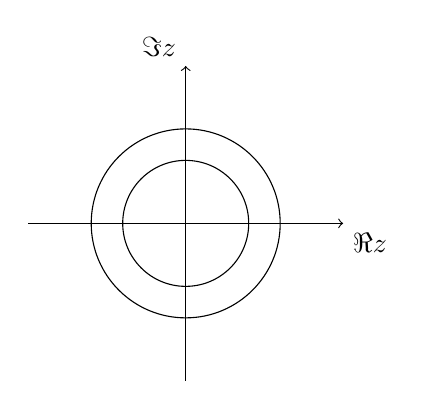
\begin{tikzpicture}[scale=1]
		\draw[->] (-2,0) -- (2,0) node[anchor=north west] {$\Re{z}$};
		\draw[->] (0,-2) -- (0,2) node[anchor=south east] {$\Im{z}$};
		\clip (-2,-2) rectangle (2,2);
		\draw (0,0) circle (1.2cm);
		\draw (0,0) circle (0.8cm);
		\end{tikzpicture}
	\end{center}
	Se per assurdo la serie converge in $z \implies$ per il teorema precedente  avremmo convergenza in ogni sfera con raggio minore di $\abs{\frac{1}{z}}$. e quindi anche in $w$ questo nega l'ipotesi.ASSURDO.
\end{proof}
\observation
Come è fatto l'insieme su cui si ha convergenza??\\
segue da queste due ultime proposizioni che se $\brackets{a_n:n\in\N}$ è una successione in $\C$ allora l'insieme $\brackets{z\in\C:\sum\limits_{n=0}^{+\infty}a_nz^n converge}$ è un cerchio.\\Sulla circonferenza non ci soffermaiamo a capire cosa accade poiché tutto può accadere.
\definition
Raggio di convergenza della serie $\sum\limits_{n=0}^{+\infty}a_nz^n\bydef \rho=\sup\brackets{r \geq 0 :\sum\limits_{n=0}^{+\infty}a_nz^n converge su B(0,r)}$
\observation
Il raggio di convergenza di una serie di potenze può essere $0$, un numero reale positivo o $+\infty$.
\observation
una definizione come $\rho=\inf\brackets{r \geq 0 :\sum\limits_{n=0}^{+\infty}a_nz^n non converge su B(0,r)}$ non sta in piedi poiché questo insieme potrebbe essere vuoto, mentre quello sopra non è mai vuoto, poerché $r=0$ c'è sempre poiché in $0$ si ha sempre convergenza. Ilsecondo potrebbe essere vuoto perché ci sono serie che convergono su tuttoil piano complesso e quindi non si avrebbe nessun $r$ fuori da quale non sia ha convergenza.\\
\proposition CRITERIO DELLA RADICE.\\
Data la serie di potenze $\sum\limits_{n=0}^{+\infty}a_nz^n$, sia $l=\lim\limits_{n\to+\infty}\sqrt[n]{\abs{a_n}}$.\\
Se questo limite esiste, allora il raggio di convergenza è
$\rho =
	\begin{cases}
		0				&	\text{se }l=+\infty\\
		\frac{1}{l} 	&	\text{se }l\in\left]0,+\infty\right[\\
		+\infty 		& 	\text{se }l=0
	\end{cases}
$
\proposition CRITERIO DEL RAPPORTO.\\
Data la serie di potenze $\sum\limits_{n=0}^{+\infty}a_nz^n$, sia $l=\lim\limits_{n\to+\infty}\frac{a_{n+1}}{a_n}$.\\
Se questo limite esiste, allora il raggio di convergenza è
$\rho =
\begin{cases}
0				&	\text{se }l=+\infty\\
\frac{1}{l} 	&	\text{se }l\in\left]0,+\infty\right[\\
+\infty 		& 	\text{se }l=0
\end{cases}
$
ESEMPIO::$e^z=\sum\limits_{n=0}^{+\infty}\frac{1}{n!}z^n$\\
$a_n=\frac{1}{n!} ...  \abs{\frac{a_{n+1}}{a_n}}=\frac{\frac{1}{(n+1)!}}{\frac{1}{n!}}=\frac{n!}{(n+1)!}=\frac{1}{n+1}\overset{n\to+\infty}{\to}0 \implies \rho=+\infty$\\
ESEMPIO::$sin(z)=\sum\limits_{n=0}^{+\infty}\frac{(-1)^nz^{2n+1}}{(2n+1)!}$ quindi
$a_n =
\begin{cases}
0		&	\text{se }n\text{ è pari}\\
...		&	\text{se }n\text{ è dispari}\\
\end{cases}
$\\
...\\
...\\
...\\
ESEMPIO::$sin(z)=\sum\limits_{n=0}^{+\infty}\frac{(-1)^nz^{2n}}{(2n)!}$ quindi
$a_n =
\begin{cases}
...		&	\text{se }n\text{ è pari}\\
0		&	\text{se }n\text{ è dispari}\\
\end{cases}
$\\
...\\
...\\
...\\
ESEMPIO:: $e^{iy}$ con $y\in \R$
\[e^{iy} = \sum\limits_{n=0}^{+\infty}\frac{1}{n!}(iy)^n = \sum\limits_{n=0}^{+\infty}\frac{1}{(2n)!}(iy)^{2n} + \sum\limits_{n=0}^{+\infty}\frac{1}{(2n+1)!}(iy)^{2n+1} = \]
\[ = \sum\limits_{n=0}^{+\infty}\frac{(-1)^n}{(2n)!}(y)^{2n} + i\sum\limits_{n=0}^{+\infty}\frac{(-1)^n}{(2n+1)!}(y)^{2n+1} = cos(y)+isin(y)\]
\begin{enumerate}
	\item $i^{2n}=\left(i^2\right)^n=(-1)^n$
	\item $i^{2n+1}=i\left(i^2\right)^n=i(-1)^n$
\end{enumerate}
ESEMPIO:: $e^{i\pi}+1=cos(\pi)+i\cdot sin(\pi)=0$\\
ESEMPIO:: $\sum\limits_{n=0}^{+\infty}z^n=\frac{1}{1-z}$ con $\rho=1$
ESEMPIO:: Sia $f(x)=\frac{1}{1+x^2}=\frac{1}{1-(-x^2)} = \sum\limits_{n=0}^{+\infty}(-x^2)^n=\sum\limits_{n=0}^{+\infty}(-1)^nx^{2n}$\\
QUI GRAFICO ..............\\
..........................\\
Questa serieconverge esclusivamente per $\abs{x}<1$, mentre la funzione $f$ è definita su tutto $ \R$, $f\in \cntclass{\infty}( \R; \R)$\\
In $\C$, lafunzione $f(z)=\frac{1}{1+z^2}$ è la somma della serie $\sum\limits_{n=0}^{+\infty}(-1)^nz^{2n}$ che ha raggio di convergenza  $\rho=1$. Infatti, $f(z)$ è singolare sia in $z=i$ sia in $z=-i$.\\
ALTRO GRAFICO::::::::::::::::\\
................................\\

\subsection{Serie di Taylor}
ESEMPIO:: $ln(1+z)$. Calcolare la Serie di Taylor.
\[D\left[ln(1+z)\right] = \frac{1}{1+z} = \sum\limits_{n=0}^{+\infty}(-1)^nz^n\]
\[\int \sum\limits_{n=0}^{+\infty}(-1)^nz^n dz = \sum\limits_{n=0}^{+\infty}\frac{(-1)^n}{n+1}z^{n+1}=\sum\limits_{n=1}^{+\infty}\frac{(-1)^{n-1}}{n}z^n\]
\begin{lemma}
	\label{lemma:taylor_rad_convergency}
	Sia $\brackets{a_n:n \in \N}$ una successione a valori in $\C$. Le serie:
	\[\sum_{n=0}^{+\infty} a_n z^n ,\qquad \sum_{n=1}^{+\infty} n a_n z^{n-1} \qquad\text{e}\qquad \sum_{n=0}^{+\infty} \frac{a_n}{n+1}z^{n+1}\]
	hanno lo stesso raggio di convergenza
	\begin{proof}
		Omessa
	\end{proof}
\end{lemma}

\definition
Sia $r\in \R$ con $r>0$. La funzione $f$ si dice analitica su $\left]-r,r\right[ \bydef f(x)=\sum\limits_{n=0}^{+\infty}a_nx^n \quad \forall x\in\left]-r,r\right[$ per opportuni $a_n\in \R$
\observation
In altre parole chiamiamo analitica una funzione che può essere scritta come somma di una serie di potenze convergente su $\left]-r,r\right[$ \\
ESEMPIO:: $x\to e^x$ è analitica su $ \R$\\
ESEMPIO:: $x\to\frac{1}{1+x^2}$ è analitica su $\left]-1,1\right[$\\
\proposition
Se $f$ è analitica su $\left]-r;r\right[$ per $r\in \R$ e $r>0 \implies f\in \cntclass{0}(\left]-r,r\right[; \R)$
\begin{proof}
	$f$ è analitica  allora posso scriverla come $f=\sum\limits_{n=0}^{+\infty}a_nx^n$ cioè la funzione è limite di una serie, se la serie converge totalmente allora converge uniformemente. Il limite uniforme di funzioni continue(in questo caso polinomi) è una funzione continua. cioè la $f$ è continua.
\end{proof}
\proposition PROP+PROOF\\
Sia $f:\left]-r,r\right[\to \R$ e $f$ analitica su $\left]-r,r\right[ \bydef f(x)=\sum\limits_{n=0}^{+\infty}a_nx^n \implies$ ho convergenza totale $\implies$ ho convergenza uniforme di funzioni continue
\[\implies f\in \cntclass{0}(\left]-r,r\right[; \R),\quad a_0=f(0)\]
La serie delle derivate $\sum\limits_{n=0}^{+\infty}na_nx^{n-1}$ converge totalmente su $\left]-r,r\right[$ cioè
\[\sum\limits_{n=0}^{+\infty}f'(x)=\sum\limits_{n=0}^{+\infty}na_nx^{n-1} \uconvarrow g\]
\[\sum\limits_{n=0}^{+\infty}fn(0)\to f(0), f_n\in ????????????\]
Allora la serie delle derivate converge alla derivata della serie
\[\implies \in \cntclass{1}(\left]-r,r\right[; \R),\quad a_1=f'(0)\]
Questo ragionmento può essere ripetuto:
\[\implies \forall k\in\N,\quad f\in \cntclass{k}(\left]-r,+r\right[),\quad a_k=k!f^{(k)}(0)\]
e analogamente
\[f\in \cntclass{\infty}(\left]-r,r\right[; \R),\quad f(x)=\sum\limits_{n=0}^{+\infty}\frac{1}{n!}f^{(n)}(0)x^n\]
\observation Qui abbiamo detto se $f$ è analitica $\implies \ldots$, vorrei fare un qualche tipo di viceversa per poter capire se $f$ è analitica o no.
\proposition
Sia $f:\left]-r,r\right[\to \R$
\begin{center}
	$\left.\begin{matrix}
	f\in \cntclass{\infty}(\left]-r,r\right[; \R)\\
	\sum\limits_{n=0}^{+\infty}\frac{1}{n!}f^{(n)}(0)x^n\text{ converge totalmente su } \left]-r,r\right[\\
	\end{matrix}\right\}\implies f$ è analitica  .....
\end{center}
Per avere $f$ analitica  necessariamente come ipotesi deve esserci $f\in \cntclass{\infty}$ e $f$ che si può scrivere come sviluppo in serie di Taylor,dalla proposizione precedente. Questo basta? NO\\
ESEMPIO:: $f(x)=\left\{\begin{matrix}0&& x=0\\e^{-\frac{1}{x^2}}&&x\ne 0\end{matrix}\right.$
\begin{center}
	\begin{tikzpicture}[scale=1]
	%\draw[->] (0,-4) -- (0,4) node[anchor=north west] {$x$};
	%\draw[->] (-0.1,0) -- (1.2,0) node[anchor=south east] {$y$};
	%\clip (-4,0) rectangle (4,1);
	%\draw[domain=-4:4,smooth,variable=\x] plot ({\x},{{-1/(\x*\x)}});
	\end{tikzpicture}
\end{center}
\begin{enumerate}
	\item $f\in \cntclass{\infty}( \R; \R)$
	\item $\sum\limits_{n=0}^{+\infty}\frac{1}{n!}f^{(n)}(0)x^n$ converge totalmente su $ \R$
	\item $f(x)\ne\sum\limits_{n=0}^{+\infty}\frac{1}{n!}f^{(n)}(0)x^n$
\end{enumerate}
\begin{enumerate}
	\item Vediamo se è $\cntclass{0}$, quindi calcolo $\lim\limits_{x\to 0^{+}}f(x)=\lim\limits_{x\to 0^{-}}f(x)=0=f(0)\implies f\in \cntclass{0}( \R; \R)$.\\
	Ora calcoliamo la derivata fuori dallo zero, ne facciamo il limite per $x\to 0$ da destra e da sinitra e vediamo cosa succede.\\
	Se $x\ne 0$, $f'(x)=\frac{2}{x^3}e^{-\frac{1}{x^3}}$ e $\lim\limits_{x\to 0^{+}}f'(x)=\lim\limits_{x\to 0^{-}} = 0 \implies f\in \cntclass{1}( \R; \R)$\\
	..........\\
	ancora una derivata.......\\
	..........\\
	Continuando a derivare  avremmo sempre un rapporto di polinomi che moltiplica un esponenziale, e l'esponenziale vince sempre. quindi fa $0$.
	itero il ragionamento......\\
	.......\\
	\item In (1) abbiamo visto  che tutte le derivate nello zero si annullavano, cioè
	\[\forall n\in\N, f^{(n)}(0)=0 \implies \sum\limits_{n=0}^{+\infty}\frac{1}{n!}f^{(n)}(0)x^n\]
	è la serie identicamente nulla  che banalmente converge totalmente su tutto $ \R$
	\item Anche osservandoil grafico è chiaro che la $f$ non è la funzione identicamente nulla cioè è diversa dal suo sviluppo in serie
	\[f(x)\ne\sum\limits_{n=0}^{+\infty}\frac{1}{n!}f^{(n)}(0)x^n\]
\end{enumerate}
Il Problema nasce dall'$o(x^n)$ che scriviamo alla fine dello sviluppo n-esimo di questa funzione, perché l'intorno in cui si ha $o(x^n)$ diventa sempre più piccolo.
GRAFICO...\\
GRAFICO...\\
Mandando l'ordine $n$ all'infinito, l'intervallo su cui si ha l'o piccolo tende a diventare un punto (lo zero). Quindi abbiamo l'ugualianza tra la funzione e il suo sviluppo solo nell'origine.????????NON COMPRESA????\\
????????NON COMPRESA????\\
????????NON COMPRESA????\\
????????NON COMPRESA????\\
Completiamo le ipotesi con la prossima proposizione:
\proposition
Sia $f:\left]-r,r\right[\to \R$
\begin{center}
	$\left.\begin{matrix}
	f\in \cntclass{\infty}(\left]-r,r\right[; \R)\\
	\exists H,K >0 :\forall n\in\N \sup\limits_{\left]-r,r\right[}\abs{f^{(n)}(x)} \leq HK^n\\
	\end{matrix}\right\}
	\implies f(x)=\sum\limits_{n=0}^{+\infty}\frac{1}{n!}f^{(n)}(0)x^n$
\end{center}
\observation
L'ipotesi centrale ............. qui non c'è
\observation
Sia $\sum\limits_{n=0}^{+\infty}(z,w)^n$ una serie di potenze in due variabili.\\
Quando abbiamo due variabili, non si può parlare di raggio di convergenza. Questa serie è una serie geometrica che converge sse $\abs{zw}<1$. è  difficile parlare di raggio di convergenza  perché essendo $z,w\in\C$, se per una variabile servono due dimensioni per due variabili servono quattro dimensioni , e anche se non riusciamo a fare il disegno è evidente che l'insieme su cui la serie converge non è un cerchio(sfera).
\begin{example}[Esempi di Sviluppi in serie di Taylor]
	\label{ex:tay_series_examples}
	\begin{description}
		\item $e^x=\sum\limits_{n=0}^{+\infty}\frac{1}{n!}x^n$
		\item $sin(x)=\sum\limits_{n=0}^{+\infty}\frac{(-1)^n}{(2n+1)!}x^{(2n+1)}$
		\item $sinh(x)=\sum\limits_{n=0}^{+\infty}\frac{1}{(2n+1)!}x^{(2n+1)}$
		\item $cos(x)=\sum\limits_{n=0}^{+\infty}\frac{(-1)^n}{(2n)!}x^{(2n)}$
		\item $cosh(x)=\sum\limits_{n=0}^{+\infty}\frac{1}{(2n)!}x^{(2n)}$
		\item $\frac{1}{1-x}=\sum\limits_{n=0}^{+\infty}x^n$
		\item $ln(1+x)=\sum\limits_{n=1}^{+\infty}\frac{(-1)^{n+1}}{n}x^n$
		\item $arctan(1+x)=\sum\limits_{n=0}^{+\infty}\frac{(-1)^{n}}{2n+1}x^{(2n+1)}$
		\item $\frac{1}{1+x^2}=\sum\limits_{n=0}^{+\infty}(-1)^nx^2n$
		\item $\sum\limits_{n=0}^{+\infty}\frac{1}{n^\lambda}=\left\{\begin{matrix}\text{converge sse } \lambda >1\\ \text{diverge sse } \lambda  \leq 1 \end{matrix}\right.$
		\item $\sum\limits_{n=0}^{+\infty}q^n=\left\{\begin{matrix}\text{converge sse } \abs{q}<1, S=\frac{1}{1-x}\\ \text{diverge sse } \abs{q}>1\text{ o }q=1\\\nexists \text{ sse } x=-1 \end{matrix}\right.$
	\end{description}
\end{example}
\begin{exercise}
	\label{ex:deriv_func_with_taylor}
	Determinare le derivate delle funzioni
	\begin{itemize}[noitemsep]
		\item $x \to \sin x$
		\item $x \to \cos x$
		\item $x \to e^x$
	\end{itemize}
	utilizzando \fullref{ex:tay_series_examples}, il \fullref{lemma:taylor_rad_convergency} ed il \fullref{coro:deriv_serie_e_serie_derivate}.
\end{exercise}

\subsection{Serie di Fourier}
\definition
Siano $A\subseteq \R$, $f:A\to \R$ e $T>0$, $f$ è $T$-periodica $\bydef \forall x\in A
\left\{\begin{matrix}
x+T\in A\\f(x+T)=f(x)
\end{matrix}\right. $\\


ESEMPIO:: $\lfloor x \rfloor = \text{ parte intera } = \max\brackets{k\in\mathbb{Z}:k \leq x}$
\[\lfloor \pi \rfloor=3, \quad \lfloor \sqrt{2} \rfloor = 1 \quad \lfloor -e \rfloor = -3 \]
\begin{center}
	\begin{tikzpicture}
		\draw[->] (-4,0) -- (4,0) node[anchor=north west] {$x$};
		\draw[->] (0,-4) -- (0,4) node[anchor=south east] {$y$};

		\foreach \num in {-3,...,3} {
			\draw[line width=0.25mm] (\num , \num) -- (\num+1 , \num);
			\draw[fill=black] (\num , \num) circle (0.1cm);
			\draw (\num+1, \num) circle (0.1cm);
		}
	\end{tikzpicture}
\end{center}
è $1$-periodica.
ESEMPIO:: $mant(x)=\text{ mantissa di x } = x- \lfloor x \rfloor$
\begin{center}
	\begin{tikzpicture}
	\draw[->] (-4,0) -- (4,0) node[anchor=north west] {$x$};
	\draw[->] (0,-4) -- (0,4) node[anchor=south east] {$y$};

	\foreach \num in {-3,...,3} {
		\draw[line width=0.25mm] (\num , 0) -- (\num+1 , 1);
		\draw[fill=black] (\num , 0) circle (0.1cm);
		\draw (\num+1, 1) circle (0.1cm);
	}
	\end{tikzpicture}
\end{center}
è $1$-periodica.
\observation
La funzione costante è $T$-periodica $\forall T>0$, ma non ha un periodo minimo, per questo motivo non la consideriamo.
\observation
Sia $f:A\to \R$ $T$-periodica. Allora possiamo definire $\overline{f}:\overline{A}\to \R$ che sia $2\pi$-periodica data da:
\[x\to f\left(\frac{T}{2\pi}x\right),\quad \overline{A}=\frac{2\pi}{T}A\]
\proposition
Siano $A\subseteq \R$, $f:A\to \R$ e $T>0$\\
$f$ è $T$-periodica $\implies \forall n\in\N$, $f$ è $nT$-periodica.
\proposition
Sia $f:\left[0,2\pi\right[\to \R \implies \exists ! \hat{f}: \R\to \R$ t.c.: $\left\{\begin{matrix} \hat{f} 2\pi-periodica\\\hat{f}_{\left|\left[0,2\pi\right]\right.}=f\end{matrix}\right.$
\begin{proof}
	$\forall x\in \R. \exists ! \hat{x}\in\left[0,2\pi\right[$ t.c.: $x=2\pi\cdot k+\hat{x}$ con $k\in\mathbb{Z}$ e $k=\left[??????\right]$
	\[\hat{f}(x)=f(\hat{x})\]
\end{proof}
cioè se noi estendiamo una funzione definita su $\left[0,2\pi\right[$ a tutto $ \R$ otteniamo una funzione unica e periodica.
\observation
Con i polinomi di Taylor ........\\
........\\
........\\
........\\
........\\
........\\
\definition
Dati $2n+1$ numeri reali $a_0,a_1,\dotsc,a_n,b_1,\dotsc,b_n$ si dice polinomio trigonometrico di coefficienti $a_0,a_1,\dotsc,a_n,b_1,\dotsc,b_n$ la funzione:
\[\begin{array}{rcl} p: \left[-\pi,\pi\right] & \to &  \R \\ x & \to & \frac{a_0}{2}+\sum\limits_{k=1}^{N}\left(a_ncos(nx)+b_nsin(nx)\right) \end{array}\]
\observation
Essendo un'approssimazione, si deve aggiungere l'errore. Come è fatto?. Per far uscire conti giusti e comodi andrebbe usata la distanza quadratica , ma questo prevede una lunga parte introduttiva, noi allora lo stimiamo con la distanza infinita.
\definition
Date due successioni di numeri reali $\brackets{a_n:n\in\N}$,$\brackets{b_n:n\in\N\setminus\brackets{0}}$, si defininisce serie trigonometrica di coefficienti  $\brackets{a_n:n\in\N}$,$\brackets{b_n:n\in\N\setminus\brackets{0}}$ la serie
\[\begin{array}{rcl} \mathfrak{F}: \left[-\pi,\pi\right] & \to &  \R \\ x & \to & \frac{a_0}{2}+\sum\limits_{k=1}^{+\infty}\left(a_ncos(nx)+b_nsin(nx)\right) \end{array}\]
LEMMA::\\
Se $h,k\in\N$ valgono le seguenti uguaglianze:
\begin{description}
	\item[$\ast$]
	$\int_{-\pi}^{\pi} cos(hx)cos(kx)=
	\left\{\begin{matrix}
	0 &&h\ne k\\\pi&&0\ne h=k\\2\pi&&0=h=k
	\end{matrix}\right.$
	\item[$\ast$] $\int_{-\pi}^{\pi}cos(hx)sin(kx)= 0 $
	\item[$\ast$]
	$\int_{-\pi}^{\pi}sin(hx)sin(kx)=
	\left\{\begin{matrix}
	0 &&h\ne k\text{ oppure }h=k=0\\ \pi&&0\ne h=k
	\end{matrix}\right.$
\end{description}
ESERCIZIO:: IL POLINOMIO DI FOURIER FORNISCE LA MIGLIORE APPROSSIMAZIONE NEL SENSO DELLA DISTANZA QUADRATICA.\\
Sia $f: \intervalclose{-\pi}{\pi} \to \R$, quale è la funzione a lei più vicina nel senso della distanza quadratica?\\
Fisso $N\in\N$ e prendo il polinomio trigonometrico di grado $N$
\[p_N(x)=\trigonpol{n}{1}{N}\]
con $a_0,a_1,\dotsc,a_n,b_1,\dotsc,b_n\in \R$, il problema è quello di minimizzare $d_2(f,p_n)$ quindi un problema di minimo. Stiamo cercando i coefficienti del polinomio trigonometrico quindi studiamo una funzione $\varphi(a_0,a_1,\dotsc,a_N,b_1,\dotsc,b_N) = \sqrt{\int_{-\pi}^{\pi}\left[f(x)-p_n(x)\right]^2}\integrald{x}$.\\
Essendo la funzione radice quadrata monotona crescente ne studiamo solo il radicando:
\[\varphi(a_0,a_1,\dotsc,a_N,b_1,\dotsc,b_N)=\int_{-\pi}^{\pi}\left[\trigonpol{n}{1}{N}-f(x)\right]^2dx\]
\observation
con $f\in \cntclass{1}$:
\[F(\alpha,\beta,x)=\int_{\alpha}^{\beta}f(x,t)\integrald{t}\]
\[\partial_\alpha F(\alpha,\beta,x)=-f(x,\alpha)\integrald{t}\]
\[\partial_\beta F(\alpha,\beta,x)=f(x,\beta)\integrald{t}\]
\[\nabla_x F(\alpha,\beta,x)=\int_{\alpha}^{\beta}\nabla_xf(x,t)\integrald{t}\]
Qudindi applicando al nostro caso otteniamo
\[\partial_{a_0}\varphi = \int_{-\pi}^{\pi}\partial_{a_0}\left(\left[\trigonpol{n}{1}{N}-f(x)\right]^2\right)\integrald{x}=\]
\[ = \int_{-\pi}^{\pi} \frac{1}{2}2\left(\trigonpol{n}{1}{N}-f(x)\right)\integrald{x}=\]
\[ =  \int_{-\pi}^{\pi} \frac{a_0}{2}\integrald{x} + \]
\[\int_{-\pi}^{\pi} a_1cos(x)\integrald{x} +
\ldots +
\int_{-\pi}^{\pi} a_Ncos(Nx)\integrald{x} + \]
\[\int_{-\pi}^{\pi} b_1sin(x)\integrald{x} +
\ldots +
\int_{-\pi}^{\pi} b_Nsin(Nx)\integrald{x} - \]
\[ \int_{-\pi}^{\pi} f(x)\integrald{x} = \]
L'integrale di una sinusoide su un multiplo intero del periodo è $0$ quindi
\[=\pi a_0-\int_{-\pi}^{\pi}f(x)\integrald{x}\]
Calcolando direttamente anche le derivate seconde si ottiene che
\[\partial^2_{a_0a_0}=\pi\quad\partial^2_{a_0a_n}=0\quad\partial^2_{a_0b_n}=0\quad\forall n=1,\dotsc,N\]

\[\partial_{a_k}\varphi = \int_{-\pi}^{\pi}\partial_{a_k}\left(\left[\trigonpol{n}{1}{N}-f(x)\right]^2\right)\integrald{x}=\]
\[ = \int_{-\pi}^{\pi} 2cos(kx) \left[\trigonpol{n}{1}{N}-f(x)\right]\integrald{x}=\]
\[ =  \cancel{\int_{-\pi}^{\pi} a_0cos(kx)\integrald{x}} + \]
\[\cancel{\int_{-\pi}^{\pi} 2a_1cos(x)cos(kx)\integrald{x}} +
\ldots +
\int_{-\pi}^{\pi} 2a_kcos(kx)cos(kx)\integrald{x}
\ldots +
\cancel{\int_{-\pi}^{\pi} 2a_Ncos(Nx)cos(kx)\integrald{x}} + \]
\[\cancel{\int_{-\pi}^{\pi} 2b_1sin(x)cos(kx)\integrald{x}} +
\ldots +
\cancel{\int_{-\pi}^{\pi} 2b_ksin(kx)cos(kx)}\integrald{x}
\ldots +
\cancel{\int_{-\pi}^{\pi} 2b_Nsin(Nx)cos(kx)\integrald{x}} - \]
\[\int_{-\pi}^{\pi} 2f(x)cos(kx)\integrald{x} = \]
E anche applicando il lemma
\[=2\pi\left[a_k-\int_{-\pi}^{\pi}f(x)cos(kx)\integrald{x}\right]\]
Calcolando direttamente anche le derivate seconde si ottiene che
\[\partial^2_{a_ka_0}=\pi\quad\partial^2_{a_ka_n}=
\left\{\begin{matrix}
0&&n\ne k\\2\pi&&n=k
\end{matrix}\right.
\quad\partial^2_{a_kb_n}=0\quad\forall n=1,\dotsc,N\]

\[\partial_{b_k}\varphi = \int_{-\pi}^{\pi}\partial_{b_k}\left(\left[\trigonpol{n}{1}{N}-f(x)\right]^2\right)\integrald{x}=\]
\[ = \int_{-\pi}^{\pi} 2sin(kx) \left[\trigonpol{n}{1}{N}-f(x)\right]\integrald{x}=\]
\[ =  \cancel{\int_{-\pi}^{\pi} a_0sin(kx)\integrald{x}} + \]
\[\cancel{\int_{-\pi}^{\pi} 2a_1cos(x)sin(kx)\integrald{x}} +
\ldots +
\cancel{\int_{-\pi}^{\pi} 2a_kcos(kx)sin(kx)}\integrald{x}
\ldots +
\cancel{\int_{-\pi}^{\pi} 2a_Ncos(Nx)sin(kx)\integrald{x}} + \]
\[\cancel{\int_{-\pi}^{\pi} 2b_1sin(x)sin(kx)\integrald{x}} +
\ldots +
\int_{-\pi}^{\pi} 2b_ksin(kx)sin(kx)\integrald{x}
\ldots +
\cancel{\int_{-\pi}^{\pi} 2b_Nsin(Nx)sin(kx)\integrald{x}} - \]
\[\int_{-\pi}^{\pi} 2f(x)sin(kx)\integrald{x} = \]
E anche applicando il lemma
\[=2\pi\left[b_k-\int_{-\pi}^{\pi}f(x)cos(kx)\integrald{x}\right]\]
Calcolando direttamente anche le derivate seconde si ottiene che
\[\partial^2_{b_ka_0}=\pi\quad\partial^2_{b_ka_n}=
\left\{\begin{matrix}
0&&n\ne k\\2\pi&&n=k
\end{matrix}\right.
\quad\partial^2_{b_kb_n}=0\quad\forall n=1,\dotsc,N\]
Si verifica la condizione $\nabla\varphi = 0$ con
\begin{description}
	\item[$\ast$] $a_0=\frac{1}{\pi}\int_{-\pi}^{\pi}f(x)\integrald{x}$
	\item[$\ast$] $a_k=\frac{1}{\pi}\int_{-\pi}^{\pi}f(x)cos(kx)\integrald{x}$
	\item[$\ast$] $b_k=\frac{1}{\pi}\int_{-\pi}^{\pi}f(x)sin(kx)\integrald{x}$
\end{description}
La matrice Hessiana di $\varphi$ risulta \[H_{\varphi}=\left[\begin{matrix}
\pi&&0&&0&&\ldots&&0\\
0&&2\pi&&0&&\ldots&&0\\
0&&0&&2\pi&&\ldots&&0\\
\vdots&&\vdots&&\vdots&&\ddots&&\vdots\\
0&&0&&0&&0\ldots&&2\pi
\end{matrix}\right]\]
è una matrice diagonale quindi si leggono direttamente tutti gli autovalori che sono strettamente positivi quindi la forma quadratica è definita positiva ed il punto in questione è un punto di minimo assoluto.
\definition
Sia $f: \intervalclose{-\pi}{\pi} \to \R$, i coefficienti di Fourier di $f$ sono (ovviamente $f$ deve essere tale da ammetterli finiti):
\[a_0=\frac{1}{\pi}\int_{-\pi}^{\pi}f(x)\integrald{x}\]
\[a_k=\frac{1}{\pi}\int_{-\pi}^{\pi}f(x)cos(kx)\integrald{x}\quad k\in\N\setminus{\brackets{0}}\]
\[b_k=\frac{1}{\pi}\int_{-\pi}^{\pi}f(x)sin(kx)\integrald{x}\quad k\in\N\setminus{\brackets{0}}\]
La serie di Fourier di $f$ è
\[\trigonpol{k}{1}{+\infty}\]
\proposition
Sia $F: \intervalclose{-\pi}{\pi} \to \R$ la somma della serie trigono metrica definita dai coefficienti $\brackets{a_n:n\in\N}$ e $\brackets{a_n:n\in\N\setminus\brackets{0}}$ e la serie trigonometrica converge uniformemente allora $F$ è una funzione continua e
\[a_k=\frac{1}{\pi}\int_{-\pi}^{\pi}F(x)cos(kx)\integrald{x}\quad k\in\N\]
\[b_k=\frac{1}{\pi}\int_{-\pi}^{\pi}F(x)sin(kx)\integrald{x}\quad k\in\N\setminus{\brackets{0}}\]
ESEMPIO+DIMOSTRAZIONE:::\\
sia $f(x)=\trigonpol{n}{1}{+\infty}$. Allora:\\
\[a_0=\frac{1}{\pi}\int_{-\pi}^{\pi}f(x)\integrald{x}=\frac{1}{\pi}\int_{-\pi}^{\pi}\trigonpol{n}{1}{+\infty}\integrald{x}=\]
\[
= \frac{1}{\pi}\int_{-\pi}^{\pi}\frac{a_0}{2} +
\frac{1}{\pi}\int_{-\pi}^{\pi}\left(\sum\limits_{n=1}^{+\infty} a_ncos(nx)\right)\integrald{x} +
\frac{1}{\pi}\int_{-\pi}^{\pi}\left(\sum\limits_{n=1}^{+\infty} b_ncos(nx)\right)\integrald{x}
\]
Poiché si ha convergenza uniforme si può portare l'integrale dentro la sommatoria.
\[
= \frac{1}{\pi}\int_{-\pi}^{\pi}\frac{a_0}{2} +
\cancel{\frac{1}{\pi}\sum\limits_{n=1}^{+\infty}\int_{-\pi}^{\pi} a_ncos(nx)\integrald{x}} +
\cancel{\frac{1}{\pi}\sum\limits_{n=1}^{+\infty}\int_{-\pi}^{\pi} b_ncos(nx)\integrald{x}}=
\]
\[=\frac{1}{\pi}\frac{a_0}{2}\left(\pi-(-\pi)\right)=a_0\]


\[a_k=\frac{1}{\pi}\int_{-\pi}^{\pi}f(x)cos(kx)\integrald{x}=\]
\[\frac{1}{\pi}\left[
\cancel{\int_{-\pi}^{\pi}\frac{a_0}{2}cos(kx)\integrald{x}}+
\int_{-\pi}^{\pi}\left(\sum\limits_{n=1}^{+\infty}a_ncos(nx)cos(kx)\right)\integrald{x}+
\cancel{\int_{-\pi}^{\pi}\left(\sum\limits_{n=1}^{+\infty}b_nsin(nx)cos(kx)\right)\integrald{x}}
\right]=\]
\[\frac{1}{\pi}\left[
\cancel{\int_{-\pi}^{\pi}\left(\sum\limits_{n=1}^{k-1} a_ncos(nx)cos(kx)\right)\integrald{x}}+
\int_{-\pi}^{\pi}a_kcos(kx)cos(kx)\integrald{x}+
\cancel{\int_{-\pi}^{\pi}\left(\sum\limits_{n=k+1}^{+\infty}a_ncos(nx)cos(kx)\right)}\integrald{x}
\right]=\]
\[=\frac{1}{\pi}\pi a_k=a_k\]

\[b_k=\frac{1}{\pi}\int_{-\pi}^{\pi}f(x)sin(kx)\integrald{x}=\]
\[\frac{1}{\pi}\left[
\cancel{\int_{-\pi}^{\pi}\frac{a_0}{2}sin(kx)\integrald{x}}+
\int_{-\pi}^{\pi}\left(\sum\limits_{n=1}^{+\infty}a_ncos(nx)sin(kx)\right)\integrald{x}+
\cancel{\int_{-\pi}^{\pi}\left(\sum\limits_{n=1}^{+\infty}b_nsin(nx)sin(kx)\right)\integrald{x}}
\right]=\]
\[\frac{1}{\pi}\left[
\cancel{\int_{-\pi}^{\pi}\left(\sum\limits_{n=1}^{k-1} a_ncos(nx)sin(kx)\right)\integrald{x}}+
\int_{-\pi}^{\pi}a_kcos(kx)sin(kx)\integrald{x}+
\cancel{\int_{-\pi}^{\pi}\left(\sum\limits_{n=k+1}^{+\infty}a_ncos(nx)sin(kx)\right)}\integrald{x}
\right]=\]
\[=\frac{1}{\pi}\pi b_k=b_k\]
\observation
Se $d_2(f,\text{polinomio di Fourier})$ \`{e} minima $\implies$ il polinomio di Fourier \`{e} costruito con i coefficienti di Fourier di $f$.
\observation
Se $f$ \`{e} somma di una serie di funzioni $\implies$ i coefficienti della serie sono i coefficienti di Fourier.
\observation
Funzioni diverse possono avere gli stessi coefficienti di Fourier, cio\`{e} $\exists f,g$ con $f\ne g$ ma $f$ e $g$  hanno gli stessi coefficienti di Fourier.
ESEMPIO::
\begin{center}
	\begin{tikzpicture}
		\draw[->] (-2,0) -- (2,0) node [anchor=north west]{$x$};
		\draw[->] (0,0) -- (0,2);
		\clip (-2,0) rectangle (2,2);
		\draw[domain=-2:2,smooth,red,variable=\x] plot ({\x},{1}) node{$f$};
		\draw[domain=-2:2,smooth,blue,variable=\x] plot ({\x},{1}) node{$g$};
	\end{tikzpicture}
	SISTEMARE,
\end{center}
\observation
I coefficienti di Fourier non possono identificare univocamente puntualmente una funzione.
\subsubsection{Punto Di Vista Geometrico}
In $R^2$ Ci sono $2$ vettori $\hat{i},\hat{j}$ della base, se $\underline{v}\in \R^2 \implies \underline{v}=v_1\cdot \hat{i}+v_2\cdot \hat{j}$ con $v_1,v_2$ componenti di $\underline{v}$\\
Calcolo delle componenti:
\[\underline{v}\cdot \hat{i} = v_1\cdot \hat{i\cdot }\hat{i}+v_2\cdot \hat{j}\cdot \hat{i}=v_1\]
\[\underline{v}\cdot \hat{j} = v_1\cdot \hat{i}\cdot \hat{j}+v_2\cdot \hat{j}\cdot \hat{j}=v_2\]
Questo vale perché $\hat{i},\hat{j}$ è una base ortonormale.
In $R^3$ Ci sono $3$ vettori $\hat{i},\hat{j},\hat{k}$ della base, se $\underline{v}\in \R^3 \implies \underline{v}=v_1\hat{i}+v_2\hat{j}+v_3\hat{k}$ con $v_1,v_2,v_3$ componenti di $\underline{v}$\\
Calcolo delle componenti:
\[ v_1=\underline{v}\cdot \hat{i}\quad v_2=\underline{v}\cdot \hat{j}\quad v_3=\underline{v}\cdot \hat{k}  \]
In $R^n$ Ci sono $n$ vettori $e_1,e_2,\dotsc,e_n$ della base, se $\underline{v}\in \R^n \implies \underline{v}=v_1\cdot e_1+v_2\cdot e_2+\ldots+v_n\cdot e_n=\sum\limits_{k=1}^{n}v_k\cdot e_k$ con $v_1,v_2,\dotsc,v_n$ componenti di $\underline{v}$\\
Calcolo delle componenti:
\[v_k=\underline{v}\cdot e_k\]
\\
Con le Serie di Fourier su esegue la stessa operazione sullo spazi $\cntclass{0}(\intervalclose{-\pi}{\pi}; \R)$. Come elementi di base si ha un insieme di funzioni:
\begin{enumerate}
	\item $c_0:x\to 1$
	\item $c_1:x\to cos(x)$
	\item $c_2:x\to cos(2x)$
	\item $\ldots$
	\item $c_n:x\to cos(nx)$
	\item $s_1:x\to sin(x)$
	\item $s_2:x\to sin(2x)$
	\item $\ldots$
	\item $s_n:x\to sin(nx)$
\end{enumerate}
Si possono osservare due cose:
\begin{enumerate}
	\item Sono tutte funzioni linearmente indipendenti, poiché l'unica combinazione lineare di questi elementi che da l'elemento nullo è quella a coefficenti tutti nulli.
\end{enumerate}
\definition
Il prodotto scalare in $\cntclass{0} \bydef \left<f,g\right>=\int_{-\pi}^{\pi}f(x)g(x)\integrald{x}$
Altre simbologie usate sono: $ f\bullet g $, $(f|g)$
\observation linearità
\[\left<(\alpha\cdot f+\beta\cdot g), h \right>= \int_{-\pi}^{pi} (\alpha\cdot f(x)+\beta\cdot g(x))\cdot h(x) \integrald{x}=\]
\[=\int_{-\pi}^{pi} \left[\alpha\cdot f(x)\cdot h(x)+\beta\cdot g(x)\cdot h(x) \right]\integrald{x}= \]
\[=\alpha\int_{-\pi}^{pi} \cdot f(x)\cdot h(x) \integrald{x}+\beta\int_{-\pi}^{pi} \cdot g(x)\cdot h(x) \integrald{x} =\]
\[\alpha\left<f,h\right>+\beta\left<g,h\right>\]

Ripetiamolo stesso ragionamento applicato in $ \R^2, \R^3,$ e $ \R^n$ per ricavare le componenti, possiamo fare questo perché abbiamo una base e abbiamo definito un prodotto scalare.\\
Se $f(x)=\trigonpol{n}{1}{+\infty} \implies $
\[a_0=\frac{1}{\pi}\int_{-\pi}^{\pi}f(x)dxs=\frac{1}{\pi}\left<f,c_0\right> \]
\[a_k=\frac{1}{\pi}\int_{-\pi}^{\pi}f(x)cos(kx)\integrald{x}=\frac{1}{\pi}\left<f,c_k\right> \]
\[b_k\frac{1}{\pi}\int_{-\pi}^{\pi}f(x)sin(kx)\integrald{x}=\frac{1}{\pi}\left<f,s_k\right>\]
Quindi come prima le componenti di un vettore si ottengono moltiplicando(prodotto scalare) il vettore per gli elementi della base.\\
PER IL LEMMA:\\
\[
\left<c_h,c_k\right>=
\left\{\begin{matrix}
0&&h\ne k\\
2\pi&&0=h=k\\
\pi&&0\ne h=k\\
\end{matrix}\right.
\]
\[ \left<c_h,s_k\right>=0\]
\[
\left<s_h,s_k\right>=
\left\{\begin{matrix}
0&&h\ne k\\
\pi&&0\ne h=k\\
\end{matrix}\right.
\]
Il prodotto scalare di elementi diversi è nullo quindi la base è ortogonale, ma non è ortonormale in quanto il prodotto scalare tra due elementi diversi della base non è unitario.(ecco perché gli $\frac{1}{\pi})$ e $\frac{a_0}{2}$)\\
In generale in geometria non è difficile normalizzare una base, è sufficiente dividere tutti gli elementi per la loro norma. In questo caso decidiamo di non applicare questo ragionamento poiché la norma vale $\sqrt{\pi}$ e se normalizziamo dobbiamo aggiungere questo termini ......\\
Il prodotto scalare in $\cntclass{0}$ è molto legato alla $d_2$ infatti:
\[\norm{f}_2=\sqrt{\left<f,f\right>}=\sqrt{\int_{-\pi}^{\pi}f(x)\cdot f(x)\integrald{x}}\sqrt{\int_{-\pi}^{\pi}\left[f(x)\right]^2dx}\]
Continuano le analogie:\\
In $ \R^2$ ........\\
In $ \R^3$ .........\\
.....\\
......\\
......\\
.....\\
Passando in dimensione infinita, abbiamo una funzione $f$ (come vettore $\underline{v}$) nello spazio, e fare il polinomio di Fourier  vuole dire proiettare la funzione $f$ in uno spazio fatto dai primi $2n+1$ elementi della base che è uno spazio di dimensione finita.\\
\\
Esempio:::: Non ogni funzione ammette coefficienti di Fourier finiti. La funzione
\[\begin{array}{rcl} f: \left[-\pi,\pi\right] & \to &  \R \\
x & \to & \left\{\begin{matrix} 0 && x=0\\\frac{1}{x^2}&&x\ne 0 \end{matrix}\right. \end{array}\]
non ammette coefficienti di Fourier finiti.\\
Esempio::: Una funzione può ammettere tutti i coefficienti di Fourier finiti ed una serie di Fourier convergente, ma ad un limite diverso da $f$.La funzione.
\[\begin{array}{rcl} f: \left[-\pi,\pi\right] & \to &  \R \\
x & \to & \left\{\begin{matrix} -1 && x<0\\1&&x>0 \end{matrix}\right. \end{array}\]
ha coefficienti di Fourier
\[a_k=0\quad\forall k,\quad\quad \left\{\begin{matrix}0 && k\text{ dispari }\\ \frac{4}{k\pi}&& k \text{ pari } \end{matrix}\right.\]
e serie di Fourier
\[ F_f(x)= \frac{4}{\pi}\sum\limits_{k=0}^{+\infty}\frac{sin(2h+1)x}{2h+1} \]
questa serie converge puntualmente in $0$ ma $F_f(0)\ne f(0)$\\

ESEMPIO:: Due funzioni diverse possono avere gli stessi coefficienti di Fourier:
\[\begin{array}{rcl} f: \left[-\pi,\pi\right] & \to &  \R \\
x & \to & \left\{\begin{matrix} -1 && x<0\\0&&x= 0\\1&&x>0 \end{matrix}\right.\end{array}\]
\[\begin{array}{rcl} g: \left[-\pi,\pi\right] & \to &  \R \\
x & \to & \left\{\begin{matrix} -1 && x<0\\\pi&&x= 0\\1&&x>0 \end{matrix}\right.\end{array}\]
\observation
Sia $f$ una funzione pari $\implies bn=0 \forall n=1,2,\dotsc,+\infty$
\observation
Sia $f$ una funzione dispari $\implies an=0 \forall n=0,1,,\dotsc,+\infty$
\observation
Siano
\[f(x)=\frac{a_0}{2}+\sum\limits_{n=}^{+\infty}\left(a_ncos(nx)+b_nsin(nx)\right)\]
\[\varphi(x)=\frac{\alpha_0}{2}+\sum\limits_{n=}^{+\infty}\left(\alpha_ncos(nx)+\beta_nsin(nx)\right)\]
Allora
\[ F(x)=(f+\varphi)(x)=\frac{A_0}{2}+\sum\limits_{n=}^{+\infty}\left(A_ncos(nx)+B_nsin(nx)\right)\]
con $A_n=a_n+\alpha_n$. $B_n=b_n+\beta_n$.
cioè i coefficienti di Fourier dipendono linearmente dalla funzione.\\
Esempio::: $B_3=\frac{1}{\pi}\int_{-\pi}^{\pi}F(x)sin(3x)\integrald{x}=\frac{1}{\pi}\int_{-\pi}^{\pi}(f(x)+\varphi(x))sin(3x)\integrald{x}=$\\
$\frac{1}{\pi}\left[\int_{-\pi}^{\pi}f(x)sin(3x)\integrald{x}+\int_{-\pi}^{\pi}\varphi(x)sin(3x)\integrald{x}\right]=b_3+\beta_3$\\
Sia $f(x)=\frac{a_0}{2}+\sum\liminf_{n=1}^{+\infty}\left(a_ncos(nx)+b_ncos(nx)\right)$ allora $F=4f=\frac{A_0}{2}+\sum\limits_{n=1}^{+\infty}\left(A_ncos(nx)+B_ncos(nx)\right)$ con $A_n=4a_n$, $B_n=4b_n$\\
ESEMPIO
Esempio:::$B_3=\frac{1}{\pi}\int_{-\pi}^{\pi}F(x)sin(3x)\integrald{x}=\frac{1}{\pi}\int_{-\pi}^{\pi}4f(x)sin(3x)\integrald{x}=4b_3$\\
\begin{definition}[Funzione Continua a Tratti]
	Siano $a,b\in \R$ con $a<b$, una funzione $f:\intervalclose{a}{b} \to \R$. Allora $f$ è \textbf{continua a tratti} se esiste un numero finito di punti $x_1,x_2,\dotsc,x_n$ tali che:
	\begin{enumerate}
		\item In ogni punto di $\intervalclose{a}{b}\setminus\brackets{x_1,x_2,\dotsc,x_n}$ f è continua
		\item $i=1,2,\dotsc,n$ esistono finiti entrambi i limiti:
		\[\lim\limits_{x\to x_i^{-}}f(x)\quad \lim\limits_{x\to x_i^{+}}f(x)\]
	\end{enumerate}
\end{definition}

\observation
Dato $A\subseteq \R$ e data una funzione $f:A \to \R$, se $x_0$ è punto interno ad $A$, è comoda la notazione
\[f(x-)=\lim\limits_{\xi\to x^{-}}f(\xi)\quad f(x+)=\lim\limits_{\xi\to x^{+}}f(\xi)\]
Ovviamente se $f$ è continua in $x$ allora $f(x-)=f(x)=f(x+)$
ESEMPIII:::\\
GRAFICO::::\\
GRAFICO::::\\
.......\\
.......\\
.......\\
.......\\
\proposition
Sia $f: \intervalclose{-\pi}{\pi} \to \R$, $f$ è continua a tratti $\implies$ esistono finiti tutti i coefficienti di Fourier di $f$
\proposition
Sia $f: \intervalclose{-\pi}{\pi} \to \R$,\\
-$f$ è continua a tratti\\
-$\forall \overline{x} \in\intervalclose{-\pi}{\pi}$, esistono finiti:\\
\[ \lim\limits_{x\to\overline{x}^{-}}=\frac{f(x)-f(\overline{x}-)}{x-\overline{x}} \]
\[ \lim\limits_{x\to\overline{x}^{+}}=\frac{f(x)-f(\overline{x}+)}{x-\overline{x}} \]
Allora:\\
La serie di Fourier di $f$ converge puntualmente in $\overline{x}$ e $F_f(\overline{x})=\frac{f(\overline{x}-)-\overline{x}+}{2}$ (che è il punto medio del salto.)
\observation NIENTE CUSPIDI E NIENTE TANGENZE VERTICALI.

\corollary
Sia $f: \intervalclose{-\pi}{\pi} \to \R$,\\
$f$ è continua a tratti.\\
Sia $\overline{x}\in\intervalclose{-\pi}{\pi}$ un punto in cui $f$ è derivabile. Allora la serie di Fourier $F_f$ di $f$ converge in $\overline{x}$ e $F_f(\overline{x})=f(\overline{x})$
\proposition
Sia $f: \intervalclose{-\pi}{\pi} \to \R$.Se:\\
\begin{description}
	\item[$\ast$] $f\in \cntclass{0}(\intervalclose{-\pi}{\pi}; \R)$
	\item[$\ast$] $\exists x_1,x_2,\dotsc,x_n\in\intervalclose{-\pi}{\pi}$ t.c.:
	\begin{description}
		\item[-] $f$ è derivabile in $x$
		\item[-] $f'$ continua in $x$
	\end{description}
	\item[$\ast$] $\forall i=1,2,\dotsc,n$ e $\forall x\in\intervalclose{-\pi}{\pi}$ esistono finiti
	\[\lim\limits_{x\to x_i^{-}}\frac{f(x)-f(x_i-)}{x-x_i}\qquad \lim\limits_{x\to x_i^{+}}\frac{f(x)-f(x_i+)}{x-x_i}\]

\end{description}
Allora\\
La serie di Fourier $F_f$ di $f$ converge a $f$ uniformemente su $\intervalclose{-\pi}{\pi}$
\corollary
Sia $f: \intervalclose{-\pi}{\pi} \to \R$, e $f\in \cntclass{1}(\intervalclose{-\pi}{\pi}; \R)$.\\
Allora la serie di Fourier di $F_f$ di $f$ converge uniformemente a $f$ su $\intervalclose{-\pi}{\pi}$.
\part{Equazioni Differenziali}
\chapter{Equazioni Differenziali}
\section{Preliminari}
Equazione è un uguaglianza in cui c'è almeno una incognita.\\
Equazione differenziale è un particolare tipo di equazione e stabilisce una relazione tra la funzione incognita e le sue derivate.In un equazione funzionale si cerca l'uguaglianza di: insieme di arrivo, insieme di partenza, corrispondenza.\\
Non è necessario sapere il valore della soluzione ma sapere che ne esiste una.????????\\\\
Equazione differenziale ordinaria:\\
1- La funzione incognita è funzione di una sola variabile, solitamente il tempo.\\
2- La funzione incognita e le sue derivate sono calcolate allo stesso istante di tempo.\\
\definition\label{def:equaz_diff}
Si dice equazione differenziale ordinaria di ordine $n$ nella funzione incognita $x\in \R^k$ un espressione del tipo:
$$f(t,x, x',\ldots,x^{(n)})=0$$
dove $f:A\to \R^m$, $A\subseteq \R^{1+(1+n)k}$ e $t\in \R$.\\
$m$ e $k$ caratterizzano il problema e son dunque libere. La dimensione di partenza $1+(1+n)k$ del problema è obbligata e dovuta alla somma di:
\begin{itemize}
	\item $1 = dim(t)$
	\item $(1+n)k$
	\begin{itemize}
		\item $(1+n)$ il numero totale delle funzioni: $n$ derivate ed $x$ stessa
		\item $k$ la dimensione dell'insieme di partenza di ogni funzione incognita
	\end{itemize}
\end{itemize}
Soluzione di questa equazione differenziale è una qualunque funzione $x:I\to \R^k$ definita su un intervallo $I\subseteq \R$, derivabile $n$ volte in $I$ e tale che $\forall t\in I$\\
$$(t,x, x',\ldots,x^{(n)}) \in A$$
$$f(t,x, x',\ldots,x^{(n)})=0$$
Soluzione massimale  di un equazione differenziale ordinaria è una soluzione $x_m:I_m\to \R^k$ tale che nessuna soluzione possa essere definita in un intervallo $I$ con $I_m\subseteq I$
\begin{note}
	Un'equazione differenziale ammette, in generale, infinite soluzioni.
\end{note}
\begin{note}
	\hypertarget{note:diff_eq_sol_definition_set}
	La soluzione di un'equazione differenziale può, analiticamente, essere definita su un intervallo $J\supset I$ ($I$ intervallo di definizione della funz. differenziale $f$). Non ha però senso considerare il suo comportamento al di fuori di $I$, in quanto non ha valore dal punto di vista del sistema. Per questo motivo $J$ sarà sempre considerato $J\subseteq I$
\end{note}
\begin{note}
	dalla definizione \ref{def:equaz_diff} segue che l'insieme di definizione della soluzione di un'equazione differenziale può essere solo un intervallo
\end{note}
\begin{example}
	Presa l'equazione differenziale $ x'=1$, essa è risolta da $x(t) = t + \alpha$ per ogni $\alpha\in\R$
\end{example}
\exercise
La soluzione di un'equazione differenziale ordinaria non può avere 3 asintoti.
\begin{exercise_answer}
	La soluzione $x$ è funzione continua. In quanto continua non può avere più di 2 asintoti verticali e in quanto funzione non può avere più di 2 asintoti orizzontali.
\end{exercise_answer}
\definition
un'equazione differenziale è in forma normale  se e solo se si presenta nella forma 
$$x^{(n)} = g(t,x, x',\ldots,x^{(n-1)})$$
\observation
lo studio di un'equazione differenziale ordinaria in forma non normale inizia generalmente con l'utilizzo del Teorema della Funzione Implicita insieme ai teoremi sulle equazioni differenziali ordinarie in forma normale
\proposition\label{prop:equaz_n_equival_1}
ogni equazione differenziale ordinaria in forma normale di ordine $n$ è equivalente a una equazione differenziale ordinaria in forma normale di ordine $1$, cioè in cui compaiono solamente derivate prime.
\begin{proof}
	Data l'equazione
	$$x^{(n)} = g(t,x, x', x'',\ldots,x^{(n-1)})$$
	sia $y$ il vettore $y = \rvect{x &  x' &  x'' & \ldots & x^{(n-1)}}$. Abbiamo ora che le componenti del vettore sono
	$$y_1=x\qquad y_2= x'\qquad y_3= x''\qquad \ldots\qquad y_n=x^{(n-1)}$$
	ed al contempo
	$$y_1'= x'=y_2\qquad y_2'= x''=y_3\qquad y_3'= x'''=y_4\qquad\ldots\qquad y_{n-1}'=x^{(n-1)}=y_n$$
	Cioè, differenziando l'$i-esimo$ elemento (funzione) del vettore $y$, mi "sposto" all'elemento (funzione) $i+1$ di $y$. A questo punto tutti gli elementi di $y$ sono equazioni differenziali del primo ordine.\\
	Quindi l'equazione può essere scritta come il seguente sistema del primo ordine
	$$\begin{cases}y_1'\quad=\quad y_2\\y_2'\quad=\quad y_3\\\vdots\\y_n'\quad=\quad g(t, y_1, y_2,\dots,y_n)\end{cases}$$
\end{proof}
\begin{example}
	CASO n=2\\
	abbiamo che $ x''=f(t,x, x')$\\
	introduco $ X'=\begin{bmatrix} x'\\ x''\end{bmatrix}$ e $X=\begin{bmatrix}x\\ x'\end{bmatrix}$\\
	quindi $ X'=f(t,X)$
\end{example}
\begin{definition}
	\label{def:prob_cauchy_ord_1}
	si dice problema di Cauchy del primo ordine il problema di determinare una soluzione di un'equazione differenziale ordinaria del primo ordine, soddisfacente ad una condizione iniziale.
	$$\begin{cases}x'=f(t,x)\\x(t_0)=x_0\end{cases}$$
	Dove $f:J\times A\to \R^n$, $J\subseteq \R$ è un intervallo, $t_0\in\circdot{J}$, $A\subseteq \R^n$, $x_0\in\circdot{A}$.\\
	Soluzione di un problema di Cauchy è una funzione $x:I\to \R^n$, definita in un intervallo $I$ contenente $t_0$ nella sua parte interna, quindi $t_0\in I\subseteq J$.\\
	Tale funzione $x$ è soluzione dell'equazione differenziale $x'=f(t,x)$ ed è tale che:
	\begin{enumerate}
		\item $x(t_0)=x_0$
		\item $x(I)\subseteq A$
		\item $x$ derivabile
	\end{enumerate}
	Quindi il problema di Cauchy aggiunge un vincolo ad un'equazione differenziale, così si isola una singola soluzione
\end{definition}
\begin{note}
	Si considera un intervallo perché l'idea è di studiare l'andamento nel tempo e sarebbe difficile far previsioni con "buchi" di tempo
\end{note}
\begin{note}
	La condizione $x(t_0) = x_0$ viene spesso definita condizione iniziale, malgrado la definizione \ref{def:prob_cauchy_ord_1} indichi che $t_0 \in \circdot{I}$, dunque a rigore non dovrebbe essere sulla frontiera di $I$. Questo è dovuto al fatto che, spesso, $t_0$ è proprio all'inizio dell'intervallo in cui si cerca la soluzione dell'equazione, ma i risultati esposti continuano a valere con piccole modifiche alle dimostrazioni.
\end{note}
\begin{definition}
	soluzione massimale di un problema di Cauchy è una soluzione $$x_M:I_M\mapsto R^k$$ tale che nessun'altra soluzione della stessa equazione possa essere definita in un intervallo $I$ con $I_M \subset I$. Quindi è la soluzione definita sull'intervallo maggiore possibile.
\end{definition}
\begin{definition}
	si dice problema di Cauchy di ordine $n$ il seguente problema:\\
	Determinare una soluzione di un'equazione differenziale ordinaria di ordine $n$ soddisfacente a $n$ condizioni iniziali:
	$$\begin{cases}
		x^{(n)}=f(t,x,x',\dotsc,x^{(n-1)})\\
		x(t_0)=\alpha_0\\
		x'(t_0)=\alpha_1\\
		\vdots\\
		x^{(n-1)}(t_0)=\alpha_{n-1}
	\end{cases}$$
\end{definition}
\begin{note}
	Le condizioni iniziali devono essere assegnate tutte nello steso istante.
\end{note}
\begin{example}
	il problema di Cauchy $$\begin{cases}x'=x\\x(0)=1\end{cases}$$
	ammette, tra le altre, anche le seguenti soluzioni, tecnicamente distinte tra loro
	$$\funcdef{f_1}t[\realintervalclose{-1}{1}]{\R}[e^t] \qquad \funcdef{f_2}t[\realintervalclose{-2}{10}]{\R}[e^t]$$
	La soluzione massimale è
	$$\funcdef{f_M}t[\R]{\R}[e^t]$$
	con intervallo di partenza $\R$, avente evidentemente diametro maggiore possibile.
\end{example}
\begin{proposition}
	ogni problema di Cauchy di ordine $n$ è equivalente ad un problema di Cauchy del primo ordine
	\begin{proof}
		Dalla \ref{prop:equaz_n_equival_1}
	\end{proof}
\end{proposition}

\observation
in generale un problema si dice \textbf{ben posto} o \textbf{ben posto nel senso di Hadamard} ogniqualvolta la soluzione:
\begin{enumerate}
	\item esiste
	\item è unica
	\item dipende con continuità dai dati
\end{enumerate}
\section{La Legge di Malthus}
Una popolazione, dotata di tutto il necessario per vivere e riprodursi, cresce secondo la legge di Malthus: la velocità di crescita della popolazione è proporzionale alla popolazione stessa.
$$ x'=k\cdot x$$
dove $x$ è il numero di membri della popolazione e $k$ è una costante positiva legata alla prolificità della specie in esame, generalmente calcolata come differenza tra i tassi di natalità e di mortalità.\\
Il problema di Cauchy è quindi
$$\begin{cases}
	x'=k\cdot x\\
	x(t_0)=x_0\\
\end{cases}
\qquad\text{con $x\in \R, k>0 $ e $ x_0=0$}$$

\begin{center}
	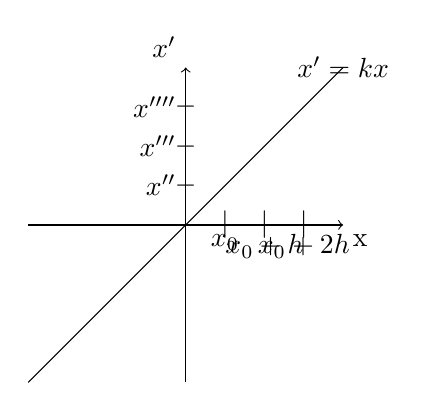
\begin{tikzpicture}[scale=1] %[x={10.0pt},y={10.0pt}]
	\pgfmathsetmacro\MAX{2}
	\draw[->] (-\MAX,0) -- (\MAX,0) node[anchor=north west] {x};
	\draw[->] (0,-\MAX) -- (0,\MAX) node[anchor=south east] {$ x'$};
	\draw[domain=-2:2,smooth,variable=\x] plot ({\x},{\x}) node {$ x'=kx$};
	\draw node at (0.5,0) {$|$};
	\draw node at (1,0) {$|$};
	\draw node at (1.5,0) {$|$};
	\draw node at (0,0.5) {$-$};
	\draw node at (0,1) {$-$};
	\draw node at (0,1.5) {$-$};
	\draw node[anchor=north] at (0.5,0) {$x_0$};
	\draw node[anchor=north] at (1,0) {$x_0+h$};
	\draw node[anchor=north] at (1.5,0) {$x_0+2h$};
	\draw node[anchor=east] at (0,0.5) {$ x'' $};
	\draw node[anchor=east] at (0,1) {$ x''' $};
	\draw node[anchor=east] at (0,1.5) {$ x''''$};
	
	\end{tikzpicture}% pic 1
	\qquad % <----------------- SPACE BETWEEN PICTURES
	\begin{tikzpicture}[scale=1] %[x={10.0pt},y={10.0pt}]
	\pgfmathsetmacro\MAX{2}
	\draw[->] (-\MAX,0) -- (\MAX,0) node[anchor=north west] {t};
	\draw[->] (0,-\MAX) -- (0,\MAX) node[anchor=south east] {x};
	\end{tikzpicture}% pic 2
\end{center}

blablabla ....\\
.......\\
Limiti di questo modello:
\begin{itemize}
	\item la variabile $x$ dovrebbe variare in $\N$, poiché una popolazione ha un numero intero di elementi.
	\item In molte specie è verosimile che il numero di nati al tempo $t$ dipenda dalla popolazione presente ad un tempo precedente $x(t-T), T>0$
	\item Supporre che una popolazione abbia per sempre a disposizione risorse sufficienti può non essere realistico
	\item Questo modello va bene quando si considerano intervalli di tempo molto lunghi.
\end{itemize}

\section{Teoria Locale}
\begin{definition}
	Una funzione $f:I\times A\to \R^n$, con $I$ intervallo in $\R$ e $A$ aperto in $\R^n$, si dice \textbf{localmente lipshitziana} in $x\in A$ \textbf{uniformemente} rispetto a $t$ se
	$$\forall x_0 \in A, \exists r>0 e L>0: \forall x_1,x_2 \in (B(x_0,r)\cap A), \forall t\in I$$
	vale che
	$$\norm{f(t,x_2)-f(t,x_1)}\leq L\cdot\norm{x_2-x_1}\qquad o, ugualmente\qquad\frac{\norm{f(t,x_2)-f(t,x_1)}}{\norm{x_2-x_1}}\leq L$$
	La lipschitzianità (\textbf{lips.}), in parole povere, valuta il rapporto tra incremento della $f$ e delle $x$ è minore di un valore fisso $L$
\end{definition}
\begin{note}
	La località è data da $x_1,x_2 \in (B(x_0,r)\cap A)$ e l'uniformità da $\forall t\in I$. Quindi la $f$ rimane lips. in modo uniforme al variare di $t$ (cioè $\forall t\in I$), ma questo non è garantito $\forall x\in A$, solo per $x_1,x_2 \in (B(x_0,r)\cap A)$.
\end{note}
\begin{note}
	\hypertarget{note:if_lips_then_loclips}
	Se $f$ \textbf{lips} su $A\implies f$ \textbf{loc. lips.} su A
\end{note}
\begin{example}
	La funzione $f:\R\mapsto\R$ data da $f(x)=x^2$ è \textbf{loc. lips.} su $\R$ ma non è \textbf{globalmente lips.} su $\R$. Vedasi \ref{def:fun_lips}
\end{example}
\begin{proposition}
	Siano $I\subseteq \R$ un intervallo aperto ed $A\subseteq \R^n$ un aperto. Ogni funzione $f\in \cntclass{1}(I\times A,R^n)$ è loc. lips in $x\in A$ uniformemente rispetto a $t\in I$.
	\begin{proof}
		sia $x\in A \Rightarrow \exists B(x_0,r)\subseteq A$ (per definizione di 
		\hyperref[def:aperto]{aperto}) con $r>0$, anche $\overline{B(x_0,r)}\subseteq A$ scelto $r$ abbastanza piccolo, allora $\norm{f(t,x_2)-f(t,x_1)}\le\sup\limits_{(t,x)\in I\times \overline{B(x_0,r)}}\norm{Df()}\norm{x_2-x_1}  $ per la formula degli \hyperref[thm:accresc_fin]{accrescimenti finiti}.
		% TODO da rivedere
	\end{proof}
\end{proposition}

\subsection{Esistenza e Unicità}
\begin{proposition}[Teorema di Peano]
	\label{teo:peano}
	Si consideri il seguente problema di Cauchy:
	$$\left\{\begin{matrix} x'=f(t,x)\\x(t_0)=x_0\end{matrix}\right.$$
	con $f:I\times A\in \R^n$ soddisfacente alle ipotesi:
	\begin{enumerate}
		\item $t_0\in \circdot{I}, x_0\in \circdot{A}$
		\item $f\in \cntclass{0}(I\times A;R^n)$
	\end{enumerate}
	inoltre $I\subseteq \R$ intervallo e $A\subseteq \R^n$, in quanto \hyperref[def:prob_cauchy_ord_1]{problema di Cauchy}.\\
	Allora esiste un $\delta>0$ tale che esiste soluzione $x:J\mapsto A$ del problema di Cauchy con $J=\realintervalclose{t_0-\delta}{t_0+\delta}$.
	\begin{note}
		$\delta$ è un valore arbitrario che serve ad identificare l'intervallo $I$ a cui appartiene $t_0$
	\end{note}
	\noindent Inoltre:
	\begin{itemize}
		\item $J\subseteq I$ da \hyperref{note:diff_eq_sol_definition_set}{nota definizione 47}, dunque $\varphi(J)\subseteq A$
		\item $\varphi(t_0)=x_0$
		\item $\varphi$ derivabile e $\varphi'(t)=f(t,\varphi(t))$
	\end{itemize}
	\begin{proof}
		Non richiesta
	\end{proof}
\end{proposition}
\begin{example}[Il Baffo/Pennello di Peano] % TODO da rivedere
	$$\left\{\begin{matrix} x'=\sqrt{\abs{x}}\\x(0)=x_0\end{matrix}\right.$$
	\begin{center}
		\begin{tikzpicture}[scale=1] %[x={10.0pt},y={10.0pt}]
		\pgfmathsetmacro\MAX{2}
		\draw[->] (-\MAX,0) -- (\MAX,0) node[anchor=north west] {x};
		\draw[->] (0,-\MAX) -- (0,\MAX) node[anchor=south east] {$ x'$};
		\draw[domain=0:2,smooth,variable=\x] plot ({\x},{(\x)^(1/2)});
		\draw[domain=-2:0,smooth,variable=\x] plot ({\x},{(-\x)^(1/2)});
		%\draw node at (0.5,0) {$|$};
		%\draw node at (1,0) {$|$};
		%\draw node at (1.5,0) {$|$};
		%\draw node at (0,0.5) {$-$};
		%\draw node at (0,1) {$-$};
		%\draw node at (0,1.5) {$-$};
		%\draw node[anchor=north] at (0.5,0) {$x_0$};
		%\draw node[anchor=north] at (1,0) {$x_0+h$};
		%\draw node[anchor=north] at (1.5,0) {$x_0+2h$};
		%\draw node[anchor=east] at (0,0.5) {$ x'' $};
		%\draw node[anchor=east] at (0,1) {$ x''' $};
		%\draw node[anchor=east] at (0,1.5) {$ x''''$};
		
		\end{tikzpicture}% pic 1
		\qquad % <----------------- SPACE BETWEEN PICTURES
		\begin{tikzpicture}[scale=1] %[x={10.0pt},y={10.0pt}]
		\pgfmathsetmacro\MAX{2}
		\draw[->] (-\MAX,0) -- (\MAX,0) node[anchor=north west] {t};
		\draw[->] (0,-\MAX) -- (0,\MAX) node[anchor=south east] {x};
		\end{tikzpicture}% pic 2
	\end{center}
	Se $x_0 = 0$ ho che $\varphi(t)=0$ è soluzione $\forall t$\\
	Ma $x' = \sqrt{\abs{x}}$ è anche un'equazione a variabili separabili, quindi risolvibile.
	$$\frac{x}{\sqrt{\abs{x}}}=1 \Rightarrow \int_{0}^{t}{\frac{ x'}{\sqrt{\abs{x}}}\integrald{t}} = t$$
	$$\int_{x(0)=0}^{x(t)}{\frac{1}{\sqrt{\abs{x}}}\integrald{x}} = t$$
	valuto ora il caso $x\geq0$, quindi $\abs{x}=x$
	$$\int_{x(0)=0}^{x(t)}{\frac{1}{\sqrt{x}}\integrald{x}} = 2\sqrt{x} = t$$
	La soluzione cercata è quindi $x(t)=\frac{1}{4}t^2$, estendendo il ragionamento ai tempi negativi si trova che la soluzione cercata è: $$\varphi(x)= \left\{\begin{matrix}+\frac{1}{4}t^2&&t>0,\\0&&t=0\\-\frac{1}{4}t^2&&t<0\end{matrix}\right.$$
	Abbiamo trovato che per la condizione iniziale $x_0=0$ il sistema ammette due soluzioni, si riesce estendere la soluzione a infinite funzioni.
	$$\varphi(x)= \left\{\begin{matrix}-\frac{1}{4}(t-a)^2&&t<a,\\0&&t\in[a,b]\\+\frac{1}{4}(t-b)^2&&t>b\end{matrix}\right.$$
	infatti:
	$$\varphi'(t) = \left\{\begin{matrix}-\frac{1}{8}(t-a)&&t<a,\\0&&t\in[a,b]\\+\frac{1}{8}(t-b)&&t>b\end{matrix}\right.$$ $$\left\{\begin{matrix}-\frac{1}{8}(t-a)=\frac{-\frac{1}{4}(t-a)^2}{	\sqrt{-\frac{1}{4}(t-a)^2}}&&t<a,\\0=0&&t\in[a,b]\\+\frac{1}{8}(t-b)=\frac{\frac{1}{4}(t-b)^2}{\sqrt{\frac{1}{4}(t-b)^2}}&&t>b\end{matrix}\right. = ....????? sistema $$
	Abbiamo quindi trovato infinite soluzioni.\\
	Questo esempio per sottolineare che il teorema di Peano non garantisce l'unicità della soluzione
\end{example}
\begin{example}[Continuità ed ipotesi necessaria] % TODO da rivedere
	Questo esempio mostra che se non c'è continuità, può?????????? non esserci la soluzione.\\
	Dato il seguente problema di Cauchy: $\left\{\begin{matrix}
	x' = \left\{\begin{matrix}1&&x<0\\-1&&x\ge 0\end{matrix}\right.\\
	x(0)=0
	\end{matrix}\right.$\\
	\begin{center}
		\begin{tikzpicture}[scale=1] %[x={10.0pt},y={10.0pt}]
		\pgfmathsetmacro\MAX{2}
		\draw[->] (-\MAX,0) -- (\MAX,0) node[anchor=north west] {x};
		\draw[->] (0,-\MAX) -- (0,\MAX) node[anchor=south east] {$ x'$};
		\draw[domain=0:2,smooth,variable=\x] plot ({\x},{1});
		\draw[domain=-2:0,smooth,variable=\x] plot ({\x},{-1});
		\draw node at (0,-1) {$\bullet$};
		\draw node at (0,1) {$\circ$};
		\end{tikzpicture}% pic 1
	\end{center}

	\noindent $x(t)=0$ soddisfa la condizione iniziale ma ovviamente non può essere soluzione del problema poiché per $x\ne 0$ si ha che $ x'=\pm 1$ che non è la derivata della funzione nulla.\\
	partendo sempre dalla condizione iniziale si può ipotizzare per esempio che la soluzione cresca, solo che questo contraddice $ x'(0)=-1$\\
	se invece si ipotizza che decresce da $0$ si ottiene che la funzione assume valori negativi, anche questo è un assurdo poiché la derivata per valori negativi della funzione è positiva.\\
	Precisiamo che se il problema fosse stato $\left\{\begin{matrix}
	x' = \left\{\begin{matrix}1&&x<0\\-1&&x\ge 0\end{matrix}\right.\\
	x(0)=-3\end{matrix}\right.$ allora la funzione $\varphi(x)=-x+3$ sarebbe stata soluzione nell'intervallo $J=\left] -\infty,0 \right[ $
\end{example}

\begin{theorem}[Teorema di Cauchy Locale]
	\label{teo:cau_locale}
	In sostanza si dimostra che il problema di Cauchy è ben posto nel senso di Hadamard.\\
	Si consideri il problema di Cauchy:
	$$\begin{cases}x'=f(t,x)\\x(t_0)=x_0\end{cases}$$
	con $f:I\times A \to \R^n$ soddisfacente le ipotesi:
	\begin{enumerate}
		\item $t_0\in \circdot{I}, x_0\in \circdot{A}$. Inoltre da \ref{def:equaz_diff} e note successive: $I$ intervallo e $I\subseteq \R^n$, inoltre $A\subseteq \R^n$
		\item $f\in \cntclass{0}(I\times A; \R^n)$ 
		\item $f$ è localmente Lipschitziana in $x\in A$ uniformemente rispetto a $t\in I$
	\end{enumerate}
	\begin{note}
		Le prime due ipotesi garantiscono l'esistenza, grazie al Thm. di Peano. La terza ipotesi rende il teorema più restrittivo, ma permette anche di giungere ad una conclusione più forte (ed utile).
	\end{note}
	Allora ho i seguenti risultati:
	\begin{enumerate}
		\item \textbf{Esistenza} (da \ref{teo:peano}): $\exists \delta>0$ con cui si identifica un $J=\realintervalclose{t_0-\delta}{t_0+\delta}$, inoltre $\exists\,\varphi : J \to \R^n$ soluzione con le proprietà date da Peano:
		\begin{itemize}
			\item $J\subseteq I$ da \hyperref{note:diff_eq_sol_definition_set}{nota definizione 47}, dunque $\varphi(J)\subseteq A$
			\item $\varphi(t_0)=x_0$
			\item $\varphi$ derivabile e $\varphi'(t)=f(t,\varphi(t))$
		\end{itemize}
		\item \textbf{Unicità}\\
		Se $\exists\,J_1,J_2$ intervalli con $J_1\subseteq I,J_2\subseteq I$ e $\exists\,\varphi_1:J_1\to \R^n, \varphi_2:J_2\to \R^n$ soluzioni con le seguenti proprietà
		\begin{itemize}
			\item $J_1\subseteq I$, $J_2\subseteq I$ da \hyperref{note:diff_eq_sol_definition_set}{nota definizione 47}, dunque $\varphi_1(J_1)\subseteq A$ e $\varphi_2(J_2)\subseteq A$
			\item $\varphi_1(t_0)=x_0,\,\varphi_2(t_0)=x_0$
			\item $\varphi_1,\varphi_2$ derivabili e
				$\begin{cases}
					\varphi_1'(t)=f(t,\varphi_1(t))\,\forall t \in J_1\\
					\varphi_2'(t)=f(t,\varphi_2(t))\,\forall t \in J_2
				\end{cases}$
				NB. Non è effettivamente sistema
		\end{itemize}
		\begin{note}
			Si può osservare che, sicuramente, $J_1\cap J_2\neq\emptyset$, poiché entrambi gli insiemi contengono almeno $t_0$ nella loro parte interna.		
		\end{note}
		Allora $\varphi_1(t)=\varphi_2(t)$ $\forall t \in(J_1\cap J_2)$\\
		Cioè, se esistono due soluzioni, allora esse coincidono ovunque siano entrambe definite.
		\item \textbf{Dipendenza Continua Dai Dati}\\
		Si considerino i seguenti problemi di Cauchy con condizione iniziale individuata nello stesso istante:
		$$(1)\begin{cases}x'=f(t,x)\\x(t_0)=x_0\end{cases}\qquad
		(2)\begin{cases}y'=g(t,y)\\y(t_0)=y_0\end{cases}$$
		con $f,g:I\times A \to \R^n$ e soddisfacenti le ipotesi di questo teorema.\\
		Allora esiste un $\delta >0$ tale che sull'intervallo $\realintervalclose{t_0-\delta}{t_0+\delta}$ sono definite una soluzione $\varphi$ di (1) ed una soluzione $\psi$ di (2). Inoltre esiste $L>0$ t.c. $\forall t\in \realintervalclose{t_0-\delta}{t_0+\delta}$ vale:
		$$\norm{\varphi(t)-\psi(t)} \le (\norm{x_0-y_0}+\delta\norm{f-g}_{\cntclass{0}})e^{L\abs{t-t_0}}$$
		dove $\norm{f-g}_{\cntclass{0}}=\sup\limits_{I\times A}\norm{f(t,x)-g(t,x)}$
	\end{enumerate}
\end{theorem}
\begin{note}
	Si ricorda la nota \hyperlink{note:if_lips_then_loclips}{alla definizione di locale lipschitzianità}
\end{note}
\observation
L'equazione integrale 
$$x(t)=x_0+\int_{t_0}^{t}f(\tau,x(\tau))\integrald{\tau}$$
viene spesso denominata EQUAZIONE DI VOLTERRA.\\
Questa equazione ha senso anche per alcune funzioni $f$ non non continue ma solo misurabili nel primo argomento. Ne consegue che nei Teoremi di esistenza ed unicità (locali/globali) l'ipotesi "$f$ continua" può essere sostituita da "$f$ continua tratti in $t, \forall x$, continua in $x$ e limitata"
\observation
la norma dell'integrale è minore uguale dell'integrale della norma.
\proposition LEMMA DI GRONWALL\\
Dati $a,b\in \R$ con $a\le b$ siano $\delta_0\in \left[ 0;+\infty \right]$ e $\delta,\kappa:\left[a,b\right]\to \R$ funzioni continue su $\left[a,b\right]$ con $\delta(t)\ge 0$,$\kappa(t)\ge 0 \quad \forall t\in\left[ a,b\right] $ e $\delta(t)\le \delta_0+\int_{a}^{t}\kappa(\tau)\delta(\tau)\integrald{\tau}$Allora $$\delta(t)\le\delta_0e^{\int_{a}^{t}\kappa(\tau)\integrald{\tau}}$$
Questo teorema porta da una stima implicita di $\delta$(sotto il segno di integrale) ad una stima esplicita 
\begin{proof}
	sia $\delta_0 > 0$. Sia $\Delta(t)=\delta_0+\int_{a}^{t}\kappa(\tau)\delta(\tau)\integrald{\tau}$.\\
	Vale per ipotesi che $\delta(t)\le\Delta(t)=\delta_0+\int_{a}^{t}\kappa(\tau)\delta(\tau)\integrald{\tau}$\\
	Sfruttando la derivata di $ln(\Delta(t))$ si ottiene $\frac{d}{\integrald{t}}(ln(\Delta(t)))= \frac{\Delta'(t)}{\Delta(t)}=\frac{\kappa(t)\delta(t)}{\Delta(t)}$, ed il termine $\frac{\delta(t)}{\Delta(t)}\le 1$, Integrando il primo e l'ultimo termine
	$$\int_{a}^{t}\left( \frac{d}{\integrald{t}}\left(ln(\Delta(t))\right) \right)\le\int_{a}^{t}\kappa(\tau)\integrald{\tau}$$
	$$ln(\Delta(t))\le ln(\delta_0)+\int_{a}^{t}\kappa(\tau)\integrald{\tau}$$
	$$ \Delta(t)\le\delta_0e^{\int_{a}^{t}\kappa(\tau)\integrald{\tau}} $$
	Da cui la tesi.
	Se $\delta_0=0$, ponendo $\Delta(t)=\epsilon+\int_{a}^{t}\kappa(\tau)\delta(\tau)\integrald{\tau}$ si ottiene $\delta(t)\epsilon$ ................... e il mio cervello sta bruciando
\end{proof}

\begin{proof}
	Cauchy Locale:\\
	L'idea alla base della dimostrazione è che vogliamo riuscire a trasformare il problema di Cauchy in un problema di punto fisso.Prima di tutto serve una relazione che dal problema di Cauchy ci permetta di ottenere $x$ in funzione di qualcosa che dipenda da $x$.\\
	Integrando ambi i membri della prima equazione del problema di ottiene:
	$$\int_{t_0}^{t}( x')\integrald{\tau}=\int_{t_0}^{t}(f(\tau,x(\tau)))\integrald{\tau}$$
	$$x(t)=x_0+\int_{t_0}^{t}(f(\tau,x(\tau)))\integrald{\tau}$$
	$T$ è una funzione del tipo:
	$\begin{array}{rcl} T: ? & \to & ? \\ x & \to & Tx \end{array}$, con $y(t)=x_0+\int_{t_0}^{t}(f(\tau,x(\tau)))\integrald{\tau}$\\
	Abbiamo raggiunto un problema di punto fisso ($x=Tx$). Ora bisogna determinare l'insieme di partenza e l'insieme di arrivo in maniera utile per la dimostrazione. Per poter applicare il Teorema delle contrazioni serve che lo spazio di partenza e di arrivo siano uguali e chiamiamo $\mathcal{X}$.\\
	$\begin{array}{rcl} T: \mathcal{X} & \to & \mathcal{X} \end{array}$ t.c.: $y(t)=(Tx)(t)=x_0+\int_{t_0}^{t}(f(\tau,x(\tau)))\integrald{\tau}$
	Bisogna quindi scegliere l'insieme $\mathcal{X}$. è un insieme di funzioni, in cui l'equivalenza sopra deve avere senso, cioè serve $x$ continua per avere l'equivalenza con il problema di Cauchy, quindi $\mathcal{X}=\cntclass{0}(\ldots)$.\\
	Inoltre volendo una soluzione del problema di Cauchy, la funzione $x(penso sia y(t)=x)$ deve essere definita almeno su un intervallo contenente $t_0$ nella sua parte interna, non interessa l'estensione di tale intervallo quindi si può scegliere $\left[t_0-\delta,t_0+\delta\right]$, inoltre deve avere valori in un insieme con $x_0$ nella sua parte interna, $\overline{B(x_0,r)}$. Quindi $\mathcal{X}=\cntclass{0}(\left[t_0-\delta,t_0+\delta\right];\overline{B(x_0,r)})$\\
	Per $\delta, r$ abbastanza piccoli si ha $\left[t_0-\delta,t_0+\delta\right]\subseteq I$, $\overline{B(x_0,r)}\subseteq A$, quindi adesso il problema è quello di determinare $\delta, r$.\\
	Per poter applicare il teorema delle contrazioni:
	\begin{description}
		\item[a-] $Tx$ definita (possibilità di calcolarla)
		\item[b-] $Tx\in\mathcal{X}$ (insiemi di partenza e arrivo)
		\item[c-] $Tx$ contrazione
		\item[d-] $\mathcal{X}$ completo
	\end{description}
	Se tutti questi punti sono soddisfatti, si può trovare $x=Tx$, cioè una $x$ che soddisfa l'equazione integrale e di conseguenza, per equivalenza, soluzione del problema di Cauchy.  
	\begin{description}
		\item[a-] $Tx$ definita significa poter calcolare l'integrale,per poter calcolare l'integrale devo poter calcolare la $f$, per calcolare la $f$ ho bisogno che $\tau$ e $x(\tau)$ stiano dentro gli insiemi su cui è definita la $f$, cioè $I,A$, per essere sicuri di non uscire dall'intervallo:
		$$\delta>0\quad t.c:\quad \left[t_0-\delta,t_0+\delta\right]\subseteq I$$
		OSS:: Se si cambiano $\delta, r$ con valori minori tutto vale ancora.\\
		OSS:: Per il problema x derivabile -> integrale  ... mi sosto in $\cntclass{0}$
		\item[b-] $Tx$ deve appartenere a $\mathcal{X}$. L'insieme $\mathcal{X}$ sostanzialmente pone tre vincoli a $Tx$: deve essere $\cntclass{0}$, definita in $\left[t_o-\delta;t_0+\delta\right]$ a valori in $\overline{B(x_0,r)}$.\\
		Per iniziare si verifica che sia definita in $\left[t_o-\delta;t_0+\delta\right]$\\
		.... qualcosa che non comprendo.... $\cntclass{0}$\\
		Resta da verificare che $Tx$ è a valori nella sfera, cioè che 
		$$(Tx)(t) \in \overline{B(x_0,r)}$$
		Valuto la distanza tra $(Tx)(t)$ e $x_0$. La differenza tra la posizione al tempo $t$ e al tempo $t_0$, questa distanza può essere controllata con la velocità e il tempo per cui il punto si è mosso.\\
		Chiamata $V$ la massima velocità alla quale può muoversi il punto, $V=\sup\limits{(t_0\times X_0)\in (\left[to+\delta,t_0-\delta\right]\times\overline{B(x_0,r)})}=\left\{\norm{f(t,x(t))}\right\}$ che è il sup della norma di f, cioè dei moduli dei vettori velocità, questo esiste sempre finito, non $\infty$ poiché $f$ è continua, la norma è continua , $t$ varia in un chiuso e limitato, $x_0$ varia in un chiuso e limitato, quindi stiamo calcolando  il sup di una funzione continua su un chiuso e limitato allora per il teorema di Weierstrass $V=\max\limits{(t_0\times X_0)\in (\left[to+\delta,t_0-\delta\right]\times\overline{B(x_0,r)})}=\left\{\norm{f(t,x(t))}\right\}$\\
		Non potendo modificare $V, \delta$ poniamo una restrizione su $r$:$V\delta < r$, da cui $\delta < r\cdot V$
		
		$$\norm{(Tx)(t) - x_0} = \norm{\int_{t_0}^t(f(\tau,x(\tau)))\integrald{\tau}} \le \abs{\int_{t_0}^t \norm{f(\tau,x(\tau))}\integrald{\tau}}\le$$
		$$\le\abs{\int_{t_0}^t V\cdot \integrald{\tau}}=V\abs{t-t_0}\le V\delta<r$$
		....aggiunto il modulo per $t<t_0$ e $t>t_0$ non lo si sa a priori\\
		quindi $\norm{(Tx)(t) - x_0}$ è minore di $r$ scelto $\delta$ opportunamente piccolo. 
		\item[c-] Se $Tx$ è una contrazione deve valere che
		$$\norm{Tx_2 - Tx_1}_{\cntclass{0}}\le K\norm{x_2-x_1}_{\cntclass{0}}\quad k\in\left[0,1\right[\quad\forall t\in\left[t_0-\delta,t_0+\delta\right]$$
		con $\norm{Tx_2-Tx_1}_{c^0}=\sup\limits_{t\in\left[t_0-\delta,t_0+\delta\right]}\norm{(Tx_2)(t) - (Tx_1)(t)}$, partendo da questa utilizzando prima la definizione di $f$ poi la linearità dell'integrale ....lipsh f... proprietà
		$$\norm{(Tx_2)(t) - (Tx_1)(t)}=$$
		$$\norm{x_0+\int_{t_0}^t f(\tau,x_2(\tau)) \integrald{\tau} - \left(x_0+\int_{t_0}^t f(\tau,x_1(\tau)) \integrald{\tau}\right)}=$$
		$$\norm{\int_{t_0}^t f(\tau,x_2(\tau))-f(\tau,x_1(\tau)) \integrald{\tau}}\le$$
		$$\abs{\int_{t_0}^t \norm{f(\tau,x_2(\tau))-f(\tau,x_1(\tau))} \integrald{\tau}}\le$$
		$$\abs{\int_{t_0}^t L\norm{x_2(\tau)-x_1(\tau)} \integrald{\tau}}\le$$
		$$L\abs{\int_{t_0}^t \norm{x_2-x_1}_{\cntclass{0}(\left[t_0-\delta,t_0+\delta\right];R^n)} \integrald{\tau}}=$$
		$$L\cdot \norm{x_2-x_1}_{\cntclass{0}(\left[t_0-\delta,t_0+\delta\right];R^n)}\abs{t-t_0}\le$$
		$$L\delta\norm{x-x_0}_{\cntclass{0}(\left[t_0-\delta,t_0+\delta\right];R^n)}$$
		cioè $\forall t \in \left[t_0-\delta,t_0+\delta\right]$ vale che $\norm{(Tx_2)(t)-(Tx_1)(t)}\le L\delta\norm{x_1-x_2}_{\cntclass{0}(\left[t_0-\delta,t_0+\delta\right];R^n)}$ e poiché è vero $\forall t \Rightarrow $ passando all'estremo superiore
		$$ \norm{Tx_1 - Tx_2}_{\cntclass{0}(\left[t_0-\delta,t_0+\delta\right];R^n)}\le L\delta\norm{x_1-x_2}_{\cntclass{0}(\left[t_0-\delta,t_0+\delta\right];R^n)}$$
		A questo punto scelto $\delta$ t.c. $L\delta<1$ ad esempio $\delta=\frac{1}{2L}$ così ottengo che per $\delta$ opportuno $Tx$ è una contrazione.		
		\item[d-] Bisogna mostrare che $\mathcal{X}$ è completo.\\
		Supponiamo che $\mathcal{X}\subseteq \cntclass{0}(\left[t_0-\delta,t_0+\delta\right];R^n)$, questo insieme è completo rispetto alla metrica $d_\infty=d_{\cntclass{0}}$, allora se abbiamo una successione $x_n$ di Cauchy in $\mathcal{X}$ lo è anche su $\cntclass{0}(\left[t_0-\delta,t_0+\delta\right];R^n)$, allora $\exists x_\infty\in \cntclass{0}(\left[t_0-\delta,t_0+\delta\right];R^n)$ con $x_n\to x_\infty$ per $n\to\infty$, ma poiché $\forall t \in\left[t_0-\delta,to+\delta\right]$ $x_\infty(t)=\lim\limits_{n\to\infty}x_n(t)$ e visto che $\forall t,\forall n\quad \norm{x_n(t)-x_0}\le r$ anche al limite vale $\norm{x_{\infty}(t)-x_0}\le r \Rightarrow x_\infty\in\mathcal{X}$ cioè $\mathcal{X}$ è completo.
	\end{description}
	Possimao a questo punto applicare il teorema delle Contrazioni allora $T$ ha un unico punto fisso allora l'equazione integrale ha un unica soluzione allora esiste la soluzione del problema di Cauchy e su $\left[t_0-\delta,t_0+\delta\right]$ possiamo gia dire che la soluzione  è unica.\\
	MA QUANTO CAZZO è LUNGA FORSE SONO A METà\\
	\begin{center}
		\begin{tikzpicture}[scale=2]
		\draw[->] (-0.5,0) -- (2,0) node[anchor=north west] {$t$};
		\draw[->] (0,-0.5) -- (0,2) node[anchor=south east] {$x$};
		%\draw[domain=0:2,smooth,variable=\x] plot ({\x},{1});
		%\draw[domain=-2:0,smooth,variable=\x] plot ({\x},{-1});
		\draw node at (0.5,0) {$\bullet$};
		\draw node[anchor=north] at (0.5,0) {$t_0-\delta$};
		\draw node at (1,0) {$\bullet$};
		\draw node[anchor=north] at (1,0) {$t_0+\delta$};
		\draw node at (1.5,0) {$\bullet$};
		\draw node[anchor=north] at (1.5,0) {$t_0$};
		%\draw node at (0,1) {$\circ$};
		\end{tikzpicture}% pic 1
	\end{center}
	FINIRE DISEGNO......\\
	OSS:: Passando da (a-), (d-) abbiamo ristretto sempre più il range di valori che $\delta, r$ possono assumere, così che alla fine è rimasto un intervallo sul quale è applicabile il teorema delle Contrazioni.\\
	Abbiamo trovato un intervallo $\left[t_0-\delta,t_0+\delta\right]$ in cui la soluzione esiste. Adesso osserviamo cosa accade prima a destra e poi a sinistra dell'intervallo con un ragionamento analogo.\\
	Soluzioni che sono coincidenti(cioè unica) in un intervallo possono non esserlo al di fuori dello stesso. Cauchy locale ci assicura che questo non può succedere.\\
	Sia per assurdo $t_M$ l'ultimo istante fino a cui $\varphi_1,\varphi_2$ coincidono, cioè: $t_M = \sup \left\{t\in I:t\ge t_0, \varphi_1(\tau)=\varphi_2(\tau), \forall \tau \in \left[t_0,t\right[\right\}$.\\
	Cerchiamo di mostrare o che non c'è o che è alla fine dell'intervallo $I$.\\
	Se si considera il problema di Cauchy:
	$\left\{\begin{matrix} x'=f(t,x(t))\\x(t_M)=x_{t_M}\end{matrix}\right.$. Possiamo applicare quanto trovato per il punto uno della tesi, cioè esiste un intervallo contenente $t_M$ nella sua parte interna in cui la soluzione esiste ed è unica.\\
	OSS:: $t_M$ esiste sempre poiché è il $sup$ di un insieme non vuoto, inoltre $t_M\ge t_0+\delta$ è certamente $t_M\in \overline{I}$\\
	Possono verificarsi due casi, o $t_M$ è sul bordo di $I$ ed in questo caso la dimostrazione è finita poiché fino al bordo dell'intervallo le soluzioni coincidono.
	Oppure $T_M$ è nella parte interna dell'intervallo quindi $t_m\ne\sup I\Rightarrow t_M\in\circdot{I}$, e se è u n punto interno per l'intervallo allora è anche un punto di accumulazione per lo stesso, è quindi possibile calcolare $\lim\limits_{t\to t_M^{-}}\varphi_1(t)\quad\lim\limits_{t\to t_M^{-}}\varphi_2(t)$ ma entrambi i limiti devono essere uguali a $x_M$ poiché sia $\varphi_1,\varphi_2$ sono soluzioni al problema  di Cauchy e devono quindi soddisfare la condizione iniziale, anche perché fino a $t_M$ le due soluzioni coincidono e quindi il loro limite deve essere lo stesso.\\
	Riguardo $x_M$ si può dire che:
	\begin{enumerate}
		\item se $x_M = A\Rightarrow$ le soluzioni coincidono fino alla fine dell'insieme $A$.
		\item se $x_m\in\circdot{A}$ abbiamo esattamente le ipotesi del teorema di Cauchy locale, per quanto visto si ha necessariamente che:\\
		$\exists \delta_M>0,\exists \varphi_M:\left[t_M-\delta_M,t_0+\delta_M\right]\to \R^n$ che è soluzione del nuovo problema impostato, UNICA per quanto detto sull'intervallo.
	\end{enumerate} 
	Applicando il ragionamento fino a quando non si raggiungono i bordi di $I$ e di $A$ abbiamo dimostrato che se esistono più soluzioni allora queste coincidono dove sono definite entrambe.\\
	FATTO IL SECONDO PUNTO DEL TEOREMA.\\
	Dati
	$$(P_f):\left\{\begin{matrix} x'=f(t,x(t))\\x(t_0)=x_{0}\end{matrix}\right.\quad	(P_g):\left\{\begin{matrix} y'=f(g,y(t))\\y(t_0)=y_{0}\end{matrix}\right.$$
	Siano $\varphi$ soluzione di $P_f$, $\psi$ soluzione di $P_g$, bisogna stimare quanto queste due soluzioni di due problemi con la condizione iniziale allo stesso istante distano.
	$$\varphi:\left[t_0-\delta_f,t_0+\delta_f\right]\to \R^n$$
	$$\psi:\left[t_0-\delta_g,t_0+\delta_g\right]\to \R^n$$
	chiamo $\delta=\min{\delta_f,\delta_g}$ che sicuramente soddisfa entrambe. Per stimare la distanza tra le soluzioni valuto:
	$$
	\norm{\varphi(t)-\psi(t)}=
	\norm{ x_0+\int_{t_0}^t f(\tau,\varphi(\tau))\integrald{\tau} - y_0 - \int_{t_0}^t g(\tau,\psi(\tau))\integrald{\tau}}
	$$
	linearità integrale disuguaglianza norma... modulo per i differenziali ....\\
	$$ \norm{x_0-y_0}+\abs{\int_{t_0}^{t} \norm{f(\tau,\varphi(\tau))-g(\tau,\psi(\tau))}\integrald{\tau}}\le$$
	adesso all'interno dell'integrale aggiungo e tolgo la quantità $f(\tau,\psi(\tau))$ e applico la disuguaglianza triangolare riarrangiando i termini
	$$ \norm{x_0-y_0}+\abs{\int_{t_0}^{t} \norm{f(\tau,\varphi(\tau))-f(\tau,\psi(\tau))}+\norm{f(\tau,\psi(\tau))-g(\tau,\psi(\tau))}\integrald{\tau}}\le$$
	$$ \norm{x_0-y_0} + \norm{f-g}_{c^0}\abs{t-t_0} +\abs{\int_{t_0}^{t} L\norm{\varphi(\tau)-\psi(\tau)} \integrald{\tau}}$$
	per comodità restringiamo la trattazione al caso $t>t_0$ sparisce il modulo. Riscrivo il primo e l'ultimo membro della disuguaglianza
	$$ \norm{\varphi(t)-\psi(t)}\le  \left[ \norm{x_0-y_0} + \delta\norm{f-g}_{c^0}\right] +\abs{\int_{t_0}^{t} L\norm{\varphi(\tau)-\psi(\tau)} \integrald{\tau}}$$
	$$ \left( \delta(t)\le\delta_0+\int_{t_0}^t \kappa(\tau)\delta(\tau)\integrald{\tau} \right)::Gronwall$$
	$$ \norm{\varphi(t)-\psi(t)}\le\left[\norm{x_0-y_0}+\delta\norm{f-g}_{\cntclass{0}}\right]+e^{L\abs{t-t_0}}$$
	QUESTO TEOREMA è TROPPO DA PRO.
\end{proof}
ESEMPIO: DECADIMENTO RADIOATTIVO\\
Il decadimento di una sostanza radioattiva è ben descritto da $ x'=-k\cdot x$ dove $x$ è la quantità di sostanza radioattiva non ancora decaduta e $k$ è una costante propria di ogni singolo materiale\\
...........\\
ESEMPIO: LEGGE DEL CALORE DI NEWTON\\
......\\
ESEMPIO: CRESCITA LOGISTICA\\
......\\
\section{Teoria Globale}
\proposition
Siano $(X,d_x)$ e $(Y,d_y)$ spazi metrici, sia $f:A\subseteq X\to Y$. Se $f$ è uniformemente continua su $A$ allora $\exists ! \overline{f}:\overline{A}\to Y$ t.c. $\overline{f}_{\left|A\right.}=f$. cioè $f$ può essere estesa in modo unico alla chiusura dell'insieme $A$.
\definition
Una funzione $f:I\times \R^n\to \R^n$ con $I$ intervallo in $R$ si dice sub lineare se esistono due costanti positive $A$ e $B$ t.c.: $\forall t \in I$ 
$$ \norm{f(t,x)}\le A + B\norm{x}$$\\
ESEMPIO:: $f(t,x)=x^2$ NON SUBLINEARE\\
ESEMPIO:: $f(t,x)=sin(x^2)$ SUBLINEARE\\
\observation 
Sia $f(t,x)$ globalmente Lipshitziana in $x$ uniformemente in $t$ allora $f$ sublineare.
$$\exists L\ge 0 :\forall x_1,x_2\in \R^n, t\in I, \norm{f(t,0)}\le A$$
$$\norm{f(t,x_2)-f(t,x_1)}\le\norm{x_2-x_1}$$
$$\norm{f(t,x)}\le\norm{f(t,x_0)}+\norm{f(t,x)-f(t,0)}\le A +L\norm{x}$$
In sostanza una funzione è sublineare se esiste una retta tale per cui il grafico della funzione è tutto nella regione di piano delimitata da questa retta.
	\begin{center}
	\begin{tikzpicture}[scale=2]
	\draw[->] (-2,0) -- (2,0) node[anchor=north west] {$x$};
	\draw[->] (0,-2) -- (0,2) node[anchor=south east] {$y$};
	\draw[domain=-2:2,smooth,variable=\x] plot ({\x},{0.25*abs(\x)+0.5});
	\draw[domain=-2:2,smooth,variable=\x] plot ({\x},{-(0.25*abs(\x)+0.5)});
	\end{tikzpicture}% pic 1
\end{center}
ESEMPIO::$x\cdot sin(x)$ SUBLINEARE\\
ESEMPIO::$x^2\cdot sin(x)$ NO SUBLINEARE\\
ESEMPIO::$e^x$ NO SUBLINEARE\\
Diciamo sublineare se il grafico non si impenna.\\
\proposition
Data la funzione $f:I\times \R^n\to \R^n$, se:
\begin{enumerate}
	\item $I\subseteq \R$ è un intervallo, con $t_0\in\circdot{R^n}$
	\item $f\in \cntclass{0}(I\times \R^n;R^n)$
	\item $f$ è localmente Lipschitziana in $x\in \R^n$ uniformemente rispetto $t\in I$
	\item $f$ è sublineare
\end{enumerate}
allora il problema di Cauchy $\left\{\begin{matrix} x'=f(t,x)\\x(t_0)=x_0\end{matrix}\right.$ ammette un'unica soluzione definita sull'intervallo $I$.
\begin{proof}
	DISEGNO...\\
	Il teorema di Cauchy Locale assicura che  la soluzione esiste unica su un intervallo centrato all'istante iniziale.
	Bisogna dimostrare che la soluzione può essere estesa a tutto l'intervallo. Questo non si può fare in due casi:
	\begin{enumerate}
		\item c'è un asintoto verticale
		\item oscilla tanto che a un certo punto non va più avanti
	\end{enumerate}
	Quindi i casi in cui la soluzione non si può estendere su tutto l'intervallo sono quelli in cui non esiste il limite della soluzione. Quindi dobbiamo evitare tali comportamenti.\\
	Ragionamento da $t_0$ in avanti.\\
	Sia $T=sum\left\{t\in I :\exists soluzione su \left[ t_0,t \right[ \right\}$ cioè prendo l'estremo superiore dei tempi per cui c'è una soluzione.
	Se $T= sup I$ o $T=+\infty$ abbiamo la tesi.\\
	Se $T$ finito con $T<sup I$, dimostrando che la derivata della soluzione è limitata si escludono i casi in cui l'estensione della soluzione non si può fare.
	quindi bisogna mostrare $ x' = f(t,x)$ è limitata sull'insieme dove può arrivare la $x$\\
	Sia ora $\varphi$ soluzione del problema di Cauchy:
	$$ \varphi(t) = x_0 + \int_{t_0}^tf(\tau,x(\tau))\integrald{\tau}$$
	Valuto allora\\
	$\norm{\varphi(t)}\le \norm{x_0} + \abs{\int_{t_0}^tf(\tau,\varphi(\tau))\integrald{\tau}}=\norm{x_0} + \int_{t_0}^t\norm{f(\tau,\varphi(\tau))}\integrald{\tau}$ poiché $t\in\left[t_0,T\right[$\\
	$\norm{\varphi(t)}\le \norm{x_0} + \int_{t_0}^t\left(A+B\norm{\varphi(\tau)}\right)\integrald{\tau}$ poiché f è sublineare.\\
	$\norm{\varphi(t)}\le \norm{x_0} + A(T-t_0)+\int_{t_0}^t B\norm{\varphi(\tau)}\integrald{\tau}$\\
	...\\
	applico il Gronwall e risulta che
	$$\norm{\varphi(t)}\le\left(\norm{x_0}+A(t-t_0)\right)e^{B(t-t_0)}\le\left(\norm{x_0}+A(t-t_0)\right)e^{B(T-t_0)}$$	
	Abbiamo quindi dimostrato che la $f$ resta limitata.\\
	Posso guardare alla funzione come segue:\\
	$$
	\sup
	\left\{f(t,x): t\in\left[t_0,T\right[, x\in \overline{B\left(x_0,
		\left[ 
			\norm{x_0} A \left(T-t_0\right)
		\right]e^{B\left(T-t_0\right)}\right)}
	\right\}
	$$
	$\overline{B\left(x_0,
		\left[ 
		\norm{x_0} A \left(T-t_0\right)
		\right]e^{B\left(T-t_0\right)}\right)}
	$ è un insieme compatto poiché chiuso e limitato in $R^n$, $\varphi$ è limitata, la $f$ limitata, allora $ \varphi'$ limitata allora $\varphi$ lipshitziana allora $\varphi$ uniformemente continua.\\
		Allora esiste finito $\lim\limits_{t\to T^{-}}\varphi(t)=X$. Ora possono verificarsi due casi:\\
	\begin{enumerate}
		\item Se $T=\sup I \Rightarrow$ dimostrazione conclusa
		\item Se $T<\sup I \Rightarrow$ posso considerare il problema di Cauchy \\
		$\left\{ \begin{matrix}  x'=f(t,x)\\x(T)=X \end{matrix} \right.$ Questo è un assurdo poiché arriveremmo a trovare una soluzione definita oltre il tempo $T$. Questo nega la scelta fatta a inizio dimostrazione.
		\end{enumerate}
\end{proof}
\section{Equazioni Autonome}
\definition 
Un'equazione differenziale ordinaria in forma normale si dice autonoma sse la variabile indipendente (solitamente il tempo) non vi compare esplicitamente.
\observation
Tipicamente, le equazioni differenziali ordinarie autonome modellizzano sistemi isolati.
\observation Invarianza per traslazione temporale.\\
Non è importante ai fini dello studio dell'equazione l'istante iniziale, ma solo la lunghezza dell'intervallo.
Se  $x=\varphi(t)$ risolve $\left\{ \begin{matrix}  x' = f(x)\\x(t_0)=x_0 \end{matrix} \right.$\\
Allora $x=\varphi(t+t_0)$ risolve $\left\{ \begin{matrix}  x' = f(x)\\x(0)=x_0 \end{matrix} \right.$\\
\begin{proof}
	Sia $\psi(t)=\varphi(t_0+t)$\\
	$ \psi'(t)= \phi'(t_0+t)=f(\varphi(t_0+t))=f(\psi(t))$\\
	$\psi(0)=\varphi(t_0)=x_0$ 
\end{proof}
\proposition Teorema dell'energia cinetica\\
Un punto materiale non vincolato $P$ di massa $m$ si muove sotto l'azione di una forza $F$ che dipende solo dalla posizione di $P$. Allora la variazione di energia cinetica di $P$ è uguale al lavoro compiuto su $P$ da questa forza.
\begin{proof}
	sia $\underline{x}=(x,y,z)$ la terna delle coordinate di $P$. Per il Secondo Principio della Dinamica e per quanto assunto sulla forza $F$, il moto di $P$ è descritto dall'equazione(vettoriale) differenziale ordinaria del secondo ordine:\\
	$$m \underline{x''}=F(\underline{x})$$
	$$m \underline{x''}\cdot \underline{x'}=F(\underline{x}) \underline{x'}$$
	$$\frac{1}{2}m\frac{d}{\integrald{t}}\left(\left( \underline{x'}\right)^2\right)=F(\underline{x}) \underline{x'}$$
	$$\int_{0}^t\frac{1}{2}m\frac{d}{\integrald{t}}\left(\left( \underline{x'}(\tau)\right)^2\right)\integrald{\tau}=\int_{0}^tF(\underline{x}(\tau))\cdot \underline{x'(\tau)}\integrald{\tau}$$
	$$\frac{1}{2}m\left( x'(t)\right)^2-\frac{1}{2}m\left( x'(0)\right)^2 = \int_{x(0)}^{x(t)}F(\xi)d\xi$$
	L'ultimo integrale è calcolato lungo la traiettoria di $P$.
\end{proof}
ESEMPIO:: Il Lancio di un Paracadutista\\
.....\\
.....\\
.....\\
ESEMPIO:: CADUTA IN UN LIQUIDO\\
.....\\
.....\\
.....\\
\section{Equazioni Differenziali Ordinarie}
\definition
Sia $I\subseteq\mathbb{R}$ un intervallo e $n\in N$. Date le $n+1$ funzioni $a_0,a_1,\ldots,a_{n-1}, f:I\to\mathbb{C}$ si dice equazione differenziale ordinaria lineare di ordine $n$, l'equazione differenziale:
$$x^{(n)}+a_{n-1}(t)\cdot x^{(n-1)}+\ldots+a_1(t)\cdot x'+a_0(t)x=f(t)$$
Se $f\equiv 0 $ l'equazione si dice omogenea.
\proposition
sia $I$ un intervallo compatto e tale che $\circdot{I}\ne \emptyset$ siano $a_0,a_1,\ldots,a_{n-1},f\in \cntclass{0}(I;\mathbb{C})$. Allora $\forall t_0\in\circdot{I}$ e $c_0,c_1,\ldots,c_{n-1}\in\mathbb{C}$ il problema di Cauchy 
$$ \left\{\begin{matrix}[]
x^{(n)}=-\sum\limits_{k=1}^{n-1}\left(a_k(t)x^k\right)+f(t)\\
x(t_0)=c_0\\
x(t_2)=c_1\\
\ldots\\
x^{(n-1)}(t_0)=c_{n-1}\\
\end{matrix}\right.$$
ammette soluzione unica definita su tutto l'intervallo $I$.
\begin{proof}
	Un'equazione differenziale lineare di ordine $n$ può essere trasformato in un sistema di equazioni al primo ordine.
	Introduciamo la variabile $X\in\mathbb{\cntclass{n}}$ ed il dato iniziale $C\in\mathbb{\cntclass{n}}$
	$$\left[\begin{matrix} X_1\\X_2\\\ldots\\X_{n-1}\\X_n \end{matrix}\right] = \left[\begin{matrix} x\\ x'\\\ldots\\ x^{(n-1)}\\x^{(n)} \end{matrix}\right]\quad\quad\left[\begin{matrix} C_1\\C_2\\\ldots\\C_{n-1}\\C_{n} \end{matrix}\right] = \left[\begin{matrix} c_0\\c_1\\\ldots\\ c_{n-2}\\c_{n-1} \end{matrix}\right]$$
	il problema di Cauchy per l'equazione lineare diventa:
	$$
	\left\{
	\left[\begin{matrix} X_1'\\X_2'\\\ldots\\X_{n-1}'\\X_n' \end{matrix}\right]
	=
	\left[\begin{matrix} X_2\\X_3\\\ldots\\X_{n}\\-\sum\limits_{k=1}^{n-1}\left(a_k(t)x^k\right)+f(t) \end{matrix}\right]
	\\
	X(t_0)=C
	\right.
	$$
	La funzione
	$\begin{array}{rcl} 
	F: I\times\mathbb{C}^n & \to & \mathbb{C}^n \\
	   (t,X) & \to & \left[\begin{matrix} X_2\\X_3\\\ldots\\X_{n}\\-\sum\limits_{k=1}^{n-1}\left(a_k(t)x^k\right)+f(t) \end{matrix}\right] \\ 
	\end{array}$
	è lineare in $X$ e globalmente lipshitziana in $X$ uniformemente in $t$, infatti per ogni $X,Y\in\mathbb{C}^n$
	$$\norm{F(t,X)-F(t,Y)}\le \sqrt{1+\left( \max\limits_k \sup\limits_I \norm{a_k} \right)^2}\cdot\norm{X-Y}$$
	Sono soddisfatte le ipotesi di Cauchy Globale allora si ha la tesi.
\end{proof}
\observation
La locuzione lineare è giustificata dalla proposizione seguente.
\proposition
Sia $I\subseteq \R$ un intervallo e $n\in\mathbb{N}$. Date le $n+1$ funzioni $a_0,a_1,\ldots,a_{n-1},f:I\to\mathbb{C}$,l'operatore 
$\begin{array}{rcl} 
L: \cntclass{n}(I;\mathbb{C}) & \to & \cntclass{0}(I;\mathbb{C}) \\
x & \to & x^{(n)}+\sum\limits_{k=1}^{n-1}a_k(t)x^{(k)} \\ 
\end{array}$è lineare
\begin{proof}
	La linearità di $L$ equivale a:
	$$ \begin{matrix}L(x_1+x_2)=L(x_1)+L(x_2) && \forall x_1,x_2\in \cntclass{n}(I;\mathbb{C})\\L(\lambda\cdot x)=\lambda\cdot L(x) && \forall\lambda\in\mathbb{C}, \forall x\in \cntclass{n}(I;\mathbb{C})\end{matrix} $$
	Entrambe le condizioni  seguono dalle regole di derivazione.
\end{proof}
\section{Equazioni Lineari a Coefficienti Costanti}
\definition
Dati i coefficienti $a_0,a_1,\ldots,a_{n-1},b\in\mathbb{C}$, si dice equazione differenziale ordinaria lineare di ordine $n$ a coefficienti costanti l'equazione differenziale
$$x^{(n)}+a_{n-1}x^{(n-1)}+\ldots+a_1 x'+a_0x=b$$
se $b=0$ l'equazione si dice omogenea. La sua Equazione caratteristica è l'equazione algebrica
$$\lambda^n+a_{n-1}\lambda^{n+1}+\ldots+a_1\lambda+a_0=0$$ 
\observation
Nella risoluzione di equazioni differenziali lineari la funzione esponenziale $t\to e^{\lambda t}$ riveste un ruolo molto particolare. Questa funzione è un autovalore dell'operatore di derivazione $D$ relativo all'autovalore, risolve infatti $\lambda$:$Dx=\lambda\cdot x$ 
\proposition
Data l'equazione
$$x^{(n)}+a_{n-1}x^{(n-1)}+\ldots+a_1 x'+a_0x=b$$
$x(t)=e^{\lambda t}$ risolve l'equazione omogenea $\Leftrightarrow$ $\lambda$ è soluzione dell'equazione caratteristica.\\

LEMMA:: Sia $x(t)=t\cdot e^{\lambda\cdot t}$. Allora , per ogni $n\in\mathbb{N}, n\ge 1$
$$x^{(n)}(t)=\left(\lambda^nt+n\lambda^{n-1}\right)e^{\lambda t}$$
???????????????NON L?HO CAPITA BENE.......................\\
\proposition
Data l'equazione 
$$x^{(n)}+a_{n-1}x^{(n-1)}+\ldots+a_1 x'+a_0x=b$$
$x(t)=te^{\lambda t}$ risolve l'equazione omogenea $\Leftrightarrow$ $\lambda$ è soluzione dell'equazione caratteristica con molteplicità almeno ??????????.







\part{Calcolo delle Variazioni}
\part{Chapter}

\section{Preliminari}
Il calcolo delle variazioni si occupa dell'ottimizzazione di funzioni $\realfunction{F}{X}{\mathbb{R}}$, dove $X$ è un isieme di funzioni.\\
In questo capitolo varranno considerati univocamente funzionali integrali del tipo
$$\begin{array}{rcl} F: X & \to & \mathbb{R} \\
x & \to & \int_{a}^b f(t,x(t),\overset{\cdot}{x}(t))dt\end{array}$$
eventulmente soggetti a vincoli sui valori $x(a)$ e $x(b)$ o sul valore di un integrale del tipo $\int_a^b \varphi(x(t))dt$.\\
Dove:
$$\realfunction{f}{\realintervalclose{a}{b}\times\mathbb{R}^n\times\mathbb{R}^n}{\mathbb{R}}$$
$$X=\left\{x\in C^1(\realintervalclose{a}{b});\mathbb{R}^n\text{ t.c.: }x(a)=x_a, x(b)=x_b \right\},\text{ con }x_a,x_b\in\mathbb{R}^n$$
\proposition
Sia $f\in C^1(A\times\mathbb{R};\mathbb{R})$ con $a\subseteq\mathbb{R}^n$\\
Se $\begin{array}{ccc} F: \mathbb{R}\times\mathbb{R}\times A & \to & \mathbb{R} \\
x & \to & \int_{\alpha}^\beta f(x,t)dt\end{array}$
Allora:
$$ F\in C^1$$
$$ \partial_\alpha F(\alpha,\beta,x)=-f(x,\alpha)$$
$$ \partial_\beta F(\alpha,\beta,x)=f(x,\beta)$$
$$ \nabla_x F(\alpha,\beta,x)=\int_{\alpha}^{\beta}\nabla_xf(x,t)dt$$
\definition ?????????????? R OPPURE RN\\
Sia $I\in\mathbb{R}$ un intervallo. Curva su $I$ $\mathbb{R}\rightleftharpoons$ una funzione $\gamma:I\subseteq\mathbb{R}^n$ che sia continua.
\observation
$\gamma(I)$ si chiama supporto della curva,ed 1'e certamente connesso.(una funzione continua manda intervalli connessi in connessi)
\definition
Sia $\realfunction{\gamma}{\realintervalclose{a}{b}}{\mathbb{R}}^n$ una curva, lunghezza della curva $\rightleftharpoons l(\gamma)=\sup\left\{\sum\limits_{i=1}^{N}\left\|\gamma(t_i)-\gamma(t_{i-1})\right\|: N\in\mathbb{N}\,N>1,t_0=a,t_N=b,t_{i-1}<t_i, i=1,2,\ldots,N \right\}$ 
Cio\'e prendo una curvae la approssimo con una spezzata, la pi\'u lnga di tutte le poligonali è la lunghezza della curva.\\
DISEGNO\\
DISEGNO\\
\definition
Una curva $\realfunction{\gamma}{\realintervalclose{a}{b}}{\mathbb{R}^n}$ si dice rettificabile $\rightleftharpoons f(\gamma)<+\infty$
\observation
$$\sum\limits_{i=1}^{N}\left\| \gamma(t_i)-\gamma(t_{i-1}) \right\| $$
per il teorema del valore medio differenziale(accrescimenti finiti)
$$\sum\limits_{i=1}^{N}\left\| \overset{\cdot}{\gamma}(t_i)(t_i-t_{i-1})\right\| =??$$
$$\int_{a}^{b}\left\| \overset{\cdot}{\gamma}(t) \right\| dt$$
\proposition
Se $\gamma\in C^1(\realintervalclose{a}{b};\mathbb{R}^n)\Rightarrow l(\gamma)=\int_a^b\left\|\overset{\cdot}{\gamma}(t)\right\|dt$
\observation
Se $\gamma$ è la traiettoria di un punto materiale,allora $\left\|\gamma\right\|$ è la norma della elocit\'a istantanea, e quindi $l(\gamma)$ è lo spazio che si percorre, cio\'e l'integrale della velocit\'a valutato tra $t??????t_i$ due istanti di tempo entro i quali si mantiene tale velocit\'a.
\observation
Nel caso specifico sar\'a:
$$ X=\left\{ x\in C^1(\left[a,b\right];\mathbb{R}2): x(a)=A, x(b)=B \right\} $$
$$\begin{array}{ccc} 
F: X & \to & \mathbb{R} \\
x & \to & \int_{a}^b \left\|\overset{\cdot}{x}(t)\right\|dt
\end{array}$$
$$\begin{array}{ccc} 
f: \left[a,b\right]\times\mathbb{R}^2\times\mathbb{R}^2 & \to & \mathbb{R} \\
(t,x,\overset{\cdot}{x}) & \to &  \left\|\overset{\cdot}{x}(t)\right\|
\end{array}$$
\section{L'Equazione di Eulero}
LEMMA:::LEMMA FONDAMENTALE DEL CALCOLO DELLE VARIAZIONI\\
Sia $f\in C^0(\left[0,1\right];\mathbb{R})$ t.c.: $\forall v\in C^0(\left[0,1\right];\mathbb{R})$ con $v(0)=v(1)=0$ si abbia $\int_0^1 f(x)v(x)dx=0$\\
Allora $f(x)\equiv 0\forall x\in\left[0,1\right]$ 
\begin{proof}
	\begin{center}
		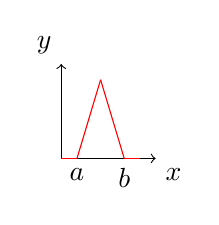
\begin{tikzpicture}[scale=1]
			\draw[->] (0,0) -- (1.2,0) node[anchor=north west] {$x$};
			\draw[->] (0,0) -- (0,1.2) node[anchor=south east] {$y$};
			\node[below] at (0.2,0) {$a$};
			\node[below] at (0.8,0) {$b$};
			\clip (0,0) rectangle (1,1);
			\draw[domain=0:0.2,smooth,red,variable=\x] plot ({\x},{0});
			\draw[domain=0.2:0.5,smooth,red,variable=\x] plot ({\x},{(1/0.3)*\x-(0.2/0.3)});
			\draw[domain=0.5:0.8,smooth,red,variable=\x] plot ({\x},{-(1/0.3)*\x+(0.8/0.3)});
			\draw[domain=0.8:1,smooth,red,variable=\x] plot ({\x},{0});
		\end{tikzpicture}
	\end{center}
	Per Assurdo, se $f\not\equiv 0$, allora $\exists\left[0,1\right]$ t.c. $f(x_0)\ne 0$.\\
	Osservo che se $x_0=0$ allora $\exists\overline{x}_0\in\left]0,1\right[$ t.c. $f(\overline{x}_0)\ne 0$.\\
	Osservo che se $x_0=1$ allora $\exists\overline{x}_0\in\left]0,1\right[$ t.c. $f(\overline{x}_0)\ne 0$\\
	Entrambe le osservazioni per la continuit\'a di $f$, significa che se $x_0$ è un punto in cui la $f>0$ allora per la continuit\'a della funzione anche li vicino si hanno valori maggiori di zero.\\
	Quindi si pu\'o pensare $x_0\in\left]0,1\right[$.\\
	Allora $\exists a,b\in\left]0,1\right[$ t.c. $x_0\in\left]a,b\right[ e \forall x\in\left]a,b\right[$ vale che $\left|f(x)\right|\ge\left|f(x_0)\right|$ sempre per la continuit\'a di $f$.\\
	Pensiamo $f(x_0)>0$ in questo modo $\left|f(x_0)\right|=f(x_0)$ e scegliamo la funzione $v(x)$ come disegnata: $v(x)=\left\{\begin{matrix}
	0&&x\le x_0-\delta\\
	\frac{x}{\delta}-\frac{x_0-\delta}{\delta}&& x_0-\delta<x<x_0\\
	1&& x=x_0\\
	-\frac{x}{\delta}+\frac{x_0+\delta}{\delta}&&x_0<x<x_0+\delta\\
	0&&x\ge x_0+\delta
	\end{matrix}\right.$POSSIBILIPLAUSIBILIERRORI\\
	Se calcoliamo
	$$\int_0^1f(x)v(x)dx=\int_a^bf(x)v(x)dx\ge\frac{1}{2}f(x_0)\int_a^bv(x)dx=\frac{1}{2}f(x_0)\frac{b-a}{2}>0$$
	Se avessi preso $f(x_0)<0$ prendo $v=-v$ e il resto segue...
\end{proof}
\observation
Questo lemma è concettualmente analogo al Teorema di Fermat nel capitolo delle derivate.
\corollary LEMMA CASO VETTORIALE.\\
Sia $f\in C^0(\left[a,b\right];\mathbb{R}^n)$ tale che $\forall v\in C^0(\left[a,b\right];\mathbb{R}^n)$ con $v(0)=v(1)=0$ si abbia $\int_0^1f(x)\bullet v(x)dx=0$ allora $f(x)\equiv 0$ $\forall x\in \left[0,1\right]$.
\begin{proof}
	Per questa dimostrazione si osservano componente per componente.\\
	$\forall i=1,2,\ldots,n$ scelgo $v_j(x)=\left\{\begin{matrix}0&&j\ne i\\v_i(x)&&j=i \end{matrix}\right.$\\
	A questo punto applico il lemma fondamentale alla componente $i$-esima $f_i$ di $f$.
\end{proof}
\corollary
Sia $f\in C^0(\left[a,b\right];\mathbb{R})$ e $k\in\mathbb{N}$ tale che $\forall v\in C^k(\left[a,b\right];\mathbb{R}^n)$ con $v(0)=v(1)=0$ si abbia $\int_0^1f(x)v(x)dx=0$ allora $f(x)\equiv 0$ $\forall x\in \left[0,1\right]$.
\begin{proof}
	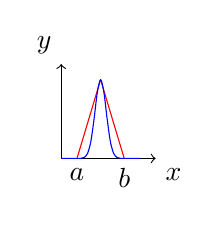
\begin{tikzpicture}[scale=1]
		\draw[->] (0,0) -- (1.2,0) node[anchor=north west] {$x$};
		\draw[->] (0,0) -- (0,1.2) node[anchor=south east] {$y$};
		\node[below] at (0.2,0) {$a$};
		\node[below] at (0.8,0) {$b$};
		\clip (0,0) rectangle (1,1);
		\draw[domain=0:0.2,smooth,red,variable=\x] plot ({\x},{0});
		\draw[domain=0.2:0.5,smooth,red,variable=\x] plot ({\x},{(1/0.3)*\x-(0.2/0.3)});
		\draw[domain=0.5:0.8,smooth,red,variable=\x] plot ({\x},{-(1/0.3)*\x+(0.8/0.3)});
		\draw[domain=0.8:1,smooth,red,variable=\x] plot ({\x},{0});
		\draw[domain=0:1,smooth,blue,variable=\x] plot ({\x},{ e^(-((\x-0.5)*10)^2) });
	\end{tikzpicture}
	\'E sempre lo stesso lemma con l'aggiunta che la funzione $v$ sia di classe $C^k$.\\
	Se si chiama $u$ la funzione blu e $v$ la funzione rossa abbiamo:
	$$\int_0^1 f(x)u(x)dx>0$$
	Se $v$ è un po pi\'u regolare , prendiamo $v=u^(k+1)(x)$. Cio\'e se vogliamo $v\in C^k$ prendiamo.....\\
	LA DINMOSTRAZIONE E A ME INCOMPRENSIBILE.
\end{proof}

\theorem EQUAZIONE DI EULERO.\\
Sia $f\in C^2\left(\left[a,b\right]\times\mathbb{R}^n\times\mathbb{R}^n;\mathbb{R}\right)$ con $a,b\in\mathbb{R}$ e $a<b$.\\
Sia $X=\left\{x\in C^2\left(\left[a,b\right];\mathbb{R}^n\right): x(a)=A, x(b)=B\right\}$ con $A,B\in\mathbb{R}^n$.\\
Sia $\begin{array}{ccc} F: X & \to & \mathbb{R} \\
x & \to & \int_{a}^b f(t,x(t),\overset{\cdot}{x}(t))dt\end{array}$.\\
Se la funzione $x_\ast\in X$ è t.c. $F(x_\ast)=\max\left\{F(x):x\in X \right\}$ [o min]\\
Allora $\partial_xf(t,x_\ast(t),\overset{\cdot}{x_\ast}(t))-\frac{d}{dt}\partial_{\overset{\cdot}{x}}f(t,x_\ast(t),\overset{\cdot}{x_\ast}(t))=0$.\\
Questa ultima equzione è l'equazione di Eulero-Lagrange del Funzionale $F$ o a volte detta variazione prima del funzionale $F$. è un sistema di $n$ equazioni differenziali ordinarie del secondo ordine nella funzione incognita $x_\ast$.
\begin{proof}
	 Sia $\varphi(h)=F(x_\ast+hv)$, dove $x_\ast\in X$ e $x_\ast+hv\in X$, con $h$ piccolo.\\
	 L'equazione di Eulero-Lagrange in apparenza complicata è analoga ad un equazione di analisi1 del tipo $f^{'}=0$ oppure in analisi due a $\nabla f=0$. solo che ora sono cavoli amari.\\
	 Come si sceglie la variazione $v$ in modo che $x_\ast+hv\in X$, con $h$ piccolo.\\
	 $X$ è l'insieme delle funzioni di $C^2$, si sa che $x_\ast\in C^2$, una scelta opportuna di $v$ è $v\in C^2(\left]a,b\right[;\mathbb{R}^n)$.\\
	 Inotre deve essere che $ x_\ast(a)+hv(a)=A$ e  $x_\ast(b)+hv(b)=B$ per restare dentro l'insieme $X$.
	 Quindi $v(a)=v(b)=0$.
	 $h$ è uno scalare e per ipotesi si sa che $F(x_\ast)$ è punto di massimo, quindi si conclude che $h=0$ è punto di massimo per la funzione $\varphi$.\\
	 ........ 
\end{proof}
e qui finiscono gli appunti almeno per conto mio.



% a me questo tentativo di tema esame che avevo fatto fa un po pena
% poverino è li solo soletto ed incompleto ... io lo toglierei
\begingroup % This group is used to alter exercises numbering scheme
\renewcommand\theexercise{\arabic{exercise}} % Use same numbering scheme as in publicly available exam sheets
\chapter{Temi Esame}
\section{T.E. 3 - AA 2019/2020 - 2020/04/24}
\begin{exercise}
	% TODO Ex 1
\end{exercise}
\begin{exercise}
	% TODO Ex 2
\end{exercise}
\begin{exercise}
	Si considerino in $\R^+$ le metriche $d(x, y) = \abs{y - x}$ e $D(x, y) = \abs{e^{-y^2} - e^{-x^2}}$.  Quale/i delle seguenti affermazioni è/sono certamente vera/e?
	\begin{enumerate}[noitemsep]
		\item $d$ e $D$ sono equivalenti.
		\item $(\R^+, D)$ non è completo.
	\end{enumerate}
	\begin{solution}~
		\begin{enumerate}
			\item
				Come prima cosa si nota che entrambe le metriche in oggetto sono illimitate, ma in modo "diverso". Infatti, limitando l'analisi a $x$ e scegliendo un $y$ "qualsiasi" (non tendente a nessuno dei due estremi di $\R^+$)
				\begin{itemize}
					\item La metrica $d$ tende a $+\infty$ per $x \to +\infty$
					\item La metrica $D$ tende a $+\infty$ per $x \to 0$
				\end{itemize}
				Da \fullref{def:metr_equiv}, si sa che per verificare l'equivalenza delle metriche deve valere
				\[\exists c,C \in \intervalopen{0}{+\infty}:\; \forall x,y \in X \quad c \cdot d(x,y) \leq D (x,y) \leq C \cdot d (x,y)\]
				Ma è impossibile trovare un $C \neq +\infty$ tale per cui la D sia minorata da $d$ nel caso in cui $x \to 0$, dunque \textbf{non son equivalenti}.
			\item
				A priori, non esiste un modo "standard" per verificare la completezza di un insieme in una data metrica. Se il caso in oggetto è sottoinsieme \textbf{Chiuso} ed utilizza la \textbf{stessa metrica} di un altro \textbf{caso noto} (come \fullref{ex:sp_metr_compl_e_non}), allora è possibile utilizzare la \fullref{prop:subset_compl_e_compl}.\\
				Se non si rientra nel caso specifico indicato qui sopra, spesso la risposta è "lo spazio metrico \textbf{non} è completo". È però necessario verificarlo individuando una successione di Cauchy che non ammetta limite nell'insieme stesso, negando la \fullref{def:completo}.

				La forma, $e^{-x^2}$ usata nella metrica $D$, tende ad $1$ per $x \to 0$, dunque viene spontaneo cercare una successione $x_n$ che tenda a $0$ per $n \to \infty$. La successione più evidente è, ovviamente, la $x_n = \frac{1}{n}$ che, si vede immediatamente, verifica la \fullref{def:succ_cau}:
				\[\forall \varepsilon > 0\quad \exists \nu \in \N:\; \forall n,m > \nu \text{ vale } D(x_n, x_m) < \varepsilon\]
				Verificando ora la convergenza a $0$ mediante \fullref{def:lim_succ}:
				\[
					\lim\limits_{n \to \infty} D(x_n, 0) =
					\lim\limits_{n \to \infty} \abs{
						e^{-0^2} -
						e^{-\frac{1}{n}^2}
					} =
					\lim\limits_{n \to \infty} \abs{
						\frac{1}{e^0} -
						\frac{1}{e^{\frac{1}{n}^2}}
					} =
					\abs{
						\frac{1}{1} -
						\frac{1}{e^{0}}
					} =
					\abs{1 - 1} = 0
				\]
				Ma $0 \in \R \notin \R^+$, per definizione di $\R^+ = \intervalopen{0}{+\infty}$. Si è dunque individuato un controesempio alla \fullref{def:completo}, \textbf{negando la completezza}.
		\end{enumerate}
	\end{solution}
\end{exercise}

\section{T.E. 2012/2013 scritto n.1}
\begin{exercise}
	Sia $f: \R^2 \to \R$ data da $f(x, y)=e^{-\abs{4\cdot arctan(x\cdot y^2)}}$
	\begin{description}
		\item[A] Nessuna delle altre affermazioni è esatta
		\item[B] $f$ ammette almeno un punto di minimo assoluto
		\item[C] $\inf_R^2f = 0$
		\item[D] $f$ ha infiniti punti di massimo
	\end{description}
	L'esponensiale è una funzione monotona crescente quindi la ricerca di massimi a minimi si sposta alla ricerca dei massimi e minimi dell'esponente.\\
	L'esponente assume sempre valori negativi. Inotre risulta essere una quantità limitata tra $[0;4\frac{\pi}{0}[$, quindi $\sup_R^2f=e^0=1$ e $\inf_R^2f=e^{-2\pi}$\\
	Sono quindi punti di massimo tutti i punti che rendono nullo l'esponente: $arctan(xy^2)=0 \implies x=0,\forall y or y=0,\forall x$ che sono i due assi. Essendo questi punti del dominio allora si può dire $\sup_R^2f=\max_R^2f=0$\\
	I punti di minimo si hanno per $\abs{arctan(xy^2)}=\frac{\pi}{2}$ quindi per $x \to \pm\infty$ or $y \to \pm\infty$ essendo questi valori al limite il valore $e^{-2\pi}$ è $inf$ per $f$\\
	La risposta vera è quindi la D.\\
\end{exercise}
\begin{exercise}
	Sia $(X,d)$ uno spazio metrico e siano $A, B$ sottoinsiemi di $X$. Quale/i delle seguenti affermazioni è/sono certamente vera/e?
	\begin{description}
		\item[1] $A\subseteq B \implies\partial A\subseteq \partial B$
		\item[2] $A\subseteq B \implies\overline{A}\subseteq\overline{B}$
	\end{description}
	\begin{description}
		\item[A] Entrambe
		\item[B] Solo la seconda
		\item[C] Nessuna delle affermazioni è esatta
		\item[D] Solo la prima
	\end{description}
	La prima affermazione è certamente falsa poiché se scelto come spazio metrico $R^2$ con distanza quella eclidea. Scelgo $A=B((0,0),2), A=B((0,0),1)$ allora si ha che $\partial A = \{(x,y)\in \R^2:d((x,y),(0,0))=2\}$ e $\partial B = \{(x,y)\in \R^2:d((x,y),(0,0))=1\}$ e questi due insiemi sono disgiunti.\\
	la seconda è vera ma devo pensarci un po...\\
\end{exercise}


\endgroup % Close group and restore default exercise numbering scheme


\backmatter
% bibliography, glossary and index would go here.

\end{document}